\documentclass[draft]{uclthesis} % Options here are: final draft web
\RequirePackage{uclthesis}
% hepthesis documentation https://anorien.csc.warwick.ac.uk/mirrors/CTAN/macros/latex/contrib/hepthesis/hepthesis.pdf

% PDF metadata - not essential, but nice
\makeatletter
\@ifpackageloaded{hyperref}{%
  \hypersetup{%
    pdftitle = {A UCL-compatible thesis},
    pdfsubject = {Samuel Van Stroud PhD thesis},
    pdfkeywords = {Sam, Van, Stroud, PhD, Thesis, ATLAS, Hbb, Higgs, Tracking, high pT},
    pdfauthor = {\textcopyright\ Samuel Van Stroud}
  }
}{}
\makeatother

%% Define the thesis title and author
\title{Graph Neural Network Flavour Tagging and Boosted Higgs Measurements at the LHC}
\author{Samuel John Van Stroud\xspace}
\DeclareRobustCommand{\shortAuthor}{Samuel Van Stroud\xspace}
\date{\today}

%% Start the document
\begin{document}

%% Define the un-numbered front matter (cover pages, rubric and table of contents)
\begin{frontmatter}
  % Title
\titlepage[\UCL]%
{Submitted to \UCL in fulfilment\\
of the requirements for the award of the\\
degree of \PhD}

%% Declaration
\begin{declaration}
  I, \theauthor confirm that the work presented in this thesis is my own.
Where information has been derived from other sources, I confirm that
this has been indicated in the thesis.
\vspace*{3cm}
\begin{flushright}
\shortAuthor\hspace*{0.1\textwidth}\rule{0.5\textwidth}{0.25pt}
\end{flushright}

\end{declaration}

%% Abstract
\begin{abstract}
  Here some useful packages are demonstrated.
In particular, the \texttt{hepunit} package which adds additional units to \texttt{SIUnit}.
A variety of jet measurements are made using data collected during the first year of \SI{7}{\TeV} proton-proton collisions from the general-purpose \ATLAS experiment at the \LHC.


\end{abstract}

%% Abstract
\begin{impactstatement}
  % max 500 words

This thesis details research in experimental particle physics.
The primary contributions are on the improvement of the data analysis algorithms which are used to process proton-proton collisions induced within the ATLAS detector at the Large Hadron Collider (LHC), and the analysis of candidate Higgs boson events.

The primary outcome of the research is an advancement of knowledge about how the Universe works on the most fundamental level, encoded for example in the improved measurement of the fundamental constants of the Standard Model, or in the observation of previously unseen particles or interactions.
Although this kind of knowledge doesn't always have an immediate and direct relevance for society, potential applications are impossible to rule out and could have a very large impact further in the future, as has been seen with previous advancements in fundamental science.

The research does find indirect application in the form of associated technological developements that have transferable application within different fields.
The cutting-edge techniques developed at CERN for ATLAS and the LHC have found many spin-off applications elsewhere in society, for example the World Wide Web, high-field magnet technology in MRI, touch-screen technology and cloud computing.
Fundamental physics, as a method of proposing difficult and novel problems, can therefore be seen as a way to generate innovative technologies.

Working in the field also helps to train skilled researchers, which can be redeployed to other areas of society to tackle various problems.
In this thesis advanced statistical and data science methods are employed.
Such methods currently find wide and varied use in many fields.
The training of such highly skilled individuals has a sustained and significant positive economic impact.

Finally, the work carried at ATLAS and the LHC is widely publicised -- support of and interest in fundamental physics research helps to generate excitement about science and technology, and educate people about how the Universe works.
This in turn attracts people into the area, propagating the benefits described above.

\end{impactstatement}

%% Acknowledgements
\begin{acknowledgements}
  Firstly I give thanks to my supervisor Tim Scanlon for all the guidance and support he has offered over the course of this doctorate.
Tim has always been consistent with clear explanations and sound advice throughout the last four years.
I would also like to thank everyone I've worked with at ATLAS and at UCL.
In particular I have Jonathan Shlomi to thank for the fruitful collaboration on advancements in flavour tagging.
I would also like to thank Brian Moser and Hannah Arnold for their patient and kind support during the course of the \VHbb analysis.
I'm grateful to everyone I've worked with in the ATLAS Flavour Tagging and Tracking groups, in particular to Gabriel Facini, S\'ebastien Rettie, Valerio Dao, Bingxuan Liu and Francesco Di Bello for their guidance, and Dan Guest for his fastidious merge request reviews.
This thesis was made in \LaTeXe{} using the ``hepthesis'' class~\cite{Buckley:2010:hepthesis}.

% thandi and seb for their work on flavour tagging
% donal for spending time out at cern
% thanks to rhe eximaners for reading the thesis

\end{acknowledgements}

%% Preface
\begin{preface}
  You might want something generic about your experiment here and an overview of your work here.

The Large Hadron Collider (\LHC) is the largest and highest energy particle accelerator in the world, designed to collide protons with an unprecedented centre-of-mass energy of \unit{14}{\TeV} and instantaneous luminosity of \highL.
In addition, the \LHC has a heavy ion collision programme, aiming to collide lead nuclei with a centre-of-mass energy of \unit{5.5}{\TeV}.
In the early phase of operation, the proton-proton programme at the \LHC has been operating with reduced centre-of-mass energies of up to \unit{7}{\TeV}; these nevertheless represent the highest energy collisions that have yet been attained in a particle accelerator.

In this thesis, a number of separate analyses are presented, each aiming to probe our understanding of \QCD in this new energy regime, with $\rootS = \unit{7}{\TeV}$.
Differential \xs{s} of inclusive jets and \dijet{s} are performed across two orders of magnitude in jet transverse momentum and \dijet mass and are compared to next-to-leading order theoretical predictions.
Radiation between \dijet{s} is examined as a possible means of discriminating between DGLAP and \BFKL-like parton evolution schemes.

Finally, a more technical contribution to this thesis is a technique for ascertaining the uncertainty on the jet energy scale through intercalibration between jets in different regions of the detector.

\end{preface}

%% ToC
\tableofcontents

%%% Technically UCL want these here - let's see if they care
%\listoffigures
%\listoftables

%% Strictly optional
%\frontquote%
%{God does not play dice with the universe; He plays an ineffable game of His own
%devising, which might be compared, from the perspective of any of the other
%players [i.e. everybody], to being involved in an obscure and complex variant of
%poker in a pitch-dark room, with blank cards, for infinite stakes, with a Dealer
%who won't tell you the rules, and who \emph{smiles all the time}.}
%{Terry Pratchett, \emph{Good Omens}}

\end{frontmatter}

%% Start the content body of the thesis
\begin{mainmatter}
  \chapter{Theoretical Framework}\label{chap:theory}

The Standard Model (SM) of particle physics is the theory describing all known elementary particles and their interactions via three of the four fundamental forces.
Developed by merging the successful theories of quantum mechanics and relativity in the second half of the 20th century, the SM's position today at the centre of our understanding of the nature of the Universe is firmly established by an unparalleled level of agreement between the model predictions and experimental results~\cite{morel2020determination,sailer2022measurement}.

The SM has predicted the discovery of the top and bottom quarks \cite{CDF:1995wbb,D0:1995jca,Herb:1977ek}, the \Wboson and \Zboson bosons \cite{UA1:1983crd}, and the tau neutrino \cite{DONUT:2000fbd}.
The last missing piece of the SM to be discovered was the Higgs boson, first theorised in the 1960s \cite{Englert:1964et,Higgs:1964pj,Guralnik:1964eu}, and eventually observed at the LHC in 2012 \cite{HIGG-2012-27,CMS-HIG-12-028}.
After its discovery, much ongoing work has been carried out performing detailed measurements of its mass and interactions with other particles.

In this chapter, an overview of the SM is given in \cref{sec:standard_model}, and a more detailed discussion of the Higgs sector and Higgs phenomenology is provided in \cref{sec:sm_higgs}.

\section{The Standard Model}\label{sec:standard_model}

The SM is formulated in the language of Quantum Field Theory (QFT).
In this framework, particles are localised excitations of corresponding quantum fields, which are operator-valued distributions across spacetime.

Central to QFT is the Lagrangian density which describes the kinematics and dynamics of a field.
Observations of conserved quantities are linked, via Noether's theorem, to symmetries which are expressed by the Lagrangian.
Alongside Global Poincar\'e symmetry, the SM Lagrangian observes a local non-Abelian $SU(3)_C \otimes SU(2)_L \otimes U(1)_Y$ gauge symmetry.
Gauge symmetries leave observable properties of the system unchanged when the corresponding gauge transformations are applied to the fields.
The full Lagrangian of the SM can be broken up into distinct terms corresponding to the different sectors, as in \cref{eq:sm_lagrangian}.
An overview of each sector is given in the following chapters.
%
\begin{equation}\label{eq:sm_lagrangian}
  \mathcal{L}_{\textnormal{SM}} = \mathcal{L}_{\textnormal{EW}} + \mathcal{L}_{\textnormal{QCD}} + \mathcal{L}_{\textnormal{Higgs}} + \mathcal{L}_{\textnormal{Yukawa}}
\end{equation}
%
The SM provides a mathematical description of how three of the four fundamental forces interact with the matter content of the Universe.
The particle content of the SM consists of \spinhalf fermions, listed in \cref{tab:sm_fermions}, and integral spin bosons listed in \cref{tab:sm_bosons}.
%
\begin{table}[!htbp]
  \footnotesize\centering
  \setlength{\tabcolsep}{0.5em} % for the horizontal padding
  \begin{tabular}{c|ccc|ccc}
      \toprule\hline
      \multicolumn{1}{c|}{} & \multicolumn{3}{c|}{Leptons} & \multicolumn{3}{c}{Quarks} \\
      \hline
      \textbf{Generation} & \textbf{Flavour} & \textbf{Mass} [\unit\MeV] & \textbf{Charge} [\unit\elementarycharge] & 
                            \textbf{Flavour} & \textbf{Mass} [\unit\MeV] & \textbf{Charge} [\unit\elementarycharge] \\
      \hline
      \multirow{2}{*}{First} & 
        $e$        & $0.511$               & -1 & $u$ & $2.16$ & \nicefrac{2}{3} \\
      & $\nu_e$    & $<1.1 \times 10^{-6}$ &  0 & $d$ & $4.67$ & \nicefrac{-1}{3} \\
      %
      \hline
      \multirow{2}{*}{Second} & 
        $\mu$      & $105.7$ & -1 & $c$ & $1.27 \times 10^{3}$ & \nicefrac{2}{3} \\
      & $\nu_\mu$  & $<0.19$ &  0 & $s$ & $93.4$               & \nicefrac{-1}{3} \\
      %
      \hline
      \multirow{2}{*}{Third} & 
        $\tau$     & $1776.9$& -1 & $t$ & $173 \times 10^{3} $ & \nicefrac{2}{3} \\
      & $\nu_\tau$ & $<18.2$ &  0 & $b$ & $4.18  \times 10^{3} $ & \nicefrac{-1}{3} \\
      \hline\bottomrule
  \end{tabular}
  \caption{
    The fermions of the SM \cite{Workman:2022ynf}.
    Three generations of particles are present.
    Also present (unlisted) are the antiparticles, which are identical to the particles up to a reversed charge sign.
    }
  \label{tab:sm_fermions}
\end{table}
%

%
\begin{table}[!htbp]
  \footnotesize\centering
  \setlength{\tabcolsep}{0.5em} % for the horizontal padding
  \begin{tabular}{lcccc}
      \toprule\hline
      \textbf{Name} & \textbf{Symbol} & \textbf{Mass} [\unit\GeV] & \textbf{Charge} [\unit\elementarycharge] & \textbf{Spin} \\
      \hline
      Photon      & \photon   & $< 1 \times 10^{-27}$     & $< 1 \times 10^{-46}$      & 1    \\
      Charged Weak boson  & \Wpm      & $80.377 \pm 0.012$     & $\pm 1$    & 1    \\
      Neutral Weak boson  & \Zboson   & $91.1876 \pm 0.0021$     & 0    & 1    \\
      Gluon       & \gluon    & 0     & 0    & 1    \\
      Higgs       & \higgs    & $125.25 \pm  0.17$     & 0    & 0    \\
      \hline\bottomrule
  \end{tabular}
  \caption{
    The bosons of the SM \cite{Workman:2022ynf}.
    The photon, weak bosons and gluons are gauge bosons arising from gauge symmetries, and carry the four fundamental forces of the SM.
    The recently discovered Higgs boson is the only fundamental scalar particle in the SM.
  }
  \label{tab:sm_bosons}
\end{table}
%
\begin{comment}
  In quantum physics and chemistry, quantum numbers describe values of conserved quantities in the dynamics of a quantum system. Quantum numbers correspond to eigenvalues of operators that commute with the Hamiltonian—quantities that can be known with precision at the same time as the system's energy[note 1]—and their corresponding eigenspaces. Together, a specification of all of the quantum numbers of a quantum system fully characterize a basis state of the system, and can in principle be measured together.
\end{comment}







\subsection{Quantum Electrodynamics}\label{sec:qed}

Quantum electrodynamics (QED) is the relativistic quantum theory which describes the interactions between the photon and charged matter.
Consider a Dirac spinor field $\psi = \psi(x)$ and its adjoint $\overline{\psi} = \psi^\dagger \gamma^0$, where $\psi^\dagger$ denotes the Hermitian conjugate of $\psi$.
The field $\psi$ describes a fermionic \spinhalf particle, for example an electron.
The Dirac Lagrangian density is
%
\begin{equation}\label{eq:dirac_lagrangian}
  \mathcal{L}_{\textnormal{Dirac}} = \overline{\psi} (i \slashed{\partial}  - m )\psi,
\end{equation}
%
where $\slashed{\partial} = \gamma^\mu \partial_\mu$ denotes the contraction with the Dirac gamma matrices $\gamma^\mu$ (summation over up-down pairs of indices is assumed).
Application of the Euler-Lagrange equation on \cref{eq:dirac_lagrangian} yields the Dirac equation
%
\begin{equation}\label{eq:dirac_eq}
  (i \slashed{\partial}  - m )\psi = 0 .
\end{equation}
%
Suppose some fundamental symmetry that requires invariance under a local $U(1)$ gauge transformation
%
\begin{equation}\label{eq:U(1)_transformation}
  \psi \rightarrow \psi' = \psi e^{- i q \alpha(x)} ,
\end{equation}
%
where $\alpha$ varies over every spacetime point $x$.
Under this transformation, the Dirac equation transforms as 
%
\begin{equation}\label{eq:dirac_eq_transformed}
  (i \slashed{\partial} - m ) \psi e^{- i q \alpha(x)} + q \slashed{\partial}\alpha(x) \psi e^{- i q \alpha(x)} = 0.
\end{equation}
%
For the Dirac equation to remain invariant under the transformation in \cref{eq:U(1)_transformation}, a new field $A_\mu$ which transforms as $A_\mu \rightarrow A'_\mu = A_\mu + \partial_\mu \alpha(x)$ must be added.
The transformed interaction term
%
\begin{equation}
  - q \slashed{A} \psi \rightarrow - q \slashed{A} \psi e^{- i q \alpha(x)} - q \slashed{\partial} \alpha(x) \psi e^{- i q \alpha(x)}
\end{equation}
%
will then cancel the asymmetric term in \cref{eq:dirac_eq_transformed} as required.
The $U(1)$ invariant Lagrangian can therefore be constructed by adding an interaction between the $\psi$ and $A_\mu$ fields to \cref{eq:dirac_lagrangian}. For completeness, the kinetic term for the new field $A_\mu$ is also added in terms of $F_{\mu\nu} = \partial_\mu A_\nu - \partial_\nu A_\mu$, which is trivially invariant under the transformation in \cref{eq:U(1)_transformation}.
The interaction term is typically absorbed into the covariant derivative $D_\mu = \partial_\mu + i q A_\mu$, thus named as it transforms in the same way as the field $\psi$.
Collecting these modifications to \cref{eq:dirac_lagrangian} yields the QED Lagrangian
%
\begin{equation}\label{eq:qed_lagrangian}
  \mathcal{L}_{\textnormal{QED}} = -\frac{1}{4} F_{\mu\nu} F^{\mu\nu} + \overline{\psi} (i \slashed{D} - m )\psi .
\end{equation}
%
The quadratic term $A_\mu A^\mu$ is not invariant and therefore the field $A_\mu$ must be massless.
Requiring invariance under local $U(1)$ gauge transformations necessitated the addition of a new field $A_\mu$, interpreted as the photon field, which interacts with charged matter.
In the SM, the QED Lagrangian is absorbed into the electroweak sector, discussed in \cref{sec:ew_sector}.


\subsection{Quantum Chromodynamics}\label{sec:qcd}

Quantum Chromodynamics (QCD) is the study of quarks, gluons and their interactions.
Quarks and gluons carry colour charge, which comes in three kinds, called red, green and blue.
While the $U(1)$ symmetry group in \cref{sec:qed} was Abelian, the QCD Lagrangian is specified by requiring invariance under transformations from the non-Abelian $SU(3)$ group, making it a Yang\nobreakdash-Mills theory \cite{PhysRev.96.191} which requires the addition of self-interacting gauge fields.
The infinitesimal $SU(3)$ group generators are given by $T_a = \lambda_a / 2$, where $\lambda_a$ are the eight Gell\nobreakdash-Mann matrices.
These span the space of infinitesimal group transformations and do not commute with each other, instead satisfying the commutation relation
%
\begin{equation}
  \com{T_a}{T_b} = i f_{abc} T_c ,
\end{equation}
%
where $f_{abc}$ are the group's structure constants.
Consider the six quark fields $q_k = q_k(x)$.
Each flavour of quark $q_k$ transforms in the fundamental triplet representation, in which each component of the triplet corresponds to the colour quantum number for red, green and blue colour charged respectively.
$G^{a}_{\mu\nu}$ are the eight gluon field strength tensors, one for each generator $T_a$, defined as
%
\begin{equation}\label{eq:qcd_field_strength_tensor}
  G^a_{\mu\nu} = \partial_\mu A_\nu - \partial_\nu A_\mu - g_s f^{abc} A_\mu^b A_\nu^c ,
\end{equation}
%
where $A_\mu^a$ are the gluon fields and $g_s$ is the strong coupling constant. The covariant derivative is written as
%
\begin{equation}\label{eq:qcd_covariant_derivative}
  D_\mu = \partial_\mu + i g_s T_a A_\mu^a .
\end{equation}
%
The full QCD Lagrangian is then given by
%
\begin{equation}\label{eq:qcd_lagrangian}
  \mathcal{L}_\textnormal{QCD} = 
  - \frac{1}{4} G^{a}_{\mu\nu} G_{a}^{\mu\nu}
  + q_k (i \slashed{D} - m_k) q_k .
\end{equation}
%
Cubic and quartic terms of the gauge fields $A^a_\mu$ appear in the Lagrangian, leading to the gluon's self interaction.

The QCD coupling constant $g_s$ varies, or ``runs'', with energy.
At lower energy scales (and corresponding larger distance scales) the interaction is strong.
This leads to quark confinement, whereby an attempt to isolate individual colour-charged quarks requires so much energy that additional quark-antiquark pairs are produced.
At higher energy scales (and corresponding smaller distance scales), asymptotic freedom occurs as the interactions become weaker, allowing perturbative calculations to be performed.
Hadrons are bound states of quarks.
They are invariant under $SU(3)$ gauge transformations (i.e. are colour-charge neutral, or \textit{colourless}).



\subsection{The Electroweak Sector}\label{sec:ew_sector}

The weak and electromagnetic forces are unified in the Glashow-Weinberg-Salam (GWS) model of electroweak interaction \cite{Glashow:1961tr,Weinberg:1967tq,Salam:1968rm}.
The Lagrangian is specified by requiring invariance under the symmetry group $SU(2)_L \otimes U(1)_Y$, as motivated by a large amount of experimental data.
Here, $SU(2)_L$ is referred to as weak isospin and $U(1)_Y$ as weak hypercharge.
%(the product of the isospin and hypercharge groups.).

The generators of $SU(2)_L$ are $T_a = \sigma_a/2$, where $\sigma_a$ are the three Pauli spin matrices which satisfy the commutation relation 
%
\begin{equation}
\com{T_a}{T_b} = i \varepsilon_{abc} T_c .
\end{equation}
%
The generator of $U(1)_Y$ is $Y = 1/2$.
Each generator corresponds to a gauge field, which, after symmetry breaking (discussed in \cref{sec:sm_higgs}), give rise to the massive vector bosons, \Wpm and \Zboson, and the massless photon.
The massive vector bosons are the carriers of the weak force.
%, and are unique to the weak sector.
Due to the mass of the force carriers, the weak force has a short range and so it appears weak even though its intrinsic strength is comparable to that of QED.
%The gauge bosons acquire mass through the Higgs mechanism, discussed in \cref{sec:sm_higgs}.

The charge operator $Q$ can be written as a combination of the third $SU(2)_L$ generator and the $U(1)_Y$ generator as in
%
\begin{equation}\label{eq:charge_operator}
  Q = T_3 + Y .
\end{equation}
%

The weak force violates parity conservation \cite{PhysRev.104.254,PhysRev.105.1413,PhysRev.105.1415}, i.e. invariance under parity transformations (mirror reflections).
Only left handed fermions participate in the weak interaction.
Since there is no other force through which neutrinos interact with other particles, there are no right handed neutrinos in the Standard Model.
%\tnoodo{add parity operator def?}
%The Standard Model incorporates parity violation by expressing the weak interaction as a chiral gauge interaction. Only the left-handed components of particles and right-handed components of antiparticles participate in weak interactions in the Standard Model. The weak force couples only to left handed particles in currents of the form $J^\mu = \overline{\nu}_e \gamma^\mu (1 - \gamma^5) e$ or $J^\mu = \overline{u} \gamma^\mu (1 - \gamma^5) \tilde{d}$. The $\tilde{d}$ state is due to the quark mixing: mass eigenstates are not the same as weak eigenstates.
%Furthermore, the weak sector exhibits CP violation.
%CP violation is one of the three necessary Sakharov conditions required to produce baryon asymmetry in the Universe.
%Since the SM alone does not appear to have enough CP violation to generate the cosmologically observed matter-antimatter asymmetry, looking for signs of more experimental CP violation is considered to be a promising way to discover new physics.






\section{The Higgs Mechanism}\label{sec:sm_higgs}

The Brout-Englert-Higgs mechanism (henceforth just the ``Higgs mechanism'') is the process through which the fundamental particles of the SM acquire mass \cite{Englert:1964et,Higgs:1964pj,Guralnik:1964eu}.
Experimentally it was known that the weak force had a low effective strength, which was suggestive of a massive mediating gauge particle.
% heisenberg uncertainty principle - at low energies can borrow enough mass to create a mediator, but only for a short time, leading to short range
However, directly adding mass to the weak gauge bosons violates the non-Abelian symmetry of the SM.
Instead, the gauge bosons gain mass through the interaction with a scalar Higgs field which results from the spontaneous breakdown of symmetry as discussed in \cref{sec:sm_ewsb}.
Similarly, the Higgs mechanism gives mass to the fermions, as discussed in \cref{sec:higgs_yukawa_coupling}.
\cref{sec:higgs_pheno} described some basic phenomenology of the Higgs particle relevant to hadron colliders.


\subsection{Electroweak Symmetry Breaking}\label{sec:sm_ewsb}

Spontaneous symmetry breaking (SSB) is a key part of the Higgs mechanism. It is the transition of a physical system from a state of manifest symmetry to a state of hidden, or \textit{broken}, symmetry. In particular, this applies to physical systems where the Lagrangian observes some symmetry, but the lowest energy vacuum states do not exhibit that same symmetry. In other words, the symmetry is broken for perturbations around the vacuum state.

Consider the case in which the gauge fields from the local $SU(2)_L \otimes U(1)_Y$ symmetry group (discussed in \cref{sec:ew_sector}) are coupled to a complex scalar field $\phi = \phi(x)$, transforms as a weak isospin doublet.
Omitting the kinetic term of the gauge fields, and writing $\phi^2 \equiv \phi^\dagger \phi$, the Lagrangian is
%
\begin{equation}\label{eq:sm_higgs_lagrangian}
  \mathcal{L}_{\textnormal{Higgs}} = 
  (D_\mu \phi)^\dagger (D^\mu \phi) - \left[ \mu^2 \phi^2 + \lambda \phi^4 \right],
\end{equation}
%
where the covariant derivative is given by
%
\begin{equation}\label{eq:sm_higgs_cov_derivative}
  D_\mu = \partial_\mu + i g A^a_\mu T^a + i g^\prime B_\mu ,
\end{equation}
%
and $T^a$ are the generators of $SU(2)$.
The potential term $V(\phi)$ is made up of a quadratic and quartic term in the scalar field $\phi$, which each contain an arbitrary parameter, respectively $\lambda$ and $\mu$.
The quartic term gives the field self-interaction, and cannot be negative as this would lead to a potential that was unbounded from below.
The quadratic term can be positive or negative.
In the case where the quadratic term is positive, it is interpreted as a mass term for the scalar field.
By choosing $\mu^2 < 0$ the field becomes unphysical due to its negative mass.
The shape of the potential in this case is shown in \cref{fig:higgs_potential}.
Note that in the case of the Standard Model, the scalar field $\phi$ is a complex doublet, and so the corresponding potential is 5-dimensional.
%
\begin{figure}[!htbp]
  \centering
  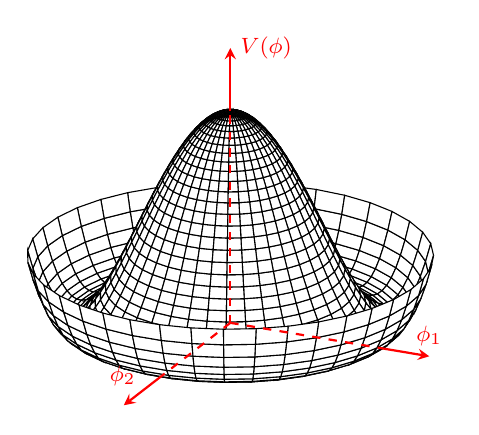
\begin{tikzpicture}

    \begin{axis}[
        %axis lines=center,
        %axis line style={->},
        hide axis,
        samples=40,
        domain=0:360,
        y domain=0:1.25,
        xtick=\empty,
        ytick=\empty,
        ztick=\empty
    ]
    \addplot3 [surf, shader=flat, draw=black, fill=white, z buffer=sort] ({sin(x)*y}, {cos(x)*y}, {(y^2-1)^2});

    \draw[red,thick,dashed] (axis cs:0,0,0) -- (axis cs:1,0,0)
                %node[below,font=\footnotesize]{$\phi_{1}$}
                ;
    \draw[red,thick,-stealth] (axis cs:1,0,0) -- (axis cs:1.35,0,0)
                node[above,font=\footnotesize]{$\phi_{1}$};

    \draw[red,thick,dashed] (axis cs:0,0,0) -- (axis cs:0,-1,0)
                node[left=2mm,font=\footnotesize]{$\phi_{2}$};
    \draw[red,thick,-stealth] (axis cs:0,-1,0) -- (axis cs:0,-1.55,0)
                %node[right=1mm,font=\footnotesize]{$\phi_{2}$}
                ;

    \draw[red,thick,dashed] (axis cs:0,0,0) -- (axis cs:0,0,1)
                %node[left=2mm,font=\footnotesize]{$\phi_{2}$}
                ;
    \draw[red,thick,-stealth] (axis cs:0,0,1) -- (axis cs:0,0,1.3)
                node[right,font=\footnotesize]{$V(\phi)$};

    \end{axis}

\end{tikzpicture}
  \caption{
    The Higgs potential $V(\phi)$ of the complex scalar field singlet $\phi = \phi_1 + i \phi_2$, with a choice of $\mu^2 < 0$ leading to a continuous degeneracy in the true vacuum states. A false vacuum is present at the origin.
  }
  \label{fig:higgs_potential}
\end{figure}
%
In order to obtain a physical interpretation of the Lagrangian in \cref{eq:sm_higgs_lagrangian} for the case where $\mu^2 < 0$, the field $\phi$ is expanded around the vacuum state.
The vacuum expectation value (VEV) is the expected value of the field $\phi$ which minimises the potential $V(\phi)$ (equivalently the expected value of the field operator $\phi$ when the system is in a vacuum state, $|\langle{\phi}\rangle_0|^2 \equiv |\bra{0} \phi \ket{0}|^2 \equiv \vev{\phi}$).
%It is worth mentioning explicitly at this point that each base operator $\phi_i$ explicitly defines its own vev $\vev{\phi_i}$
Minimising the potential gives a VEV of
%
\begin{equation}\label{eq:higgs_vev}
  \vev{\phi} = -\mu^2 / \lambda = v^2 .
\end{equation}
%
Due to the shape of the potential in \cref{fig:higgs_potential}, there is a degeneracy in the direction that the complex doublet $\phi$ points.
As all the different vacuum states minimise the potential and therefore yield identical physics, one can arbitrarily choose the state to lie along the second component of the doublet.
Application of \cref{eq:charge_operator} shows this choice is manifestly invariant under the charge operator.
This allows the identification of the unbroken subgroup $U(1)_Q$, under which the ground state is invariant.
The generator of $U(1)_Q$ is the charge operator $Q$.


%Different vacuum states are traversed by moving in flat directions of the potential.
%Particles corresponding to fluctuations of the field along the flat directions in the potential are massless as they don't cost energy to attain.

% MORE ON PHYSICAL PARTICLE INTERP AND FIELD SUBSTITUITON
%For a field to be able to have the standard particle interpretation, it must be linear in creation and annihilation operators. Such a field has a vanishing vacuum expectation value. As such, fields with nonvanishing VEV cannot correspond to particles. The new field H has vanishing VEV
%  Now considering fluctuations (particle content) around this vacuum we obtain $\phi(\mathrm{x}) = v + f(\mathrm{x})$ as the sum of the vacuum contribution and scalar particle fluctuations. In effect, this is a field substitution, where the new field has the property $\vev{f} = 0$ (i.e $f = 0$ minimises the potential $V(\phi)$).
% This is the motivation behind the field substitution in equation (4.3), where the newly introduced
%field has a vanishing VEV by construction. Note that the original field remains massless, whereas the newly
%introduced field (corresponding to a physical particle) gains mass.


Adding the particle content back to the theory by expanding the field around the vacuum state, and making a transformation to the unitary gauge to remove unphysical Nambu-Goldstone modes (which arise in the context of global symmetries \cite{PhysRev.117.648,Goldstone1961FieldTW}), yields
% adding particle content is performing a field substitution
%transformation to the unitary gauge to regain physical interpretation
%
\begin{equation}\label{eq:unitary_higgs}
  \phi = 
  \frac{1}{\sqrt{2}}
  \begin{bmatrix}
    0 \\ v + H
  \end{bmatrix} ,
\end{equation}
%
where $H$ is a real scalar field, the \textit{true vacuum} Higgs field.
Substituting this into \cref{eq:sm_higgs_lagrangian} and identifying physical fields from the quadratic terms of linear combinations of unphysical fields, one can write the physical fields $W_\mu^\pm$, $Z_\mu$ and $A_\mu$ in terms of the original fields $A^a_\mu$ and $B_\mu$.
%The physical fields are the natural mass eigenstates that yield quadratic terms of the form $m^2 \chi^\mu\chi_\mu$.
This gives
%
\begin{equation}\label{eq:ew_physical_unphysical_fields}
  W_\mu^\pm = 
  \frac{1}{\sqrt{2}} (A^1_\mu \mp i A^2_\mu)
  \quad
  \begin{bmatrix}
    A_\mu \\ Z_\mu
  \end{bmatrix} =
  \begin{bmatrix}
      \cos\theta_W &  \sin\theta_W \\ 
    - \sin\theta_W &  \cos\theta_W
  \end{bmatrix}
  \begin{bmatrix}
    B_\mu \\ A^3_\mu 
  \end{bmatrix} .
\end{equation}
%
where $\theta_W$ is the weak mixing angle defined by 
%
\begin{equation}\label{eq:ew_coupling_weak_mixing_angle}
  \cos\theta_W = \frac{g}{\sqrt{g^2 + {g^\prime}^2}} .
\end{equation}
%
The corresponding masses of the now massive vector bosons can be read off as 
%
\begin{equation}
  m_W = \frac{1}{2} g v
  \quad
  m_Z = \frac{m_W}{\cos\theta_W} , %v^2 = \frac{m_W^2}{\cos^2\theta_W} .
\end{equation}
%
while the photon remains massless.
The Higgs mass is $m_H = v \sqrt{\lambda} = \mu$.

This is the Higgs mechanism.
It maintains the renormalisability and unitarity of the SM whilst allowing the weak vector bosons to acquire mass.
In summary, an unphysical complex scalar field $\phi$ with a nonzero VEV leads to spontaneous symmetry breaking.
Due to the non-Abelian symmetry breaking, would\nobreakdash-be massless Nambu-Goldstone modes, which arise after expansion around the true vacuum state, are cancelled out by making a local gauge transformation to the unitary gauge, and instead are absorbed by the vector bosons, allowing them to acquire mass.

This sector of the SM contains four fundamental parameters that must be determined from experiment.
These can be specified by the Lagrangian parameters $g$, $g^\prime$, $v$ and $\lambda$ or the physically measurable parameters $m_Z$, $\sin\theta_W$, $m_H$ and $e$.
In the local neighbourhood around the true vacuum, the macroscopic symmetry of the system is not realised, and therefore the physical particles do not obey the original symmetry. 
However, information about the symmetry is retained through some additional constraints on the parameters of the theory.
Prior to symmetry breaking, the potential contained two terms and two constants. After symmetry breaking there are three terms but still only two constants that relate these terms. This is the vestige of the original symmetry. %Because we have related $\mu$, $\lambda$ and $v$, when these would be three independent parameters if we had no symmetry.
%Note critically that symmetry places conditions on the two interaction terms, which are related to each other through the constants $\lambda$ and $v$. As $v$ already parameterises the mass of the field $f$, these two interaction terms are described by only one additional constant $\lambda$, when in general these terms could have their own independent coupling.

Spontaneous symmetry breaking has modified the original symmetry group of the SM $SU(2)_L \times U(1)_Y \rightarrow SU(3)_C \otimes U(1)_Q$.
Three broken generators from the symmetry group $SU(2)_L \times U(1)_Y$ have been absorbed into the definition of the physical weak vector bosons, giving them mass.
The same methodology can be used to generate the fermion masses, as shown in the next section. 



\subsection{Fermionic Yukawa Coupling}\label{sec:higgs_yukawa_coupling}

Adding the masses of the fermions by hand breaks the gauge invariance of the theory.
%
\begin{comment}
the necessity for fermion masses being generated in this way is different from that of the vector bosons, which cannot have locally invariant bilinear field terms in the Lagrangian. For the fermions, we cannot write a mass term due to the 

The reason is as follows: consider the standard \textbf{Dirac mass term} that we use to give mass to particles 
%
\begin{equation}\label{dirac mass term}
    m \overline{\psi} \psi = m (\overline{\psi}_L + \overline{\psi}_R) ({\psi}_L + {\psi}_R) = m({\overline{\psi}}_L \psi_R + \overline{\psi}_R \psi_L) ,
\end{equation}
%
where the $\overline{\psi}_L \psi_L$ and $\overline{\psi}_R \psi_R$ vanish due to the anticommutation of $\gamma^5 \gamma^0 = - \gamma^0 \gamma^5$, and the fact tat $P_L P_R = P_R P_L = 0$. Concretely, we have
%
\begin{equation}\label{same chirality spinor bilinear vanishes}
    \overline{\psi}_L \psi_L = \psi^\dagger P_L \gamma^0 P_L \psi = \overline{\psi} P_R P_L \psi = 0.
\end{equation}
%
Note that $\overline{\psi}_L = \overline{\psi_L}$. Now, \cref{dirac mass term} is note invariant under electroweak gauge transformations as the LH spinors transform under $SU(2)_L$ while RH spinors transform under $U(1)_Y$ (i.e. we could do an $SU(2)$ transformation that would affect $\psi_L$ but not $\psi_R$ which is clearly not invariant). 
\end{comment}
%
Instead, we can use a Yukawa coupling between the fermion fields and the Higgs field in order to generate mass terms after spontaneous electroweak symmetry breakdown \cite{Weinberg:1967tq}.
In this way, the fermion masses are determined by both the respective couplings to the Higgs field and the VEV of the Higgs field itself, which sets the basic mass scale of the theory.

The Higgs field $\phi$ transforms as an $SU(2)$ doublet with $Y = 1/2$, as does the left-handed fermion field $\psi_L$.
The right-handed fermion field $\psi_R$ transforms as an $SU(2)$ singlet.

\subsubsection{Charged Lepton Masses}

The renormalisable and gauge invariant coupling between a fermionic field $\psi$ and a scalar Higgs field $\phi$ can be written as 
%
\begin{equation}\label{eq:yukawa_fermion_coupling}
  \mathcal{L}_{\textnormal{Yukawa}} = 
  - g_f (\overline{\psi}_L \phi \psi_R + \overline{\psi}_R \phi^\dagger \psi_L) .
\end{equation}
%
where $\psi_L = (\nu_L, e_L)$ and $\psi_R = e_R$ for the first generation leptons.
After spontaneous symmetry breaking (see \cref{sec:sm_ewsb}), the scalar Higgs field in unitary gauge \cref{eq:unitary_higgs} consists of a VEV and the true vacuum Higgs field $H$.
Substituting this in to \cref{eq:yukawa_fermion_coupling} yields
%
\begin{equation}\label{eq:lep_mass_term}
  \mathcal{L}_{\textnormal{Yukawa}} = 
  - \frac{v g_e}{\sqrt{2}} \overline{e} e
  - \frac{g_e}{\sqrt{2}} \overline{e} H e ,
\end{equation}
%
using $\overline{e} e = (\overline{e}_L + \overline{e}_R)(e_L + e_R) = \overline{e}_L e_R + \overline{e}_R e_L$.
The VEV component of $\phi$ provides the first term in \cref{eq:lep_mass_term} which is quadratic in the electron field, and can therefore be identified as the electron mass term.
An interaction term between the electron field $e$ and the true vacuum Higgs field $H$ is also present.
Mass is generated for the other charged lepton generations in the same way.

\subsubsection{Quark Masses}

The down-type quarks acquire their mass analogous to the leptons, with $\psi_L = (u_L, d_L)$ and $\psi_R = d_R$ for the first quark generation.
Mass is generated for the up-type quarks using the conjugate field to $\phi$ which transforms under $SU(2)$ as a doublet with $Y = -1/2$.
The conjugate field $\tilde{\phi}$ is constructed as
%
\begin{equation}\label{phi c field definition}
    \tilde{\phi} = 
    i \sigma_2 \phi^\dagger = 
    \begin{bmatrix}
    0 & 1 \\ -1 & 0
    \end{bmatrix} 
    \begin{bmatrix}
    {\phi_1}^\dagger \\ {\phi_2}^\dagger
    \end{bmatrix} =
    \frac{1}{\sqrt{2}}\begin{bmatrix}
      v + H \\ 0
    \end{bmatrix}
    ,
\end{equation}
%
and transforms in the same way as $\phi$. 
This field can be used to write an additional Yukawa coupling which provides mass for the up-type quarks in a similar way as before.
%
\begin{equation}\label{eq:up_quark_mass}
  \mathcal{L}_{\textnormal{Yukawa}}^{\textnormal{up}} = 
  - g_q (\overline{\psi}_L \tilde{\phi} \psi_R + \overline{\psi}_R \tilde{\phi}^\dagger \psi_L)
\end{equation}
%
Considering the first generation of up-type quarks with $\psi_L = (u_L, d_L)$ and $\psi_R = u_R$, substitution into \cref{eq:up_quark_mass} yields 
%
\begin{equation}
  \mathcal{L}_{\textnormal{Yukawa}}^{\textnormal{up}} = 
  - \frac{v g_u}{\sqrt{2}} \overline{u} u
  - \frac{g_u}{\sqrt{2}} \overline{u} H u .
\end{equation}
%
The Yukawa terms mix quarks of different generations.
Physical particles are detected in their mass eigenstates $q$, which diagonalise the mass matrix, but interact via the weak interaction according to their weak eigenstates $\tilde{q}$, which are superpositions of the mass eigenstates.
This feature of the weak sector leads to mixing between different generations of quarks.
Quark mixing can be expressed using the Cabibbo-Kobayashi-Maskawa (CKM) matrix, which specifies the strength of flavour-changing weak currents.
The entries in the matrix are enumerated as
%For example, the object that couples to the up quark is $\tilde{d} = V_{ud} d + V_{us} s$
%
\begin{equation}
    \begin{bmatrix}
        \tilde{d} \\ \tilde{s} \\ \tilde{b} 
    \end{bmatrix}
    = \begin{bmatrix}
        V_{ud} & V_{us} & V_{ub} \\  
        V_{cd} & V_{cs} & V_{cb} \\  
        V_{td} & V_{ts} & V_{tb} 
    \end{bmatrix}
    \begin{bmatrix}
        {d} \\ {s} \\ {b} 
    \end{bmatrix} ,
\end{equation}
%
% predicted to be unitary but experimentally may not be 3 sigma
where the size of the elements $|V_{pq}|^2$ measures the probability of a transition between states $p$ and $q$.

%%
%\begin{equation}\label{quark mass term}
%    \mathcal{L}_{\phi, \text{quarks}} = - \sqrt{2} \left[ \overline{L}_N f^-_{NM} \phi R_{M-} +
%    \overline{L}_N f^+_{NM} \phi^c R_{M+} + \text{h.c.}
%    \right] ,
%\end{equation}
%%



\subsection{Higgs Sector Phenomenology}\label{sec:higgs_pheno}


As previously discussed in this chapter, the Higgs field plays a key role in the SM by giving mass to fundamental particles. 
%The Higgs itself gains mass through self interaction.
The strength of the coupling between the Higgs field and another particle is proportional to that particle's mass.
This fact dictates which production mechanisms and decay modes are dominant at the \LHC.
The cross sections for different production mechanisms at a centre of mass energy \come{13} are shown as a function of the Higgs mass $m_H$ in \cref{fig:higgs_production_xs}.
At leading order in QCD, Higgs boson production occurs mainly through four modes, shown in \cref{fig:higgs_prod}.
The dominant production mode is gluon-gluon fusion ($pp \rightarrow H$), which is predominantly mediated by a virtual top quark loop.
Vector boson fusion ($pp \rightarrow qqH$) is the second most likely production mechanism, in which a pair of \Wboson or \Zboson bosons fuse to produce a Higgs after being radiated by two quarks.
Next most common is the associated production of a Higgs boson and a vector boson ($pp \rightarrow VH$), in which a pair of quarks fuse to produce a single \Wboson or \Zboson boson which radiates a Higgs.
The final of the four leading production modes is top quark fusion, in which two gluons each radiate a quark-antiquark pair, and a quark from each pair fuses to produce a Higgs boson.

\begin{figure}[!htbp]
  \centering
  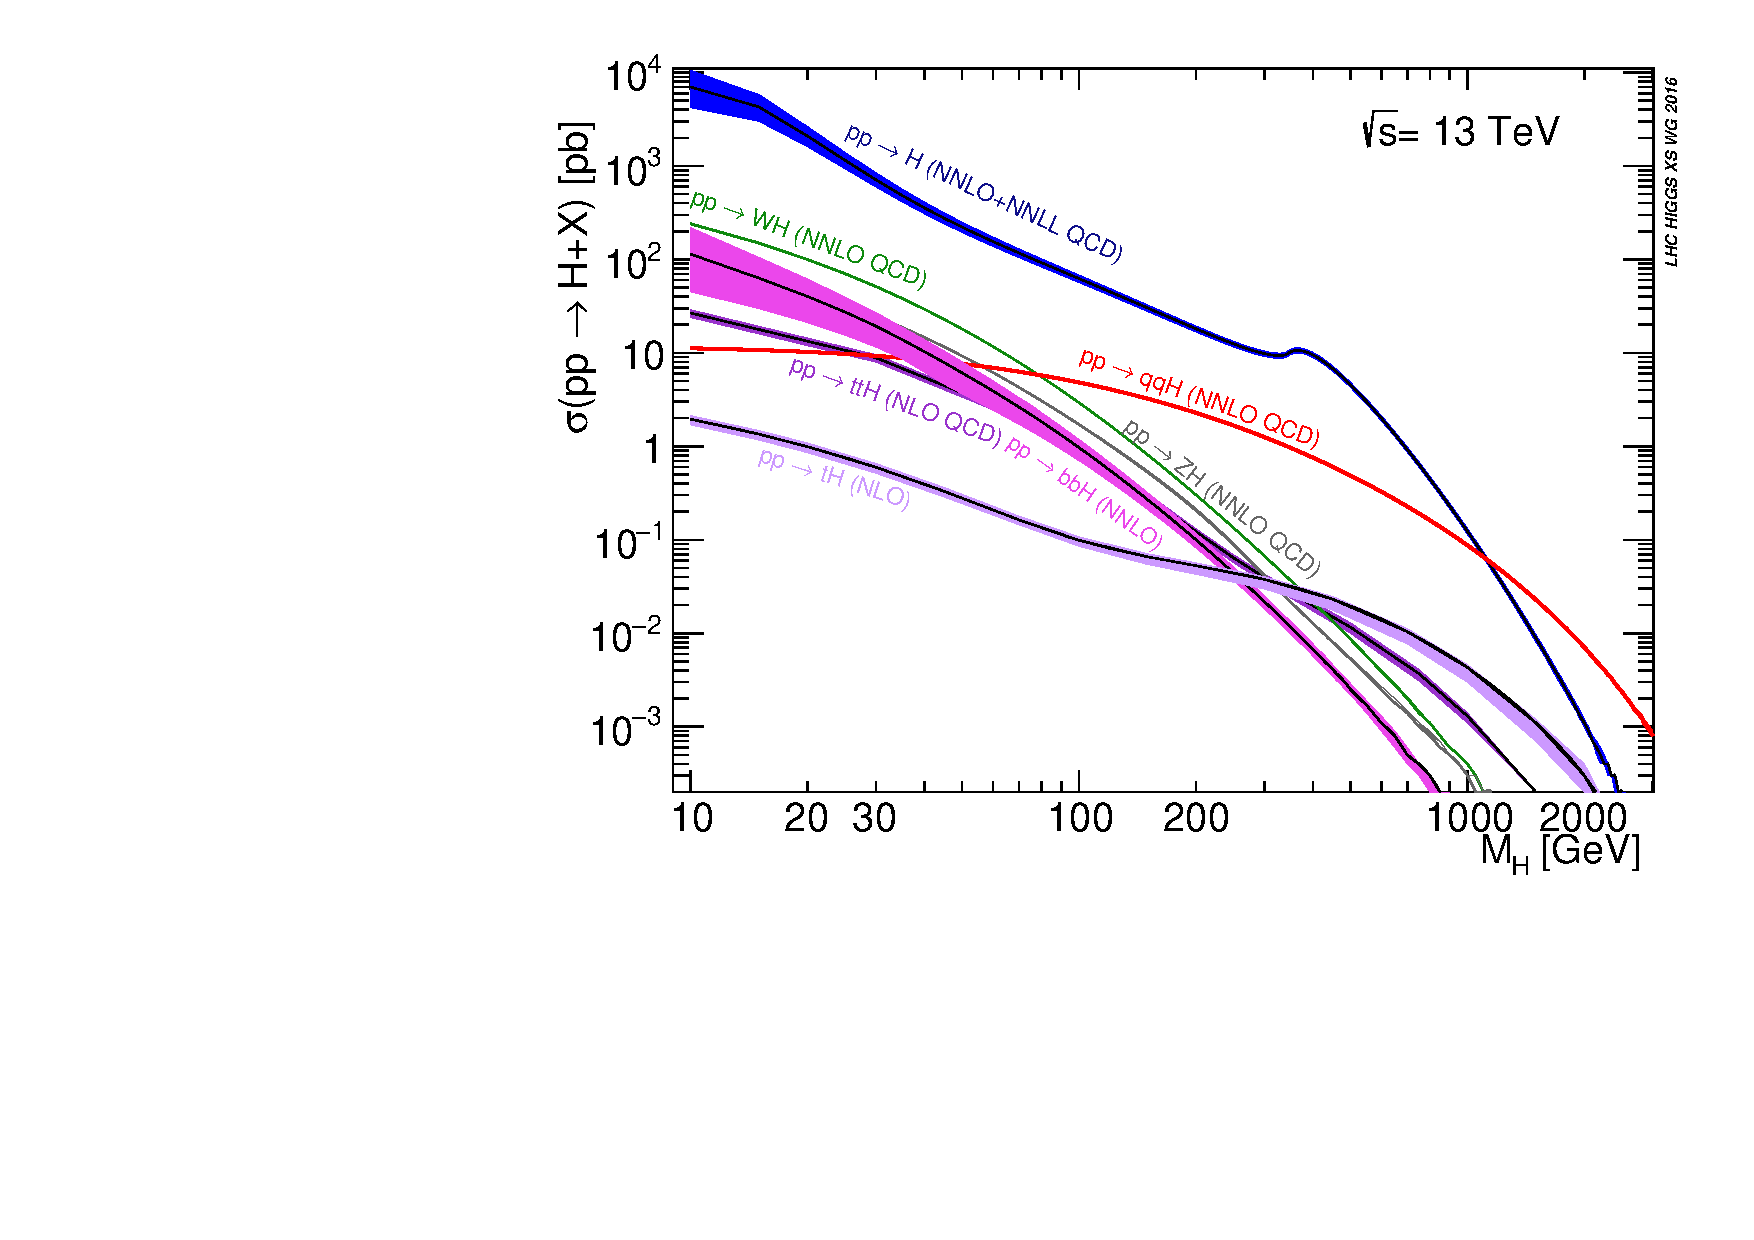
\includegraphics[width=0.65\textwidth]{chapters/1.theory/figs/plotAll_13tev_BSM_sqrt.pdf}
  \caption{
    Higgs boson production cross sections as a function of Higgs mass ($m_H$) at $\sqrt{s} = \SI{13}{\TeV}$~\cite{deFlorian:2016spz}.
    Uncertainties are shown in the shaded bands.
    At $m_H = \SI{125}{\GeV}$, Higgs boson production is dominated by gluon-gluon fusion, vector boson fusion, associated production with vector bosons, and top quark fusion.
  }
  \label{fig:higgs_production_xs}
\end{figure}

Although gluon-gluon fusion is the dominant production mode, for hadronic decays of the Higgs boson the associated production with a vector boson has the advantage of leading to a more distinct signature due to the likelihood of the vector bosons decaying leptons.
Leptons provide a clean signals to detect and trigger on.

\begin{figure}[!htbp]
  \centering
  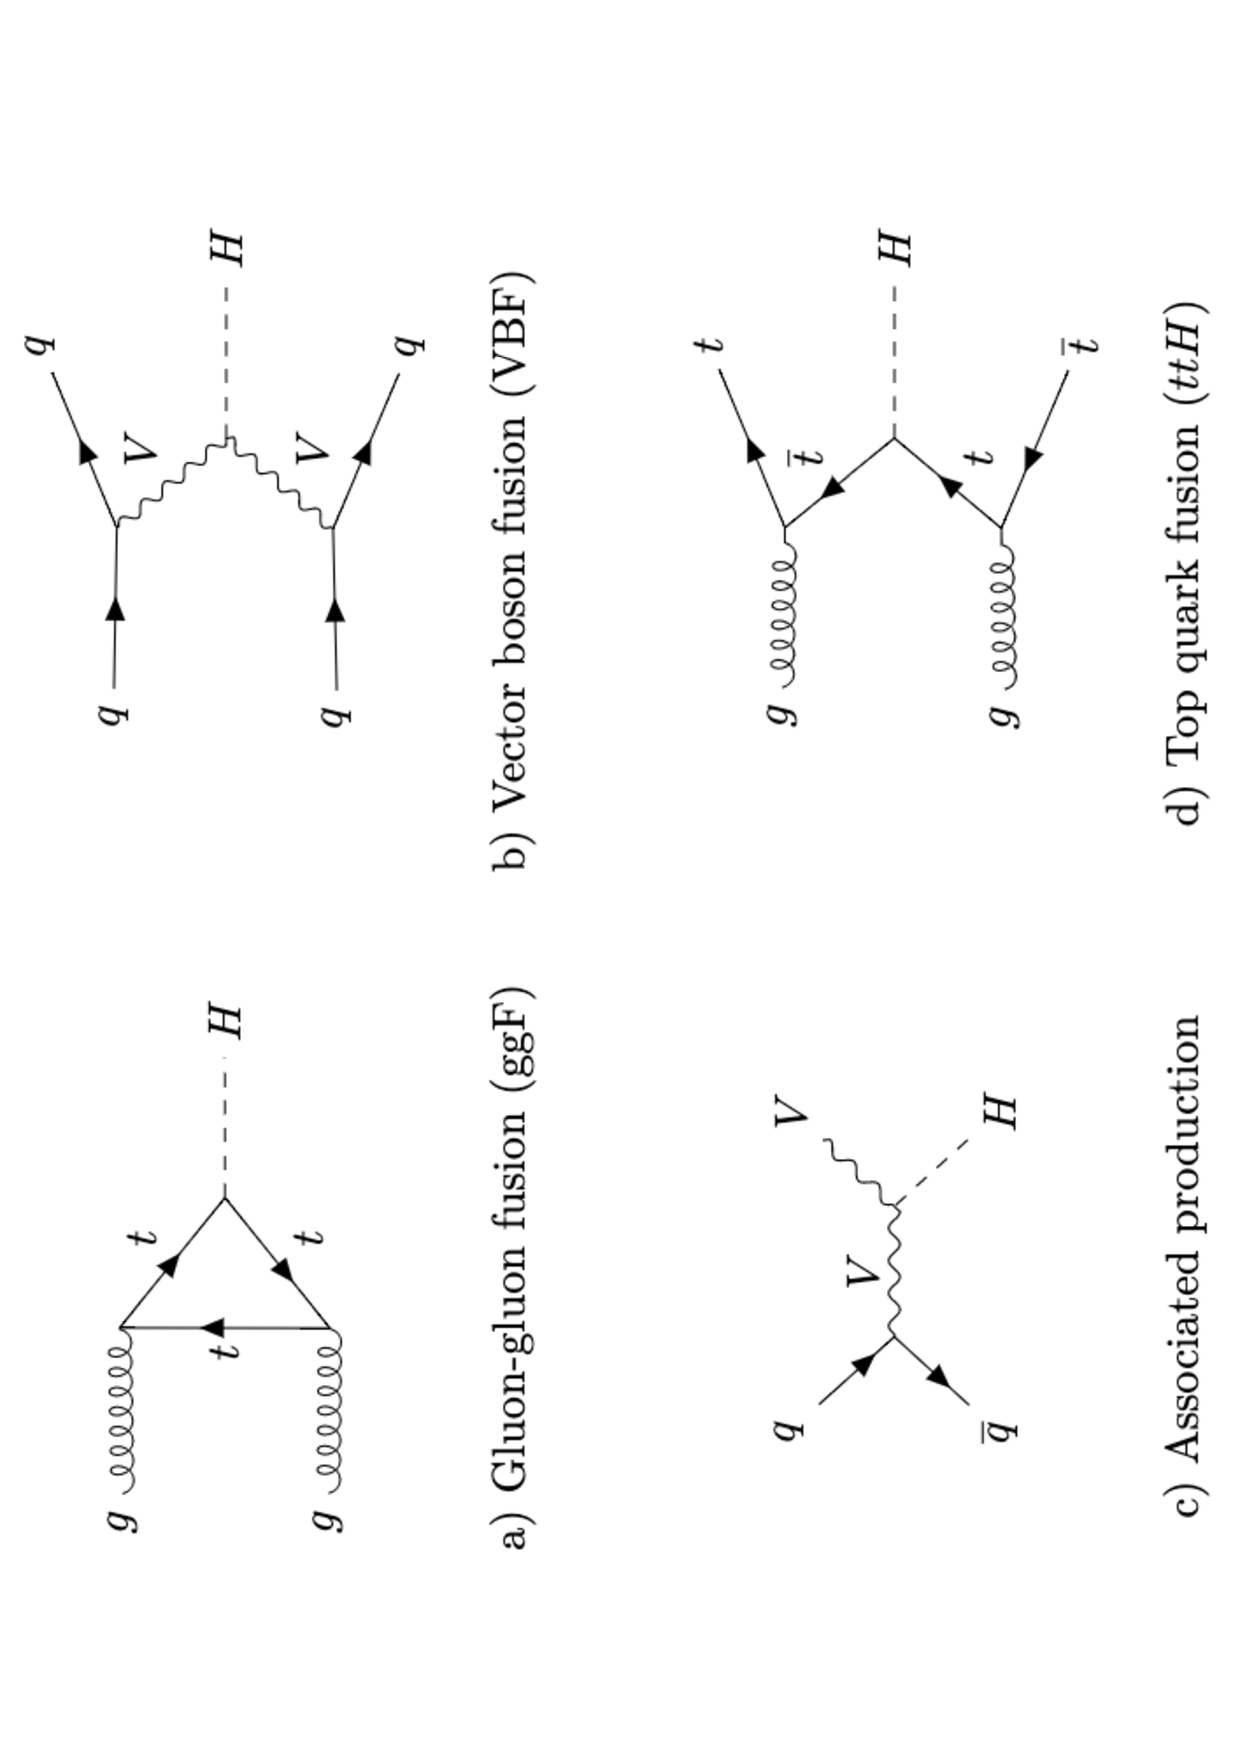
\includegraphics[angle=-90,width=0.88\textwidth]{chapters/1.theory/figs/higgs_prod.pdf}
  \caption{
    Diagrams for the four main Higgs boson production modes at the \LHC for a Higgs mass $m_H = \SI{125}{\GeV}$ at a centre of mass energy \come{13}.
  }
  \label{fig:higgs_prod}
\end{figure}

Since the Higgs boson couples proportional to mass, decays to heavier particles are favoured.
The branching ratios of different Higgs boson decay modes are shown as a function of $m_H$ in \cref{fig:higgs_br}.
Approximately \pct{58} of the time the Higgs boson decays to a pair of \bquarks, the dominant decay mode.
The next most likely decay mode is to a pair of \Wboson bosons, which occurs approximately \pct{20} of the time.
% since the Higgs it not massive enough to decay to a pair for top quarks (recall from \cref{tab:sm_fermions} $m_b = \SI{4.18}{\GeV}$ and $m_t = \SI{173}{\GeV}$).
After the \bquark, the next heaviest fermions are the tau lepton and the \cquark, decays to pairs of these particles happen approximately an order of magnitude less often.
Decays to pairs of vector bosons are via a virtual off shell Higgs boson only.
%, since the combined vector boson mass is greater than the Higgs mass.
While the \Hgammagamma and $\PH \rightarrow \Zboson \Zboson$ branching ratios are small compared with fermionic decay modes (around \pct{0.2} for \Hgammagamma), these decay channels were instrumental in the initial discovery of the Higgs due to the low level of background processes which mimic the final state \cite{HIGG-2012-27,CMS-HIG-12-028}.

\begin{figure}[!htbp]
  \centering
  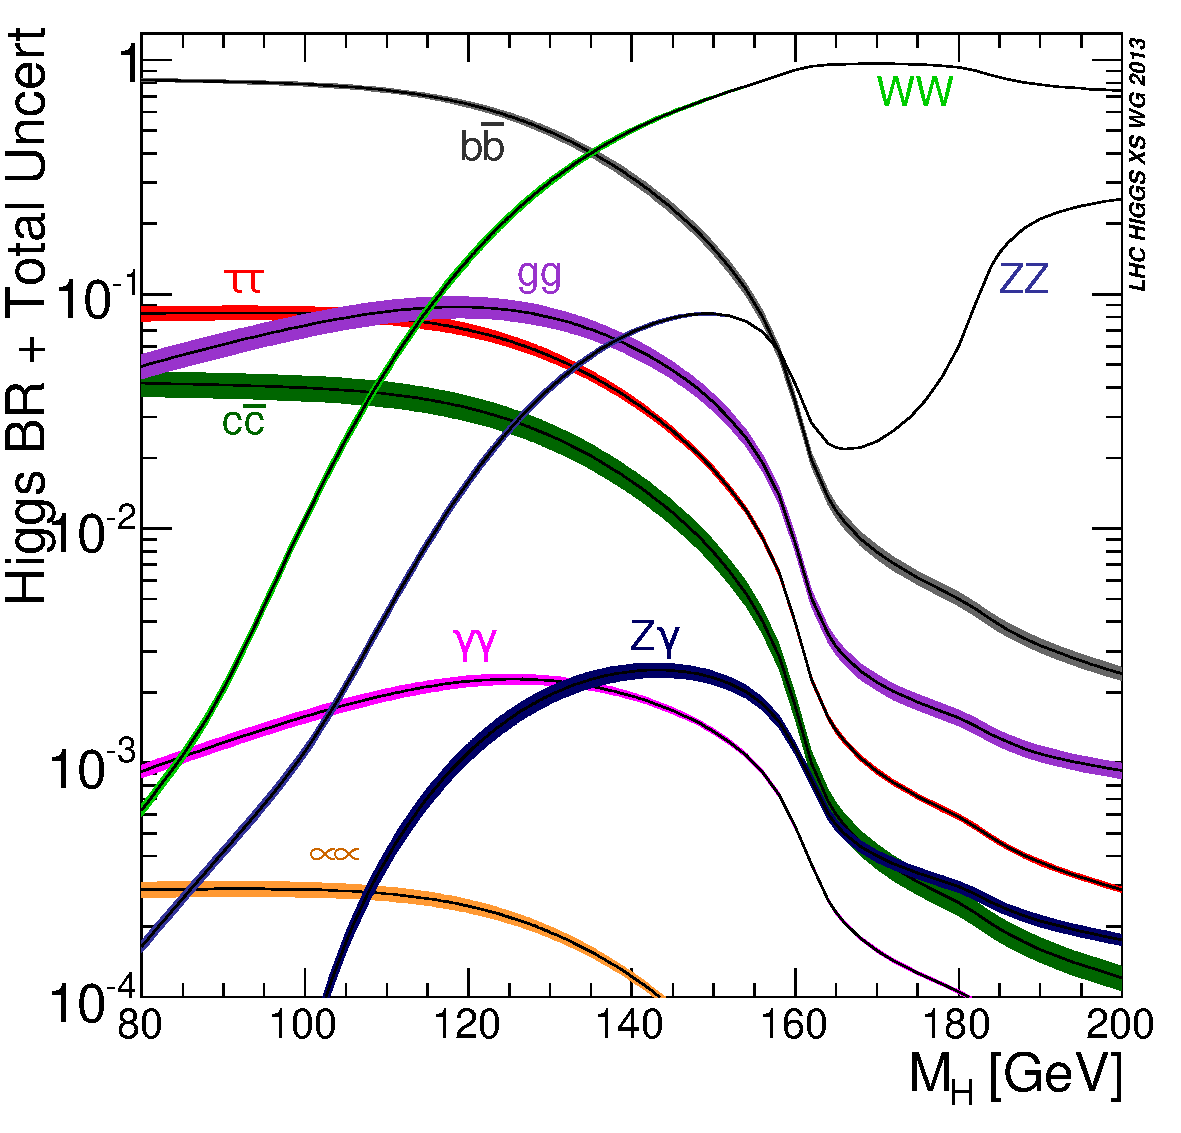
\includegraphics[width=0.5\textwidth]{chapters/1.theory/figs/Higgs_BR_LM.pdf}
  \caption{
    Higgs boson branching ratios as a function of Higgs mass ($m_H$) at $\sqrt{s} = \SI{13}{\TeV}$~\cite{deFlorian:2016spz}.
    Uncertainties are shown in the shaded bands.
    At $m_H = \SI{125}{\GeV}$, the Higgs predominantly decays to a pair of \bquarks, around \pct{58} of the time.
    The leading subdominant decay mode is to a pair of \Wboson bosons.
    }
  \label{fig:higgs_br}
\end{figure}

This thesis presents a measurement of the Higgs bosons production rate using events with a Higgs boson produced in association with vector boson and decaying to a pair of \bquarks, i.e. $pp \rightarrow VH(bb)$.
The \Hbb decay mode directly probes the Higgs coupling to fermions, and more specifically to the bottom quark.
This coupling was first observed in 2018 \cite{ATLAS-CONF-2018-036,CMS-HIG-18-016}.
Ongoing work measuring the coupling strengths, in particular in the high energy regime, is the focus of the analysis presented in this thesis in \cref{chap:vhbb_boosted}.
%\on{why interesting}
%\begin{itemize}
%  \item measure coupling to bosons and fermions (why interesting?)
%  \item Searches for non-SM Higgs decays
%  \item Searches for additional Higgs bosons
%\end{itemize}
  \chapter{The Large Hadron Collider and the \ATLAS Detector}\label{chap:lhc_atlas}

%AB: The work presented in this thesis relies on data recorded by the ATLAS detector in high energy proton-proton collisions. This chapter provides an overview of the experimental apparatus and analysis techniques used throughout this thesis.

Since the completion of its construction in 2008, the Large Hadron Collider (\LHC)~\cite{Evans:2008zzb} at \CERN has extended the frontiers of particle physics through significant increases in centre of mass energy and luminosity compared with previous collider experiments.
The \LHC accelerates bunches of protons around a \SI{27}{\km} ring until they are travelling just \SI{3}{\m\per\s} slower than the speed of light, at which point they are made to collide.
The proton bunches travel round the ring 11,000 times per second in two concentric beams, which are guided by superconducting magnets cooled using liquid helium to \SI{-271.3}{\degreeCelsius} (\SI{1.9}{\kelvin}).
The beams travel in opposite directions around the ring and are crossed at four locations so that collisisons between protons can take place.
Around these collision points four specialised detectors, ALICE~\cite{AliceCollaboration_2008}, CMS~\cite{CMS-TDR-08-001}, LHCb~\cite{LHCbCollaboration_2008} and \ATLAS~\cite{PERF-2007-01}, are located to capture information about the products of the collisions.

In this chapter, a brief overview of the \LHC and the accelerator complex at \CERN is given in \cref{sec:lhc}.
The coordinate system used at the \ATLAS detector and other common definitions are introduced in \cref{sec:atlas_coords}.
An overview of the different detector systems is provided in \cref{sec:atlas_detector}, and finally descriptions of various commonly used reconstructed objects is given in \cref{sec:physics-objects}.


\section{The Large Hadron Collider}\label{sec:lhc}

The \LHC is operated in multi-year \textit{runs} during which beams of protons are circulated and collided.
Between runs there are periods of shutdown while the accelerator and detector machinery is maintained and upgraded.
\runone began in 2010 when the \LHC collided proton bunches, each containing more than $10^{11}$ particles, 20 million times per second, providing \SI{7}{\TeV} proton-proton collisions at instantaneous luminosities of up to \peakLumi.
The centre-of-mass energy was increased to \SI{8}{\TeV} in 2012.
Over the course of \runone, \intlumirunone of usable integrated luminosity was recorded.
\runtwo, which spanned 2015--2018, further increased the proton-proton collision energy to \SI{13}{\TeV}.
During \runtwo the bunch spacing was reduced, leading to a collisison rate of \SI{40}{\mega\hertz}.
Over the course of \runtwo a total usable integrated luminosity of \intlumi was recorded. % less good for physics
2022 marked the beginning of \runthree which, with a higher center of mass energy and peak luminosity, is expected to culminate in an approximate tripling of the dataset size.
%We will be focusing the proton beams at the interaction points to less than 10 micron beam size, to increase the collision rate. (nominal beam size (width) is 16 microns from around run1)
A summary of key information about each run is listed in \cref{tab:lhc_runs}.

\begin{table}[!htbp]
  \footnotesize\centering
  \setlength{\tabcolsep}{0.5em} % for the horizontal padding
  \begin{tabular}{cc|cccc}
      \toprule\hline
      \textbf{Period} & \textbf{Year} & $\sqrt{s}$ [\unit\TeV] 
      & \angles{\mu} & \textbf{Bunch spacing} [\unit\ns] & \textbf{Luminosity} [\unit\invcmsqpersec] \\
      \hline
      Run 1 & 2010--2012 & \SIrange[range-phrase=--,range-units=single,range-exponents=combine]{7}{8}{} & 18 & 50--150 & $8 \times 10^{33}$ \\
      Run 2 & 2015--2018 & \SI{13  }{} & 34 & 25 & $1\textnormal{--}2 \times 10^{34}$ \\
      Run 3 & 2022--2025 & \SI{13.6}{} & 50 & 25 & $2 \times 10^{34}$ \\
      \hline\bottomrule
  \end{tabular}
  \caption{
    Overview of the different LHC runs \cite{atlas-lumi-run1,atlas-lumi-run2}.
    The average number of interactions per bunch-crossing is denoted as \angles{\mu} (see \cref{sec:collider_defs}), and is here averaged over the entire run.
    The luminosity is the peak instantaneous luminosity. 
    Numbers for Run 3 are preliminary and are only provided to give an indication of expected performance.
    % run 1 run 2 trigger https://cds.cern.ch/record/2058218/
    %  2-3 × 1034 cm−2 s−1 and an average pile-up of ~80 collisions/bunch-crossing
    % https://cds.cern.ch/record/2732959/files/LHCP2020_094.pdf
  }
  \label{tab:lhc_runs}
\end{table}

An overview of the accelerator complex at CERN is shown in \cref{fig:accelerator_complex}.
The LHC is at the final stage of a chain of accelerators which incrementally step-up the energy of incoming protons.
The first accelerator is Linac2 (which has been replaced by Linac4 in 2020), a linear accelerator which accelerates negative hydrogen ions to an energy of \SI{160}{\MeV}.
Upon leaving Linac4, the ions are stripped of both electrons and the resulting protons are fed into the Proton Synchrotron Booster (PSB), which increases the energy of the protons to \SI{2}{\GeV}.
The protons leaving the PSB are passed to the Proton Synchrotron (PS), which increases the energy to \SI{26}{\GeV}, and then from the PS to the Super Proton Synchrotron (SPS) which further increases the energy to \SI{450}{\GeV}.
Finally, the proton beams are injected in the LHC where they are accelerated to their final energy of \SI{6.5}{\TeV} (for \runtwo).

\begin{figure}[!htbp]
  \centering
  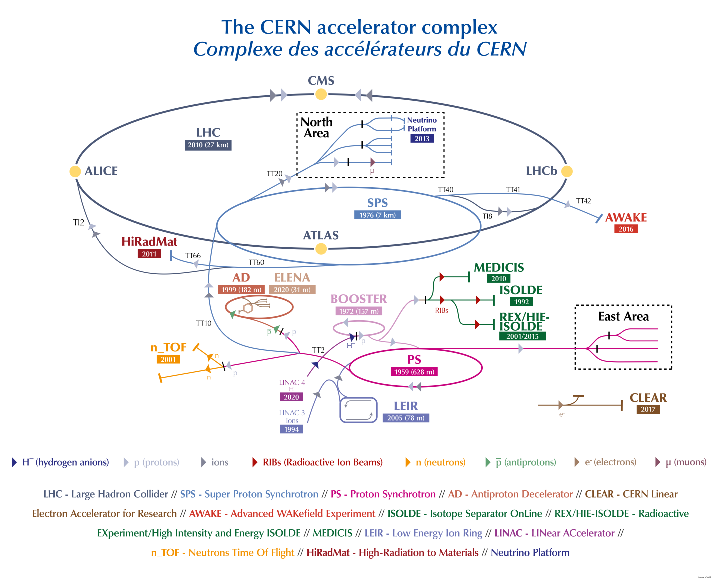
\includegraphics[width=\textwidth]{chapters/2.detector/figs/accelerator_complex.pdf}
  \caption{
    An overview of the \CERN accelerator complex \cite{CERN:2012:accelerators}.
    The \LHC is fed by a series of accelerators starting with Linac2 (or Linac4 from 2020).
    Next are the Proton Synchrotron Booster, the Proton Synchrotron, and finally the Super Proton Synchrotron which injects protons into the \LHC.
  }
  \label{fig:accelerator_complex}
\end{figure}


\section{Coordinate System \& Collider Definitions}\label{sec:atlas_coords}

In \cref{sec:coord_sys}, the coordinate system used at \ATLAS is introduced.
The parameterisation used for specifying the trajectory of charged particle tracks is described in \cref{sec:track_parameterisation}, and definitions for some frequently occurring concepts and quantities is provided in \cref{sec:collider_defs}.

\subsection{ATLAS Coordinate System}\label{sec:coord_sys}

%% based on https://twiki.cern.ch/twiki/bin/view/AtlasProtected/PubComCommonText

The origin of the coordinate system used by \ATLAS is the nominal interaction point in the centre of the detector.
As shown in \cref{fig:atlas_coord_system}, the \axis{z} points along the direction of the beam pipe, while the \axis{x} points from the interaction point to the centre of the LHC ring, and the \axis{y} points upwards.
The transverse plane lies in $x$\nobreakdash-$y$ while the longitudinal plane lies along the \axis{z}.
A cylindrical coordinate system with coordinates $(r,\phi)$ is used in the transverse plane, where $r$ is the radius from the origin and $\phi$ is the azimuthal angle around the \axis{z}.

\begin{figure}[!htbp]
  \centering
  % Author: Izaak Neutelings (June 2017)
% taken from https://tex.stackexchange.com/questions/159445/draw-in-cylindrical-and-spherical-coordinates
% Licensed under CC Attribution-Share Alike 4.0 International  https://creativecommons.org/licenses/by-sa/4.0/
% Original source https://wiki.physik.uzh.ch/cms/latex:example_spherical_coordinates
% Modifications by Giles Strong (March 2020):
% 1. Removal of some header code
% 2. Changing theta to eta
% 3. Addition of mountains
% 4. Changed "\draw[dashed,red] (O)  -- (Pxy);" to "\draw[->] (O)  -- (Pxy) node[right] {$p_t$};"
% Modifications by Giles Strong (April 2020):
% 1. Removal of Jura mountains
% 2. Rotated to be in terms of ATLAS coordinate system
% 3. Resized labels for the detectors

\tikzset{>=latex} % for LaTeX arrow head

\tdplotsetmaincoords{75}{50} % to reset previous setting 75 50
    \begin{tikzpicture}[scale=2.7,tdplot_main_coords,rotate around x=90]
    
    % variables
    \def\rvec{1.2}
    \def\thetavec{40}
    \def\phivec{70}
    \def\R{1.1}
    \def\w{0.3}
    
    % axes
    \coordinate (O) at (0,0,0);
    \draw[thick,->] (0,0,0) -- (1,0,0) node[below left]{$x$};
    \draw[thick,->] (0,0,0) -- (0,1,0) node[below right]{$y$};
    \draw[thick,->] (0,0,0) -- (0,0,1) node[below right]{$z$};
    \tdplotsetcoord{P}{\rvec}{\thetavec}{\phivec}
    
    % vectors
    \draw[->,red] (O) -- (P) node[above left] {$\overrightarrow{p}$};
    \draw[->] (O)  -- (Pxy) node[right] {$p_t$};
    \draw[dashed,red] (P)  -- (Pxy);
    \draw[dashed,red] (Py) -- (Pxy);
    
    % circle - LHC
    \tdplotdrawarc[thick,rotate around x=90,black!70!blue]{(\R,0,0)}{\R}{0}{360}{}{}
    
    % compass - the line between CMS and ATLAS has a ~12° declination (http://googlecompass.com)
    \begin{scope}[shift={(1.1*\R,0,1.65*\R)},rotate around y=12]
        \draw[<->,black!50] (-\w,0,0) -- (\w,0,0);
        \draw[<->,black!50] (0,0,-\w) -- (0,0,\w);
        \node[below right,black!50,scale=0.6] at (\w,0,0) {N};
    \end{scope}
    
    % nodes
    \node[right] at (\R,0,0) {LHC};
    \fill[radius=0.8pt,black!20!red]
        (O) circle node[left=4pt,below=5pt] {ATLAS};
    \draw[thick] (0.02,0,0) -- (0.5,0,0); % partially overdraw x-axis and CMS point
    \fill[radius=0.8pt,black!20!blue]
        (2*\R,0,0) circle
        node[right=4pt,below=2pt,scale=0.7] {CMS};
    \fill[radius=0.8pt,black!10!orange]
        ({-\R*sqrt(2)/2+\R},0,{-\R*sqrt(2)/2}) circle % 45 degrees from ATLAS
        node[left=2pt,below=2pt,scale=0.7] {ALICE};
    \fill[radius=0.8pt,black!60!green]
        ({-\R*sqrt(2)/2+\R},0,{\R*sqrt(2)/2}) circle % 45 degrees from ATLAS
        node[below=6pt,right=3pt,scale=0.7,anchor=north east] {LHCb};
    
    % arcs
    \tdplotdrawarc[->]{(O)}{0.2}{0}{\phivec}
        {above=2pt,right=-1pt,anchor=mid west}{$\phi$}
    \tdplotdrawarc[->,rotate around z=\phivec-90,rotate around y=-90]{(0,0,0)}{0.5}{0}{\thetavec}
        {anchor=mid east}{$\eta$}
\end{tikzpicture}
  \caption{
    The coordinate system used at the \ATLAS detector, showing the locations of the four main experiments located at various points around the LHC.
    The 3-vector momentum $\bm{p} = (p_x, p_y, p_z)$ is shown by the red arrow.
    Reproduced from \rcite{Strong:2020mge}.
  }
  \label{fig:atlas_coord_system}
\end{figure}


%The pseudorapidity is defined in terms of the polar angle $\theta$ as $\eta = -\ln \tan(\theta/2)$.

The polar angle $\theta$ is commonly specified in terms of the pseudorapidity $\eta$, defined as
%
\begin{equation}\label{eq:pseudorap}
  \eta = - \ln \left[ \tan \left( \frac{\theta}{2} \right) \right] .
\end{equation}
%
The pseudorapidity is a convenient quantity to work with as differences in $\eta$ are invariant under Lorentz boosts.
%In addition, particle production is constant as a function of $\eta$.

The transverse momentum \pt of an object is the sum in quadrature of the momenta in the transverse plane
%
\begin{equation}\label{eq:pt}
  \pt = \sqrt{ {p_x}^2 + {p_y}^2 } .
\end{equation}

Angular distance between two objects is measured in units of $\DeltaR$ and is defined as
%
\begin{equation}\label{eq:delta_r}
  \DeltaR = \sqrt{(\Delta\eta)^{2} + (\Delta\phi)^{2}} ,
\end{equation}
%
where $\Delta \eta$ and $\Delta \phi$ are the differences in pseudorapidity and azimuthal angle between the two objects.


\subsection{Track Parameterisation}\label{sec:track_parameterisation}

The trajectories of charged particle tracks are parameterised as a helix which is fully specified using five parameters: $(\dzero, \zzero, \phi, \theta, q/p)$.
The transverse and longitudinal impact pararameters (IP) \dzero and \zzero specify the closest approach of the trajectory of a particle to an given origin, where the hard scatter primary vertex (see \cref{sec:vertex_reco}) is used in this thesis.
$\phi$ and $\theta$ are the azimuthal and polar angles respectively, and $q/p$ is the measured charge on the track\footnote{Reconstructed charged particles are assumed to have a charge of $\pm 1$.} divided by the scalar 3-momentum.
\cref{fig:track_params} shows each of these parameters diagrammatically.

\begin{figure}[!htbp]
  \centering
  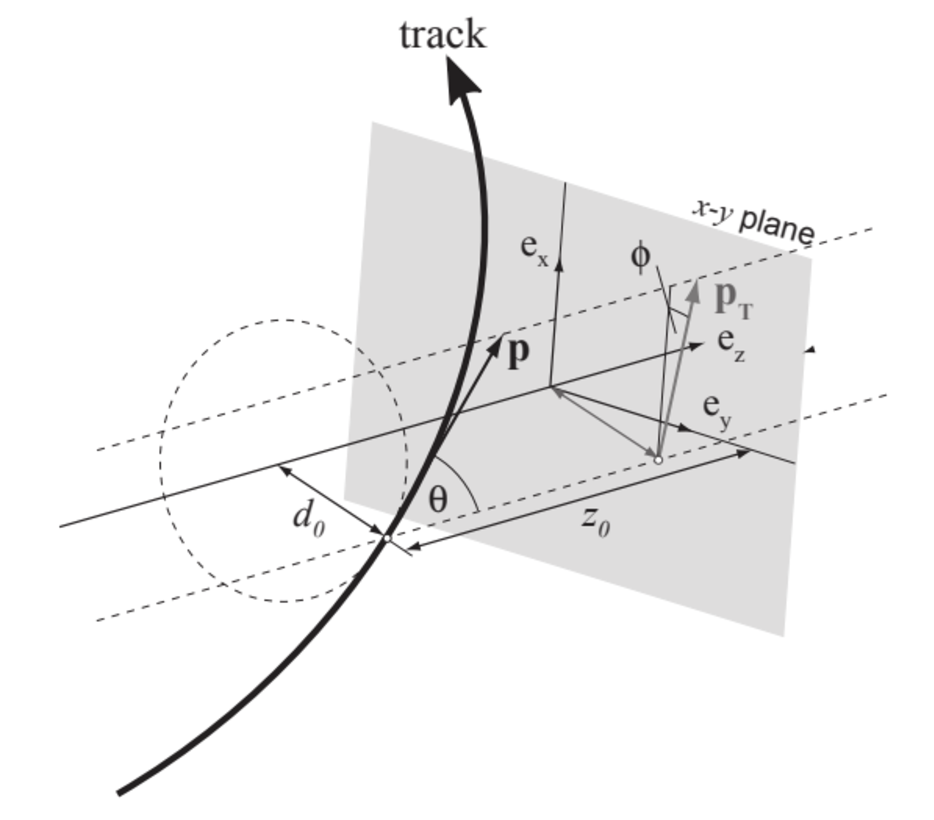
\includegraphics[width=0.75\textwidth]{chapters/2.detector/figs/track_params.pdf}
  \caption{
    The track parameterisation used at the \ATLAS detector.
    Five coordinates $(\dzero, \zzero, \phi, \theta, q/p)$ are specified, defined at the track's point of closest approach to the nominal interaction point at the origin of the coordinate system.
    The figure shows the three-momentum $\mathbf{p}$ and the transverse momentum \pt (defined in \cref{eq:pt}).
    The basis vectors $e_{\mathrm{x}}$, $e_{\mathrm{y}}$ and $e_{\mathrm{z}}$ are also shown.
    Reproduced from \rcite{atlastrackingdocs}.
  }
  \label{fig:track_params}
\end{figure}

Impact parameter significances are defined as the IP divided by its corresponding uncertainty, $\dzerosig = d_0 / \dzerouncert$ and $\zzerosig = z_0 / \zzerouncert$.
When used in flavour tagging (see \cref{chap:tracking}), track IP significances are lifetime signed according to the track's direction with respect to the jet axis and the primary vertex \cite{PERF-2012-04}.
The signed IP significances is positive if the track crosses the jet axis in front of the primary vertex and negative if the crossing is behind the primary vertex.

%\textbf{Lorentz angle}. The Lorentz angle $\theta_L$ is the angle between the electric field and the direction of the drift of the electron and holes in a silicon strip or pixel detector, when submerged in a magnetic field.

\subsection{Hadron Collider Definitions}\label{sec:collider_defs}

\subsubsection{Cross Section}
The cross section $\sigma$ is closely related to the probability of an interaction between two colliding particles, and is analogous to an effective cross-sectional area of the particles.
The cross section of a process depends on the transition matrix element and a phase space integral.
At hadron colliders such as the \LHC, the proton-proton cross section can be factorised as 
%
\begin{equation}
  \sigma(pp \to X) \approx \textnormal{PDFs} \cdot \textnormal{partonic cross section} .
\end{equation}
%
The partonic cross section can be calculated at high energies such as those found at the LHC, while the parton distribution functions (PDFs) have to be extracted from experimental results. 

\subsubsection{Luminosity}
The total number of proton-proton collisisons $N$ is related to the total $pp$ cross $\sigma$ section by the integrated luminosity $L$, as in
%
\begin{equation}
  N = \sigma L = \sigma \int \mathcal{L} ~\mathrm{d}t .
\end{equation}
%
The instantaneous luminosity $\mathcal{L}$ relates the cross section to the number of collisions per unit time.
For two colliding bunched proton beams, it is defined as
%
\begin{equation}\label{eq:lumi_def}
  \mathcal{L} = \frac{1}{\sigma} \der{N}{t} = \frac{f n_1 n_2}{4 \pi \sigma_x \sigma_y},
\end{equation}
%
where $n_1$ and $n_2$ are the number of protons in the colliding bunches, $f$ is the bunch crossing frequency, and $\sigma_x$ and $\sigma_y$ are the rms width of the beam in the horizontal and vertical directions.
%At the LHC, the beams collide with a crossing angle $\phi \approx \SI{285}{\micro\radian}$ to localise the interaction to a specific point in space.
%This reduces the effective luminosity.  

\begin{comment}  
\begin{figure}[!htbp]
  \centering
  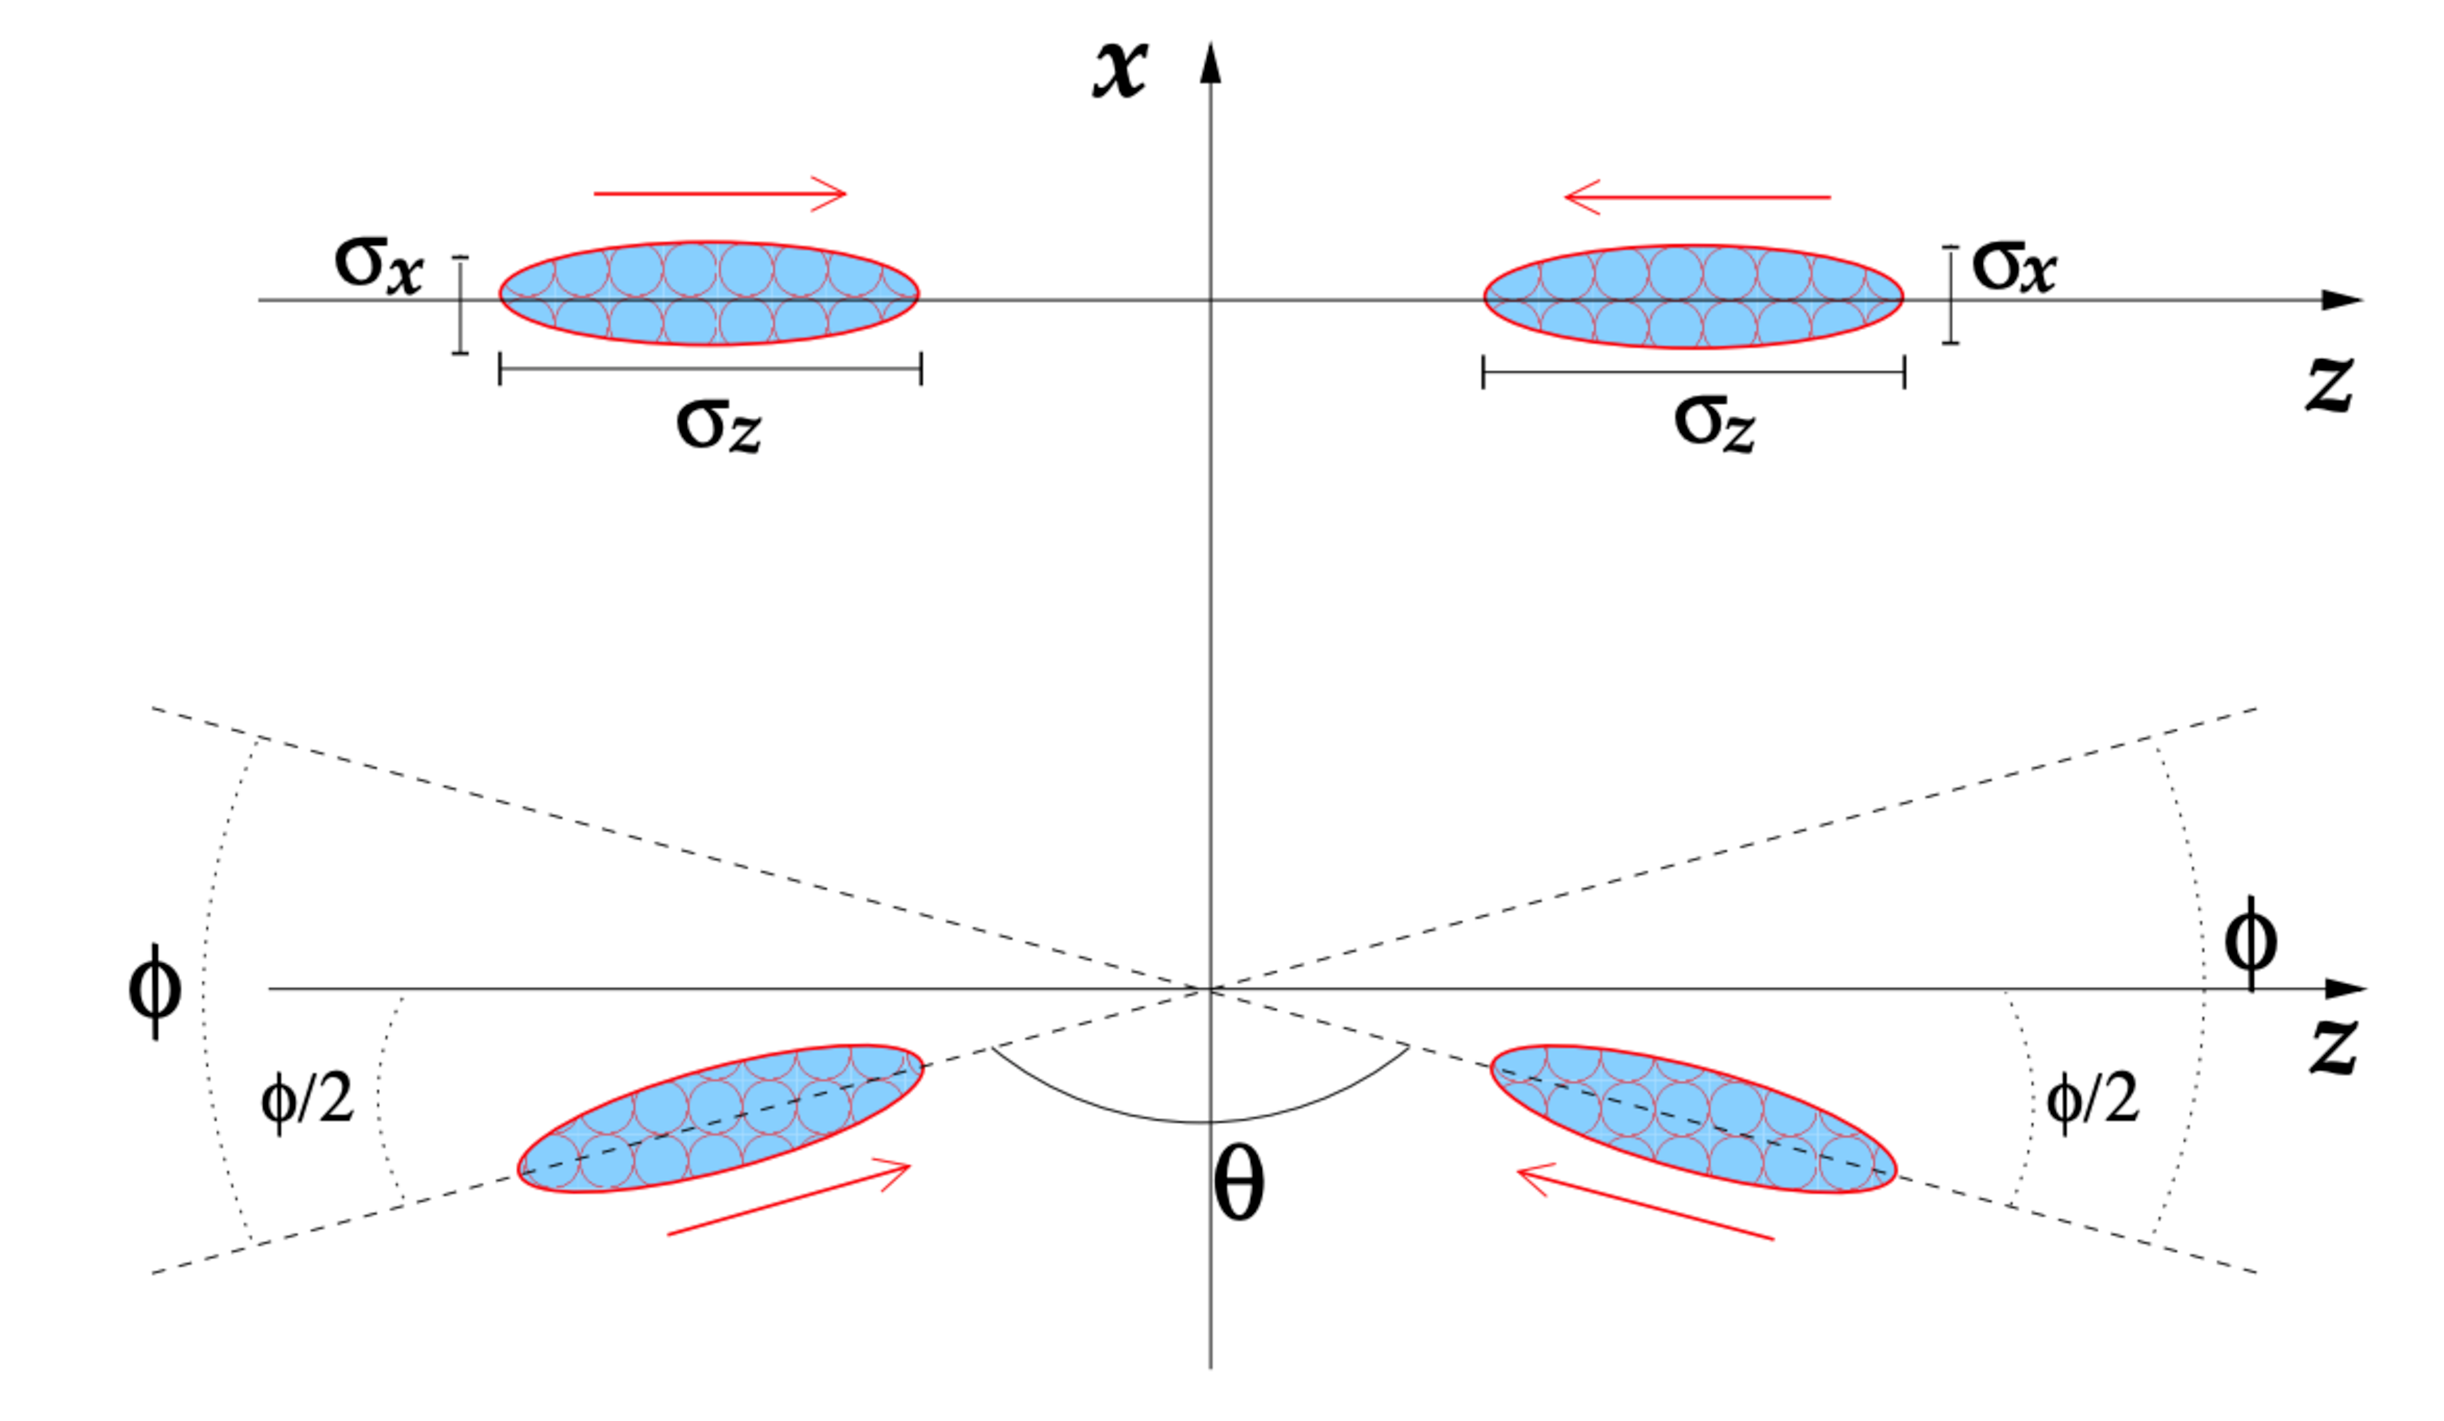
\includegraphics[width=0.6\textwidth]{chapters/2.detector/figs/beam_crossing.pdf}
  \caption{
    A digram showing the crossing of two proton bunches in the $x$\nobreakdash-$z$ plane in the case where the beams collide head on (above) and with a small crossing angle $\phi$ (below).
    %At the \LHC $\phi \approx \SI{285}{\radian}$.
    Reproduced from \cite{Cannoni:2016hro}.
  }
  \label{fig:beam_crossing}
\end{figure}
\end{comment}

The total luminosity recorded over the course of \runtwo is shown in \cref{fig:run2_lumi}. In total, \intlumi of usable physics data was collected over the three-year run.
The uncertainty on the total integrated luminosity is \pct{1.7} \cite{ATLAS-CONF-2019-021}.
%
\begin{figure}[!htbp]
  \centering
  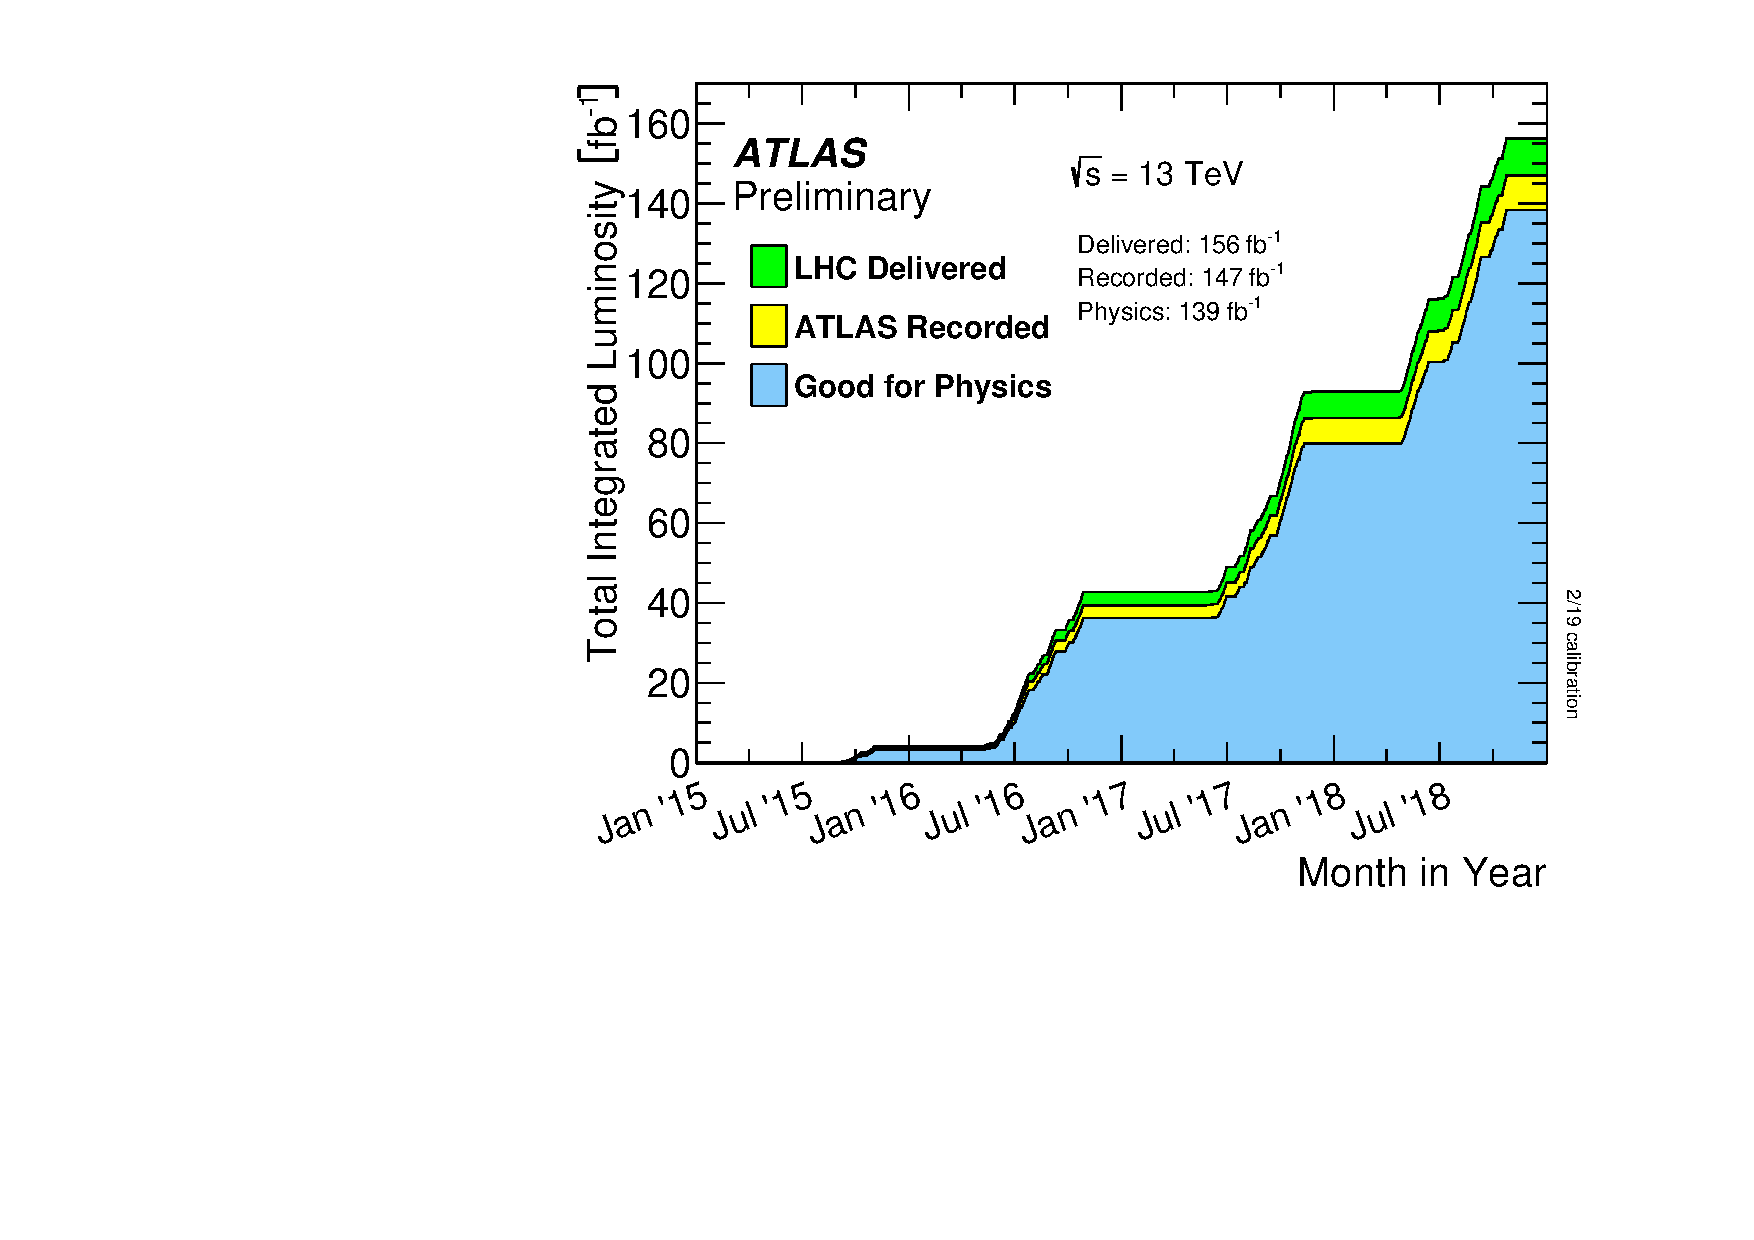
\includegraphics[width=0.6\textwidth]{chapters/2.detector/figs/intlumivstimeRun2DQall.pdf}
  \caption{
    Delivered, recorded, and usable integrated luminosity as a function of time over the course of \runtwo \cite{atlas-lumi-run2}.
    A total of \intlumi of collision data is labelled as good for physics, meaning all sub-detector systems were operating nominally.}
  \label{fig:run2_lumi}
\end{figure}
%


\subsubsection{Pile-up}

At the centre of the ATLAS detector, bunches of more than $10^{11}$ protonsare collided.
Each bunch-crossing is called an \textit{event}.
There is generally one hard proton-proton scatter per event.
Additional interactions are typically relatively soft (\lowpt) and are known as \textit{pile-up}.
%Pile-up complicates the reconstruction of the hard scatter event as results of the interactions of different proton-proton interactions have to be separated.
Pile-up from interactions within the same bunch-crossing is known as \textit{in-time} pile-up while residual signatures from previous bunch-crossings is known as \textit{out-of-time} pile-up.
The number of pile-up interactions is denoted $\mu$, which is often given as a time-averaged value \angles{\mu}.
Histograms showing the number of pile-up interactions over the course of \runtwo are shown in \cref{fig:run2_pile-up}.
%
\begin{figure}[!htbp]
  \centering
  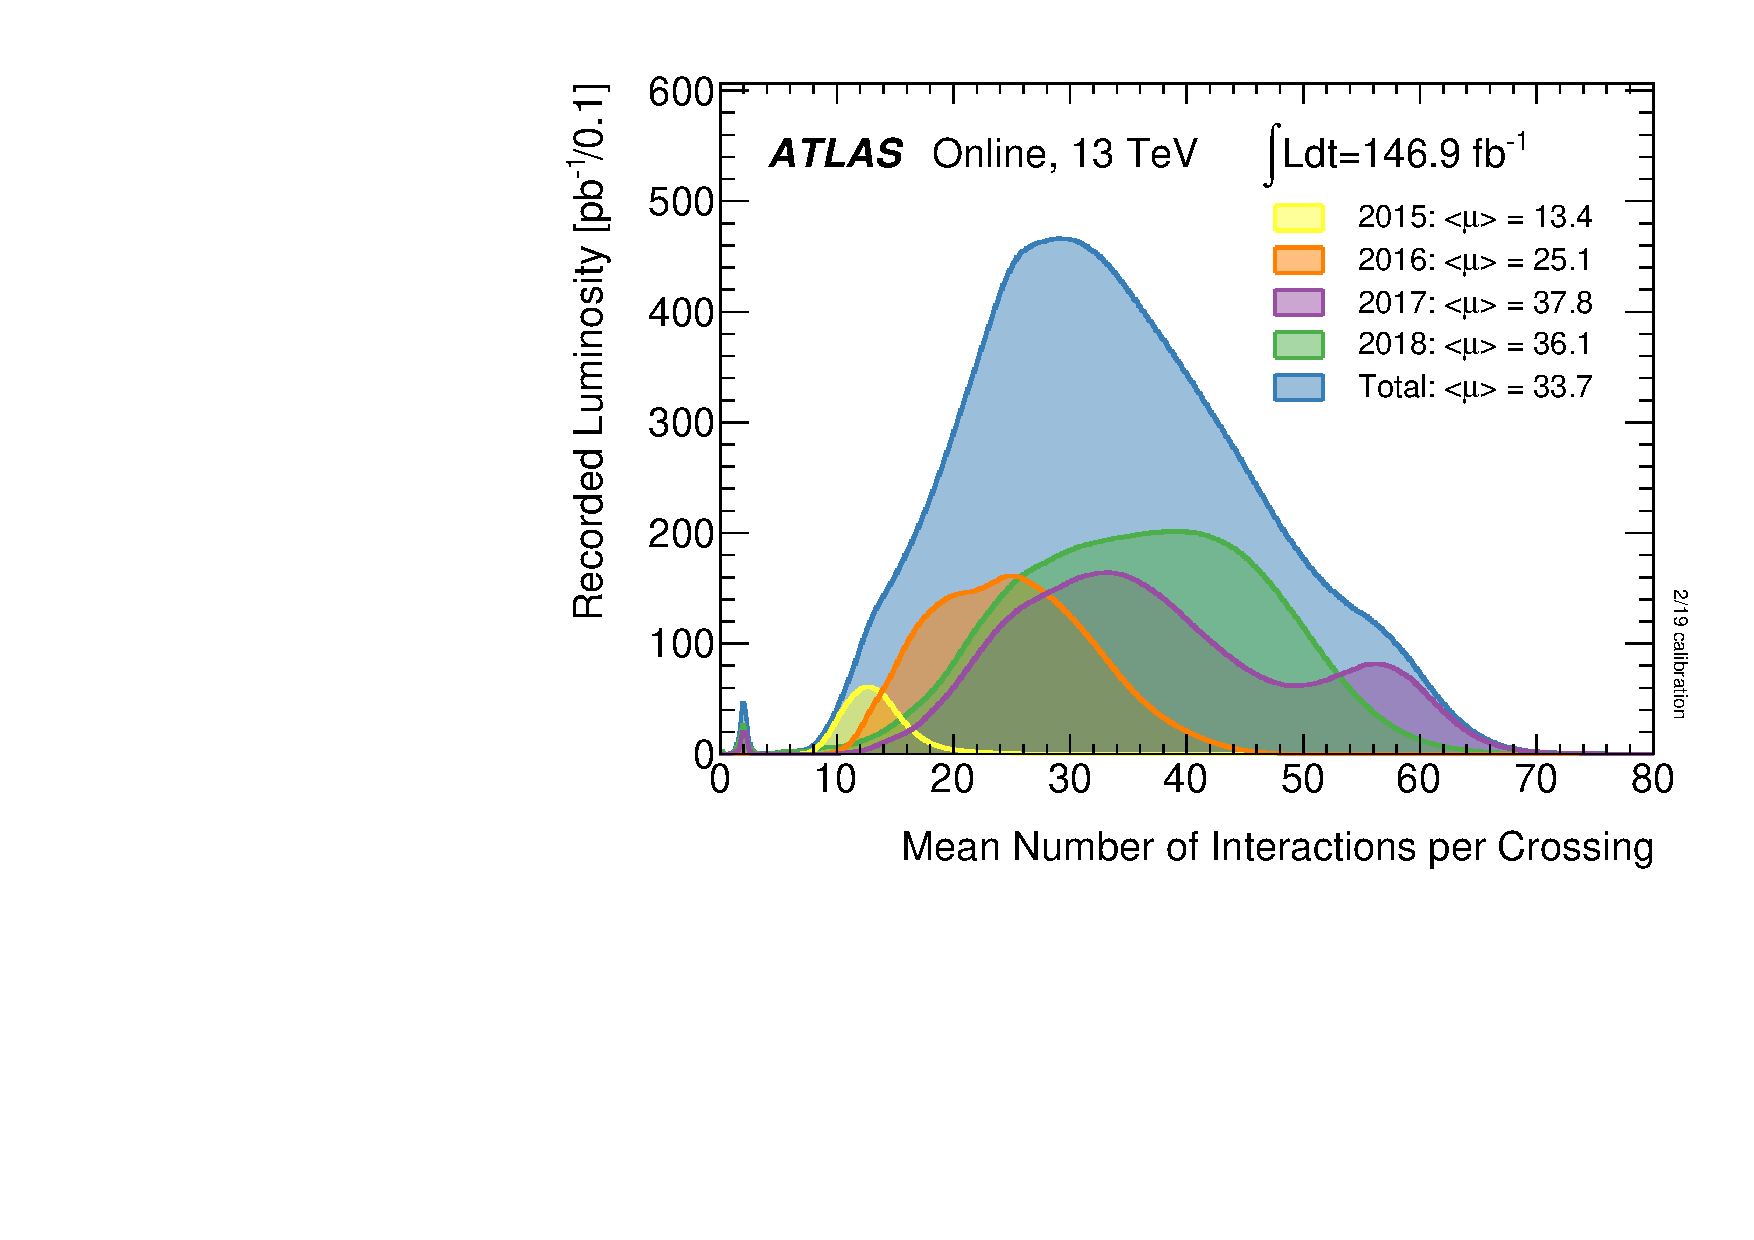
\includegraphics[width=0.6\textwidth]{chapters/2.detector/figs/mu_2015_2018.pdf}
  \caption{
    Average pile-up profiles measured by ATLAS during \runtwo \cite{atlas-lumi-run2}.
  }
  \label{fig:run2_pile-up}
\end{figure}
%


\section{The ATLAS Detector}\label{sec:atlas_detector}

The \ATLAS\footnote{\textbf{A} \textbf{T}oroidal \textbf{L}HC \textbf{A}pparatu\textbf{S}.} detector is made up of several specialised sub-detectors which are arranged concentrically around the nominal interaction point at the centre of the detector, as shown in \cref{fig:atlas_detector}.
The detector is designed to cover nearly the entire solid angle around the collision point.
In this section a brief overview of each sub-detector is given, in order of increasing radial distance from the point of collision.
The inner tracking detector is described in \cref{sec:atlas_id}, the electromagnetic and hadronic calorimeters in \cref{sec:atlas_calorimeter}, the muon spectrometer in \cref{sec:muon_spectrometer}, and finally the trigger is described in \cref{sec:trigger}.
More complete information on the detector can be found in \rcite{PERF-2007-01}, while an overview of physics performance is given in \cite{ATLAS-TDR-14}.

\begin{figure}[!htpb]
  \centering
  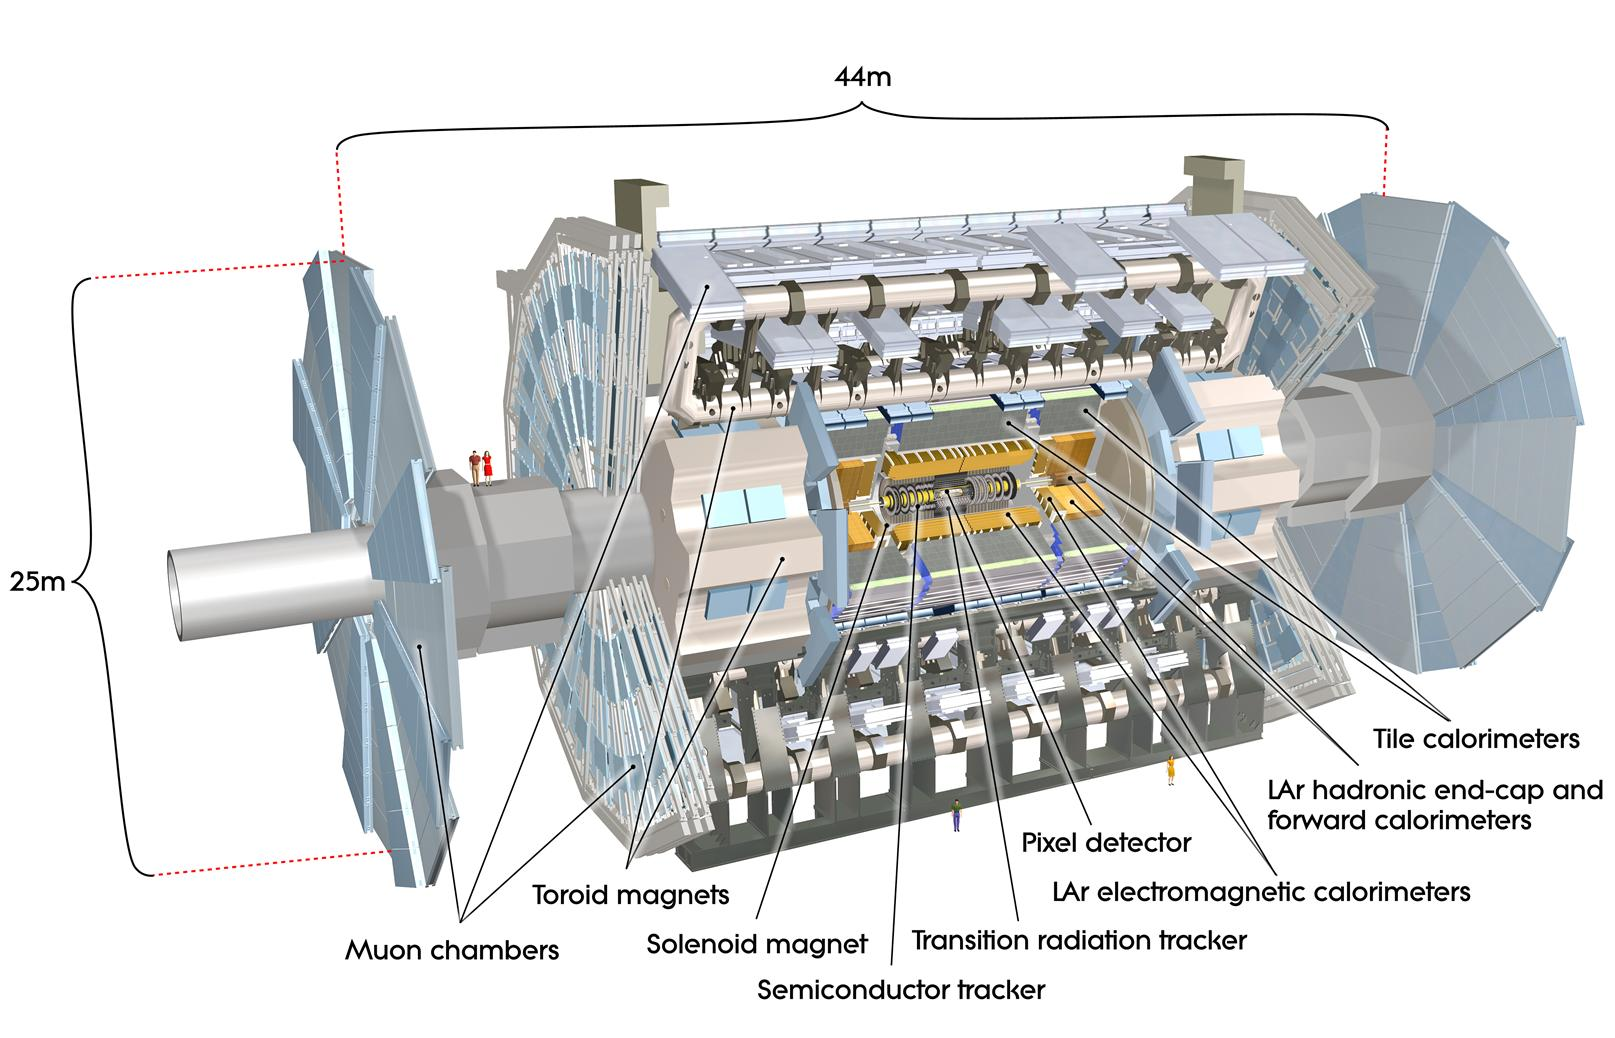
\includegraphics[width=0.9\textwidth]{chapters/2.detector/figs/atlas_detector.jpg}
  \caption{
    A 3D model of the entire \ATLAS detector \cite{Jon-And:1237407}.
    Cutouts to the centre of the detector reveal the different subdetectors which are arranged in concentric layers around the nominal interaction point.
  }
  \label{fig:atlas_detector}
\end{figure}


\subsection{Inner Detector}\label{sec:atlas_id}

The inner-detector system (ID) provides high-resolution charged particle trajectory tracking in the range $|\eta| < 2.5$.
The ID is immersed in a \SI{2}{\tesla} axial magnetic field, produced by a superconducting solenoidal magnet, which enables the measurement of particle momentum and charge.
After \runthree, the ID will be replaced by the ITk \cite{ATLAS-TDR-30,ATLAS-TDR-25}.

The inner detector is made up of several sub-systems, shown in \cref{fig:atlas_id_run1,fig:atlas_id_run2}.
The high-granularity silicon pixel detector covers the innermost region and typically provides four spacepoint measurements per track.
It is followed by the silicon microstrip tracker (SCT), which usually provides a further four spacepoint measurements (8 hits) per track.
These silicon detectors are complemented by the Transition Radiation Tracker (TRT),
which enables radially extended track reconstruction up to $|\eta| = 2.0$ and typically provides 33 (38) additional hits in the barrel (endcap). 


\begin{figure}[!htpb]
  \centering
  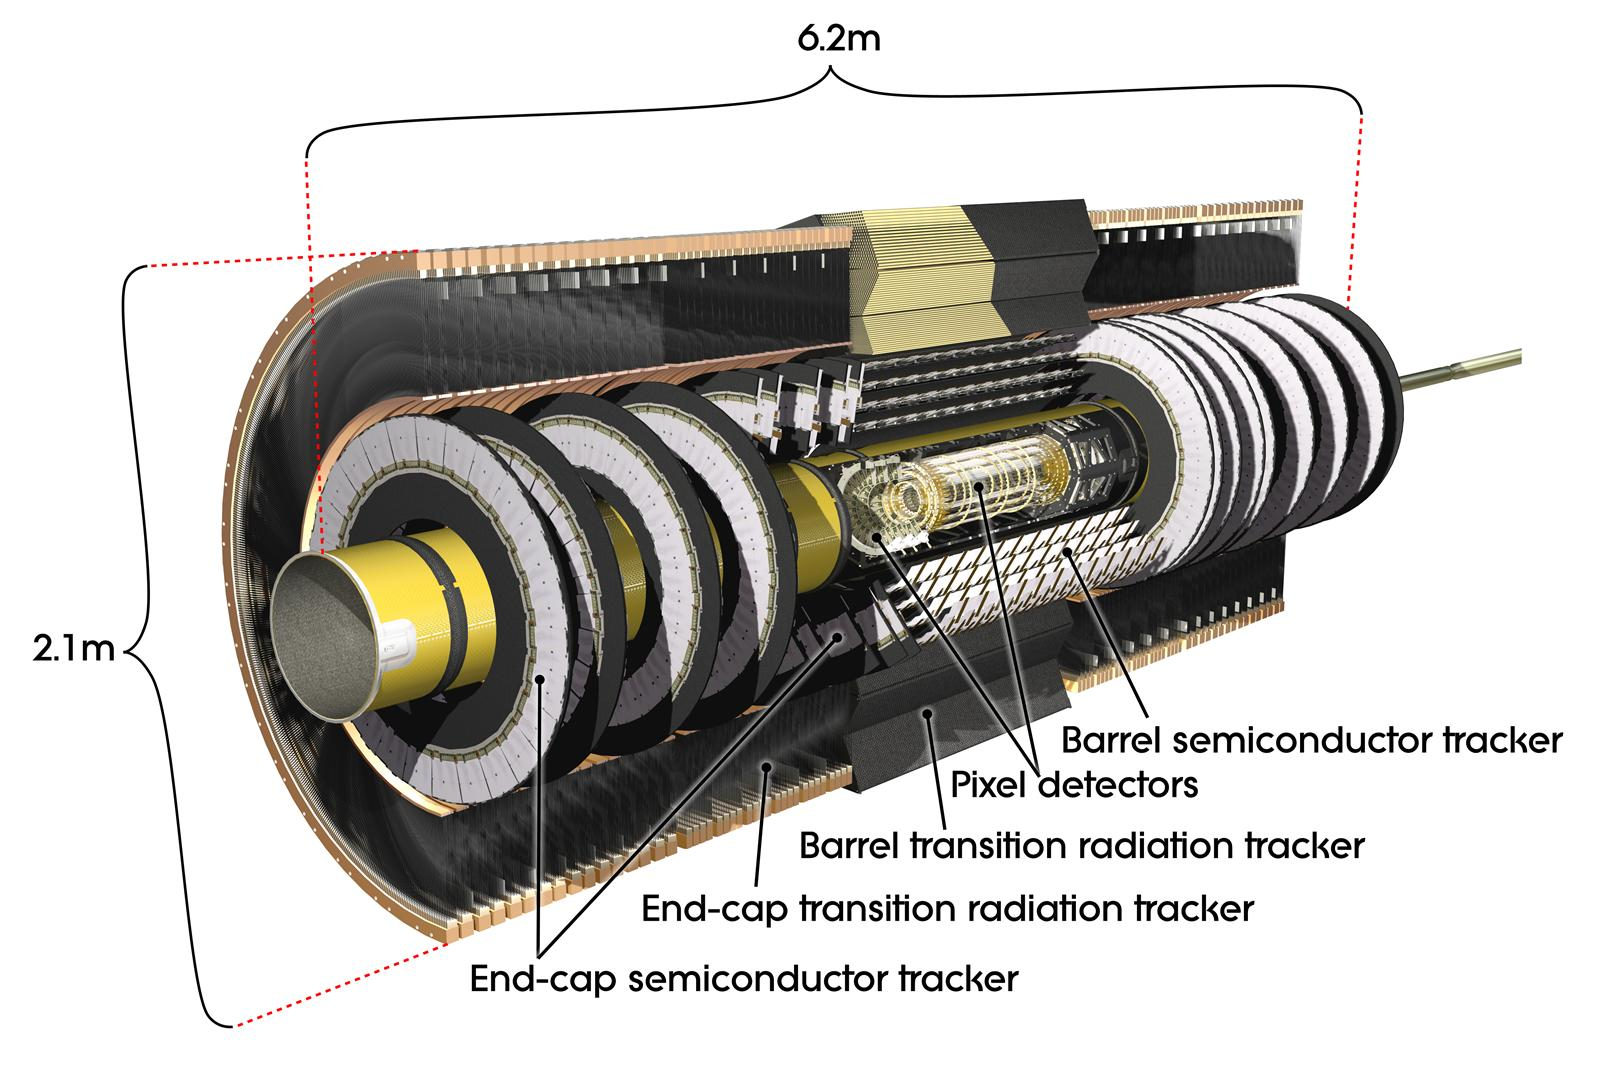
\includegraphics[width=0.75\textwidth]{chapters/2.detector/figs/atlas_id.jpg}
  \caption{
    A 3D model of the \ATLAS ID showing the pixel, SCT and TRT subdetectors \cite{atlasid}.
  }
  \label{fig:atlas_id_run1}
\end{figure}
%
\begin{figure}[!htpb]
  \centering
  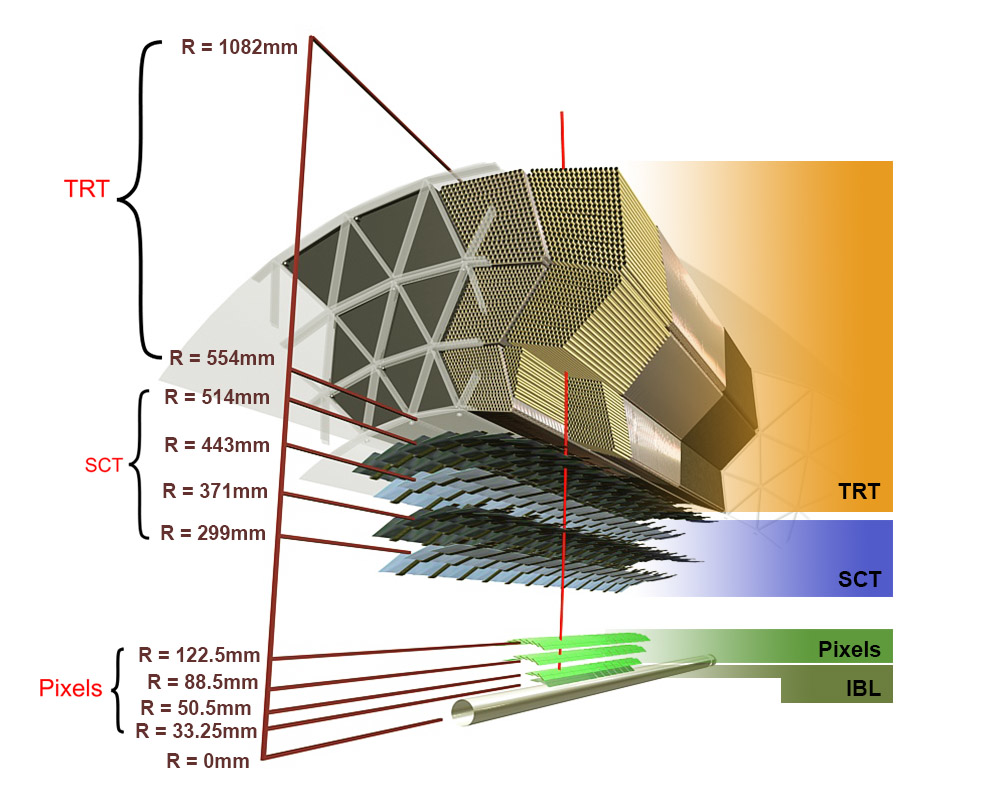
\includegraphics[width=0.75\textwidth]{chapters/2.detector/figs/atlas_id_xs.png}
  \caption{A cross-sectional view of the \ATLAS ID, with the radii of the different barrel layers shown \cite{atlastrackingdocs}.}
  \label{fig:atlas_id_run2}
\end{figure}
%

The target inverse momentum resolution for the combined ID measurement is parameterised as a function of the track transverse momentum and polar angle \cite{ATLAS-TDR-14}.
The parameterisation is given by
%
%\begin{equation}
%  \frac{\sigma_{\pt}}{\pt} = \pct{0.05} \pt \oplus \pct{1} .
%\end{equation}
\begin{equation}
  \sigma(1/\pt) = 0.36 \oplus \frac{13}{\pt \sin\theta} ~\SI{}{\per\TeV} ,
\end{equation}
%
where $\oplus$ denotes a sum in quadrature.
For \lowpt tracks (e.g. $\pt \approx \SI{500}{\MeV}$) in the central region this corresponds to a relative error of approximately \pct{0.01}.
Meanwhile for \highpt tracks (e.g. $\pt \approx \SI{100}{\GeV}$) in the central region this corresponds to a relative error of approximately \pct{4}.
The momentum resolution generally good enough to correctly identify the sign of the charge on particles up to the highest energies expected at the \LHC.
The transverse impact parameter resolution $\sigma(\dzero)$ is parameterised similarly as
%
\begin{equation}
  \sigma(\dzero) = 11 \oplus \frac{115}{\pt \sin\theta} \SI{}{\micro\meter} .
\end{equation}
%
Typical uncertainties for the transverse IP resolution are \SI{230}{\micro\meter} and \SI{11}{\micro\meter} for low and \highpt tracks in the central region, respectively.

\subsubsection{Pixel Detector}
The silicon pixel detector is comprised of four cylindrical barrels at increasing radii from the beamline, and four disks on each side.
The innermost barrel layer is the insertable B-layer (IBL), shown in \cref{fig:atlas_ibl}.
The IBL was installed before \runtwo \cite{ATLAS-TDR-19,PIX-2018-001} and lies approximately just \SI{33}{\milli\meter} from the beam axis.
The second-to-innermost layer is often referred to as the B-layer.
%Radiation-hard electronics are used to read out the 140 million channels.
The specification of the pixel detector determines the impact parameter resolution and the ability to reconstruct primary and secondary vertices.
The detector is required to have a high granularity (i.e. resolution) to maintain the low occupancy required to resolve nearby particles. %(high sparsity to resolve different tracks).
Individual pixels are \SI{50}{\micro\meter} in the transverse direction $R\phi$ and \SI{400}{\micro\meter} in the longitudinal $z$ direction (\SI{250}{\micro\meter} for the IBL).
Cluster positions have a resolution of approximately \SI{10}{\micro\meter} in $R\phi$ and \SI{100}{\micro\meter} in $z$.

%giving a resolution of 10 µm in the transverse direction and 115 µm in the longitudinal direction in the barrel region.
%For the IBL, pixels are \SI{50}{\micro\meter} in the $R\phi$ direction and \SI{250}{\micro\meter} in the $z$ direction, giving a cluster resolution of 10 µm in the transverse direction and 115 µm in the longitudinal direction in the barrel region.
%%Pixel clusters and provide an Xlocal resolution of about 10 µm, depending on the particle incident angle

\begin{figure}[!htpb]
  \centering
  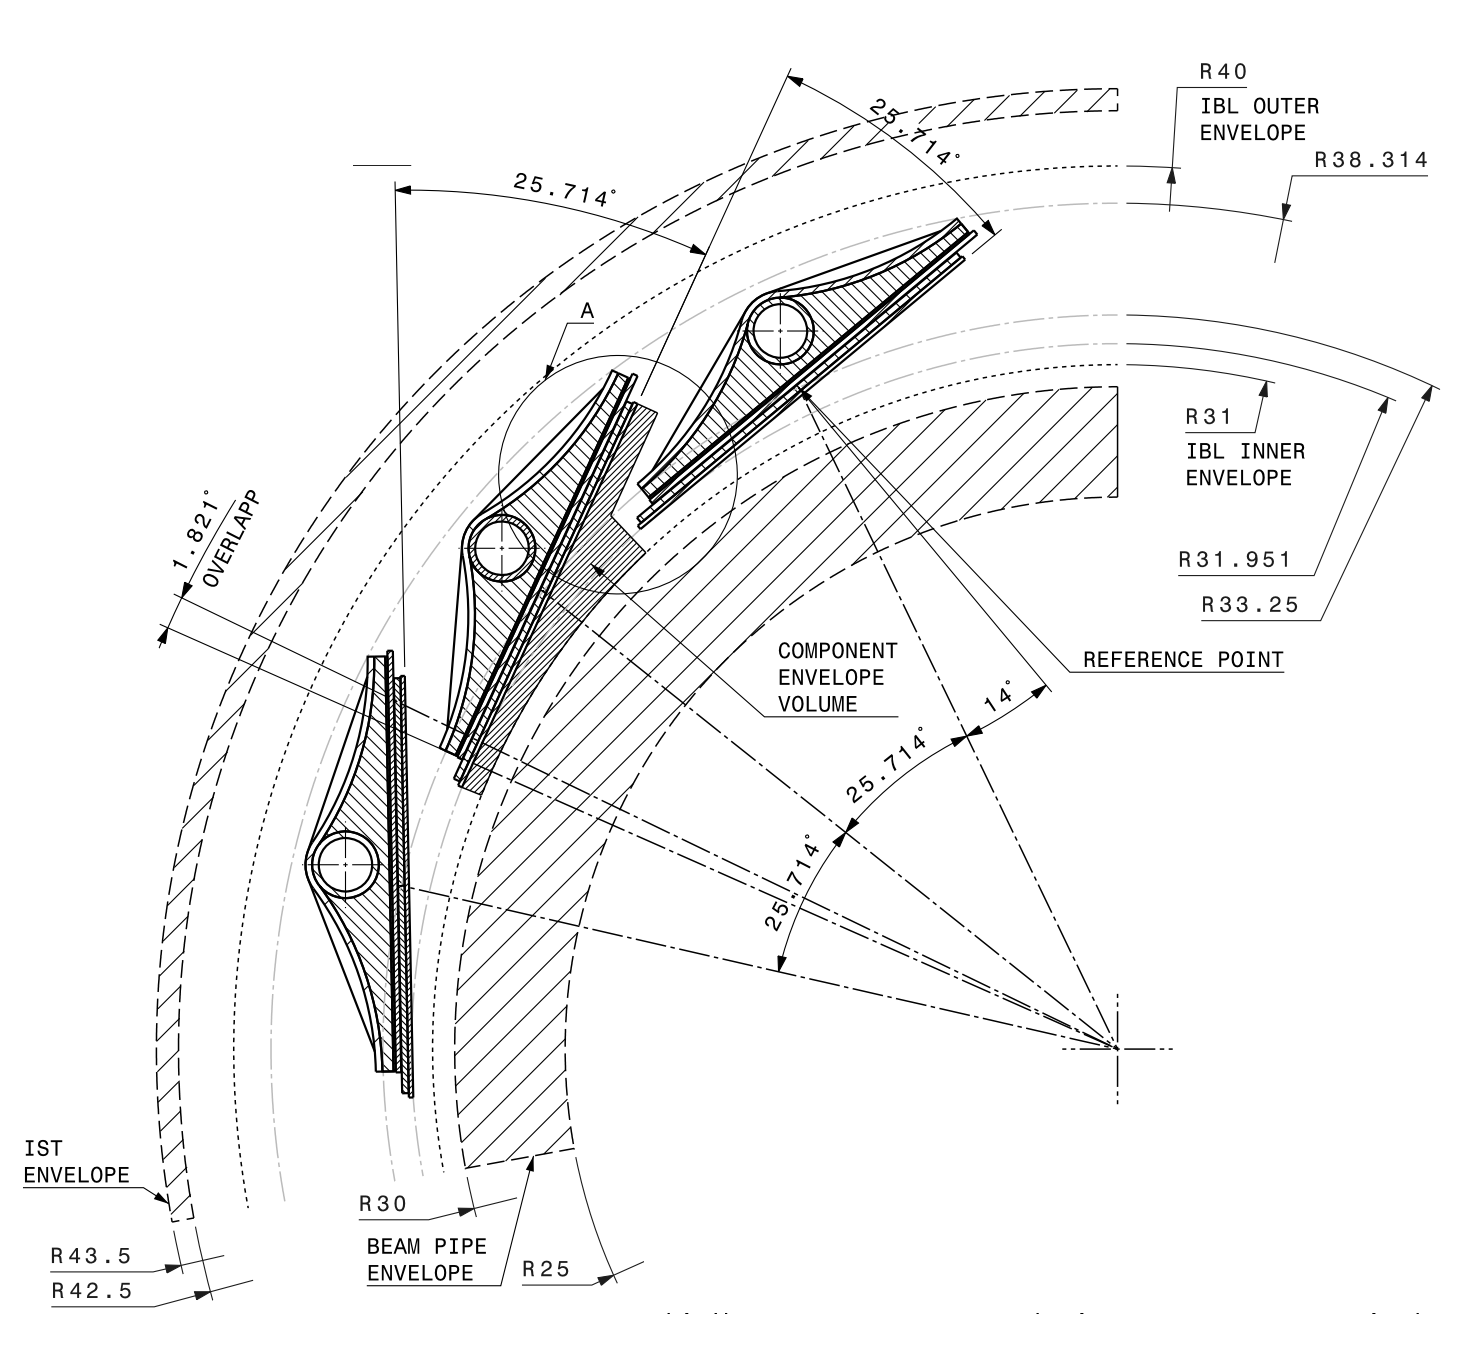
\includegraphics[width=0.6\textwidth]{chapters/2.detector/figs/atlas_ibl.png}
  \caption{A schematic cross-sectional view of the \ATLAS IBL \cite{ATLAS-TDR-19}.}
  \label{fig:atlas_ibl}
\end{figure}

\subsubsection{Semi-Conductor Tracker (SCT)}
The SCT is made up of four concentric barrel layers in the central region, and nine disks in each end-cap.
Each layer is itself made of a pair of silicon microstrip layers, with a small stereo angle (\SI{20}{\milli\radian}) between the two layers enabling the $z$\nobreakdash-coordinate to be measured from a pair of strip measurements.
The SCT typically provides four precision spacepoint measurements (eight strip measurements) per track in the barrel region.
These have intrinsic uncertainties of \SI{17}{\micro\meter} in the transverse direction $R\phi$, and \SI{580}{\micro\meter} in the longitudinal direction $z$ \cite{IDET-2013-01}.
The measurements provide a contribution to the measurement of charged particle momentum and impact parameter.
%The high granularity enables good pattern recognition
%Charge-particle tracks can be distinguished if separated by more than $\sim \SI{200}{\micro\meter}$.
%Hits are registered as binary signals if the pulse height in a channel exceeds a certain threshold.


\subsubsection{Transition Radiation Tracker (TRT)}
The TRT is a straw-tube tracker which complements the higher-resolution silicon-based tracks by offering a larger number of hits per track (typically more than 30) and a long lever arm, which aids the accurate measurement of particle momentum. 
It is made up of approximately \num{300000} drift tubes with a diameter of \SI{4}{\milli\meter} which are filled with an argon/xenon gas mixture.
The walls of each tube are electrically charged, and a thin conducting wire runs along the center.
When a charged particle traverses a tube, it ionises the gas and the resulting liberated electrons drift along the electric field to the wire, where an associated charge is registered.
In the barrel the straws run parallel to the \axis{z} and therefore the TRT only provides tracking information in $R\phi$. Straws are arranged radially in the end-caps. The resulting two-dimensional spacepoints have a resolution of approximately \SI{120}{\micro\meter}.
The spaces between the straws are filled with a polymer which encourages the emission of transition radiation, aiding electron identification.

%It allows the ID to reconstruct $V_0$s which are especially interesting in CP-violating $B$ decays.
%Electron identification capability is added by employing xenon gas to detect transition-radiation photons created in a radiator between the straws. In addition it provides additional discrimination between electrons and hadrons
% provides electron identification information based on the fraction of hits (typically 30 in total) above a higher energy-deposit threshold corresponding to transition radiation.
%may be emitted by highly relativistic charged particles as they traverse a material boundary. This effect depends on the relativistic factor γ = E/m and is strongest for electrons, 
%means it can be used for particle identification (section 6). Typical photon energies are 5–30 keV. These soft X-rays can be absorbed by Xe atoms, depositing additional energy in the gas and leading to significantly higher readout signals. Suc

%Within the radial space available, the straw spacing has been optimised for tracking at the expense of electron identification, which would be improved by a greater path length through the radiator material and fewer active straws. 


% TR is a form of electromagnetic radiation emitted when a charged particle passes through inhomogeneous media, such as a boundary between two different media. The probability that a particle emits radiation is given by it's $\gamma$ (Lorentz) factor (ie particle velocity). Electrons in general have higher Lorentz factors than eg. pions, as they are lighter than pions. In this way, the TRT discriminates between lighter and heavier particles.

\subsection{Calorimeters}\label{sec:atlas_calorimeter}

The calorimeter system measures the energy of incident particles over the range $|\eta| < 4.9$.
There are two main sub-systems: the electromagnetic calorimeter (ECal), which focuses on the measurement of electrons and photons, and the hadronic calorimeter (HCal), which measures the energy of hadrons.
A schematic view of the calorimeter system is shown in \cref{fig:atlas_calos}.
Upon entering the calorimeter, incident particles will interact with the detector material to produce a shower of secondary particles with reduced energies. 
The charge deposited in this process is measured to reconstruct the energy of the initial incident particle.
The two calorimeter sub-systems must provide strong containment of showering particles to prevent punch-through of EM and hadronic particles to the HCal and muon systems respectively.


%the fine granularity of the EM calorimeter is ideally suited for precision measurements of electrons and photons. The coarser granularity of the rest of the calorimeter is sufficient to satisfy the physics requirements for jet reconstruction and $E_T^{\textrm{miss}}$ measurements.     

%A narrow transverse profile is characteristic of an electromagnetic cascade. Hadrons passing through matter also initiate cascades through inelastic hadron-nuclei interactions. The shower produces secondary hadrons and leptons and has a comparatively wide transverse profile. 

%Nuclear interaction length is the mean distance travelled by a hadronic particle before undergoing an inelastic nuclear interaction.
%The nuclear interaction length is about an order of magnitude greater than the radiation length of the material. Therefore, like most general purpose experiments, ATLAS uses two different calorimetry systems to measure electrons and photons (the ECal) and hadrons (the HCal). 

%
\begin{figure}[!htpb]
  \centering
  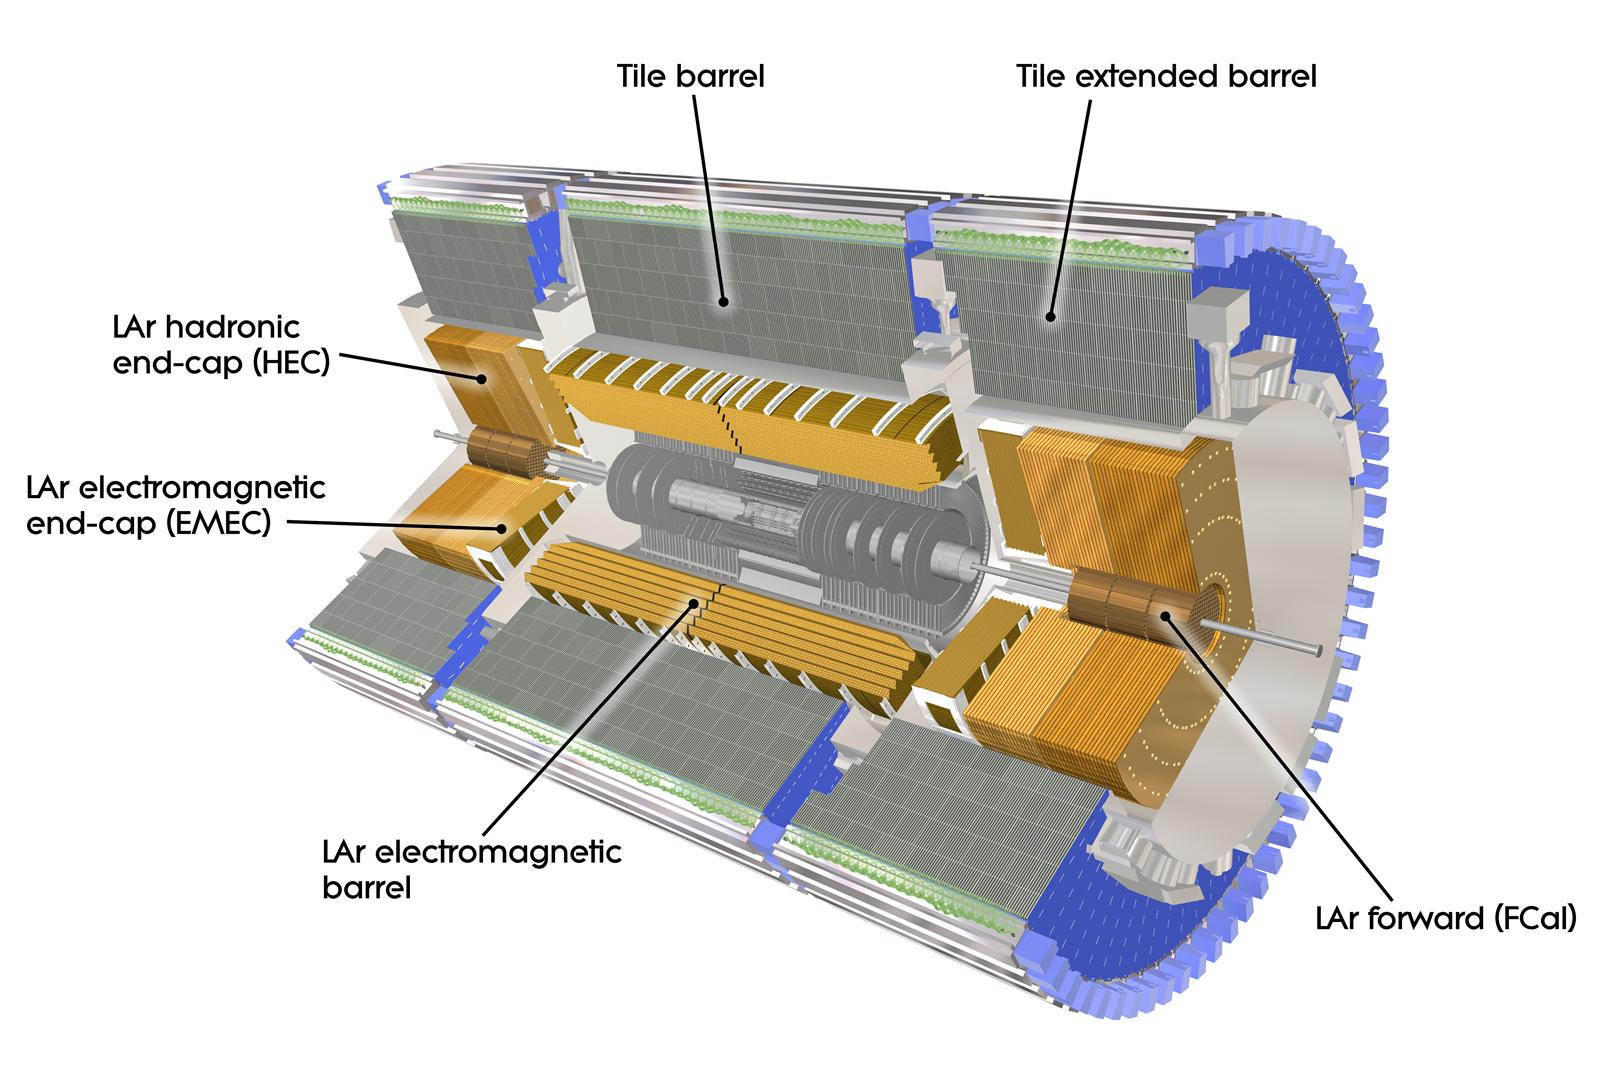
\includegraphics[width=0.8\textwidth]{chapters/2.detector/figs/atlas_calos.jpg}
  \caption{
    The \ATLAS calorimeters \cite{atlascalo}.
    The ECal uses LAr-based detectors, while the HCal uses mainly scintillating tile detectors.
    In the forward region the HCal also includes the LAr hadronic endcaps.
  }
  \label{fig:atlas_calos}
\end{figure}
%


\subsubsection{Liquid Argon (LAr) Electromagnetic Calorimeter}
The more granular lead/liquid-argon ECal covers the region $|\eta|< 3.2$ and is split into barrel (covering $|\eta| < 1.475$) and end-cap (covering $1.375 < |\eta| < 3.2$) regions.
EM calorimetry works by encouraging electrons and photons to interact with electrically charged particles in detector material via bremsstrahlung ($e \rightarrow e\gamma$) and pair production ($\gamma \rightarrow e^+ e^- $).
The EM calorimeter uses lead absorber plates to initiate EM showers, resulting in secondary particles which ionise the surrounding liquid argon.
The charge is collected on copper electrodes and read out.
The accordion geometry of the ECal allows for a full coverage in $\phi$ without any azimuthal cracks.

The energy resolution of the LAr calorimeter is made up of a sampling and a constant term, which are summed in quadrature to produce the overall energy resolution.
The sampling term contributes approximately $\pct{10} / \sqrt{E}$, while the constant term adds an additional \pct{0.7}.
Photons with moderate transverse energy $\ET \approx \SI{50}{\GeV}$ have an overall energy resolution of at most \pct{1.6} over most of the pseudorapidity range.
At lower $\ET \approx \SI{10}{\GeV}$, the resolution is degraded to approximately \pct{5}.
The resolution measurements are obtained from test beam data \cite{ATLAS-TDR-14}.

%it initiates an electromagnetic cascade,
%The fine granularity of the EM calorimeter
%Additionally, multiple samplings of the shower are used to resolve its pointing vector.

\subsubsection{Hadronic Tile Calorimeter}
In the central barrel region with $|\eta| < 1.7$, the HCal uses a tile calorimeter with steel as an absorbing material, and scintillating tiles as the active material.
Two copper/liquid-argon calorimeter end-caps are also used.
Incident hadrons interact via the strong and electromagnetic forces with the absorber material, mainly loosing energy due to multiple inelastic nuclear collisions.
The active material captures the resulting electrons and photons to measure the energy of the incident hadron.

The hadronic energy resolution of the HCal is parameterised as a function of the hadron's transverse energy
%
\begin{equation}
  \sigma(\ET) / \ET = \pct{50} / \sqrt{\ET} \oplus \pct{3} ,
\end{equation}
%
corresponding to a energy resolution of \pct{11} (\pct{6.5}) for a hadron with \ET of approximately \SI{10}{\GeV} (\SI{50}{\GeV}) \cite{ATLAS-TDR-03}.

%Hadrons are relatively massive and cannot radiate much of their energy through bremsstrahlung, and they lose their energy mainly through multiple nuclear collisions.  Hadrons passing through matter also initiate cascades through inelastic hadron-nuclei interactions.

%The tile calorimeter is placed directly outside the EM calorimeter envelope.o 
%The barrel covers the region -1.0<η<1.0, and the extended barrels cover the region 0.8<|η|<1.7.

%LAr hadronic end-cap calorimeter (HEC). Located directly behind (in $z$) the end-cap electromagnetic calorimeter and sharing the same LAr cryostats. The high level of radiation in the forward regions would cause severe damage to plastic scintillators. In the end-caps, parallel copper plates are submerged in liquid argon, which is preferred as the active medium because of its inherent radiation hardness.


\subsection{Muon Spectrometer}\label{sec:muon_spectrometer}

Due to their higher mass, muons easily pass unimpeded through the ID and calorimeters and therefore require specialised detectors for their measurement.
% higher mass means brem is less effective at slowing them down. though
The Muon Spectrometer (MS) is made up of dedicated tracking and triggering hardware, as shown in \cref{fig:atlas_muon_system}.
The precision tracking system uses three layers of monitored drift tubes with a barrel region covering $|\eta| < 1.2$ and end-caps covering $1 < |\eta| < 2.7$. The inner layers of the end-caps use cathode strip chambers to better cope with the high occupancy in the forward region.
The trigger system is comprised of resistive plate chambers in the barrel region covering $|\eta| < 1.0$ and thin gap chambers in the end-cap regions covering $1 < |\eta| < 2.4$.
A set of three superconducting air-core toroidal magnets, each made up of eight coils, is used in each of the barrel and end-caps to deflect the muons as the pass through the MS, allowing their momentum and charge to be measured from the direction and magnitude of curvature.
The toroidal magnets generate a field which is largely orthogonal to the muon trajectories which allows for maximum deflection.
The transverse momentum resolution (measured for combined ID and muon tracks, see \cref{sec:lepton_reco}) has been measured to be approximately \pct{1.7} in the central region for \lowpt muons, increasing to \pct{4} for \highpt muons in the forward regions \cite{Artoni:1953654}.
%
\begin{figure}[!htpb]
  \centering
  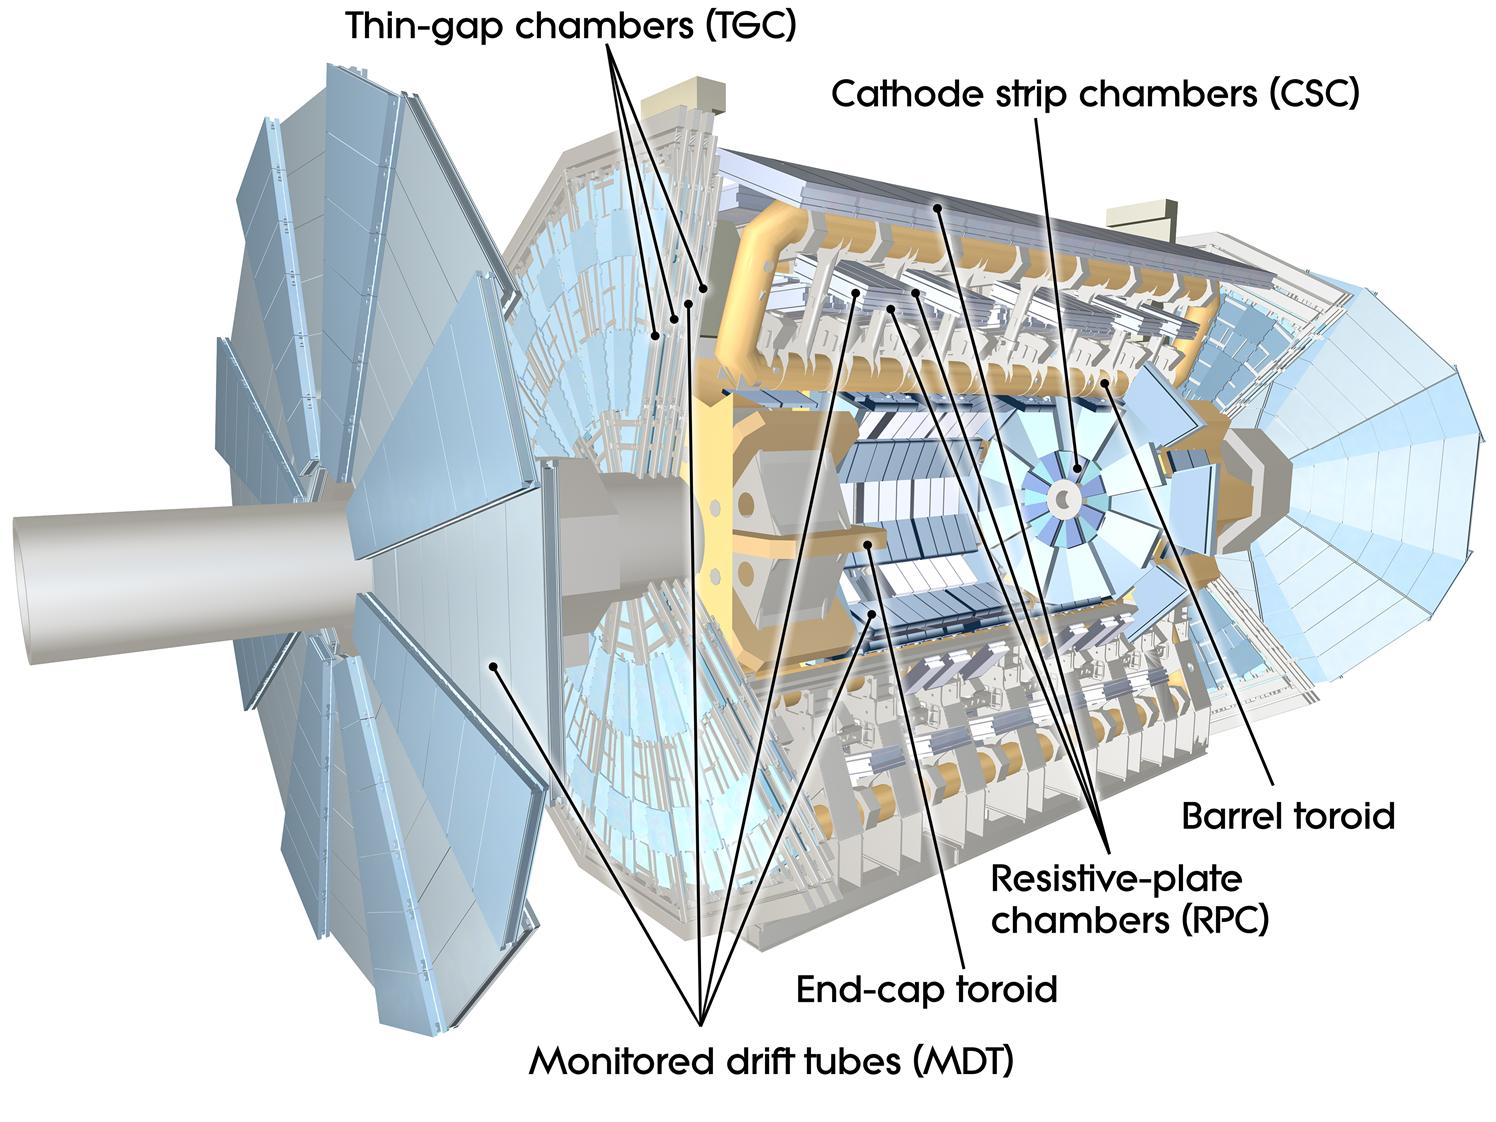
\includegraphics[width=0.7\textwidth]{chapters/2.detector/figs/atlas_muon_system.jpg}
  \caption{The \ATLAS muon spectrometer \cite{atlasmuon}.}
  \label{fig:atlas_muon_system}
\end{figure}
%


\subsection{The Trigger}\label{sec:trigger}
The \SI{25}{\nano\second} bunch spacing used over the course of \runtwo corresponds to a bunch-crossing or event rate of \SI{40}{\mega\hertz} (see \cref{tab:lhc_runs}).
If the full information for the detector was written out for each event, this would correspond to the generation of \SI{60}{\tera\byte} of data each second.
This is more than can be feasibly read out from the hardware, processed and stored, requiring the use of a trigger system which quickly makes a decision about whether or not an event is potentially interesting and should be kept for further analysis.
The trigger system is comprised of two levels which aim to identify various signatures, such as electrons, muons, taus, photons, and jets (including \bjets), as well as events with large total or missing transverse energy.
The hardware-based Level-1 (L1) trigger uses coarse information from the calorimeters and MS to accept events at an average rate of \SI{100}{\kilo\hertz} approximately \SI{2.5}{\micro\second} after the event.
After the L1 trigger, the software-based High Level Trigger (HLT) makes use of \num{40000} CPU cores to make a final selection on surviving events in approximately a few hundred milliseconds. 
The final event read-out rate is approximately \SI{1.2}{\kilo\hertz}, corresponding to \SI{1.2}{\giga\byte\per\second} of permenant data storage.
More information is provided in \cite{TRIG-2016-01}.
%Regions of Interest (ROIs) from the L1 trigger are used.

%The L1 trigger searches for high transverse-momentum muons, electrons, photons, jets, and $\tau$-leptons decaying into hadrons, as well as large missing and total transverse energy. Its selection is based on information from a subset of detectors. High transverse-momentum muons are identified using trigger chambers in the barrel and end-cap regions of the spectrometer. Calorimeter selections are based on reduced-granularity information from all the calorimeters. Results from the L1 muon and calorimeter triggers are processed by the central trigger processor, which implements combinations of different trigger selections. In each event, the L1 trigger also defines one or more Regions-of-Interest (RoI’s), i.e. the geographical coordinates in $\eta$ and $\phi$, of those regions within the detector where its selection process has identified interesting features. The RoI data include information on the type of feature identified and the criteria passed, e.g. a threshold. This information is subsequently used by the high-level trigger.

%The L2 selection is seeded by the RoI information provided by the L1 trigger. L2 selections use, at full granularity and precision, all the available detector data within the RoI’s (approximately 2\% of the total event data). The L2 menus are designed to reduce the trigger rate to approximately 3.5 kHz, with an event processing time of about 40 ms, averaged over all events. The final stage of the event selection is carried out by the event filter, which reduces the event rate to roughly 200 Hz. Its selections are implemented using offline analysis procedures within an average event processing time of the order of four seconds.










\section{Reconstructed Physics Objects}\label{sec:physics-objects}

Event reconstruction is the process of analysing the output from the detector to determine the type and properties of particles present in an event. 
The reconstructed event provides information about the underlying physics process that led to these observable final state particles.
Events passing the trigger selection (described in \cref{sec:trigger}) undergo offline reconstruction, which makes use of the full information from the detector.
Reconstruction and analysis of events relies on the extensive \ATLAS software stack, see \rcite{ATL-SOFT-PUB-2021-001} for more information.

Several different reconstructed objects are used for physics analyses.
Objects relevant to this thesis are described below.



\subsection{Tracks}\label{sec:track_reco}
% diagram at 
% https://atlassoftwaredocs.web.cern.ch/trackingTutorial/idoverview/
The reconstructed trajectories of charged particles are referred to as \textit{tracks}.
Tracks are reconstructed from the energy depositions (called \textit{hits}) left by the particles as they traverse the inner detector.
Tracks are used in the reconstruction of other objects, including vertices and jets, so their accurate reconstruction is a critical task.
A comprehensive introduction to ATLAS tracking is available in \rcite{Cornelissen:2007vba}, while specific optimisations for dense environments are detailed in Refs.~\cite{ATL-PHYS-PUB-2015-006, PERF-2015-08}.
An overview of track reconstruction is given below.

%Tracking is useful for: impact parameter measurements, vertexing for heavy-flavour and $\tau$ tagging.

\subsubsection{Space-point Formation (Clustering)}
When a charged particle traverses a silicon layer, charge can be collected in more than one pixel or strip.
This is due to the incident angle of the particles with respect to the sensor, and also the drift of electrons between sensors caused by the magnetic field.
Clusters (also called \textit{hits} or \textit{space-points}) are formed by clustering neighbouring pixels or strips and estimating locations of space-points using the shape and energy distribution of the clusters.

\subsubsection{Track Finding}
Space-points are used to build track seeds. These are groups of three hits which are geometrically compatible with being part of a track segment.
A combinatorial Kalman filter (KF) is used to build track candidates by extending track seeds.
The filter can create multiple track candidates per seed, with bifurcations along the track occurring when more than one compatible space-point exists on a given layer.
In this way, the KF creates an excess of \textit{track candidates}, which are only required to satisfy basic quality requirements. 
Track candidates are allowed to reuse or \textit{share} hits freely (a single hit may be used by multiple track candidates).
Typically, the presense of shared hits is a predictor of a bad track due to the high granularity of the ATLAS tracking detectors.
At this stage, there can also be a large number of incorrect hits assigned to otherwise good tracks, and additionally large numbers of \textit{fake} tracks, which are comprised of a majority of wrong hits and do not correspond to the trajectory of any one physical particle (fake tracks are defined as those where the majority of associated hits do not originate from one single truth particle, see \cref{eq:tmp_def}).
The low quality of tracks at this stage necessitates an ambiguity solving step, in which candidates are cleaned, and the highest quality track are selected.

\subsubsection{Ambiguity Solving}
Ambiguity solving was introduced as part of the ATLAS New Tracking effort \cite{Cornelissen:2007vba}, which was intended to improve track reconstruction performance in dense environments.
In the ambiguity solver, track candidates are processed individually in descending order of a track score. The track score quantifies the likelihood of the track corresponding to the trajectory of a real particle. Scoring uses a number of variables, including the number and positions of hits (preferring hits in more precise regions of the detector), the transverse momentum of the track and the track fit quality. The track fit quality describes the quality of the track as the $\chi^2$ divided by the number degrees of freedom on the track. A preference for high transverse momentum tracks promotes the successful reconstruction of the more physically interesting energetic particles, and suppresses the large number of wrong hits assigned to low momentum tracks.
The ambiguity solver also penalises tracks with missing hits on the innermost detector layers. 

During the processing of a track candidate, the track is cleaned (whereby problematic hits are removed), and, if the resulting track satisfies the quality selection criteria, a high precision fit of the track parameters using the surviving hits is performed.
The high precision fit makes full use of all available information, and uses an updated position and uncertainty estimate for each cluster obtained from a Neural Network (NN) \cite{PERF-2012-05}.
If the track has reached this stage without being rejected by passing various quality requirements, it is re-scored and returned to the list of track candidates.
If the same track is then processed again without requiring modification, it is added to the final track collection.
Track candidates that fall below certain quality threshold are rejected.
This selection does allow for the possibility of a track having small number of shared hits, as detailed in \cref{tab:fake_track_mva_selections}.

\begin{table}[!htbp]
  \footnotesize\centering
  \setlength{\tabcolsep}{0.5em} % for the horizontal padding
  \begin{tabular}{ll}
    \toprule\hline
    \textbf{Parameter} & \textbf{Selection} \\
    \hline
    $\pt$                & $> 500$ MeV \\
    $|\eta|$             & $<2.5$ \\
    $|\dzero|$           & $< 3.5$ mm \\
    $|\zzero\sin\theta|$ & $< 5$ mm \\
    Silicon hits         & $\ge 8$ \\
    Shared silicon hits  & $< 2$ \\
    Silicon holes        & $< 3$ \\
    Pixel holes          & $< 2$ \\
    \hline\bottomrule
  \end{tabular}
  \caption{
    Quality selections applied to tracks,
    where \dzero is the transverse IP of the track, \zzero is the longitudinal IP with respect to the PV and $\theta$ is the track polar angle (see \cref{sec:track_parameterisation} for the IP definitions).
    Silicon hits are hits on the pixel and SCT layers.
    Shared hits are hits used on multiple tracks which have not been classified as split by the cluster-splitting neural networks~\cite{PERF-2015-08}.
    %Shared hits on pixel layers are given a weight of 1, while shared hits in the SCT are given a weight of 0.5.
    A hole is a missing hit, where one is expected, on a layer between two other hits on a track.
    }% https://twiki.cern.ch/twiki/bin/view/AtlasProtected/TrackingCPRecsRun2R22#Selection_Criteria
  \vspace{4mm}
  \label{tab:fake_track_mva_selections}
\end{table}


\subsubsection{Neural Network Cluster Splitting}
As part of track cleaning, shared hits are classified by a NN to determine if they are compatible with the characteristic features of a merged cluster \cite{PERF-2012-05, ATL-PHYS-PUB-2015-006}.
A merged cluster is one made up of a combination of energy deposits from more than one particle, which have become merged due to the closeness of the associated particles and the limited resolution of the detector.
It is common for clusters to become merged in dense environments, as discussed in \cref{sec:b_had_reco}.
If the cluster is predicted to be merged it is labelled as being freely shareable, or \textit{split}.
Hits not compatible with the merged hypothesis can still be shared by a limited number of tracks, but come with a penalty for the track which may hinder its acceptance into the final track collection.
%
\begin{figure}[ht]
    \centering
    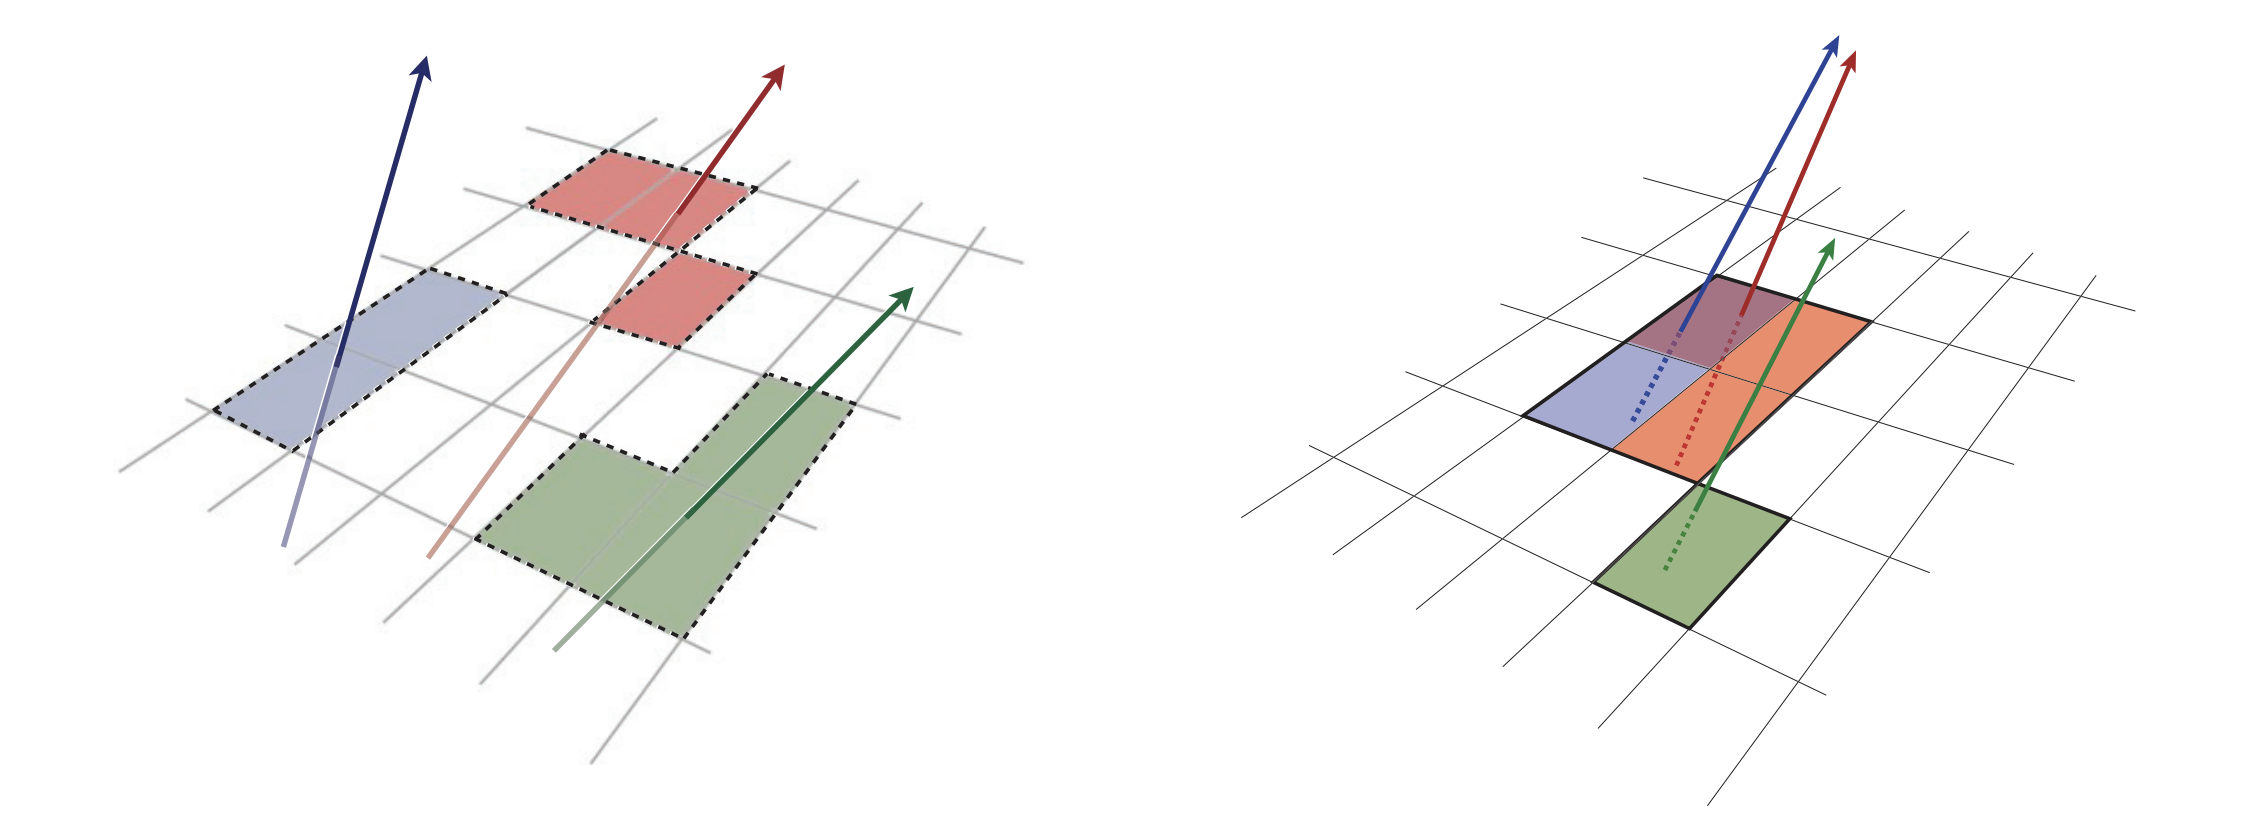
\includegraphics[width=0.8\textwidth]{chapters/2.detector/figs/merged-cluster.png}
    \caption{
      Particles (left) which have enough separation will leave charge depositions which are resolved into separate clusters.
      Sufficiently close particles (right) can lead to merged clusters.
      Their combined energy deposits are reconstructed as a single merged cluster \cite{PERF-2015-08}.}
    \label{fig:resolved/merged clusters}
\end{figure}
%

\subsubsection{Pseudotracking}\label{sec:pseudotracks}

Pseudotracking uses Monte Carlo truth information to group together all the hits left by each truth particle.
Each collection of hits which, as a unit, satisfies basic quality requirements is directly used in a full resolution track fit.
If the track fit is successful, a ``pseudotrack'' track is created and stored.
If the track fit fails, or the collection of hits does not pass the basic quality requirements (for example because of a lack of hits) then the particle is said to be un-reconstructable.
In this way, pseudotracking performance represents the ideal reconstruction performance given the ATLAS detector, with perfect hit-to-track association and track reconstruction efficiency.
The approach was introduced in \rcite{Jansky:2013ryb} as a way to obtain a fast approximation of tracking reconstruction for simulated data, however the technique has become a useful tool for studying tracking performance in general \cite{ATL-PHYS-PUB-2015-006}.


\subsection{Vertices}\label{sec:vertex_reco}
Groups of reconstructed tracks can be examined to determine whether the particles originated from a common spatial point of origin.
This occurs when proton-proton collisions take place (primary vertices), when a particle decays or radiates, and also as a result of interaction with the detector material (secondary vertices).
Vertex reconstruction is made up of two stages.
First, vertex finding takes place, which is the process of grouping tracks into compatible vertices.
Second, vertex fitting combines information from compatible tracks to reconstruct the physical properties of the vertex, such as mass and position.

\subsubsection{Primary Vertices}
Each proton-proton interaction happens at a \textit{primary vertex} (PV).
Primary vertices are iteratively reconstructed with tracks using the iterative vertex finder (IVF) \cite{PERF-2015-01}.
%In \runthree, the IVF will be replaced with an adaptive multi-vertex finder (AMVF) \cite{ATL-PHYS-PUB-2019-015}.
The \textit{hard scatter vertex} of an event is chosen as the primary vertex whose associated tracks have the largest sum of transverse momentum squared, $\Sigma(\pt^2)$.

\subsubsection{Secondary Vertices}
Secondary vertices (SV) occur when a particle radiates or decays at a sufficient distance from the primary vertex to be resolved from the primary vertex (see \cref{sec:b_decay_topology}).
Two widely used secondary vertexing tools are used within \ATLAS: SV1 and JetFitter \cite{FTAG-2018-01,ATL-PHYS-PUB-2017-011}.
Each attempts to reconstruct secondary vertices inside a jet using the tracks associated to that jet (see \cref{sec:jet_reco} for more information about track association).
SV1 by design attempts to reconstruct only a single inclusive vertex per jet.
This inclusive vertex groups all \bhadron decay products, including tracks from the \bhadron decay itself and tracks from $b \rightarrow c$ decays.
The second tool, JetFitter attempts to resolve each displaced vertex inside the jet, such that secondary vertices from \bhadron decays are reconstructed separately to tertiary vertices from $b \rightarrow c$ decay chains.


\subsection{Jets}\label{sec:jet_reco}
Jets are an aggregate reconstructed object corresponding to a collection of collimated stable particles which results from the presence of a quark or gluon.
Jets are built by clustering constituent objects (e.g. tracks or calorimeter clusters) using a jet finding algorithm, for example the \antikt algorithm \cite{Cacciari:2008gp}, which is implemented in \textsc{FastJet}~\cite{Cacciari:2012:fastjet}.

Objects can be associated to jets in one of two ways.
The first is via a geometrical matching in $\DeltaR$ (see) 
The second is via a ghost association \cite{Cacciari:2008gn}, where the object is assigned a negligible momentum and re-clustered into the jet after its formation.

Jets from pile-up interactions are suppressed using the Jet Vertex Tagger (JVT) algorithm, which uses the transverse momenta of tracks to identify jets from pile-up interactions \cite{ATLAS-CONF-2014-018}.



\subsubsection{EMTopo Jets}
EMTopo jets are reconstructed from noise-suppressed topological clusters (topoclusters) of calorimeter energy depositions \cite{PERF-2014-07}.
The clustering uses the energy significance of each cell, defined as 
%
\begin{equation}
  S_\textnormal{cell} = \frac{E_\textnormal{cell}}{\sigma_\textnormal{noise, cell}} ,
\end{equation}
%
where $E_\textnormal{cell}$ is the energy measured in a given calorimeter cell, and $\sigma_\textnormal{noise, cell}$ is the expected level of noise on the cell (e.g. from pile-up interactions).
Topoclusters are formed from a seed cell with a large $S_\textnormal{cell}$, and expanded by iteratively adding neighbouring cells with a sufficiently large energy significance.
Collections of topoclusters are then clustered into a jet 
using the \antikt algorithm with a radius parameter of $0.4$ (\smallR jets) or $1.0$ (\largeR jets).
More information, including information on the calibration of the topocluster jet energy scale, is available in \rcite{PERF-2014-07}.


\subsubsection{Particle Flow Jets}
Particle-flow (PFlow) jets are reconstructed from particle-flow objects \cite{PERF-2015-09} using the \antikt algorithm with a radius parameter of $0.4$.
Particle-flow objects integrate information from both the ID and the calorimeters, improving the energy resolution at high transverse momenta and reducing pile-up contamination.
The PFlow jet energy scale is calibrated according to \rcite{PERF-2016-04}.

\subsubsection{\texorpdfstring{\LargeR}{Large-R} Jets}
\LargeR jets have a radius parameter $R=1.0$ and are built by clustering topological calorimeter clusters using the \antikt algorithm \cite{Butterworth:2008iy}.
The large radius parameter is especially useful for containing the decay products of a boosted Higgs boson, as discussed in \cref{chap:vhbb_boosted}. 
Due to their large size, \largeR jets benefit from a grooming procedure called trimming which remove soft contaminants inside the jet \cite{ATLAS:2020jwz,ATLAS:2013bqs}.
Trimming aims to remove jet constituents from pile-up and the underlying event, which helps to improve the jet mass resolution and its robustness to varying levels of pile-up.
The jet mass is computed using a combination of information from the calorimeters and ID, and a calibration to data is applied \cite{JETM-2018-02}.


\subsubsection{Track-jets}
Track-jets are built by clustering tracks using the \antikt clustering algorithm.
They are associated to \largeR jets as sub-jets and used to identify \largeR jets containing \bhadrons.
The radius parameter is allowed to vary with transverse momentum such that a broader cone (up to $R=0.4$) is used for \lowpt track-jets and a narrower cone (down to $R=0.02$) for \highpt track-jets \cite{Krohn:2009zg,ATL-PHYS-PUB-2017-010}.
The narrower cone is better suited to clustering highly collimated jet constituents at \highpt.

\subsubsection{Jet Flavour Labels}
Jet flavour labels are assigned to \smallR jets according to the presence of a truth hadron within ${\DeltaR(\text{hadron},\text{jet})<0.3}$ of the jet axis. If a \bhadron is found the jet is labelled a \bjet. In the absence of a \bhadron, if a \chadron is found the jet is called a \cjet.
If no \borchadrons are found, but a $\tau$ is found in the jet, it is labelled as a $\tau$-jet, else it is labelled as a \ljet.
%Jet flavour labels are assigned according to the presence of a truth hadron within ${\DeltaR(\text{hadron},\text{jet})<0.3}$ of the jet axis. If a \bhadron is found the jet is labelled a \bjet. In the absence of a \bhadron, if a \chadron is found the jet is called a \cjet.
%If no \borchadrons are found, but a $\tau$ is found in the jet, it is labelled as a $\tau$-jet, else it is labelled as a \ljet.

PFlow jets are used to train the algorithms discussed in \cref{chap:track_classification_mva} and \cref{chap:gnn_tagger}.

\subsubsection{Jet Track Association}
Tracks are associated to \smallR jets using a \DeltaR association cone, the width of which decreases as a function of jet \pt, with a maximum cone size of $\DeltaR \approx 0.45$ for jets with $\pt = \SI{20}{\GeV}$ and minimum cone size of $\DeltaR \approx 0.25$ for jets with $\pt > \SI{200}{\GeV}$. 
If a track is within the association cones of more than one jet, it is assigned to the jet which has a smaller $\DeltaR(\text{track}, \text{jet})$.


\subsection{Leptons}\label{sec:lepton_reco}

Electrons and muons leave characteristic signatures that are picked up in the ECal and MS respectively.
The reconstruction of both types of charged lepton is briefly outlined below.

\subsubsection{Electrons}

A diagrammatic view of electron reconstruction is shown in \cref{fig:electron_Reco}.
Electrons candidates are reconstructed by matching PV-compatible\footnote{The ID track associated with the electron is required to satisfy $\dzero / \dzerosig < 5$ and $\zzero\sin\theta < \SI{0.5}{\milli\meter}$.} inner detector tracks to topological calorimeter clusters.
The track-cluster matching criteria takes into account the significant energy loss of the electron due to bremsstrahlung.
If a match is found, a refit of the track is performed using the Gaussian Sum Filter (GSF) \cite{ATLAS-CONF-2012-047}, which better handles trajectory reconstruction in the presence of bremsstrahlung.
Various identification criteria are then applied to the candidates using a likelihood-based (LH) method to improve purity.
These include requirements on the track quality and cluster matching, the shape of electromagnetic shower in the ECal, leakage into the HCal, and the amount of transition radiation detected in the TRT.
Isolation criteria with respect to other nearby ID tracks and calorimeter clusters may also be applied.
A full description can be obtained from \rcite{ATLAS-CONF-2016-024}.
%
\begin{figure}[!htbp]
  \centering
  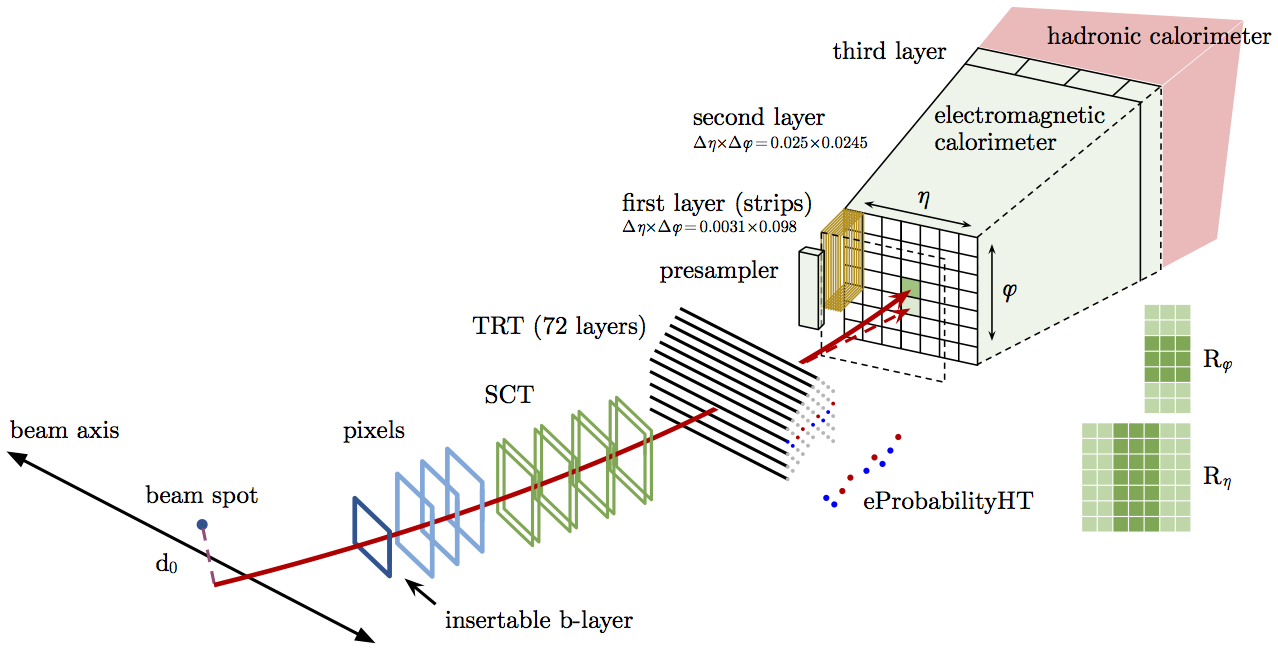
\includegraphics[width=0.8\textwidth]{chapters/2.detector/figs/electron_reco.png}
  \caption{
    A sketch of electron reconstruction using the \ATLAS detector \cite{ATLAS-CONF-2016-024}.
    Electron reconstruction makes use of the entire ID and the calorimeters.
    %In particular, discriminating information comes from the TRT and ECal.
  }
  \label{fig:electron_Reco}
\end{figure}
%


\subsubsection{Muons}
Muon reconstruction makes use of the dedicated MS (see \cref{sec:muon_spectrometer}), the tracks from the ID, and the presence of characteristic signatures in the calorimeters.
Muon tracks (i.e. a track reconstructed in the MS) are reconstructed by connecting straight-line track segments, which are identified via a Hough transform, and combined into a approximately parabolic trajectory.
Finally, a global $\chi^2$ fit is performed, taking into account possible interactions between the muon and the detector material.
A reconstructed muon is called \textit{combined} if it can be matched successfully to an to an ID track.
Combined muons undergo a further fit with the combined ID and MS hits, with the energy loss due to the traversal of the calorimeters being taking into account.

After reconstruction, candidate undergo an identification processes which helps to efficiently identify prompt muons whilst rejecting background signals (e.g. non-prompt muons from pion and kaon decays, the punch-through of a hadron from the calorimeter, or the semi-leptonic decay of a heavy flavour hadron).
Combined muon identification takes into account discrepancies in the \pt and charge measurements in the MS and ID, and the $\chi^2$ of the combined track fit.
Selections on the number of hits in the ID and MS are also applied.
At the medium identification working point, approximately \pct{96} of prompt muons with $\SI{20}{\GeV} < \pt < \SI{100}{\GeV}$ are successfully identified.
On top of the identification requirements, a number of isolation requirements can also be applied to further suppress background signals.
%In the region $|\eta| < 2.2$, the momentum resolution of reconstructed muons is \pct{1.7}.

More information on muon reconstruction, identification and isolation can be found in \rcite{PERF-2015-10}.


\subsection{Missing Transverse Momentum}\label{sec:missing_Et}

An imbalance in the final state transverse momentum can occur as a result of incomplete measurement of the final state particles.
In particular, neutrinos are not measured by the detector and contribute to the missing transverse momentum \vETmiss.
Incomplete detector acceptance and inaccuracies in the reconstruction of the final state can also contribute to the missing transverse momentum of an event.
In order to calculate the missing transverse momentum, the negative vector sum of the momentum of all photons, leptons and \smallR jets with $\pt > \SI{20}{\GeV}$ is taken.
The momenta of tracks associated to the primary vertex are also taken into account.
The magnitude of \vETmiss is written \ETmiss.
More information about missing transverse momentum reconstruction is provided in \cite{PERF-2016-07}.

  \chapter{Tracking and Flavour Tagging at High-\texorpdfstring{\pt}{pt}}\label{chap:tracking}

The various flavour tagging algorithms introduced in \cref{sec:btagging_algs} work by identifying the unique signatures of heavy flavour jets ($b$- and \cjets).
Ultimately, the tagging algorithms use input information about the reconstructed jet and its associated tracks.
Successful \btagging therefore relies on the efficient and accurate track reconstruction, especially for tracks corresponding to the products of heavy flavour decays.
In this chapter the challenges facing track reconstruction and flavour tagging at \highpt are discussed.


The chapter is structured as follows.
In \cref{sec:track_classifier_datasets} an introduction to the datasets used in this thesis is given.
A summary of the challenges facing tracking and \btagging at high transverse momentum is provided in \cref{sec:b_had_reco_chall}.
Some preliminary investigations into improving tracking in the \highpt regime are investigated in \cref{sec:b_track_reco_improvements}.
Finally, in \cref{sec:trk_btag_conclusion} the conclusions of the chapter are given.


\section{Datasets}\label{sec:track_classifier_datasets}


\newcommand{\hdampFootnote}{%
The first gluon emission cut-off scale parameter $h_\text{damp}$ of the \textsc{PowhegBox} generator is used to limit the effect of resummed higher order corrections.%
It is used to suppress the transverse momentum of the radiation which the \ttbar system recoils against.%
}

This thesis makes extensive use of two simulated datasets which are described in this section.
The datasets are made up of simulated SM \ttbar and BSM \Zprime events\footnote{The \Zprime boson used in this thesis is a modified SM \Zboson with an increased mass} initiated by proton-proton collisions at a center of mass energy $\sqrt{s} = \SI{13}{\TeV}$.
While the \ttbar sample populates the \lowpt phase space, the \Zprime sample is constructed in such a manner that it has a relatively flat jet \pt spectrum up to \SI{5}{\TeV} and decays democratically to equal numbers of \bcl jets.
As a result, the \Zprime sample is well suited to the study of \btagging at \highpt.
The simulation includes the effect of multiple proton-proton interactions per bunch crossing with an average pile-up of $\langle \mu \rangle = 40$.
The effect on the detector response due to interactions from bunch crossings before or after the one containing the hard interaction are also included.

%effectively regulating the %
%is a resummation damping factor and one of the parameters that controls the matching of \textsc{Powheg} matrix elements to the parton shower and thus effectively regulates the %high-$p_T$ radiation against which the \ttbar system recoils.}

For the \ttbar sample, events are generated using the \textsc{PowhegBox}~\textsc{v2} generator~\cite{powheg2004, powheg2007, powheg2007_2, powheg2010} at next-to-leading order in the strong coupling constant $\alpha_s$.
The NNPDF3.0NNLO \cite{Ball:2014uwa} set of parton distribution functions (PDFs) are used for the calculation of the hard scatter matrix element.
The $h_\text{damp}$ parameter\footnote{\hdampFootnote} is set to 1.5 times the mass of the top-quark~\cite{ATL-PHYS-PUB-2016-020}, with $m_\text{top} = \SI{172.5}{\GeV}$.
The simulated hard scatter events are interfaced with \textsc{Pythia}~8.230~\cite{Sjostrand:2014zea} using the A14 parameter tune and the NNPDF2.3LO PDFs to handle the simulation of the parton shower, hadronisation, and underlying event.
These choices were found to best model the top quark transverse momentum and the number of additional jets in the event \cite{ATL-PHYS-PUB-2016-020,ATL-PHYS-PUB-2020-023}.
Meanwhile for the \Zprime sample, full events are generated with \textsc{Pythia}~8.212.
Again, the A14 tune \cite{ATL-PHYS-PUB-2014-021} and the NNPDF2.3LO set of PDFs \cite{Ball:2012cx} are used.

For both samples the decays of \bchadrons are performed by \textsc{EvtGen} v1.6.0 \cite{Lange:2001uf}.
After event generation, simulated particles are passed through the full ATLAS detector simulation \cite{SOFT-2010-01} which is based on GEANT4 \cite{Agostinelli:2002hh}.
The interaction between the long-flying heavy flavour hadrons and the detector material is included in the simulation.

Additional jet requirements are as follows.
Jets are required to have a pseudorapidity $|\eta| < 2.5$ and $\pt > \SI{20}{\GeV}$.
Jets are also required not to overlap with a prompt generator-level electron or muon from \Wboson boson decays.
Finally, a standard selection using the JVT tagger (see \cref{sec:jet_reco}) at the tight working point is applied to jets with $\pt < \SI{60}{\GeV}$ and $|\eta| < 2.4$ in order to suppress pile-up contamination \cite{ATLAS-CONF-2014-018}.



\section{\texorpdfstring{\bhadron}{b-hadron} Reconstruction Challenges}
\label{sec:b_had_reco_chall}

%This section some of the difficulties in the accurate reconstruction of the  associated reconstruction difficulties in \cref{sec:b_had_reco_chall}.
As discussed in \cref{sec:b_decay_topology}, a necessary requirement for successful \btagging is the efficient and accurate reconstruction of the charged particle trajectories in the jet.
For high \pT jets (\pT $> 250$ GeV) this task becomes difficult due to difficulties in the accurate reconstruction of tracks, as described below.

As the \bjet energy increases, the multiplicity of the fragmentation products inside the jet increases, while the multiplicity of the products of the weak decay remains fixed.
The ``signal'' tracks (those from the weak decay of the \bhadron) therefore become significantly outnumbered.
Both fragmentation and \bhadron weak decay products also become increasingly collimated as their inherited transverse momentum increases.
This is compounded by the increased decay length of \bhadrons (and \chadrons) at \highpt, which means that the decay products have less of an opportunity to diverge before reaching the first tracking layers of the detector (shown in \cref{fig:high_pt_b_decay}).
If the weak decay of the \bhadron takes place close enough to a detector layer, or if the particles are otherwise sufficiently collimated, charge deposits left by nearby particles may not be resolved individually, instead being reconstructed as merged clusters \cite{PERF-2015-08}.

\begin{figure}[!htbp]
  \centering
  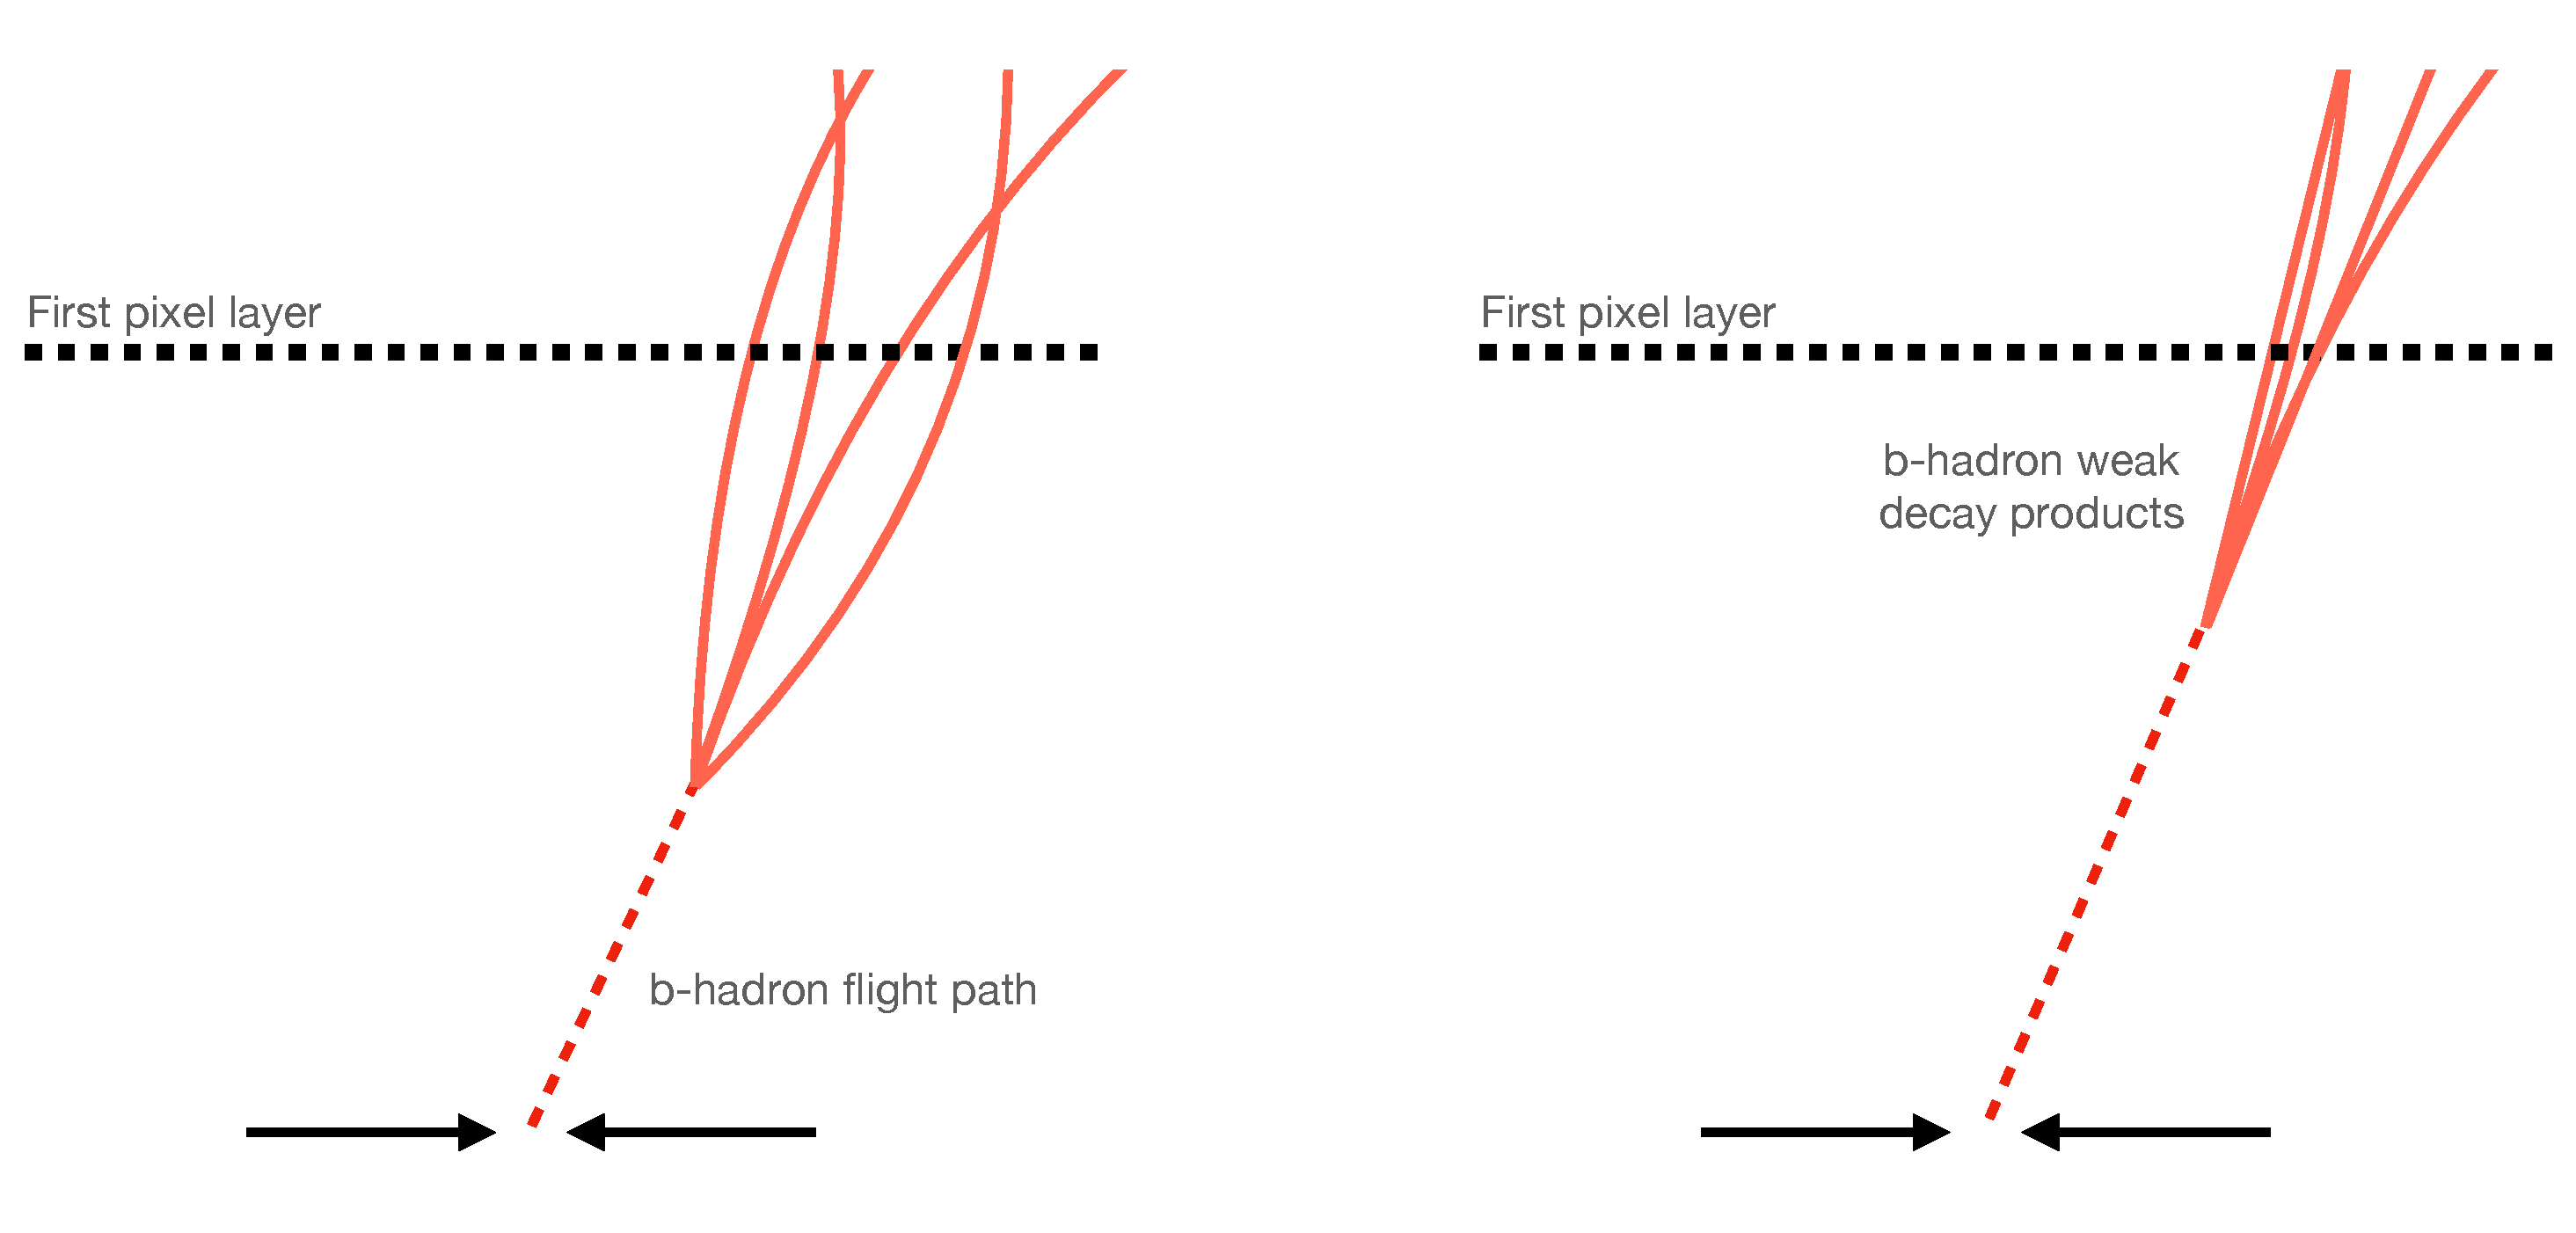
\includegraphics[width=0.8\textwidth]{chapters/3.tracking/figs/high_pt_b_decay.pdf}
  \caption{
    At lower \pt (left) the decay length of the \bhadron is on average reduced, and the decay tracks are less collimated.
    At higher \pt (right) the \bhadron decay length increases and the resulting decay tracks are more collimated and have less distance over which to diverge before reaching detector elements.
    As a result, the ID may be unable to resolve charged depositions from different particles, resulting merged clusters.
  }
  \label{fig:high_pt_b_decay}
\end{figure}

As discussed in \cref{sec:track_reco}, merged clusters are generally rare, and so shared hits generally predict bad tracks and are correspondingly penalised during track reconstruction.
However, in the core of high \pT \bjets the density of particles is high enough that the probability of cluster merging increases dramatically.
Successful reconstruction of such tracks requires the presence of shared hits to be effectively dealt with, but in the standard reconstruction the presence of these can instead impair the successfully reconstruction of the track.
Furthermore, heavy flavour decays may also take place inside the tracking detectors themselves, which at best leads to missing measurements on the most sensitive detector layers, and at worst can lead to wrong inner layer hits being added to displaced tracks, since the reconstruction process penalises tracks without inner layer hits.

%Together, these two effects lead to a high density of charged particles in the jet core, which, given the finite resolution of the detector, makes reconstruction difficult.




\begin{comment}
%
\begin{figure}[!htbp]
    \centering
    %\includegraphics[width=\textwidth]{res/figs/results/tracking/b-reco-efficiency.png}
    \vspace{0.05em}
    \caption{Track reconstruction efficiency from \bhadron decay products for baseline ATLAS tracking (black), Bcut+Refit procedures applied (green), pseudo-tracking (blue), and for tracking where the ambiguity solver has been manually removed (orange).}
    %The relatively high reconstruction efficiency at the stage of the track candidates (i.e. before ambiguity solving) indicates that the efficiency loss is driven by the ambiguity solver.
    \label{fig:reconstruction efficiency from B}
\end{figure}

\begin{figure}[!htbp]
    \centering
    %\includegraphics[width=\textwidth]{res/figs/results/tracking/po_nHitsOnPix_From_B_DL.pdf}
    \vspace{0.05em}
    \caption{The total number of pixel hits on tracks from \bhadron decays as a function of the production radius of the decay product. An excess of hits is assigned to the standard tracks in comparison to the ideal pseudotracks.}
    \label{fig:total hits on pix from b}
    \label{fig:misc}
\end{figure}
%
\end{comment}


The above effects create two distinct but related  problems for \btagging.
The first is a drop in track reconstruction efficiency.
%As mentioned, tracks originating from high energy \bhadron decay products can have a high rate of shared hits due to the number of particles present in a high \pT \bjet and their relative collimation.
%Additionally, tracks may be missing hits on the inner layers of the detector in the case of displaced decays.
The presence of shared and missing hits reduces a track's score in the ambiguity solver meaning that higher ranking, but potentially less accurate, track candidates are processed first and take ownership of the hits.
This can make it difficult for otherwise reasonable \bhadron decay tracks to meet the ambiguity solver's stringent track quality requirements, leading to their rejection at this stage and an overall decrease in the \bhadron decay track reconstruction efficiency.
As shown in \cref{fig:b_track_eff}, this can result in a large drop in reconstruction efficiency for \bhadron decay products of up to \pct{50} for at $\pt > \SI{2}{\TeV}$.

\begin{figure}[!htbp]
  \centering
  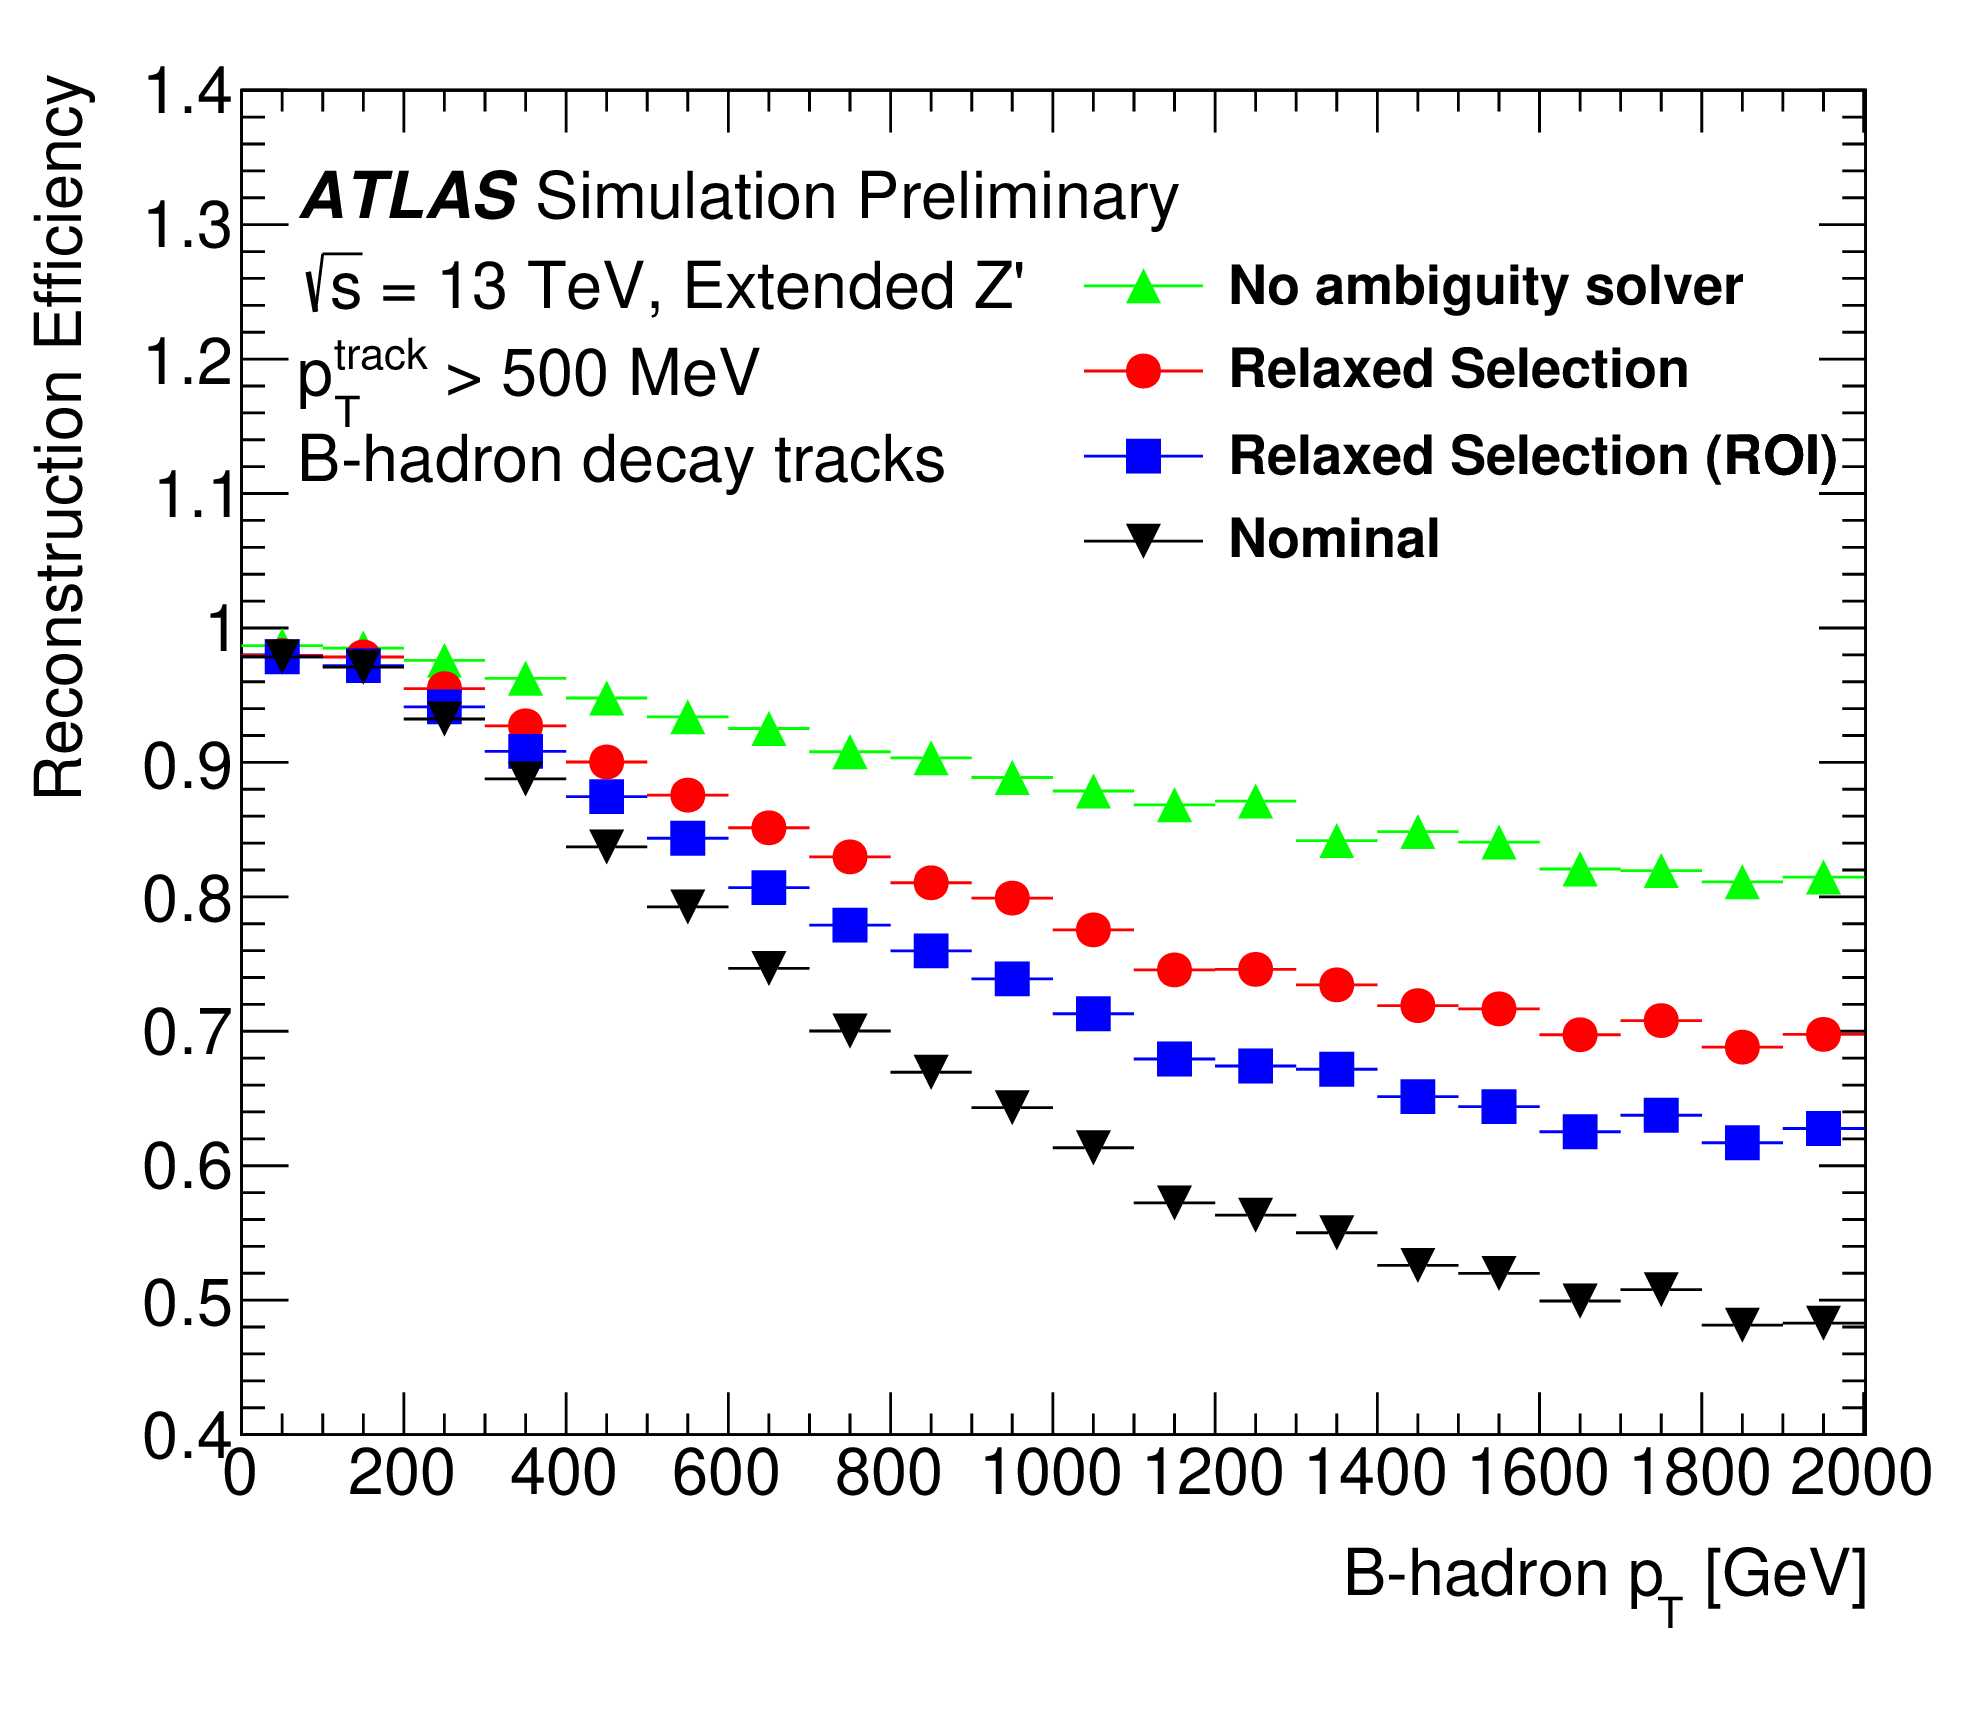
\includegraphics[width=0.6\textwidth]{chapters/3.tracking/figs/b_track_reco_eff.png}
  \caption{
    \bhadron decay track reconstruction efficiency as a function of truth \bhadron \pt for \Zprimejets \cite{2022DonalTrackReco}.
    Nominal track reconstruction is shown in black, while the track reconstruction efficiency for track candidates (i.e. the pre-ambiguity solver efficiency) is shown in green.
    For \highpt \bhadrons, the ambiguity solver is overly aggressive in its removal of \bhadron decay tracks.
    Suggestions for the improvement of the track reconstruction efficiency in this regime by the loosening of cuts in the ambiguity solver are shown in blue and red.
  }
  \label{fig:b_track_eff}
\end{figure}

%As a result, many B decay tracks are rejected in the ambiguity solving stage, leading to a severe drop in tracking reconstruction efficiency. This is shown by the severe decrease in reconstruction efficiency visible when comparing baseline tracking with the ideal pseudotracks in \cref{fig:reconstruction efficiency from B}. This situation presents a problem: relaxing cuts on shared hits significantly degrades the ambiguity solver's power to reject bad tracks. However for \bhadron decay tracks it seems these same restrictions on shared hits are seriously impairing the reconstruction efficiency of good tracks. 

The second part of the problem is that, due to the high multiplicity of clusters available for assignment in the vicinity of the typical \highpt \bhadron decay track, and also given the strong positive bias of the ambiguity solver towards those tracks with pixel measurements in each layer (especially the innermost IBL measurement), many \bhadron decay tracks are assigned incorrect inner layer hits.
This is only a problem for those decay products which were produced within the pixel detector as a result of a significantly displaced \bhadron decay, and so do not have a correct hit available for assignment.
\cref{fig:pseudo_pix_hits} shows the number of hits as a function of the reconstructed track \pt for fragmentation tracks and tracks from the weak decay of the \bhadron.
The baseline tracks represent the standard reconstruction setup, while the pseudotracks represent the ideal tracking setup as outlined in \cref{sec:pseudotracks}.
Hit multiplicities on the pseudotracks decrease with increasing \pt due to the flight of the \bhadron before its decay. 
The baseline tracks have more hits than the pseudotracks, indicating that they are being incorrectly assigned additional hits on the inner layers of the detector.

\begin{figure}[!htbp]
  \centering
  \begin{subfigure}{.48\textwidth}
    \centering
    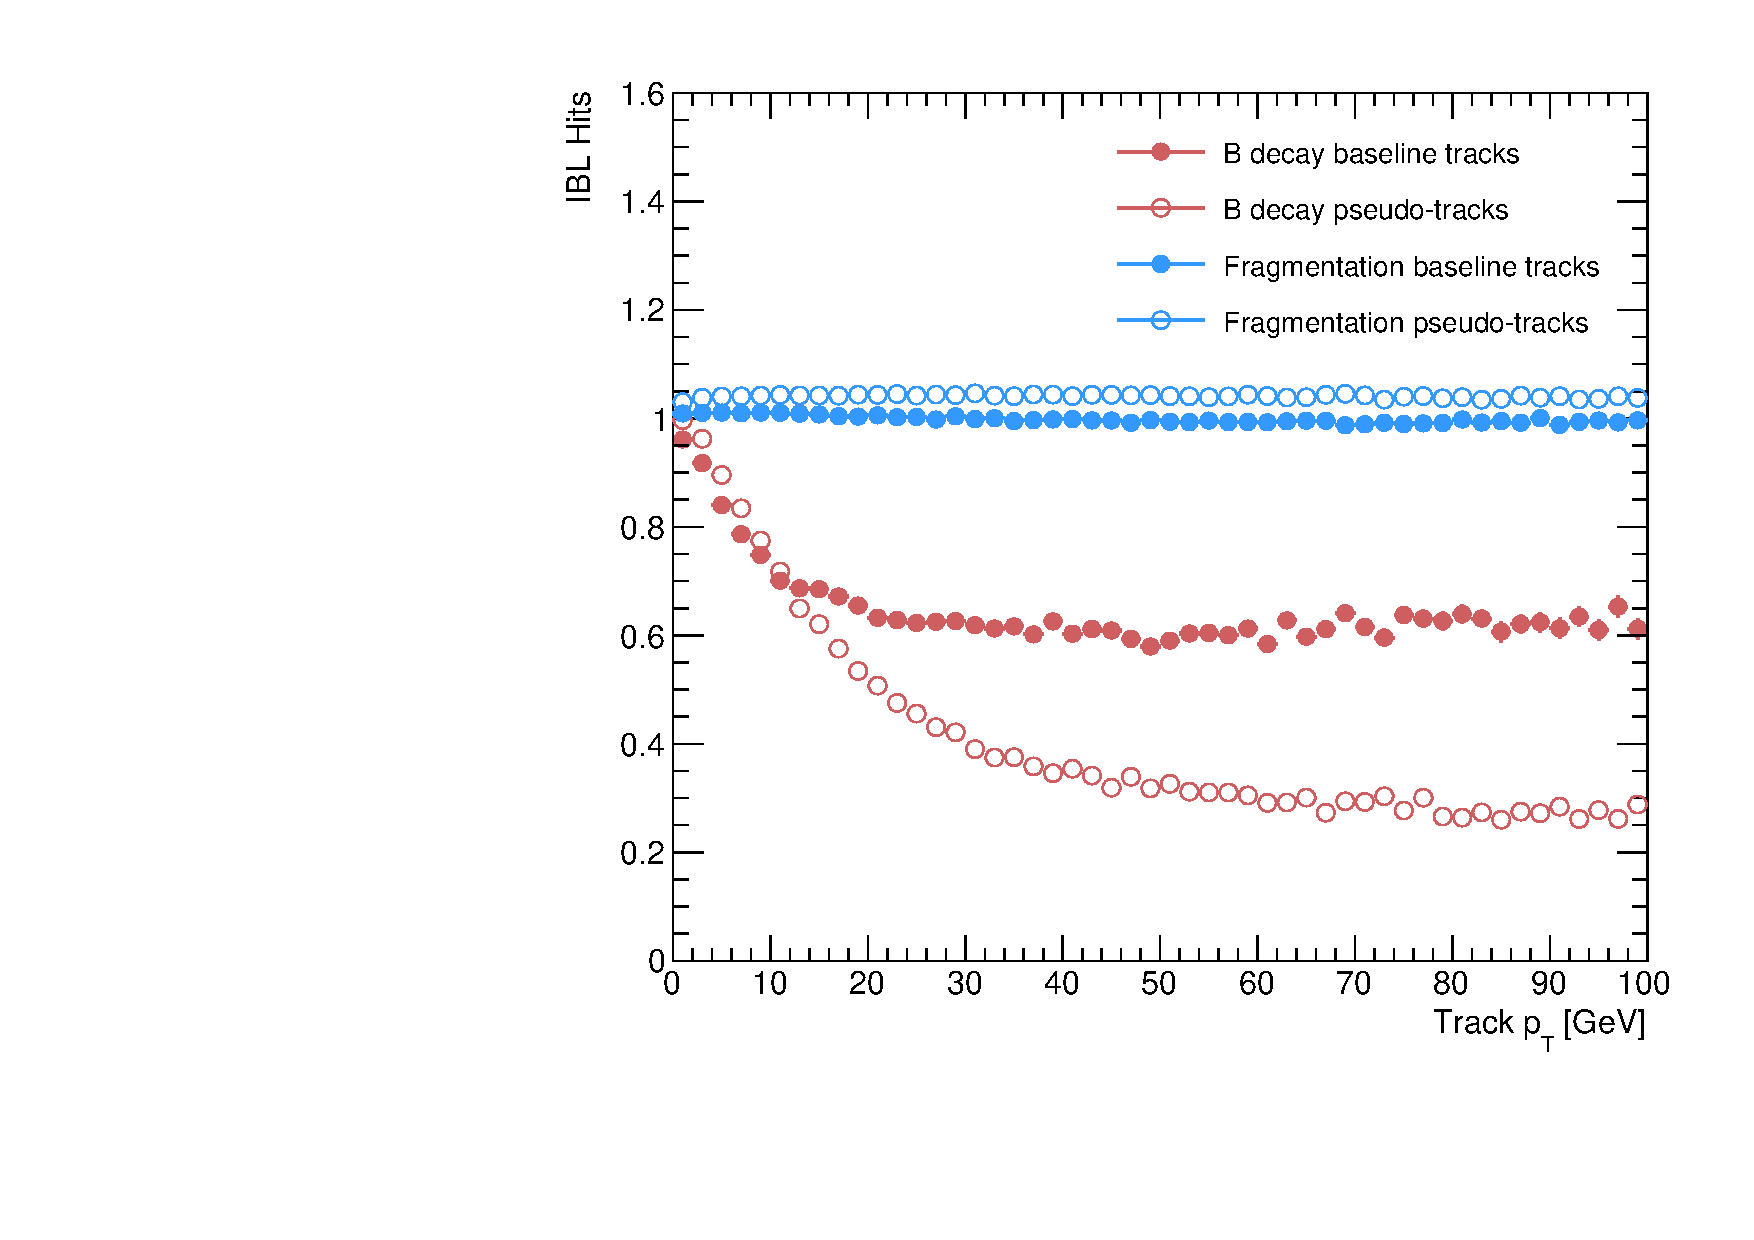
\includegraphics[width=\textwidth]{chapters/3.tracking/figs/overlay_po_nHitsOnIBL_From_B_pT.pdf}
    %\caption{}
    %\label{fig:n hits on ibl}
  \end{subfigure}%
  \begin{subfigure}{.48\textwidth}
    \centering
    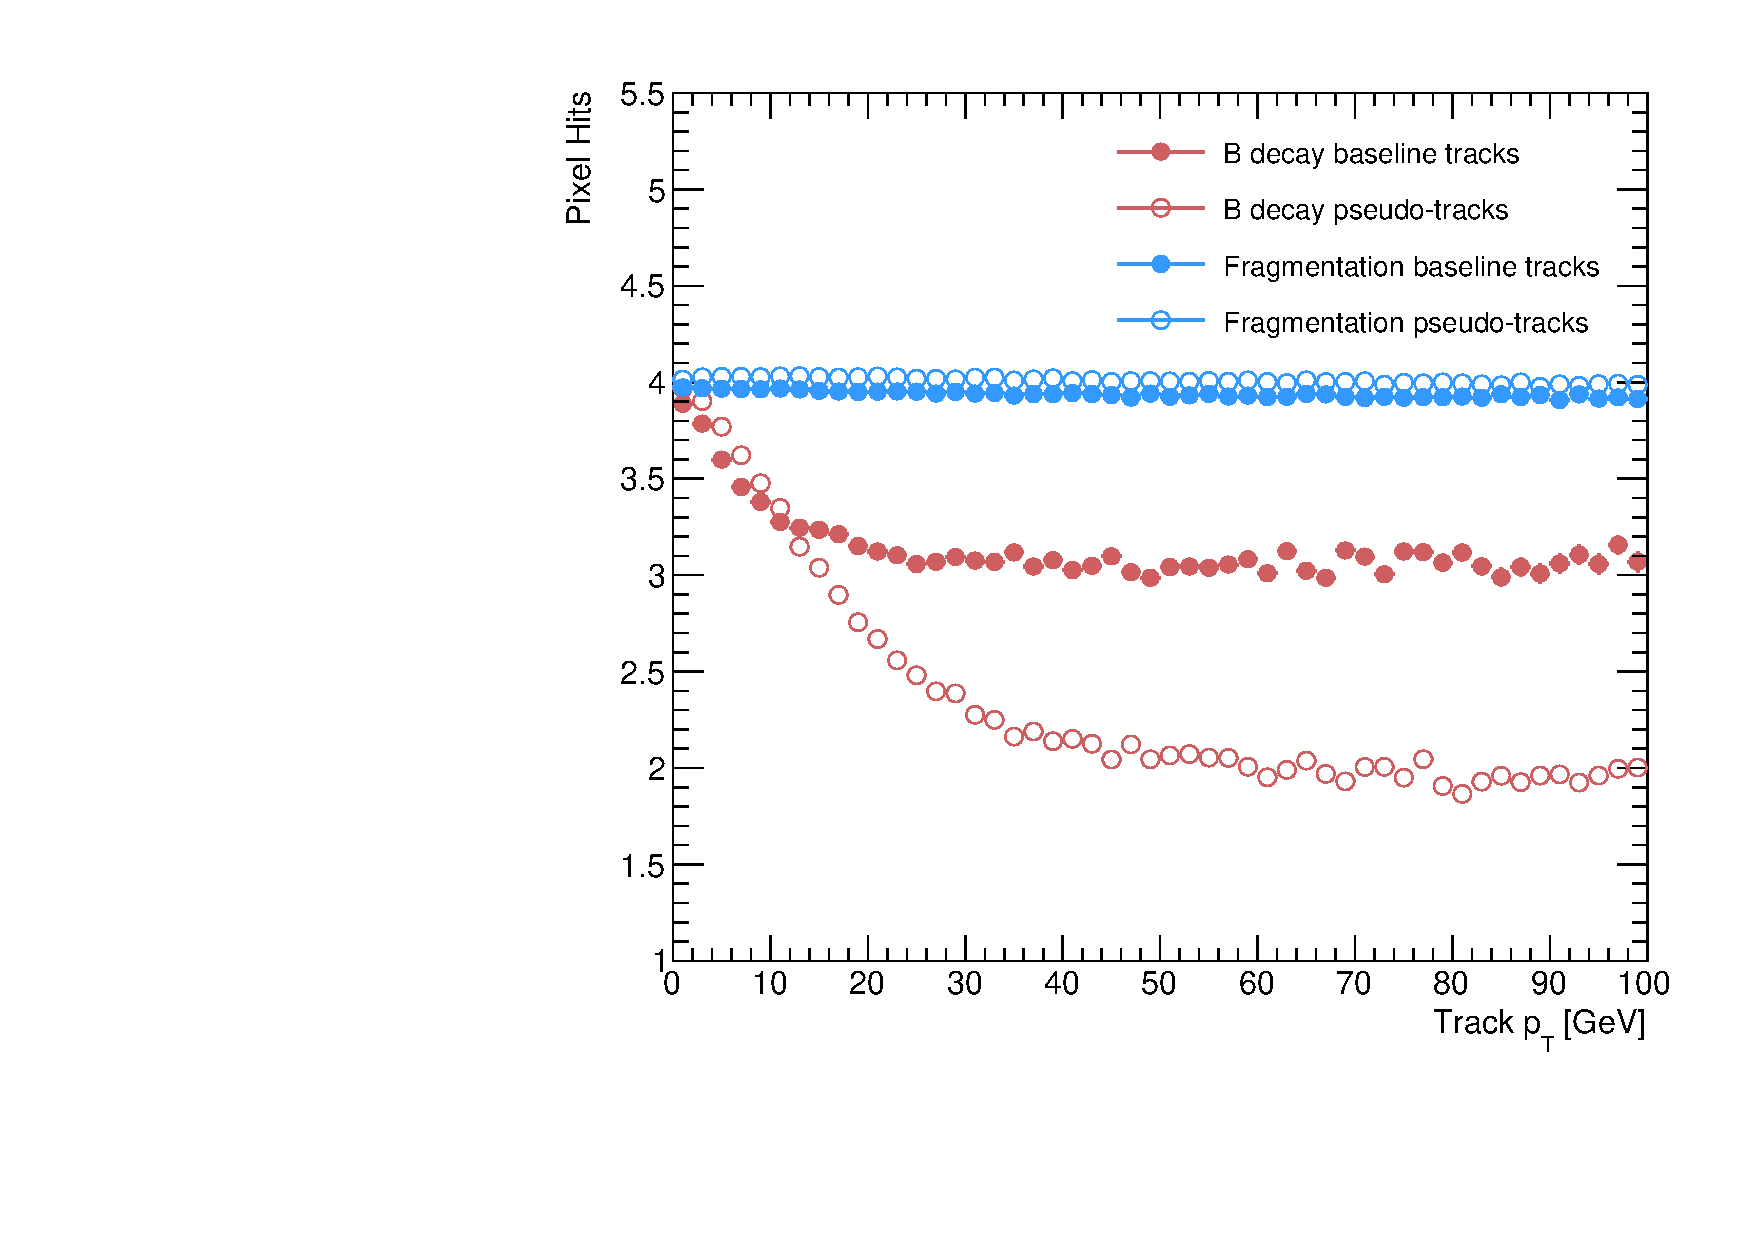
\includegraphics[width=\textwidth]{chapters/3.tracking/figs/overlay_po_nHitsOnPix_From_B_pT.pdf}
    %\caption{}
    %\label{fig:n hits on pix}
  \end{subfigure}
  \caption{
    Average hit multiplicities on the IBL (left) and the pixel layers (right) as a function of the \pT of the reconstructed track for tracks in jets in a \Zprime sample at \come{13}.
    Tracks from the weak decay of the \bhadron are shown in red, while fragmentation tracks (which are prompt) are in blue.
    Baseline tracks are those produced in the standard reconstruction described in \cref{sec:track_reco}, while pseudotracks represent the ideal performance of the ATLAS detector and are described in \cref{sec:pseudotracks}.
  }
  \label{fig:pseudo_pix_hits}
\end{figure}

These incorrect hits may skew the parameters of the track, which can in turn lower the performance of the downstream \btagging algorithms.
In particular, \btagging algorithms rely heavily on the transverse impact parameter significance \dzerosig of the track (see \cref{sec:track_parameterisation}).
The quality of this measurement is expected to be adversely affected by wrong inner-layer hits on the track.
Furthermore, multiple tracks sharing an incorrect hit can lead to the creation of spurious secondary vertices, which can cause further problems for the \btagging algorithms.

The combination of the effects described makes reconstructing tracks in the core of high \pT \bjets particularly challenging.
The reduced reconstruction efficiency of \bhadron decay tracks and incorrectly assigned hits is thought to be the primary cause of the observed drop in \btagging efficiency at high energies, however further study is required to determine which effect may dominate.



\section{High \texorpdfstring{\pT}{pT} \texorpdfstring{\bhadron}{b-hadron} Tracking Improvements}\label{sec:b_track_reco_improvements}

In \cref{sec:sharedhits} pseudotracks, a key tool for studying the ideal tracking performance of the \ATLAS detector, are used to study the shared hit requirements on tracks in the dense cores of \highpt \bjets.
Meanwhile \cref{sec:gx2f_opt} details a study which investigated modifying the global track fitter to improve reconstruction performance in this regime.
%Not detailed here is an investigation into the bcut + refit method. Shown not to be promising, as, even though an improvement in the \bhadron decay track efficiency was observed, the corresponding increase in the fake track was shown to be unacceptable.


\subsection{Shared Hits}\label{sec:sharedhits}

The ambiguity solver is not run for pseudotracks.
However, if the standard track collection is produced alongside the pseudotracks, then cluster splitting neural networks will be run for the standard tracks, and the resulting classification of clusters will be propagated to hits on pseudotracks.
This quirk allows one to study the inefficiencies of the cluster splitting process, and relatedly to determine whether shared hit cuts in the ambiguity solver are too loose or too tight.

The fraction of hits that are shared for the IBL and the B-layer is shown in \cref{fig:shared_hits_pseudo}.
The shared hits on pseudotracks represent correctly assigned hits from merged clusters that were not able to be classified as split by the cluster splitting neural networks.
As such, these represent the number of shared hits the ambiguity solver should aim to allow given the current performance of the cluster splitting algorithm.
For shared hits on the IBL for particles produced before the IBL, the baseline selection appears to be successful in disallowing excessive numbers of shared hits.
However, the ambiguity solver fails to limit shared hits for those particles produced after the IBL, reflecting the previously discussed problem of displaced tracks picking up incorrect hits.
In contrast, it is clear that for the B-layer, the ambiguity solver is being overly aggressive in its rejection of shared hits, motivating further study in this area.

\begin{figure}[!htbp]
    \centering
    \begin{subfigure}{.48\textwidth}
      \centering
      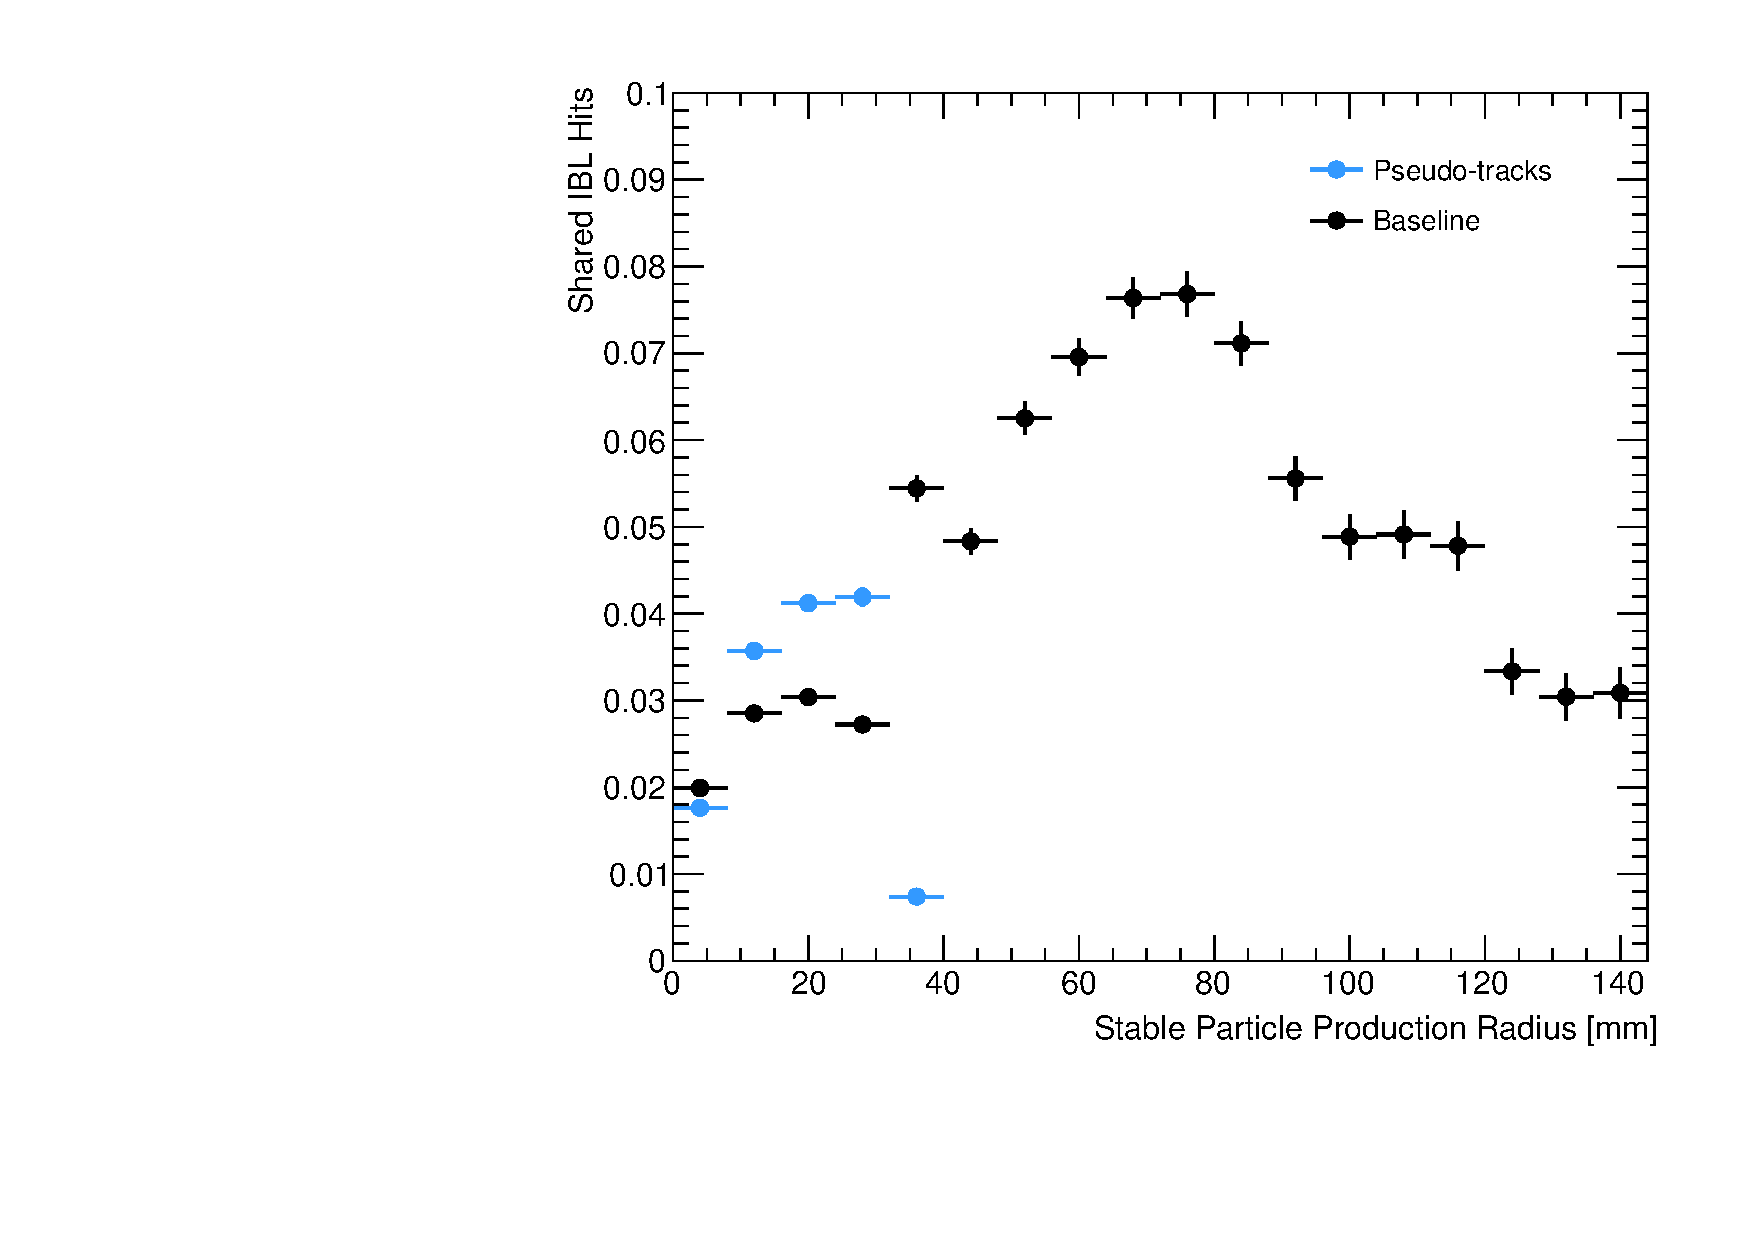
\includegraphics[width=\textwidth]{chapters/3.tracking/figs/po_nSharedOnIBL_From_B_DL.pdf}
      %\caption{}
      %\label{fig:shared_hits_pseudo on IBL}
    \end{subfigure}%
    \begin{subfigure}{.48\textwidth}
      \centering
      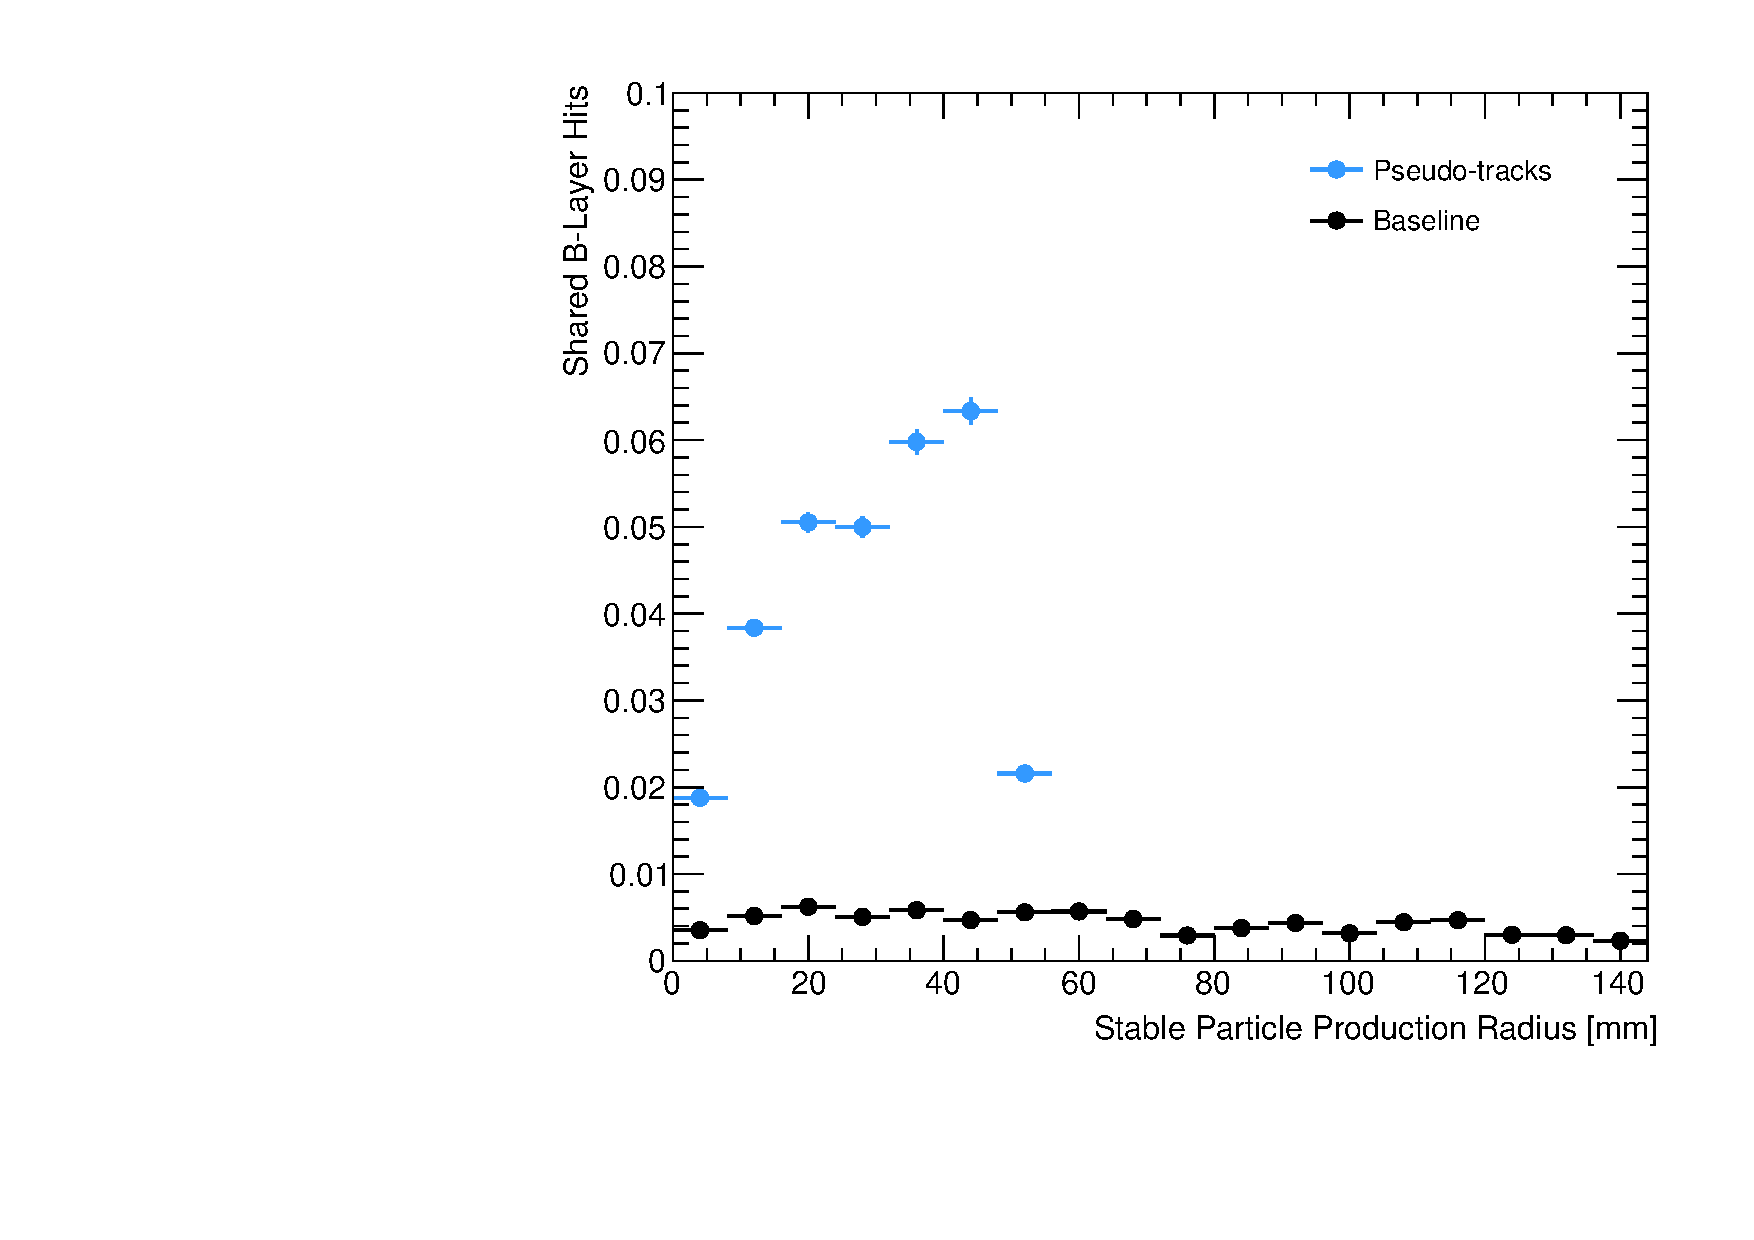
\includegraphics[width=\textwidth]{chapters/3.tracking/figs/po_nSharedOnBL_From_B_DL.pdf}
      %\caption{}
      %\label{fig:shared_hits_pseudo on B}
    \end{subfigure}
    \caption{
      The fraction of IBL (left) and B-layer (right) hits which are shared on \bhadron decay tracks as a function of the production radius of the \bhadron decay product for tracks in jets in a \Zprime sample at \come{13}. 
      Pseudotracks represent the ideal performance given the ATLAS detector, see \cref{sec:pseudotracks}.
    }
    \label{fig:shared_hits_pseudo}
\end{figure}



\begin{comment}

\subsection{Looser Track Cuts \& Track Refit Procedure}\label{sec:bcut and refit}
A solution for the problem of wrong inner-layer hits on $B$ tracks had previously been developed. This solution selects tracks which pass a $b$-jet Region of Interest (ROI) selection, and then removes the innermost hits on these tracks based on the result of a ``refit'' procedure. The refit procedure runs as follows. Each track is refitted without the innermost hit, and if there is a significant improvement in the fit quality (the $\chi^2$ of the track fit divided by the number of degrees of freedom on the track $n$), the innermost hit is rejected and the new track is replaces the old. If the fit quality does not improve by a certain amount, the initial track is kept. This procedure is recursively applied. The $b$-jet ROI selection selects tracks that are matched within $dR < 0.14$ ($|\eta| < 0.1$, $|\phi| < 0.1$) of a CaloCluster with $E_T > 150$ GeV. The track itself must also pass a transverse momentum cut with \pT$>15$ GeV. The refit procedure was previously shown to lead to a reduction in the rate of wrongly assigned IBL hits on $B$ decay tracks (see \cref{fig:refit optimisation results sub2}). However, this apparent improvement did not lead to an increase in $b$-tagging performance. It was found that the refit procedure also removed unacceptable numbers of good hits, degrading the quality of un-problematic tracks, shown in \cref{fig:refit optimisation results sub1}. This is likely the cause of the underwhelming $b$-tagging performance improvement. 

The performance of both the ROI, and the hit removal using track fit information, is examined, and an attempt at improving the performance of the refit procedure is made. Results are discussed in the following two sections.

\subsubsection{Region of Interest Optimisation}\label{sec:roi opt}

Selection cuts for the $b$-jet ROI were determined on a largely ad-hoc basis. An effort was made to systematically optimise the selection cuts. The decay tracks of \bhadrons are tightly collimated with the $B$ itself, with most decay products satisfying $dR(B, \text{track}) < 0.02$, as shown in \cref{fig:B dR match sub1}. Meanwhile, calorimeter clusters relating to the \bhadrons are generally found within $dR < 0.05$ of the $B$ \cref{fig:B dR match sub2}. In total, then, $B$ decay tracks will usually be found within $dR<0.07$ of the relevant calorimeter cluster, which suggests that the current $dR<0.14$ is loose by a factor of two. Similar analysis of cluster and track energy distributions found that the related cuts were also loose, and so they were modified from $E_T > 150$ GeV to $E_T > 300$ GeV, and from $p_T > 15$ GeV to $p_T > 30$ GeV. 

Additionally examined in the course of this work was the fake rate of the $b$-jet ROI. The distributions in \cref{fig:cluster purity in pt} demonstrate that most of clusters passing the $E_T > 150$ GeV selection were unable to be matched to a nearby \bhadron using truth information. Clusters that pass the selection but do not correspond to energy depositions from \bhadrons lead to fake ROIs. As a consequence of these distributions, tracks selected by the ROI are largely impure in the desired \bhadron tracks.

The modified ROI was used to re-run the refit procedure. A comparison of ``standard'' and ``optimised'' (using the optimised $b$-jet ROI) refit procedures is found in \cref{fig:refit optimisation results}. These results show that whilst tighter selection cuts did lead to a recovery of some good hits (\cref{fig:refit optimisation results sub1}), performance with respect to the baseline is still significantly degraded. 

%
\begin{figure}[!htbp]
    \centering
    \begin{subfigure}{.4\textwidth}
      \centering
      %\includegraphics[width=\textwidth]{res/figs/results/tracking/Bhad-track-dR-3.png}
      \caption{}
      \label{fig:B dR match sub1}
    \end{subfigure}%
    \begin{subfigure}{.4\textwidth}
      \centering
      %\includegraphics[width=\textwidth]{res/figs/results/tracking/Bhad-CC-dR-3.png}
      \caption{}
      \label{fig:B dR match sub2}
    \end{subfigure}
    \caption{Distributions of angular distance $dR$ between \bhadrons and their weak decays and other fragmentation tracks (\cref{fig:B dR match sub1}), and the distribution of angular distance $dR$ between \bhadrons and the calorimeter clusters in the hadronic calorimeter (\cref{fig:B dR match sub2}). In \cref{fig:B dR match sub1}, the tracks from the weak decay of the $B$ are significantly more collimated to the $B$ than the other fragmentation tracks.}
    \label{fig:B dR match}
\end{figure}
%

\subsubsection{Fit Quality as a Discriminant for Wrong Hits}
As mentioned, tracks selected by the ROI are refitted without their innermost hit, and, if an improvement in fit quality is observed, the hit is rejected. In order to test the effectiveness of this procedure, a dataset of two sets of tracks was produced. The first set contained unmodified baseline-reconstructed tracks. The second contained the same tracks as the first, but modifications made during reconstruction removed the innermost hit on each track. Then, using Monte Carlo (MC) truth information, a track-by-track fit quality comparison was made for tracks with good and wrong innermost hits. 

It is clear from the distributions in \cref{fig:refit chi2 dists} that the fit quality improvement (measured by fractional change in $\chi^2/n$ of the track before and after the innermost hit is removed) is not a discriminating variable for wrong hits, and indeed attempted optimisations of the of the refit procedure based on these distributions were found to be ineffectual. While wrong hits are likely to degrade the track fit, it is also true that any additional measurement, good or wrong, constrains the track, and therefore removal of that measurement will be likely to lead to an increase in the $\chi^2/n$ of the track. Removing hits in this way is therefore problematic.
%
\begin{figure}[!htbp]
    \centering
    \begin{subfigure}{.4\textwidth}
      \centering
      %\includegraphics[width=\textwidth]{res/figs/results/tracking/ROI-purity.png}
      \caption{}
      \label{fig:cluster purity in pt}
    \end{subfigure}%
    \begin{subfigure}{.4\textwidth}
      \centering
      %\includegraphics[width=\textwidth]{res/figs/results/tracking/hitdrop-chi2.png}
      \caption{}
      \label{fig:refit chi2 dists}
    \end{subfigure}
    \caption{The distribution of cluster transverse momentum, in \cref{fig:cluster purity in pt} for both clusters that were able (orange) and unable (blue) to be matched to a \bhadron using MC truth information. The normalisation shows that the majority of clusters are not matched to \bhadrons, resulting in fake ROIs. In \cref{fig:refit chi2 dists}, the fractional improvement in track fit quality ($\chi^2/n$) is shown for all track (blue), tracks with good IBL hits (green), and tracks with wrong IBL hits (orange). The distributions are overlapping, suggesting that the $\chi^2/n$ improvement is not a good discriminator of good and wrong hits.}
    \label{fig:cluster chi2 info}
\end{figure}
%

\subsubsection{Conclusion}
The work outlined in the two preceding sections has uncovered issues with both the $b$-jet ROI, and the methodology of identification and removal of wrong hits on tracks inside a given ROI. Attempts were made to optimise the selection cuts of the ROI, however the large background of energetic phenomena produced in collisions that are not \bhadron related means that the ROI is largely unsuccessful in selecting a pure sample of likely \bhadron candidates. An additional effort was made to improve the removal of wrong hits using other information in addition to the track fit improvement. Information such as the type and locations of its, and track $d_0$ were considered. While progress here was not insignificant, without substantial overhaul of the ROI to improve $B$ purity, the results were not strong enough to demonstrate any viable solutions that would successful target and then improve \bhadron decay tracks.
%
\begin{figure}[!htbp]
    \centering
    \begin{subfigure}{.4\textwidth}
      \centering
      %\includegraphics[width=\textwidth]{res/figs/results/tracking/po_nGoodHitsOnIBL_From_B_DL.pdf}
      \caption{}
      \label{fig:refit optimisation results sub1}
    \end{subfigure}%
    \begin{subfigure}{.4\textwidth}
      \centering
      %\includegraphics[width=\textwidth]{res/figs/results/tracking/po_nWrongHitsOnIBL_From_B_DL.pdf}
      \caption{}
      \label{fig:refit optimisation results sub2}
    \end{subfigure}
    \caption{Distributions of good (\cref{fig:refit optimisation results sub1}) and wrong (fig:refit optimisation results sub2) hit assignment rates on the IBL for tracks using baseline tracking (black), the original unmodified refit procedure (green), and the refit procedure with an optimise set of ROI selection cuts (blue). The IBL lies at a radius of 33 mm from the beam pipe. Hence, particles produced with a production radius greater than this cannot leave good hits on the IBL.}
    \label{fig:refit optimisation results}
\end{figure}
%
Alongside the refit procedure, a ``Bcut'' cut scheme was suggested in order to improve reconstruction performance. This consisted primarily of loosening the shared hit cuts in the ambiguity solver. While this did lead to a measurement increase in track reconstruction efficiency (see \cref{fig:b_track_eff}), it was determined that the corresponding increase in fake tracks (i.e. those tracks for which the majority of hits do not come from a single truth particle) was too large to justify the implementation of the ``Bcut'' scheme. In conclusion, then, a different approach is required to address the problems discussed.

\end{comment}


\subsection{Global \texorpdfstring{$\chi^2$}{chi2} Fitter Outlier Removal}\label{sec:gx2f_opt}

As part of the track fit an outlier removal procedure is run in which suspicious hits are identified and removed.
This section documents ongoing studies into improving hit-to-track assignment by using the Global $\chi^2$ Fitter (GX2F) to identify and prevent incorrect hits from being assigned to tracks during the track fit.
This is in contrast to a previously investigated approach \cite{AdorniBraccesiChiassi:2021irw} which attempted to identify and remove incorrect hits after the reconstruction of the track.

The GX2F code, as a relatively low-level component of track reconstruction, has not undergone significant modification for several years, and was originally only optimised in the context of prompt, isolated tracks.
Since then, a new tracking sub-detector, the IBL, was installed.
The motivation for looking at the GX2F is that this change may require the re-optimisation of the GX2F code, and in particular the outlier removal procedure.
Further motivation for this approach comes from the low rate of labelled outliers in baseline tracking, in contrast to the relatively higher rate of tracks with an incorrect IBL hit.
%For example, while approximately 15\% of \bhadron decay tracks have a wrong IBL hit (a value which only increases with the \pT of the \bhadron), less than 1\% of this tracks have had their IBL hit labelled and removed as an outlier.


\subsubsection{Implementation}
The outlier removal procedure for the pixel detector is described in this section. The hits on the track are looped over in order of increasing radial distance to the beam pipe. For each hit, errors $\sigma(m_i)$ on the measurement of the transverse and longitudinal coordinates are calculated. These errors are dependent on the sub-detector which recorded the measurement (some sub-detectors are more precise than others). Additionally, a residual displacement $r_i = m_i - x_i$ between the predicted position of the track $x_i$ (inclusive of the current measurement), and the position of the hit itself, $m_i$, is calculated. The pull $p_i$ on the track state due to the current measurement is calculated according to
%
\begin{equation}
    p_i = \frac{m_i - x_i}{\sqrt{\sigma(m_i)^2 - \sigma(x_i)^2}}
\end{equation}
%
This pull is computed for the transverse and longitudinal coordinates of the measurement, and the maximum of the two is selected and checked to see if it exceeds a certain selection threshold. If it does, the hit will be removed if the track also exceeds a threshold on the total $\chi^2/n$, where $n$ is the number of degrees of freedom on the track.
The results of varying the outlier selection and $\chi^2/n$ thresholds are described below.


\subsubsection{Selection Optimisation}

A systematic variation of the outlier selection and $\chi^2/n$ thresholds has been carried out.
Both thresholds were reduced in fixed step sizes of 0.25 for the outlier selection threshold and 1 for the $\chi^2/n$ threshold.
The value of the outlier selection threshold was reduced from 4 down to 1.75, a change which affects the silicon layers (the TRT has separate outlier removal logic).
Furthermore, a specific cut for the IBL was introduced, and after optimisation is set to 1.25.
The second threshold on the track $\chi^2/n$ was also reduced from 7 to 4.
Finally, instead of taking the maximum of the pulls in the longitudinal and transverse directions, a quadrature sum is taken of these two values and used.
This variation is labelled ``Mod GX2F'' and was found to improve performance.
The results for the best performing selections are discussed below.

The results shown in \cref{fig:gx2f_opt_hits} demonstrate a reduction in wrong hit assignment whilst also improving slightly the rate at which good hits are assigned to tracks.
For a \SI{1}{\TeV} \bhadron, the rate to assign good hits to the corresponding decay tracks increases by approximately \pct{10}, while the rate to assign incorrect hits decreases by approximately \pct{16}.
The improvements are also observed when looking inclusively in all tracks, which avoids the need for a specific \bjet region-of-interest selection.

\begin{figure}[!htbp]
    \centering
    \begin{subfigure}{.48\textwidth}
      \centering
      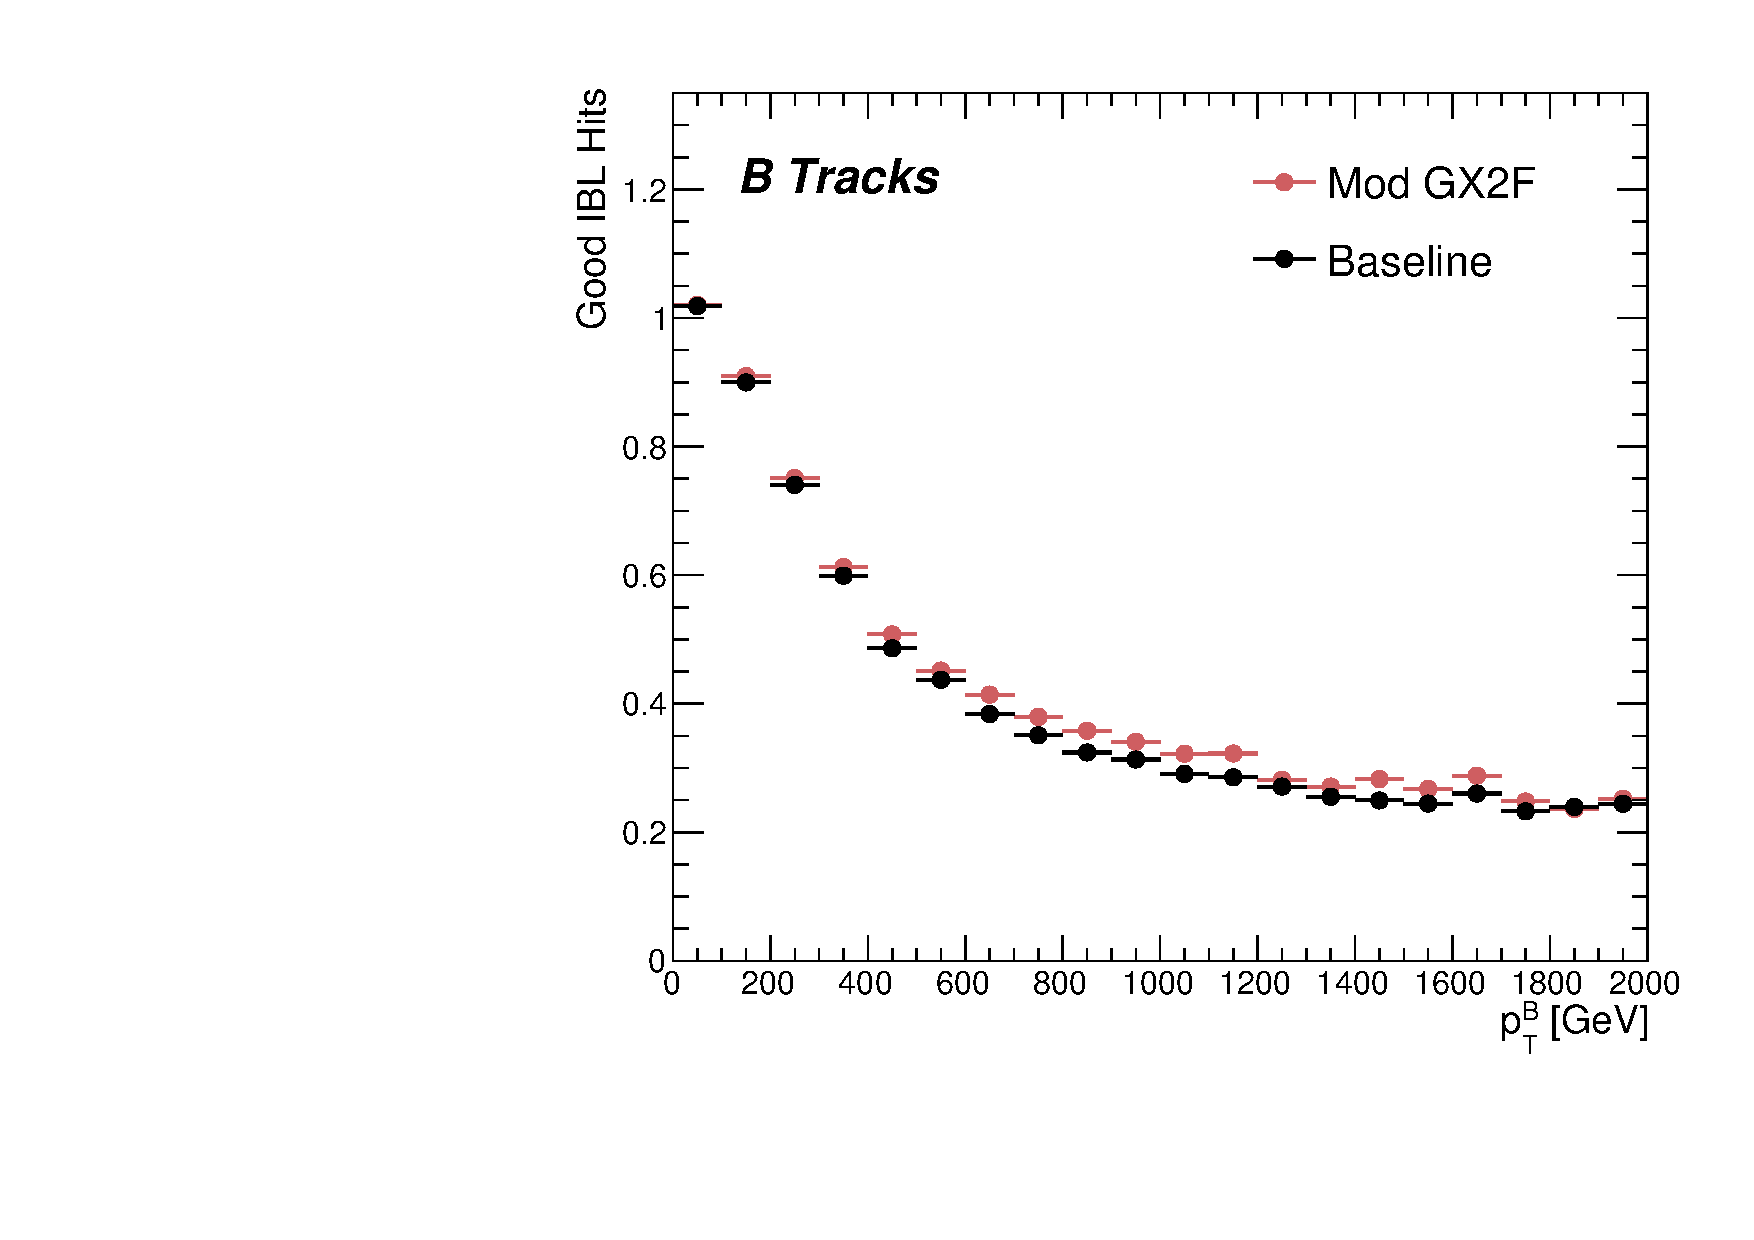
\includegraphics[width=\textwidth]{chapters/3.tracking/figs/p_nGoodHitsIBL_pTB_From_B.pdf}
    \end{subfigure}%
    \begin{subfigure}{.48\textwidth}
      \centering
      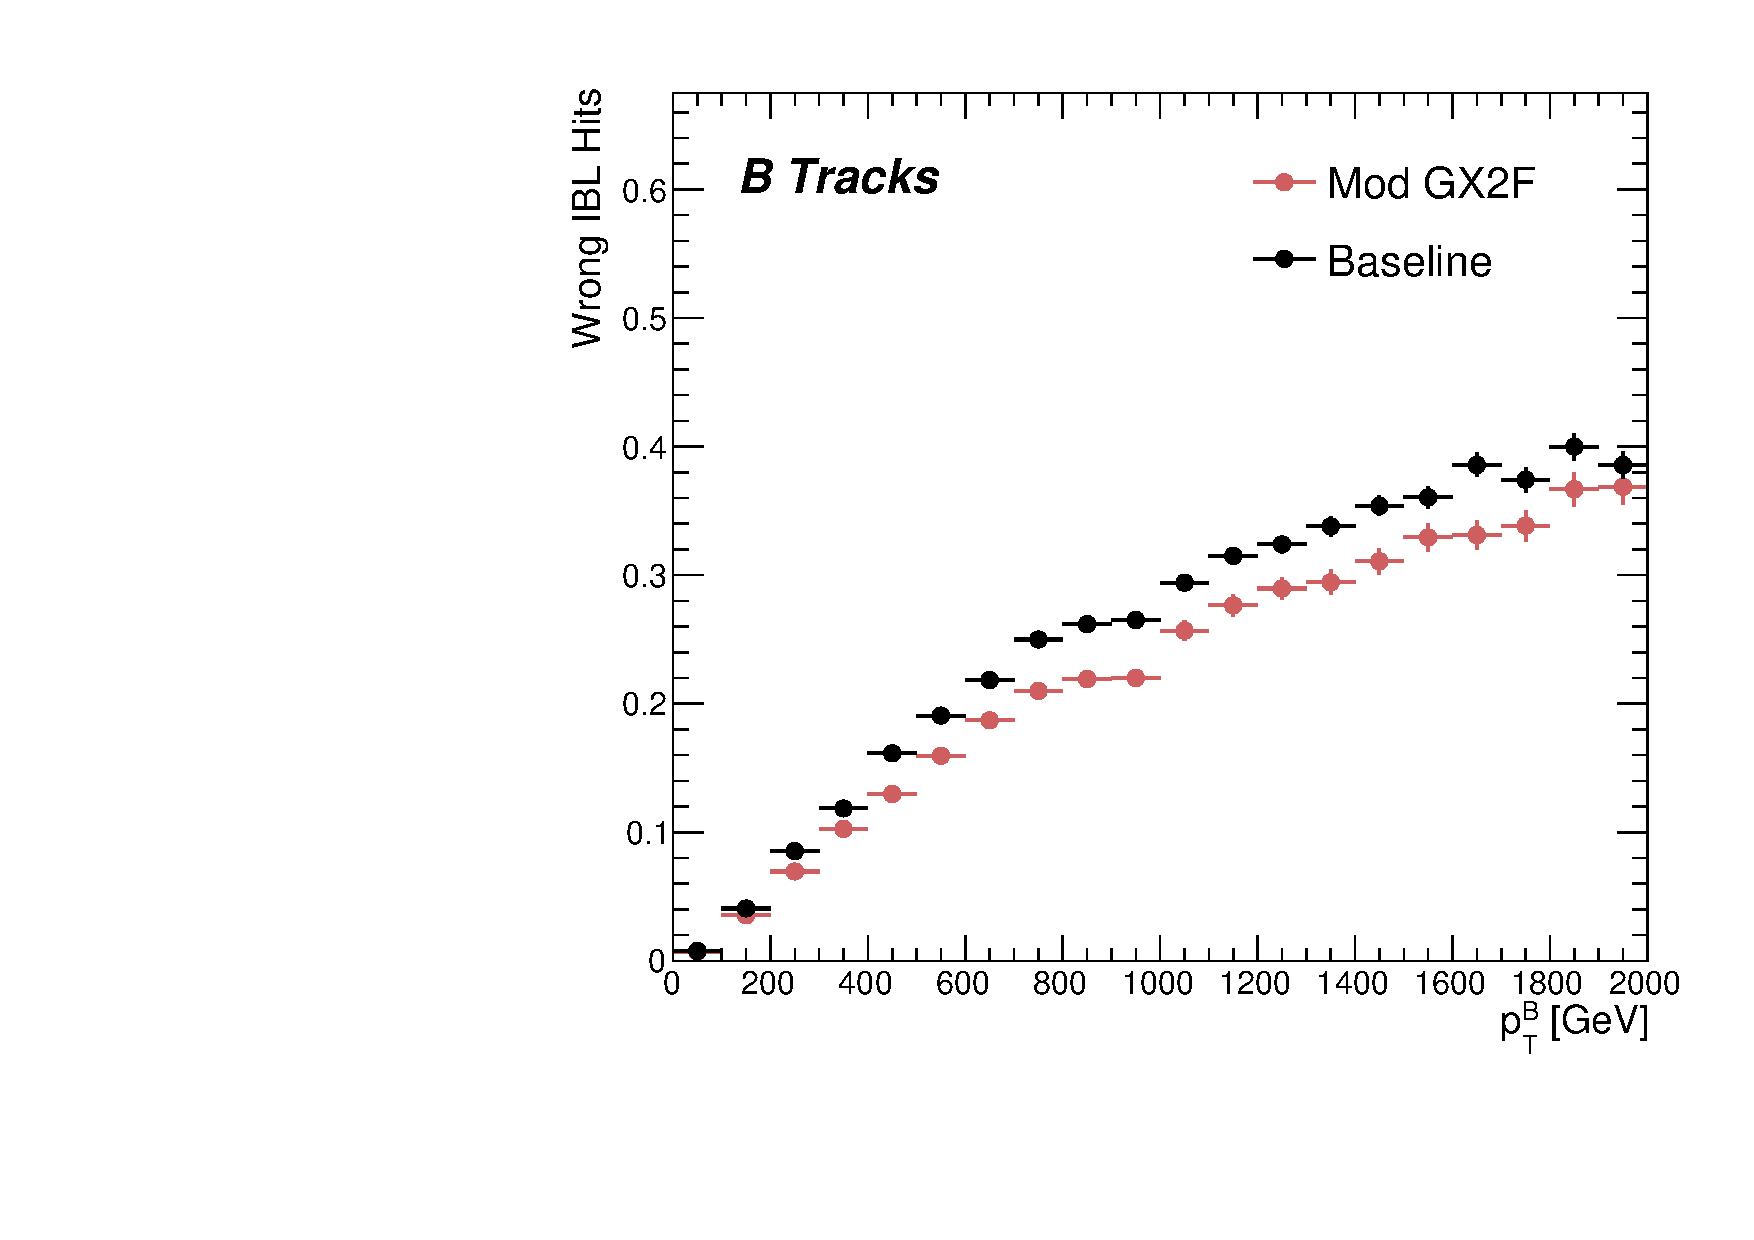
\includegraphics[width=\textwidth]{chapters/3.tracking/figs/p_nWrongHitsIBL_pTB_From_B.pdf}
    \end{subfigure}
    \caption{
      The average number of good (left) and wrong (right) IBL hits as a function of \bhadron \pt for tracks in the \Zprime sample.
      The baseline tracking performance (black) and the modified version of the outlier removal procedure (red) are shown.
    }
    \label{fig:gx2f_opt_hits}
\end{figure}

Additionally, a modest improvement of all track parameter resolutions and pulls is observed.
The improvement for the transverse impact parameter pull is shown in \cref{fig:gx2f_opt_pulls}.
Note also that the large pulls for \highpt tracks indicates that the uncertainties are not well modelled.
The results demonstrate an improvement in hit assignment, unchanged reconstruction efficiency, and modest improvement in track parameter resolutions and pulls.
In addition, the inclsuive truth-matching probability of tracks is unchanged (see \cref{sec:track_labelling}), suggesting that there is no significant increase in fake track rates. The changes are expected to have a negligible impact on computational resources.

\begin{figure}[!htbp]
    \centering
    \begin{subfigure}{.48\textwidth}
      \centering
      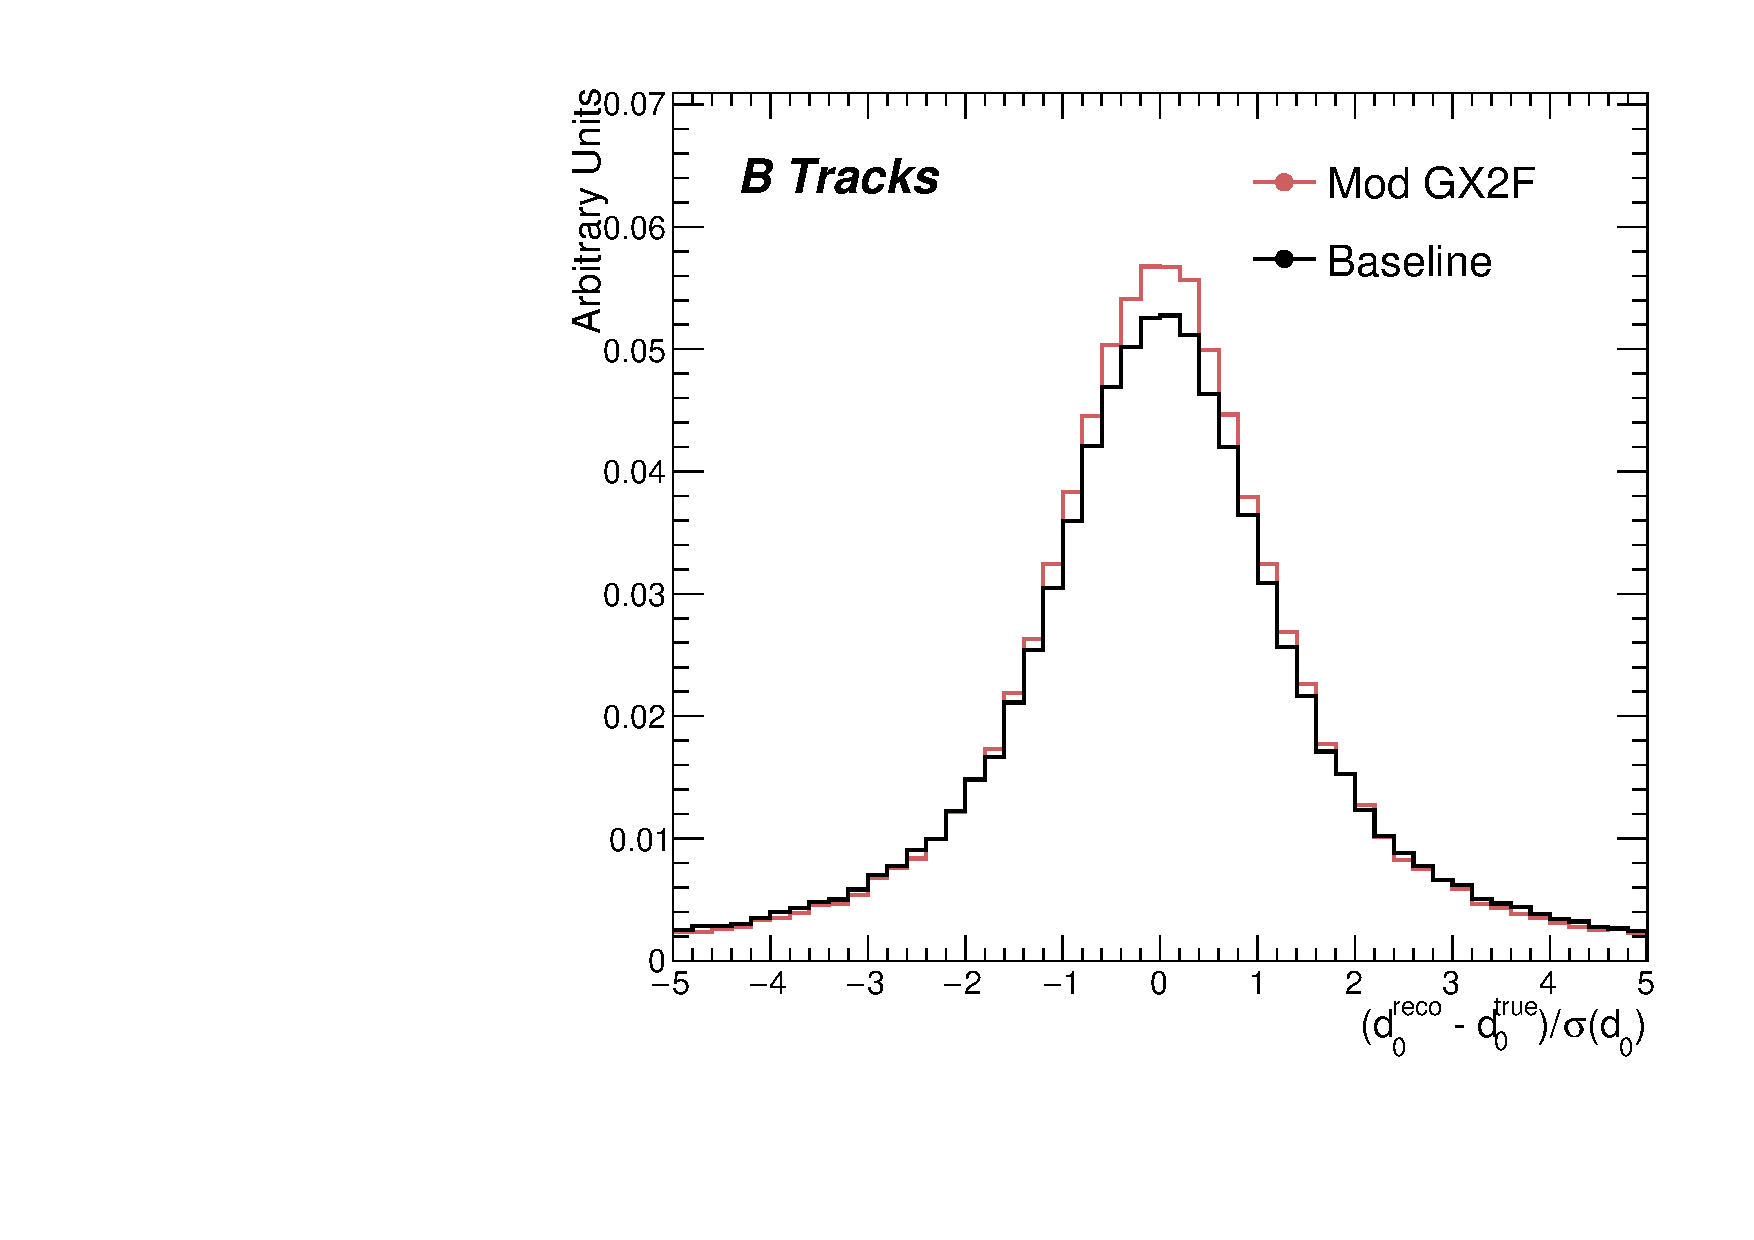
\includegraphics[width=\textwidth]{chapters/3.tracking/figs/h_recoTruthPull_d0_From_B.pdf}
      %\caption{}
      %\label{fig:d0 pull}
    \end{subfigure}%
    \begin{subfigure}{.48\textwidth}
      \centering
      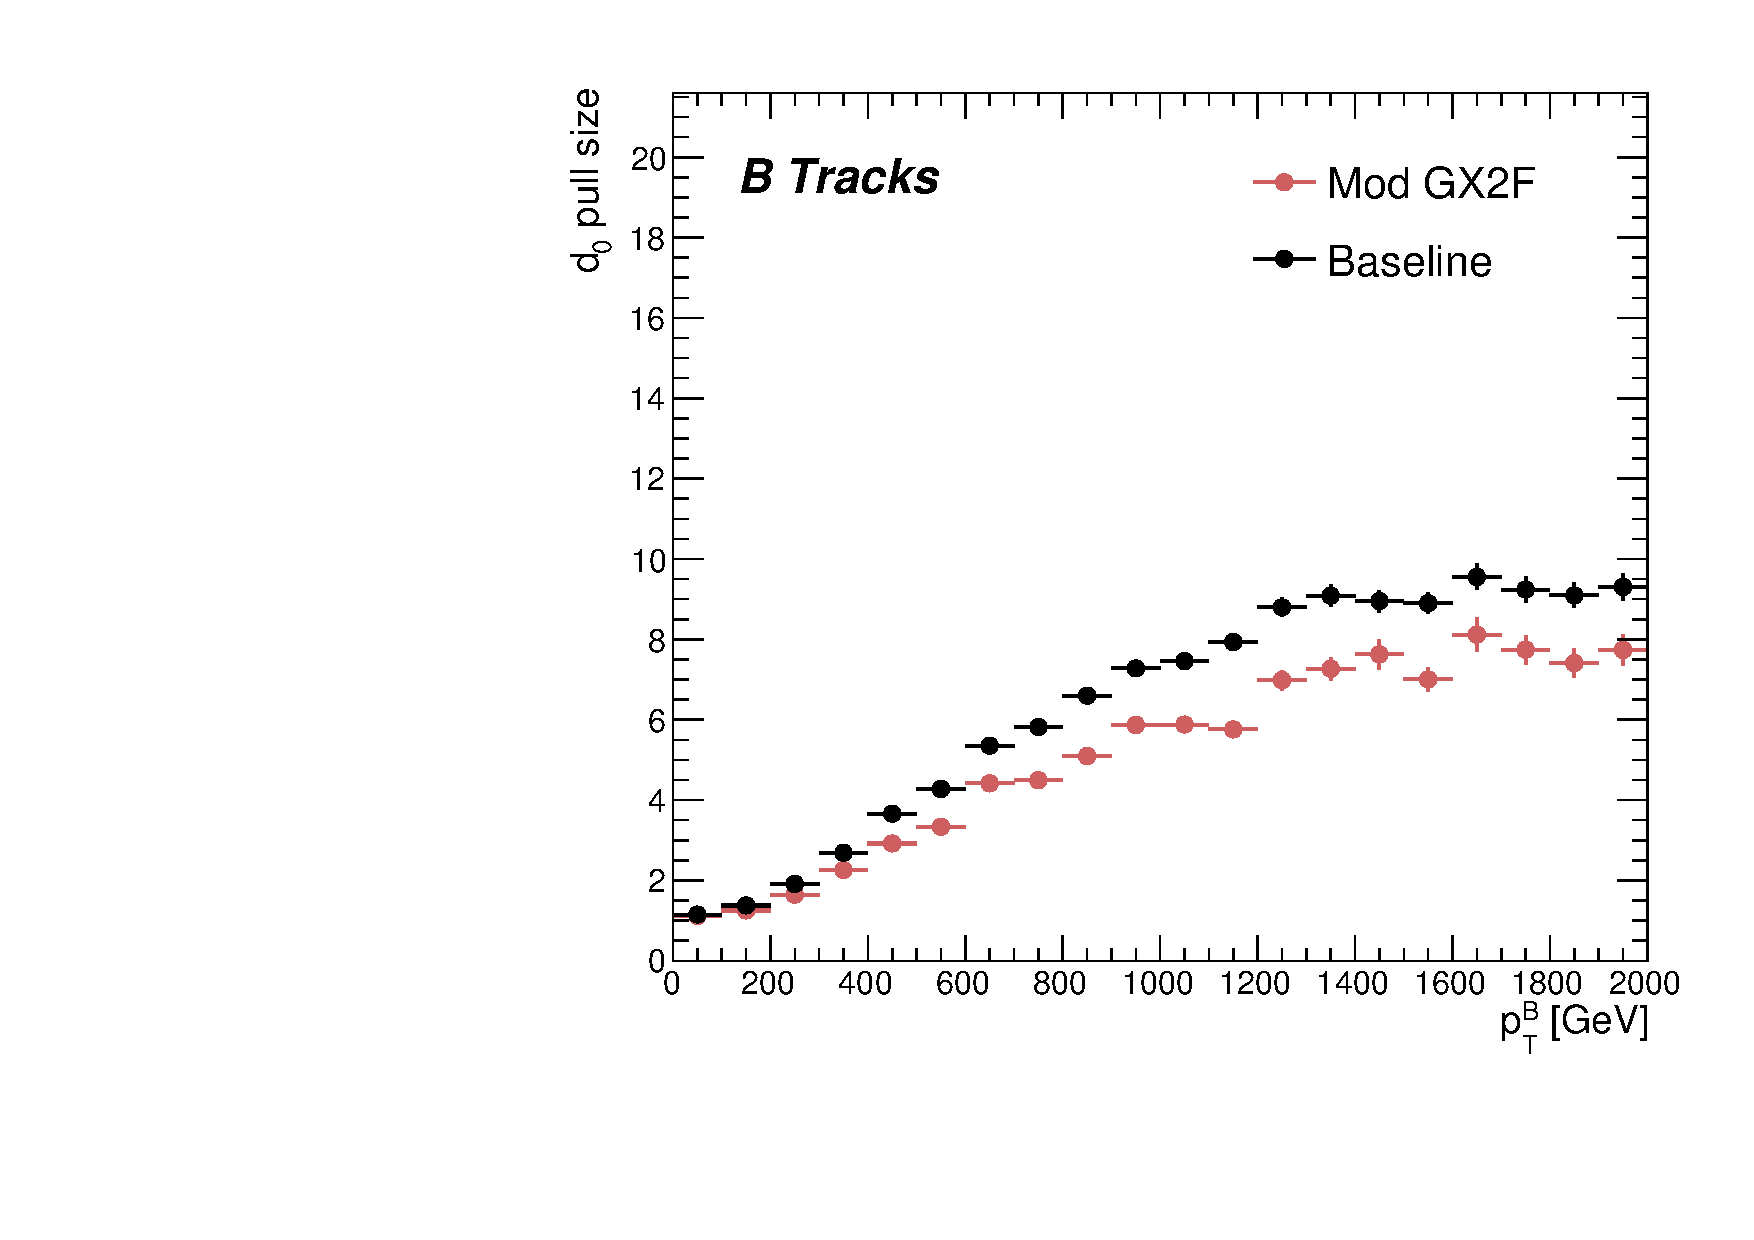
\includegraphics[width=\textwidth]{chapters/3.tracking/figs/p_d0_pull_size_pTB_From_B.pdf}
      %\caption{}
      %\label{fig:z0 pull}
    \end{subfigure}
    \caption{
      (left) \bhadron decay track \dzero pulls (\dzero/\dzerosig) for baseline and modified GX2F tracks in the \Zprime sample. 
      (right) The absolute value of the \dzero pull as a function of the truth \bhadron transverse momentum.
    }
    \label{fig:gx2f_opt_pulls}
\end{figure}




\section{Conclusion}\label{sec:trk_btag_conclusion}

In this section, the difficulties facing efficient and accurate  track reconstruction, and hence performant \btagging, have been outlined.
The ambiguity solver, which attempts to clean or reject tracks which have an excess of shared hits, is shown to be overly aggressive in the rejection of \bhadron decay product track candidates.
The ambiguity solving process relies on a complicated pre-defined selection which has not been optimised for high transverse momentum \bhadron track reconstruction.
These conclusions have motivated further ongoing studies into the improvement of the track reconstruction in dense environments and the \highpt regime, such as those in \rcite{2022DonalTrackReco}.

An optimisation of the outlier removal process in the global $\chi^2$ fitter was carried out.
The results of the optimisation show that more aggressive removal of outlier hits can lead to fewer wrong hits being assigned to tracks, and improvements in the pulls of the track parameters.


\subsubsection{Future Work}
The studies were carried out in \rtwoone of the \ATLAS software, and need to be reproduced using the newer \rtwotwo to confirm the results against other changes in the baseline tracking configuration.
It is also necessary to study the impact of the improved outlier removal on the downstream \btagging algorithms.
Thanks to the all-in-one flavour tagging approach described in \cref{chap:gnn_tagger}, this will in future be easier to study.

As there are some known data-MC discrepancies, fine tuned optimisation such as the work presented here presents an opportunity to over-optimise the tracking algorithms on MC.
As such, further studies validating the improved outlier removal procedure on data are required.

  \chapter{Track Classification NN}\label{chap:track_classification_mva}

This chapter details work on implementing a neural network (NN) to predict the truth origin of reconstructed tracks.
An introduction to the formalism of machine learning is given in \cref{sec:ml_background}.
In \cref{sec:track_labelling}, the truth origin label is defined, and in \cref{sec:fake_track_mva} these labels are used to train a machine learning model that can effectively discriminate between good and fake tracks.
Several studies motivated this work by demonstrating that at high \pt, the performance of the low-level \btagging algorithms was degraded by the presence of large numbers of poorly reconstructed or fake tracks.
If a separate algorithm could be trained to detect fake tracks, these could be removed before their input to the \btagging algorithms with the aim of improving performance.
The identification of fake tracks could also be used to improve the reconstruction of other physics objects which rely on tracking information, for example $\tau$ leptons or track-jets.


\section{Machine Learning Background}\label{sec:ml_background}

Over the past few decades, machine learning (ML) techniques have become increasingly prevalent in High Energy Physics experiments due the increased volumes of high-dimensional data and improvements in the field of deep learning.
Machine learning is the process by which a computer program uses data to infer suitable parameters for a predictive model.
This is opposed to providing explicit instructions on how to perform a task.
A subfield known as \textit{supervised learning} is used in this work, and consists of exposing a model to a large number of labelled examples in order to extract relationships between the input data and their labels.
These relationships are often complex, and explicitly programmed rules can fail to fully capture the relationships between inputs and outputs.

%The field of machine learning aims to design computer programs which, rather than being programmed explicitly with instructions on how to perform a specific task, instead learn from a set of labelled training examples $S_i$ how to perform the task for themselves, essentially replacing the need to manually design a program to perform a specific task.
%In this section a subset of machine learning techniques called supervised learning is described.

In the simplest case, a set of $m$ labelled training examples $S = \{ (x_1, y_1) , \ldots , (x_m, y_m) \}$ is collected.
Each element $(x_i, y_i)$ consists of a input vector $x_i  \in \mathbb{R}^{\textnormal{input}}$, and the corresponding label $y_i$.
In classification problems, these labels are integer \textit{class labels} $y_i \in \{0,\ldots,N-1\}$, where $N$ is the number of classes, which specify which of a pre-determined set of categorical classes the training example belongs to.
The rest of the discussion in this chapter is limited to binary classification problems ($N = 2$).
The two classes are often referred to as signal ($y_i = 1$) and background ($y_i = 0$), which need to be separated.
Collecting sufficient and suitable data is one of the primary challenges of machine learning, as such data is not always readily available.
Fortunately, sophisticated tools to simulate particle collisions have already been developed by the scientific community \cite{Boos:2001cv,leshouchesstandardisation}.
These tools play a key role in generating a suitably large amount of labelled data which is used to train algorithms.
More detail on the input datasets can be found in \cref{sec:track_classifier_datasets}.

After obtaining suitable training data, the next step is to define a model.
Given an input domain $\mathbb{R}^{\textnormal{input}}$ and an output domain $(0, 1)$, the model
$f_\theta: \mathbb{R}^{\textnormal{input}} \to (0, 1)$ is a parameterised functional mapping from input space to output space.
Given an input example $x_i$ and a set of parameters $\theta$, the model outputs a prediction $\hat{y}_i \in (0, 1)$ for the true label $y_i$, as in
%
\begin{equation}
    f_\theta(x_i) = \hat{y}_i .
\end{equation}
%
The output $\hat{y}_i$ is in the interval $(0, 1)$ so as to be interpreted as the probability that the input example $x_i$ belongs to the signal class.
The parameters $\theta$ of the model are randomly initialised, and the model is designed to be expressive enough to correctly map the inputs $x_i$ to the outputs $y_i$ given a reasonable optimisation of the parameters.
To perform this optimisation, the model is then trained, which amounts to showing the model a series of labelled training examples and modifying the parameters of the model based on its ability to correctly predict the labels.


\subsection{Neural Networks}\label{sec:neural_nets}

Neural networks (NNs) are a common choice for the machine learning model $f$ since they have the ability to approximate any function \cite{HORNIK1989359} and are easy to train via backpropagation \cite{rumelhart1986learning}.

\subsubsection{Artificial Neurons}

The basic functional component of a NN is the \textit{artificial neuron} or node, which is loosely inspired by a mathematical model of a biological neuron \cite{mcculloch1943logical, hopfield1987neural}.
A diagram of an artificial neuron is shown in \cref{fig:neuron}
Each neuron is defined by its parameters or \textit{weights} $\theta$ and a choice of activation function.
Each neuron takes a fixed number of inputs and computes the dot product of the input and weight vectors $x^T \theta$ and additionally adds a constant bias term $\theta_0$.
This term plays the role of a trainable constant value that is independent of the inputs.

\begin{figure}[!htbp]
    \centering
    \usetikzlibrary{matrix,chains,positioning,decorations.pathreplacing,arrows}
\begin{tikzpicture}[
    init/.style={
      draw,
      circle,
      inner sep=2pt,
      font=\Huge,
      join = by -latex
    },
    squa/.style={
      draw,
      inner sep=2pt,
      font=\Large,
      join = by -latex
    },
    start chain=2,node distance=13mm
    ]
    \node[on chain=2] 
      (x2) {$x_i^2$};
    \node[on chain=2,init] (sigma) 
      {$\displaystyle\Sigma$};
    \node[on chain=2,squa,label=above:{\parbox{2cm}{\centering Activation \\ function}}]   
      {$f$};
    \node[on chain=2,label=above:Output,join=by -latex] 
      {$\hat{y}$};
    \begin{scope}[start chain=1]
    \node[on chain=1] at (0,1.5cm) 
      (x1) {$x_i^1$};
    \end{scope}
    \begin{scope}[start chain=3]
    \node[on chain=3] at (0,-1.5cm) 
      (x3) {$x_i^3$};
    \end{scope}
    \node[label=above:\parbox{1.5cm}{\centering Bias \\ $\theta_0$}] at (sigma|-x1) (b) {};

    \draw[-latex] (x1) -- (sigma) node[midway,above] {$\theta_1$};
    \draw[-latex] (x2) -- (sigma) node[midway,above] {$\theta_2$};
    \draw[-latex] (x3) -- (sigma) node[midway,above] {$\theta_3$};
    \draw[o-latex] (b) -- (sigma);

    \draw[decorate,decoration={brace,mirror}] (x1.north west) -- node[left=10pt] {Inputs} (x3.south west);
\end{tikzpicture}
    \caption{
      A diagram displaying the logical flow of a single neuron with three inputs $x_i^j$.
      Each input is multiplied by a weight $\theta_j$, and the resulting values are summed.
      A bias term $\theta_0$ is added, and the result $z$ is passed to an activation function.
      Each neuron can be thought of as a logistic regression model.
    }
    \label{fig:neuron}
\end{figure}

The output $z$ of the dot product and bias term is fed into an activation function $g(z)$.
The activation function has several uses, most notably acting as a source of non-linearity and bounding the output of the neuron.
Some common activation functions (sigmoid, tanh, ReLU and SiLU) \cite{2018arXiv180308375A,2017arXiv170203118E} are shown in \cref{fig:activation_functions}.
The choice of activation function can have implications for the performance and convergence of the network, since the gradient of $g(z)$ is used to compute the weight updates during training.
This is also why input data is typically normalised to have zero mean and unity variance \cite{lecun2012efficient}.

\begin{figure}[!htbp]
  \centering
  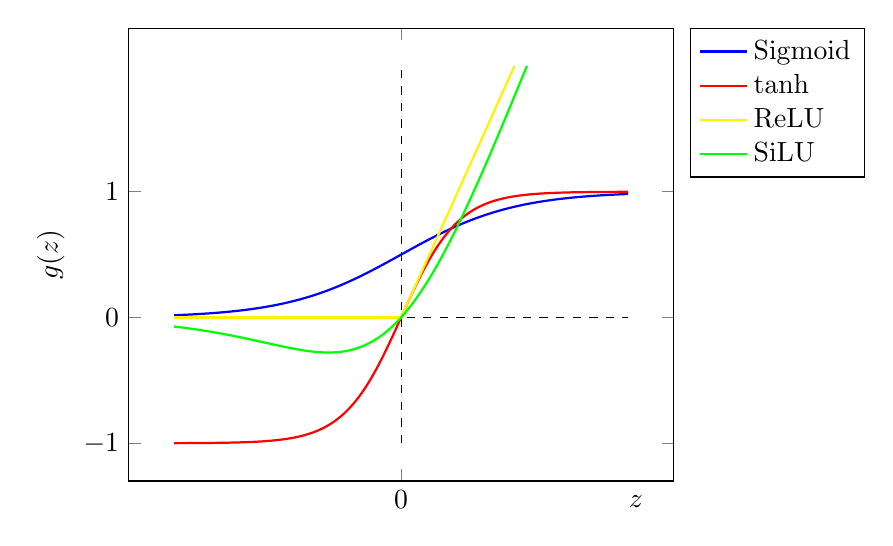
\begin{tikzpicture}
\pgfplotsset{width=8.5cm}
  \begin{axis}[
    domain=-4:4,
    xlabel=$z$,
    ylabel=$g(z)$,
    xtick={0},
    ytick={-1,0,1},
    every axis x label/.style={at={(0.9,-0.01)},anchor=north west},
    legend pos=outer north east,
    legend cell align=left
  ]
  % origin lines
  \addplot +[mark=none, black, dashed, forget plot] coordinates {(-4, 0) (4, 0)};
  \addplot +[mark=none, black, dashed, forget plot] coordinates {(0, -1) (0, 2)};

  % sigmoid 
  \addplot[thick, blue, samples=300] {1/(1+e^(-x))};%
  \addlegendentry{$\textnormal{Sigmoid}$}%

  % tanh
  \addplot[thick, red, samples=300] {tanh(x)};%
  \addlegendentry{$\textnormal{tanh}$}%
  
  % ELU
  %\addplot[thick, blue, samples=300, domain=-4:0, forget plot] {e^x - 1};%
  %\addplot[thick, blue, samples=300, domain=0:2] {x};%
  %\addlegendentry{$\textnormal{ELU}$}%

  % ReLU
  \addplot[thick, yellow, samples=300, domain=-4:0, forget plot] {0};%
  \addplot[thick, yellow, samples=300, domain=0:2] {x};%
  \addlegendentry{$\textnormal{ReLU}$}%

  % swish 
  % 1.278
  % 2.218
  \addplot[thick, green, samples=300, domain=-4:2.218] {x/(1+e^(-x))};%
  \addlegendentry{$\textnormal{SiLU}$}%

  \end{axis}%
\end{tikzpicture}
  \caption{
    The output of several common choices for the activation function $g(z)$ of an artificial neuron.
    The input $z$ is the output of the dot product between the activation and the weights, plus a bias term.
  }
  \label{fig:activation_functions}
\end{figure}


\subsubsection{Networks}

Several neurons are linked together in layers to form a neural network.
The inputs are propagated layer-by-layer through the network until reaching the final output layer.
The number of layers and neurons per layer are important hyperparameters (those parameters which are not optimised as part of the training process) which influence the performance of the model.
In the case of binary classification, the final output layer generally consists of a single neuron with a sigmoid activation 
%
\begin{equation}\label{eq:sigmoid}
  g(z) = \frac{1}{1 + e^{-z}} ,
\end{equation}
%
where $z$ is the output from the dot product of the inputs and the weights, plus the bias term.
The value $g(z)$ is bounded between zero and one allowing the final output to be interpreted as the probability that the input sample belongs to the signal class.
NNs have the crucial property of being differentiable functions, which facilitates the training process described in the next section.

%The activation $a_i^{(l)}$ is the output of the activation function $g(z)$ of the $i^{\text{th}}$ node in layer $l$. The tensor element $\Theta_{ji}^{(l)}$ is the weight connecting the $i^{\text{th}}$ node in layer $l - 1$ to the $j^{\text{th}}$ node in layer $l$. We can compute the outputs for each neuron in a layer simultaneously using ${a}_j^{(l)} = g(\Theta_{ji}^{(l)} a_i^{(l-1)})$, where the activation function is computed element wise on the vector. Computers can perform matrix operations in parallel, making a vectorised implementation such as this more efficient than calculating each output sequentially.

%Taking an item from the dataset $S$, $(\mathbf{x}_i, {y}_i)$, the input $\mathbf{x}_i$ is propagated through the network from left to right, one layer at a time. Finally, the classification result of the network, given by the output of the final neuron $\hat{\mathrm{y}} = h(\mathbf{x}_i)$, is obtained and can be compared to the true category of the data $\mathrm{y}_i$. 



\subsection{Training with Gradient Descent}\label{sec:training_sgd}

A training algorithm is used to optimise the weights and biases of a NN with exposure to the training data.
%The performance of the trained model depends on the amount and quality of the training data, and the efficacy of the training algorithm.
The training algorithm works by minimising a loss function $L$, which quantifies the error in the model's predictions.
NNs are commonly trained using backpropagation in combination with a variant of the stochastic gradient descent algorithm to iteratively update the model parameters.
In binary classification problems, the binary cross entropy loss
%
\begin{equation}\label{eq:bce_loss}
  L(x_i, \theta) = y_i \ln[f_\theta(x_i)] + (1 - y_i) \ln[1 - f_\theta(x_i)],
\end{equation}
%
is often used. Since the model $f$ is differentiable, a correction for each parameter $\theta_i$ can be computed by taking the partial derivative of $L$ with respect to the parameter.
Updated parameters $\theta_i'$ are calculated by updating the original parameter in the direction which reduces the loss.
%
\begin{equation}\label{eq:weight_update}
  \theta_i' = \theta_i - \alpha \pd{L}{\theta_i}
\end{equation}
%
The hyperparameter $\alpha$ is known as the \textit{learning rate} and dictates the size of the step taken in the direction of the slope. 
The errors for each parameter are efficiently calculated using the backpropagation algorithm \cite{rumelhart1986learning}.
The process of updating weights is repeated until the weights are judged to have converged, which means the network is trained.
In practice, small batches of the input data are shown to the network at a time. For each batch the average loss is calculated and the network's weights are updated.
There are many extensions and variations of the gradient descent algorithm.
This work uses the Adam optimiser which adds momentum to the weight updates (dampening oscillations) and an adaptive per-parameter learning rate \cite{2014arXiv1412.6980K}.

\begin{comment}
The gradient descent (\cref{sec:backprop_sgd}) algorithm is used to fit the model to the data.
Using \cref{eq:bce_loss}, an error for 
From \cref{eq:bce_loss}, the error on the output node can be 
The error for the final output node is computed first.
Errors for nodes in the previous layers are computed by \textit{backpropagating} this error through the network.
The error in the output node can be computed explicitly using the loss function in \cref{eq:bce_loss}.
To find the errors for the nodes in the preceding layers $\delta^{(L-1)}_i$, we need to differentiate eq. \ref{neural cost} with respect to $z^{(L-1)}_i$.
In order to perform the differentiation, we relate $z_1^{(L)} = g(z_j^{(L-1)}) \Theta_{1j}^{(L)}$.
The result,is tantamount to propagating the output error back through the network using the weights, and multiplying at each node by the derivative of the activation function. Once the errors have been propagated through the network, the partial derivatives of $J$ can be found using the final expression in eq. \ref{backprop defs}. Lastly the weights are updated simultaneously using eq. \ref{update weights}. 

gradient descent is an example of an \textit{optimisation} algorithm that minimises the cost function $J(\theta)$ (thereby fitting the logistic regression model discussed above to some data) by selecting the optimal values of $\theta$. The algorithm works by computing the partial derivatives of $J(\theta)$ with respect to the parameters $\theta$. The parameters are then altered slightly in the direction of decreasing slope, thereby reducing the cost function.
%The partial derivative of the loss function can be calculated for every parameter $\theta_i$ in the model.

The above step must be performed simultaneously for each $\theta_j$ in $\theta$, after which a new value of $J(\theta)$ can be calculated, and the process repeated. We can compute the partial derivatives of $J$ using the derivative of the logistic function from eq. \ref{eq:bce_loss}. The results are substituted into \cref{eq:weight_update} to obtain
\end{comment}



\section{Track Truth Origin Labelling}\label{sec:track_labelling}

Crucial to supervised learning techniques are the ground truth class labels which the machine learning model is trained to predict.
A set of track truth labels with a sufficient degree of granularity have been implemented in the \ATLAS software stack, and are listed in \cref{tab:truth_origins}.
The labelling scheme has been designed to be useful beyond the classification of good and fake tracks.
The origins are determined by analysing the simulated record to determine the physical process that led to the creation of the truth (i.e. simulated) particle which is  associated with each reconstructed track.
Tracks are associated with truth particles by selecting the particle with the highest \textit{truth-matching probability} (TMP), defined in \cref{eq:tmp_def}.
For a given truth particle, the TMP is a weighted sum of the number of hits on a reconstructed track which are matched to the truth particle $N^{\textnormal{match}}$, divided the total number of hits on the track $N^{\textnormal{total}}$.
The weights are sub-detector-dependent and are designed to account for the varying importance of the different ID sub-detectors (based upon their precision) in the reconstruction of a track.
%
\begin{equation}\label{eq:tmp_def}
    \textnormal{TMP} = 
    \frac{
        10 N_{\textnormal{Pix}}^{\textnormal{match}} + 
        5  N_{\textnormal{SCT}}^{\textnormal{match}} + 
           N_{\textnormal{TRT}}^{\textnormal{match}}
        }{
        10 N_{\textnormal{Pix}}^{\textnormal{total}} + 
        5  N_{\textnormal{SCT}}^{\textnormal{total}} + 
            N_{\textnormal{TRT}}^{\textnormal{total}}
        }
\end{equation}
%
For the fake track classification tool, the track truth origins in \cref{tab:truth_origins} are used to construct a binary label by assigning all fake tracks to the background category, and all other tracks as signal.
The fake track classifier is then trained to distinguish between these two categories of tracks.
Fake tracks are defined using the TMP, with a $\textnormal{TMP} < 0.75$\footnote{An alternative definition of a fake track as one with $\textnormal{TMP} < 0.5$ is also in use within ATLAS, but 0.75 was used for this study.}
giving a track the label of fake.
Fake tracks are made up of combinatorial fakes, which are tracks which do not correspond to the trajectory of any truth particle, and poorly reconstructed tracks, which may somewhat resemble the trajectory of a truth particle but due to the presence of some wrong hits on the track will not accurately reproduce the true trajectory.
In such cases the fake track can still be identified as having an origin: it is for example possible to have a fake track which is from the decay of a \bhadron.


\begin{table}[!htbp]
    \footnotesize\centering
    \setlength{\tabcolsep}{0.5em} % for the horizontal padding
    \begin{tabular}{lll}
        \toprule\hline
        \textbf{Truth Origin} & \textbf{Description} \\
        \hline
        Pile-up  & From a \pp collision other than the primary interaction \\
        Fake    & Created from the hits of multiple particles \\
        Primary & Does not originate from any secondary decay \\
        fromB   & From the decay of a \bhadron \\
        fromBC  & From a \chadron decay which itself is from the decay of a \bhadron \\
        fromC   & From the decay of a \chadron which is not from the decay of a \bhadron \\
        %fromTau & From the decay of a $\tau$ \\
        OtherSecondary & From other secondary interactions and decays \\
        \hline\bottomrule
    \end{tabular}
    \caption{
      Truth origins which are used to categorise the physical process that led to the production of a track.
      Tracks are matched to charged particles using the truth-matching probability~\cite{PERF-2015-08}.
      A truth-matching probability of less than $0.75$ indicates that reconstructed track parameters are likely to be mismeasured and may not correspond to the trajectory of a single charged particle.
      The ``OtherSecondary'' origin includes tracks from photon conversions, \Kshort and $\Lambda^0$ decays, and hadronic interactions.
    }
    \label{tab:truth_origins}
\end{table}

\section{Fake Track Identification Tool}\label{sec:fake_track_mva}

The rate of fake tracks increases at high transverse momentum as shown in \cref{fig:fakerate_vs} due to the difficulties in track reconstruction outlined in \cref{sec:b_had_reco_chall}.
The performance of \btagging algorithms is reduced as a direct result of the presence of these tracks as shown for SV1 (see \cref{sec:vertex_reco}) in \cref{fig:sv1_perf_nofake}, where the efficiency to mistag a \ljet decreases by up to \pct{35} at a \beff of \pct{35} if such tracks are removed.


\begin{figure}[!htbp]
  \centering
  \begin{subfigure}[b]{0.48\textwidth}
      \centering
      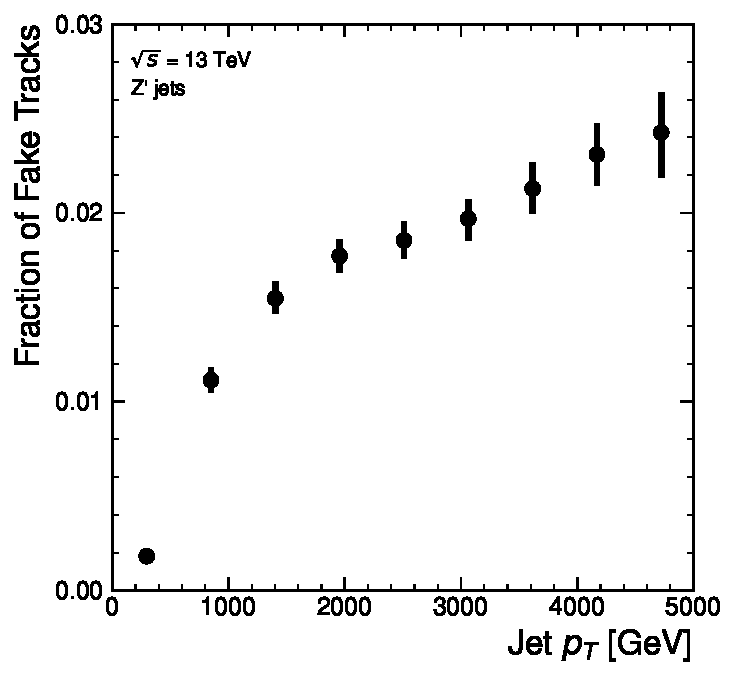
\includegraphics[width=\textwidth]{chapters/4.track_classifier/figs/fake_vs_pt.pdf}
  \end{subfigure}
  \quad
  \begin{subfigure}[b]{0.48\textwidth}
      \centering
      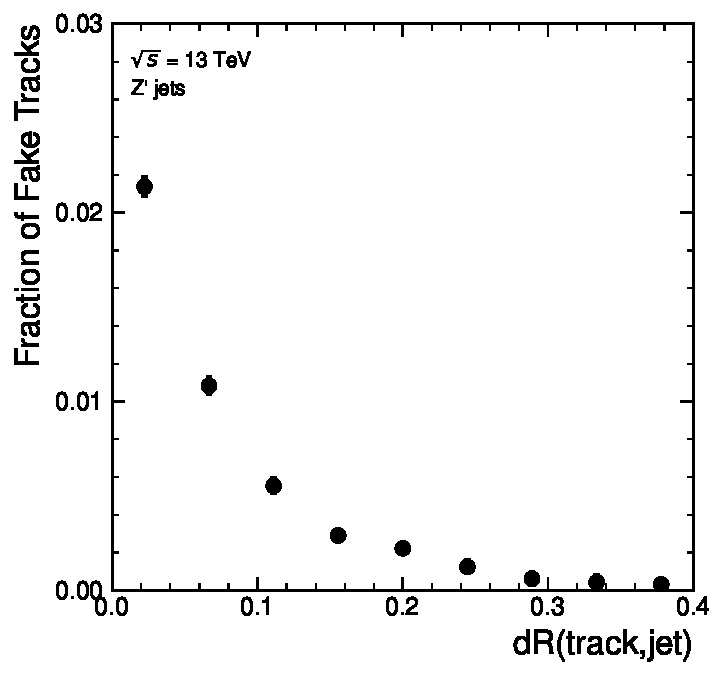
\includegraphics[width=\textwidth]{chapters/4.track_classifier/figs/fake_vs_dr.pdf}
  \end{subfigure}
  \caption{
    Rate of fake tracks as a function of jet transverse momentum (left) and $\DeltaR(\textnormal{track}, \textnormal{jet})$ (right) for jets in the \Zprime sample.
    The rate of fake tracks increases significantly as a function of \pt, and also increases as the distance to the jet axis decreases.
  }
  \label{fig:fakerate_vs}
\end{figure}

\begin{figure}[!htbp]
    \centering
    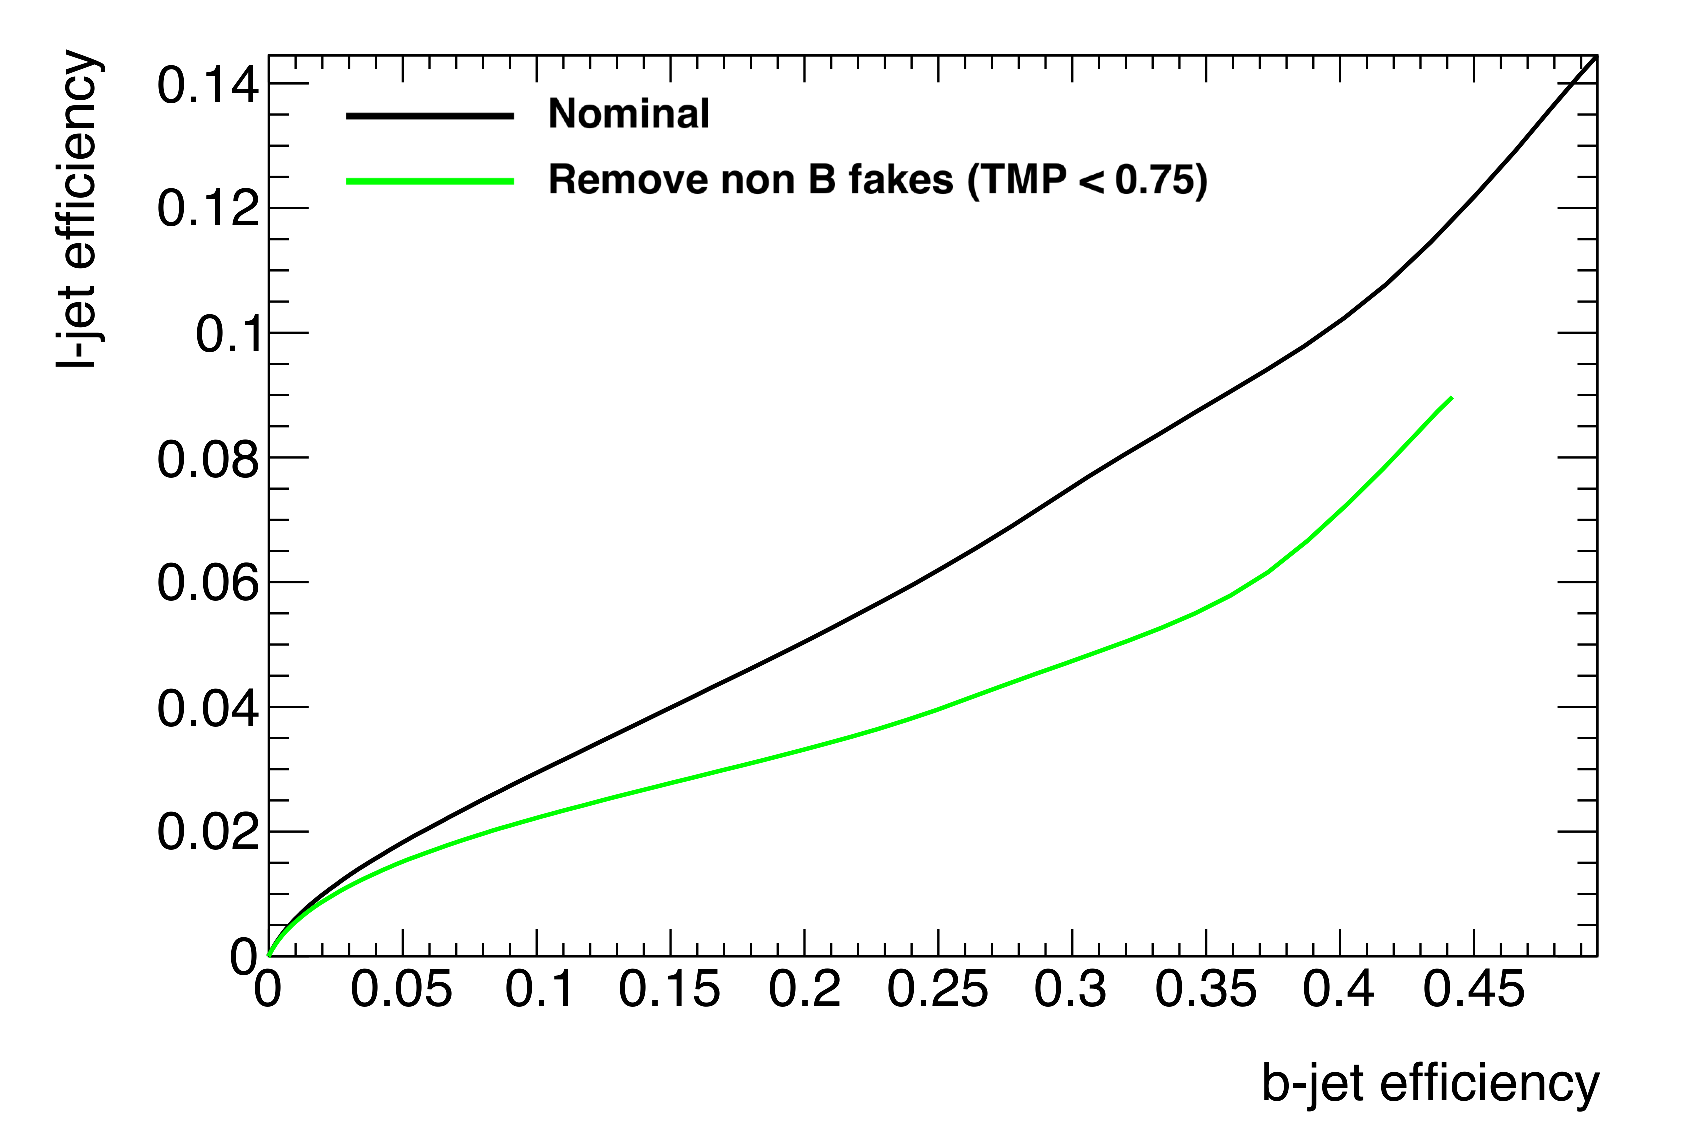
\includegraphics[width=0.7\textwidth]{chapters/4.track_classifier/figs/sv1_perf_nofake.pdf}
    \caption{
      The \ljet efficiency of the low level tagger SV1 for \Zprimejets with \Zprimept, as a function of \bjet efficiency.
      The nominal tracking setup (black) is shown alongside the case where fake tracks which are not from the decay of a \bhadron are removed.
      The \ljet efficiency is decreased, demonstrating that the presence of fake tracks is detrimental to the algorithm performance.
    }
    \label{fig:sv1_perf_nofake}
\end{figure}

To identify and remove fake tracks, a NN classification tool was trained with all non-fake tracks as the signal class and fake tracks as the background class.
Inputs to the model are described in \cref{sec:fake_mva_model_inputs}, while fake track removal performance is given in \cref{sec:fake_track_mva_results}.
Both models are trained and evaluated using tracks associated to jets from the \ttbar and \Zprime samples described in \cref{sec:track_classifier_datasets}.
\ttbarjets made up \pct{70} of the jets used for training, with the remaining \pct{30} coming from \Zprimejets.


\subsection{Model Inputs}\label{sec:fake_mva_model_inputs}

%\newcommand{\ipdefsfootnote}{%
%Impact parameter significances are defined as the IP divided by its corresponding uncertainty, $\dzerosig = d_0 / \dzerouncert$ and $\zzerosig = z_0 / \zzerouncert$.
%Track IP significances are lifetime signed according to the track's direction with respect to the jet axis and the primary vertex \cite{PERF-2012-04}.
%}

The fake track NN is given two jet variables and 20 tracking related variables for each track fed into the network.
The jet transverse momentum and signed pseudorapidity constitute the jet-level inputs, with the track-level inputs listed in \cref{tab:fake_mva_track_inputs}.


\begin{table}[!htbp]
  \footnotesize\centering
  \setlength{\tabcolsep}{0.5em} % for the horizontal padding
  \begin{tabular}{ll}
    \toprule\hline
    \textbf{Jet Input} & \textbf{Description} \\
    \hline
    $\pt$ & Jet transverse momentum \\
    $\eta$ & Signed jet pseudorapidity \\
    \toprule
    \textbf{Track Input} & \textbf{Description} \\
    \hline
    $\pt$ & Track transverse momentum \\
    $\DeltaR$ & Angular distance between the track and jet \\
    $d_0$  & Closest distance from the track to the PV in the longitudinal plane \\
    $z_0$  & Closest distance from the track to the PV in the transverse plane \\
    nIBLHits   & Number of IBL hits \\
    nPixHits   & Number of pixel hits \\
    nSCTHits   & Number of SCT hits \\
    nTRTHits   & Number of TRT hits \\
    nBLHits    & Number of B-layer hits \\
    nIBLShared & Number of shared IBL hits \\
    nIBLSplit  & Number of split IBL hits \\
    nPixShared & Number of shared pixel hits \\
    nPixSplit  & Number of split pixel hits \\
    nSCTShared & Number of shared SCT hits \\
    $r_{\textnormal{first}}$      & Radius of first hit \\
    nDOF   & Number of degrees of freedom on the track \\
    FracRank & Ambiguity solver ordering variable \\
    \hline\bottomrule
  \end{tabular}
  \caption{
    Input features to the fake track classification NN.
    Basic jet kinematics, along with information about the reconstructed track parameters and constituent hits are used.
    Shared hits, are hits used on multiple tracks which have not been classified as split by the cluster-splitting neural networks~\cite{PERF-2015-08}, while split hits are hits used by multiple tracks which have been identified as merged, and therefore split.
    ``Primary vertex'' (defined in \cref{sec:vertex_reco}) is abbreviated as PV.
  }
  \label{tab:fake_mva_track_inputs}
\end{table}

The track parameters and hit pattern are key indicators of whether or not a track is fake.
The FracRank variable is the ordered index of the tracks that pass the ambiguity solver's selection divided by the total number of successfully reconstructed tracks in the event.
The ambiguity solver processes track candidates iteratively in order of an internal score (see \cref{sec:track_reco}), and the order in which tracks are accepted is preserved.
Since tracks with shared hits have lower scores, tracks which do not require the removal of shared hits are likely to be processed and accepted earlier on, whereas tracks with shared hits will be processed later and potentially have their shared hits removed.
Hence the FracRank variable gives an indication of the track quality and how likely it is that hits would have been removed (tracks processed later on are more likely to have hits removed).

Track selection follows the loose selection described in \rcite{ATL-PHYS-PUB-2020-014} and outlined in \cref{tab:fake_track_mva_selections}, which was found to improve the performance compared to previous tighter selections, whilst ensuring good resolution of the track's parameters and a low fake rate \cite{PERF-2015-08}.
Inputs are scaled to have a central value of zero and a variance of unity before training and evaluation.


\subsection{Model Hyperparameters}\label{sec:hyperparameters}

Due to the imbalance between the two classes (with fake tracks being relatively uncommon), a weight was added to the loss function for the background class to balance their relative weights.
The NN was made up of two hidden layers with 220 nodes per layer.
The ReLU activation function was used in conjunction with the Adam optimiser with a learning rate of $1\text{e}{-3}$.
Optimisation of the networks architecture was carried out to ensure optimal performance with a relatively small number of learnable parameters -- 54,000.
The model was trained using \num{40} million tracks with a further \num{4} million tracks each used for validation and testing.
The number of tracks used for training was found to be sufficient to maximise the performance of the model, with no improvement observed when using more tracks.
A full list of the model hyperparameters is given in \cref{tab:fake_track_mva_hyperparams}.

\begin{table}[!htbp]
  \footnotesize\centering
  \setlength{\tabcolsep}{0.5em} % for the horizontal padding
  \begin{tabular}{lll}
      \toprule\hline
      \textbf{Hyperparameter} & \textbf{Value} \\
      \hline
      Batch size & 2048 \\
      Activation & ReLU \\
      Optimiser & Adam \\
      Initial learning rate & $1\text{e}{-3}$ \\
      Training epochs & 20 \\
      Training tracks & 40m \\
      Validation tracks & 4m \\
      Testing tracks & 4m \\
      \hline\bottomrule
  \end{tabular}
  \caption{
    Hyperparameters for the track classification model.
  }
  \label{tab:fake_track_mva_hyperparams}
\end{table}


\subsection{Results}\label{sec:fake_track_mva_results}


In order to evaluate the fake track classification tool, a orthogonal test sample of $4$ million tracks in jets in the combined \ttbar and \Zprime samples was used.
The continuous scalar output from the NN model is interpreted as the probability that a given track is a signal track (i.e. not fake).
\cref{fig:track_classifier_output_roc} shows the performance of the fake track classification NN. The signal and background classes are well separated in the output of the tool.
Also shown is a receiver operating characteristic (ROC) curve, which plots the rate of true positives against the rate of false positives over a scan of cut points on the NN output ranging from zero to one.
The area under the curve (AUC) gives a summary of the aggregate classification power of the model.
The fake track classification tool achieves an AUC of $0.935$ for all tracks, which is indicative of a well-performing model.
Considering only tracks from \bhadron decays, this value drops slightly to $0.928$. 

\begin{figure}[!htbp]
  \centering
  \begin{subfigure}[b]{0.48\textwidth}
      \centering
      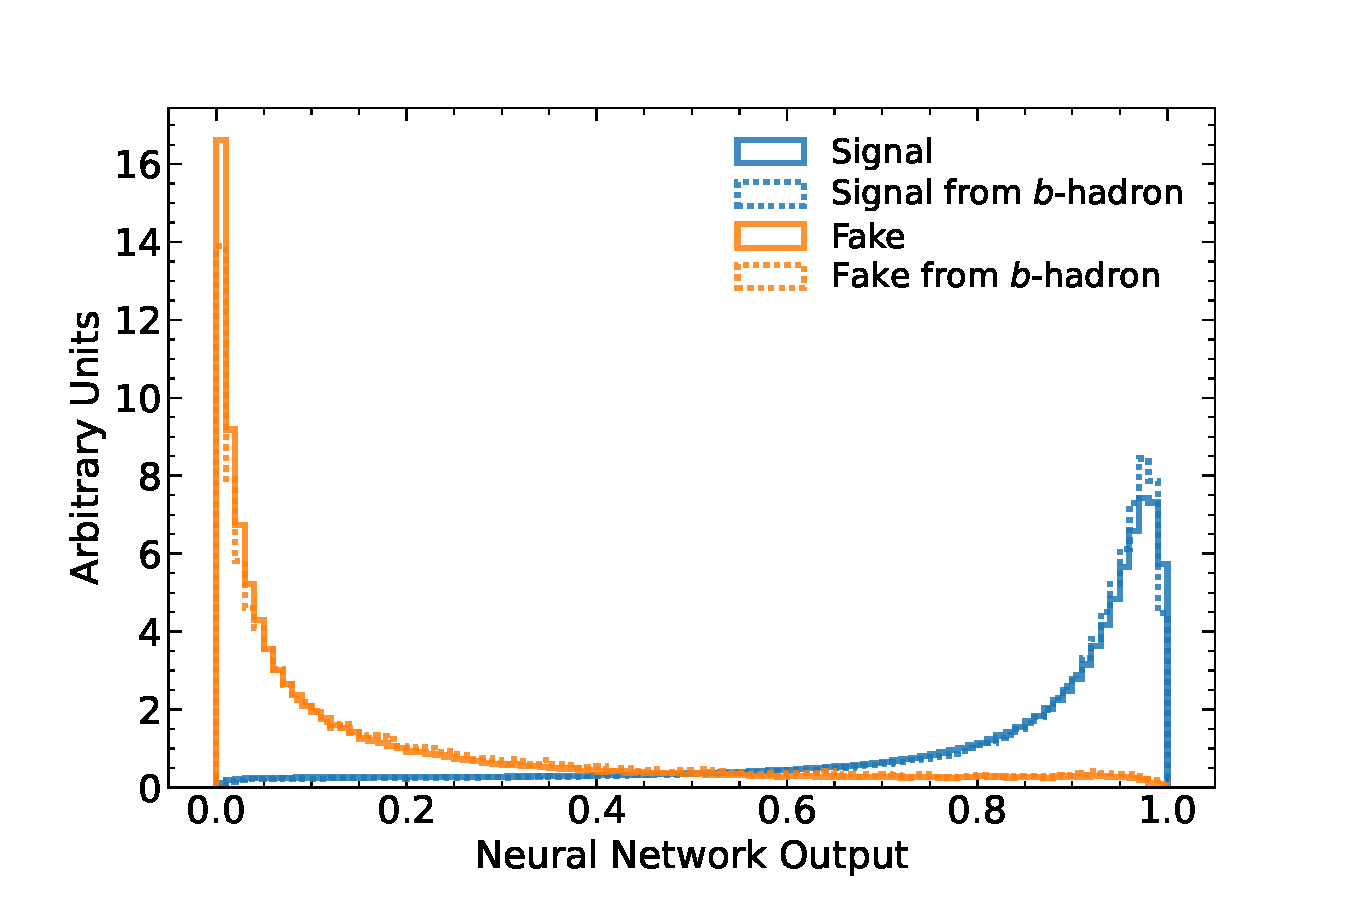
\includegraphics[width=\textwidth]{chapters/4.track_classifier/figs/fake_id_output.pdf}
  \end{subfigure}
  \quad
  \begin{subfigure}[b]{0.48\textwidth}
      \centering
      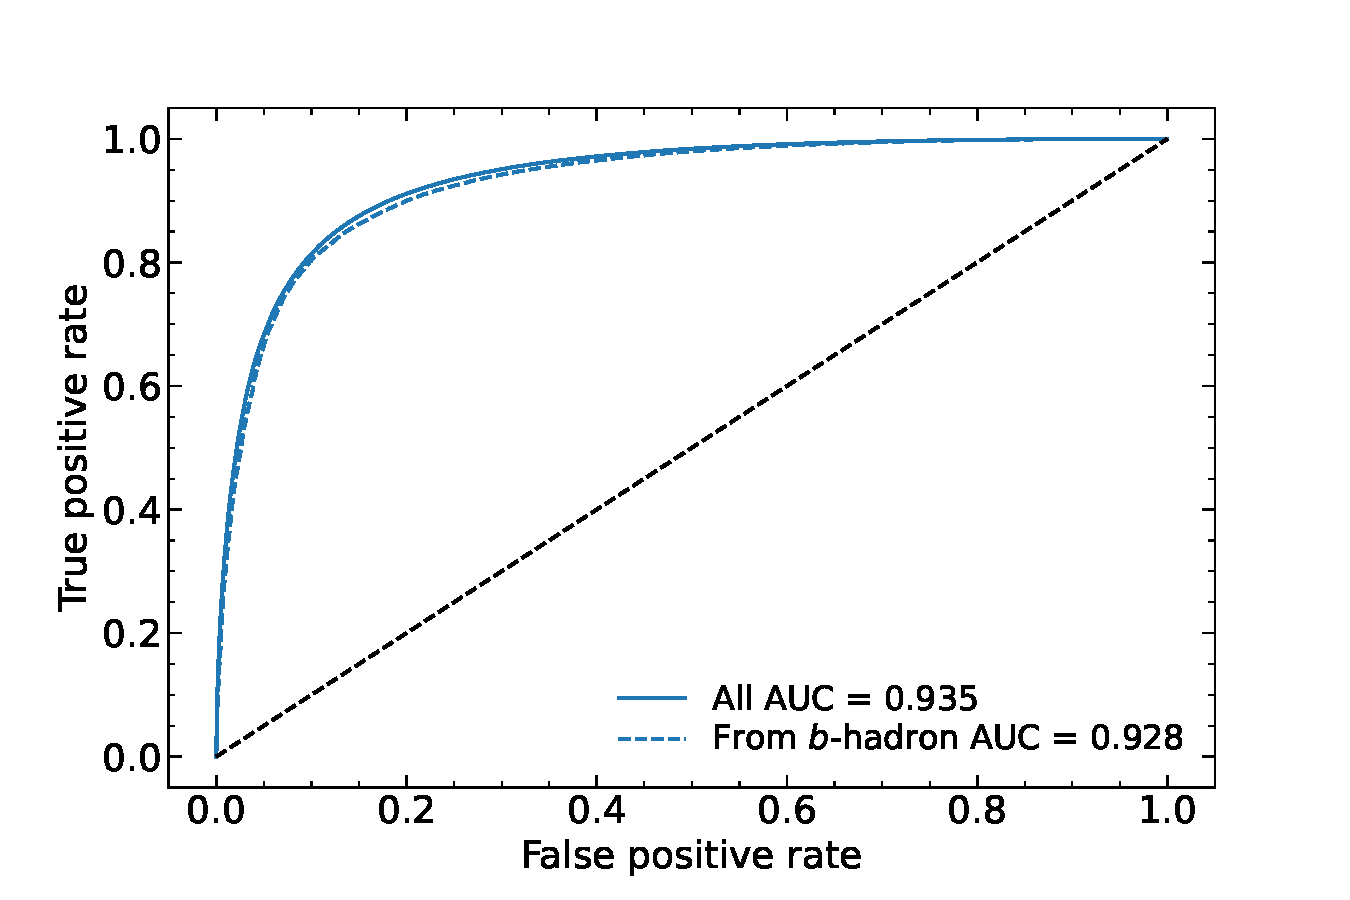
\includegraphics[width=\textwidth]{chapters/4.track_classifier/figs/fake_id_roc.pdf}
  \end{subfigure}
  \caption{
    (left) Normalised histograms of the fake track classification model output separated for signal and fake tracks, and further separated by those tracks which are from the decay of a \bhadron.
    (right) The ROC curve for all tracks (solid line) and tracks from the decay of a \bhadron (dashed line).
    The plots show tracks in the combined \ttbar and \Zprime testing sample.
    The model is able to successfully discriminate between signal and fake tracks, and shows a very similar performance when looking specifically at tracks from the decay of a \bhadron.
  }
  \label{fig:track_classifier_output_roc}
\end{figure}

Signal and fake track efficiencies at two different NN output cut points are shown in \cref{tab:fake_track_mva_effs}.
The results demonstrate that the tool is effective in retaining \pct{98.8} of signal tracks, while correctly identifying (and therefore enabling the removal of) \pct{45.6} of fake tracks.
\cref{tab:fake_track_mva_effs} also shows that a significant amount of tracks which are labelled as both fake and from the decay of a \bhadron are also removed.
This can happen because fake tracks with $\textnormal{TMP} < 0.75$ are still matched to a truth particle, which can be the decay product of a \bhadron.

\begin{table}[!htbp]
  \footnotesize\centering
  \setlength{\tabcolsep}{0.5em} % for the horizontal padding
  \begin{tabular}{ccccc}
      \toprule\hline
      \multirow{2}{2cm}{NN Output Cut} & \multicolumn{2}{c}{\textbf{Signal Track Efficiency}} & \multicolumn{2}{c}{\textbf{Fake Track Recall}} \\
      & All & From $b$ & All & From $b$ \\
      \hline
      0.06 & \pct{98.8} & \pct{98.9} & \pct{45.6} & \pct{39.8} \\
      0.12 & \pct{97.3} & \pct{97.5} & \pct{59.4} & \pct{53.6} \\
      \hline\bottomrule
  \end{tabular}
  \caption{
    Good and fake track selection efficiencies for the combined \ttbar and \Zprime samples.
    Two working points are defined, cutting on the NN output at $0.06$ and $0.12$.
  }
  \label{tab:fake_track_mva_effs}
\end{table}

\section{\bhadron Track Identification}

After initial tests and investigation, it was found that fake tracks which were the result of \bhadron decays actually aided \btagging performance, as demonstrated in \cref{fig:track_mva_sv1}.
The application of a single tool which removed all fake tracks was therefore not optimal.
A second tool was therefore trained in the same manner as the first, this one was designed to distinguish between those tracks which were from the decay of a \bhadron (FromB and FromBC in \cref{tab:truth_origins}) and those which were not (all other truth origins).
Fake tracks which were from the decay of a \bhadron were included in the signal class.
The \bhadron decay track NN was trained using the same setup as described above, with the same tracks, input variables, and training procedure.
The performance of the model to separate \bhadron decay tracks from other tracks is shown in \cref{fig:b_id_output_roc}.
Using a selection WP of 0.1, the model can retain \pct{98.5} of \bhadron tracks and reject \pct{46.2} of tracks not from the decay of a \bhadron.
In \cref{sec:mva_combined}, this model is used in conjunction with the fake track identification NN to identify and remove fake tracks which are not from the decay of a \bhadron.

% TODO: ADD TABLE REQUEST 

\begin{figure}[!htbp]
  \centering
  \begin{subfigure}[b]{0.48\textwidth}
      \centering
      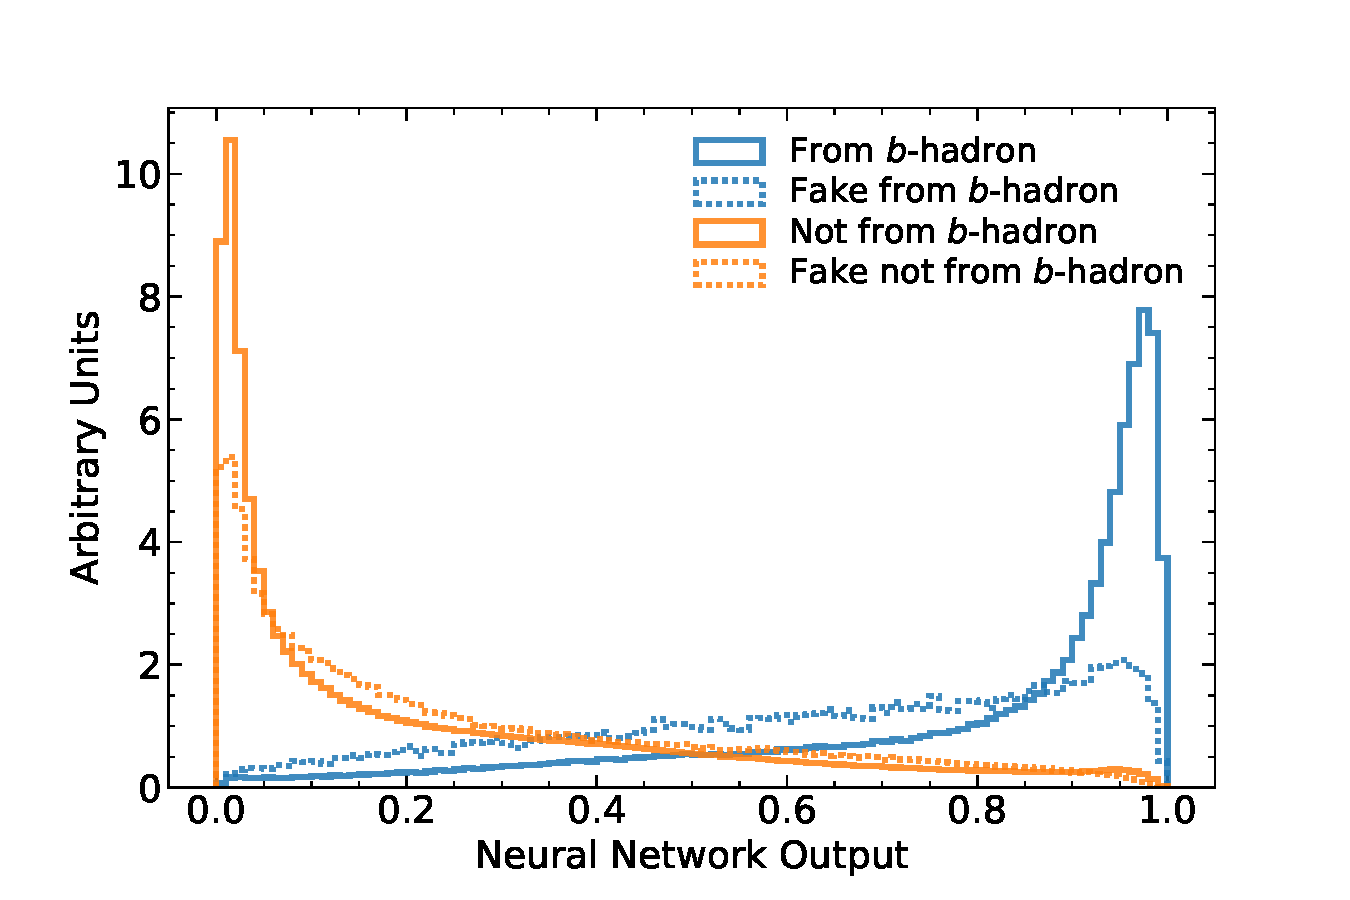
\includegraphics[width=\textwidth]{chapters/4.track_classifier/figs/b_id_output.pdf}
  \end{subfigure}
  \quad
  \begin{subfigure}[b]{0.48\textwidth}
      \centering
      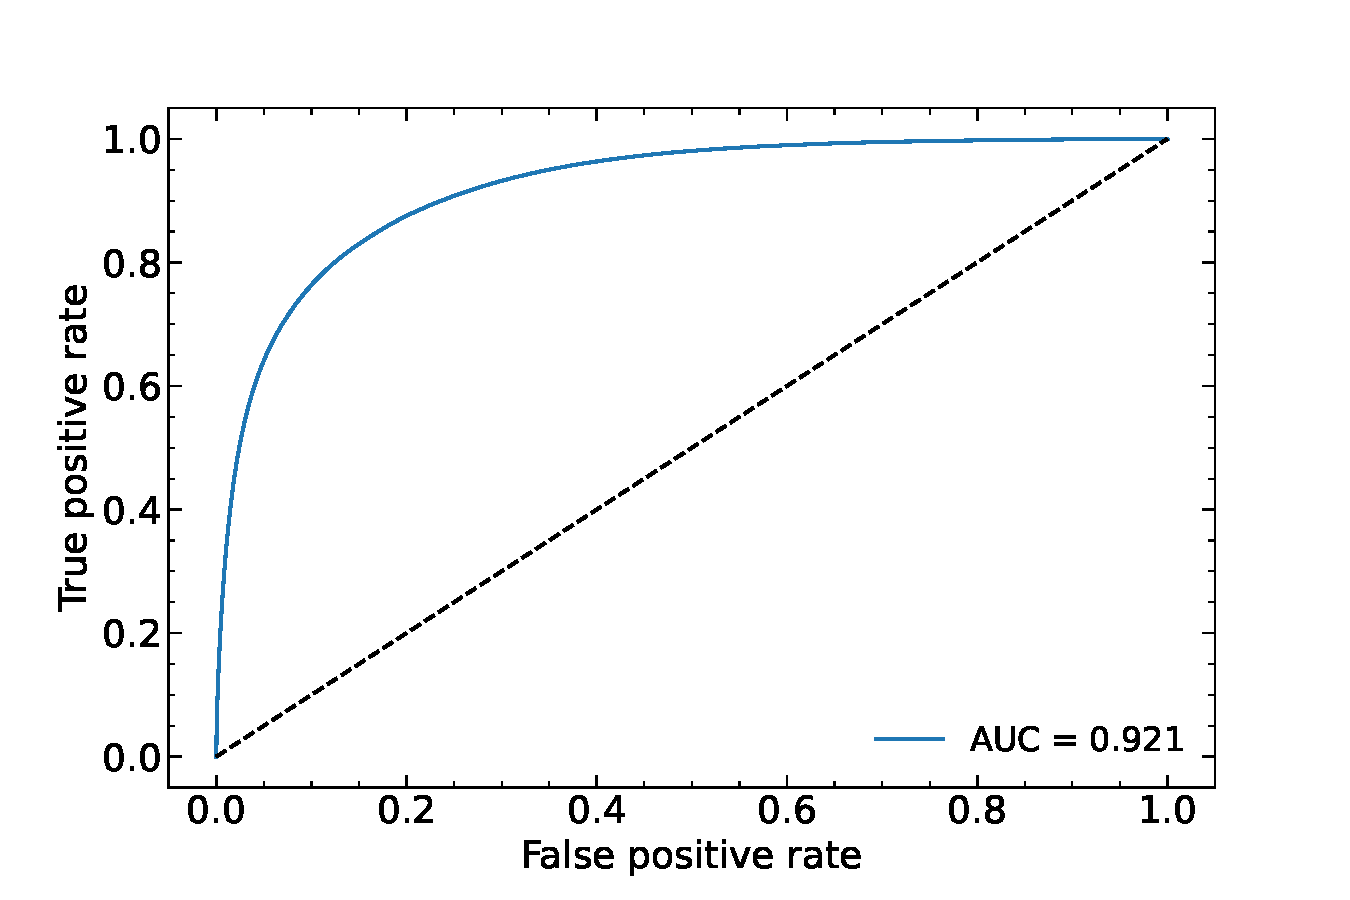
\includegraphics[width=\textwidth]{chapters/4.track_classifier/figs/b_id_roc.pdf}
  \end{subfigure}
  \caption{
    (left) Normalised histogram of the \bhadron track identification model output separated for tracks from the decay of a \bhadron and tracks from other sources.
    The two groups are further separated into those tracks which are fake.
    (right) The ROC curve for all tracks (solid line).
    The plots show tracks in the combined \ttbar and \Zprime testing sample.
  }
  \label{fig:b_id_output_roc}
\end{figure}


\section{Combined Approach}\label{sec:mva_combined}


A 2-dimensional cut was then used to only reject those tracks that had a high probability of being fake, and also a low probability of being a \bhadron decay track.
The results of the combined approach are provided in \cref{tab:combined_va}, which shows that for the working point ``A'', \pct{98.6} of \bhadron decay tracks (both good and fake) are retained, while \pct{50.7} of fake tracks which are not from \bhadron decays are rejected.

\begin{table}[!htbp]
  \footnotesize\centering
  \setlength{\tabcolsep}{0.5em} % for the horizontal padding
  \begin{tabular}{l>{\raggedright}p{2cm}>{\raggedright}p{2cm}>{\raggedright}p{4cm}>{\raggedright\arraybackslash}p{4cm}}
      \toprule\hline
      \textbf{WP} & \textbf{Fake NN Cut} & \textbf{\bhadron Decay NN Cut} & \textbf{Retained \bhadron Tracks} & \textbf{Fake non-\bhadron Tracks Rejected} \\
      \hline
      A & 0.5 & 0.4 & \pct{98.6} & \pct{50.7} \\
      B & 0.6 & 0.5 & \pct{97.5} & \pct{62.0} \\
      \hline\bottomrule
  \end{tabular}
  \caption{
    Cut values for the fake and \bhadron decay track NNs for the two defined working points.
    Working point ``B'' cuts more aggressively on the NN outputs than WP ``A'', removing more fake tracks but resulting in an increased loss of signal tracks (which here are all \bhadron decay tracks).
  }
  \label{tab:combined_va}
\end{table}
%// cut A: B tracks kept = 98.6% (99.4% of good B tracks and 84.8% of fake B tracks). Non B Fakes Rejected: 50.7%
%// cut B: B tracks kept = 97.5% (98.4% of good B tracks and 80.8% of fake B tracks). Non B Fakes Rejected: 62.0%

The \ljet efficiency of SV1 is successfully reduced when using the combined tools to remove fake tracks that are not from a \bhadron decay, as shown in \cref{fig:track_mva_sv1}.
At a \beff of \pct{70}, the \ljet mistag rate for jets with $250 < \pt < \SI{400}{\GeV}$ is reduced from $0.054$ to $0.044$, a relative improvement of approximately \pct{20}.
For jets with $400 < \pt < \SI{1000}{\GeV}$ the mistag rate drops from 0.1 to 0.08 for a similar relative improvement of \pct{20}.
The performance of the fake track removal approach was also tested for the other low level vertexing algorithm -- JetFitter.
A similar level of improvement in the \ljet mistag rate was observed with a reduction of up to a \pct{20} reduction for both low- and \highpt \Zprimejets achieved.
Together, these results demonstrate that by identifying and removing fake tracks which are not the result of the weak decay of a \bhadron, the performance of the low level tagging algorithms can be improved by an amount which is comparable to the improvement that would be observed if the tracks were selected at truth level1.

\begin{figure}[!htbp]
  \centering
  \begin{subfigure}[b]{0.48\textwidth}
      \centering
      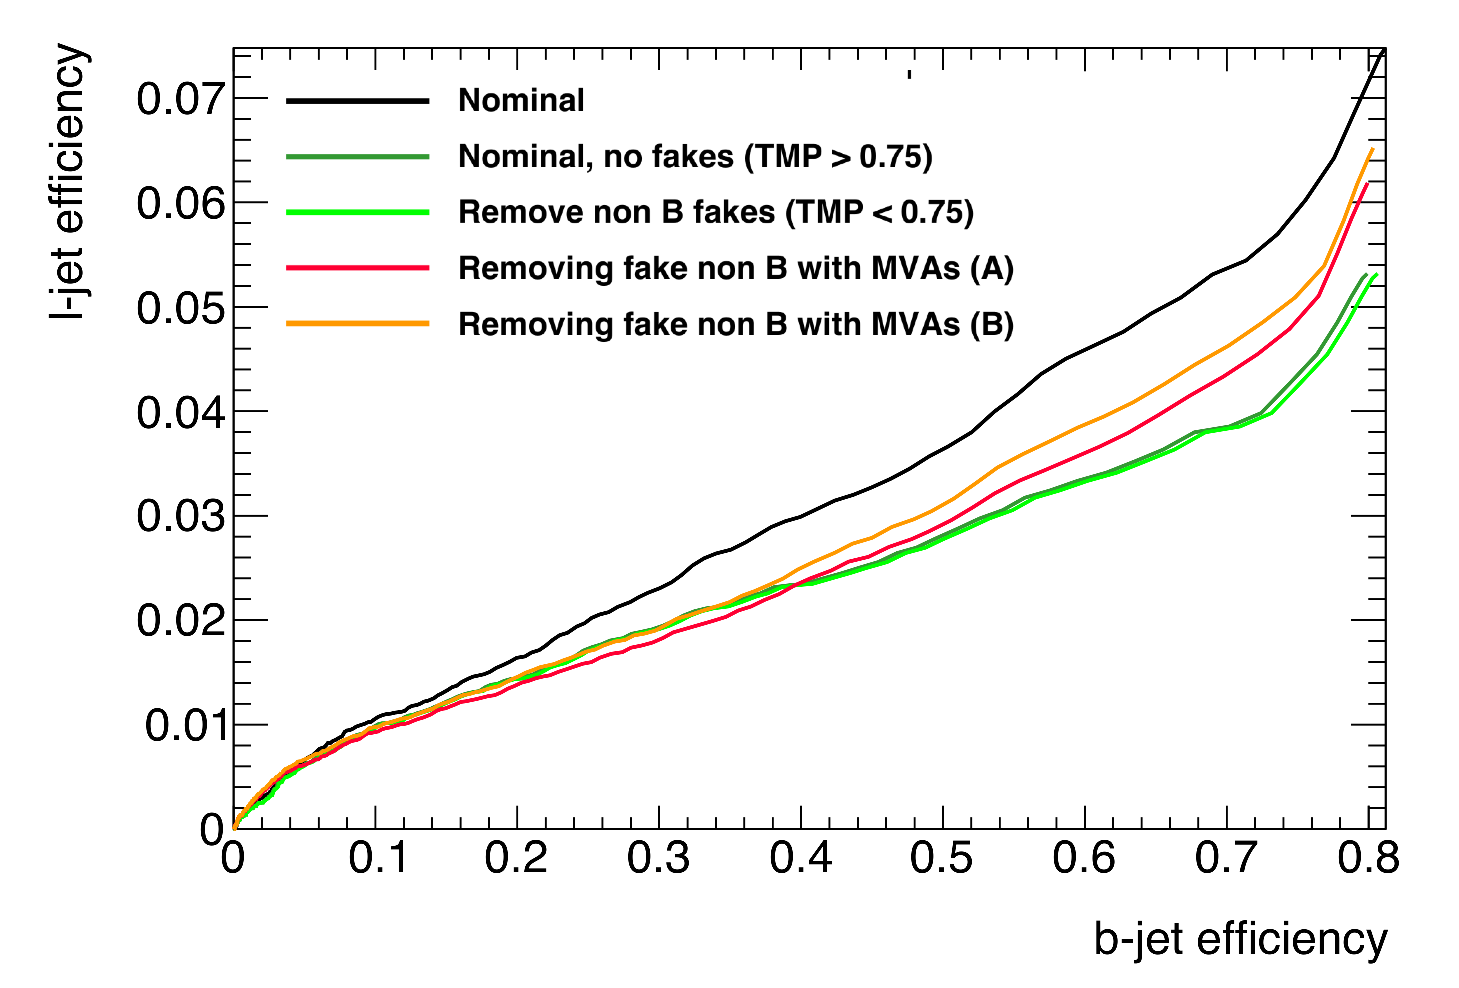
\includegraphics[width=\textwidth]{chapters/4.track_classifier/figs/sv1_mva_lowpt.pdf}
  \end{subfigure}
  \quad
  \begin{subfigure}[b]{0.48\textwidth}
      \centering
      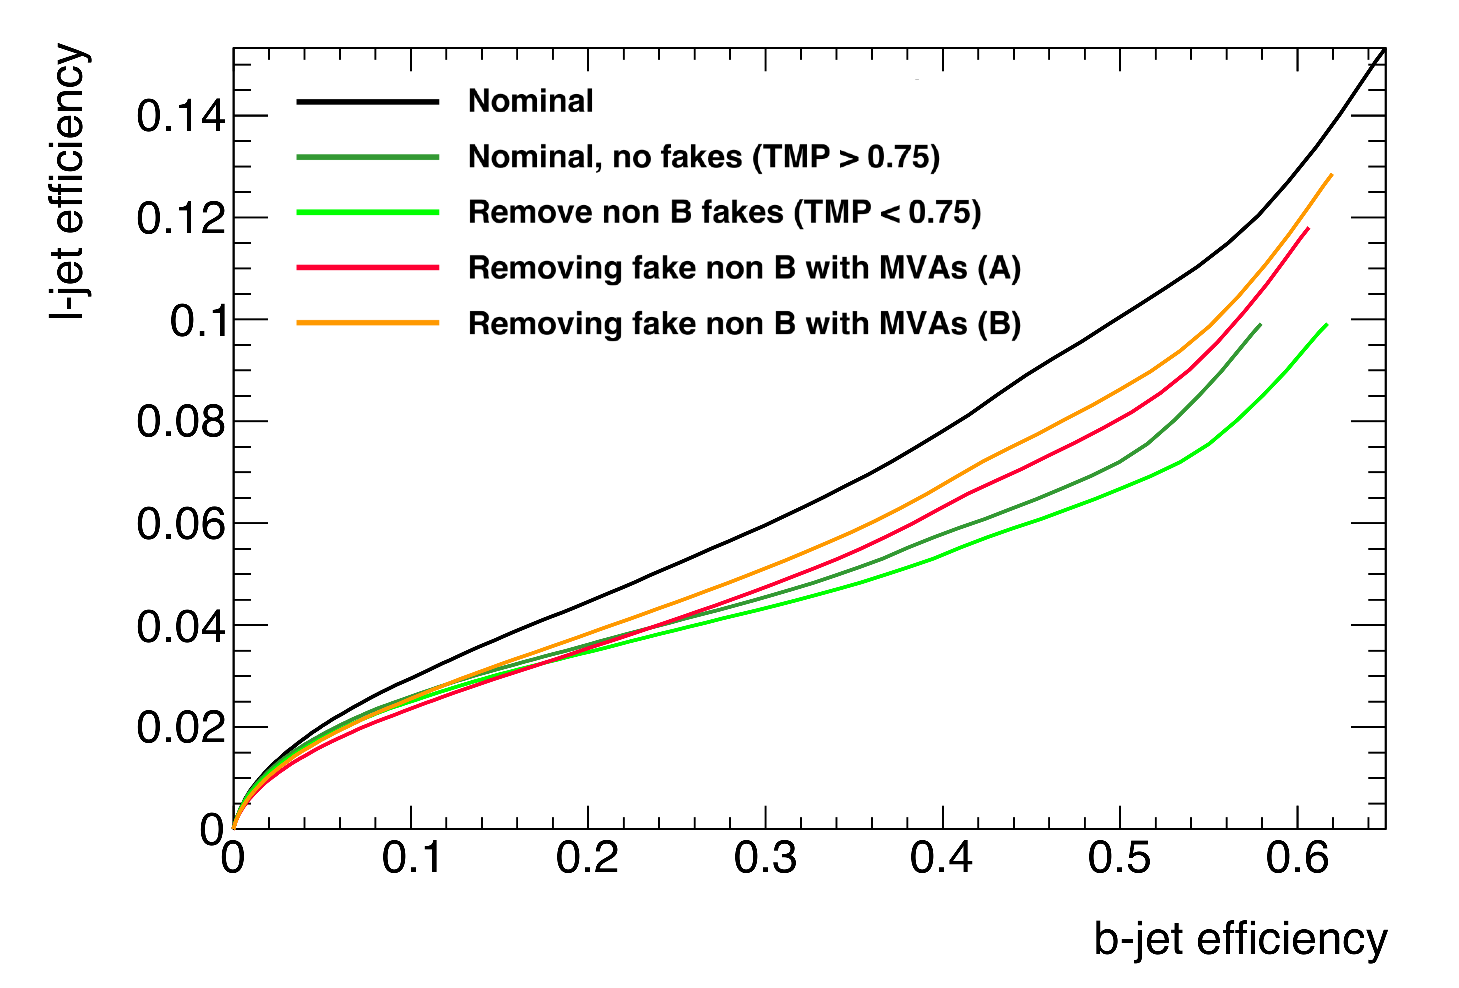
\includegraphics[width=\textwidth]{chapters/4.track_classifier/figs/sv1_mva_hipt.pdf}
  \end{subfigure}
  \caption{
    The effect of applying the fake track identification algorithm together with the \bhadron decay track identification on the jet tagging performance of SV1 for \Zprimejets with $\SI{250}{\GeV} < \pt < \SI{400}{\GeV}$ (left) and $\SI{400}{\GeV} < \pt < \SI{1}{\TeV}$ (right).
    The nominal SV1 \ljet efficiency (black) is compared to two working points of fake track removal, labelled ``A'' (red) and ``B'' (orange), which represent two different 2D working points of the track classification tools.
    Removal of fake tracks based on truth information is shown by the green curves.
  }
  \label{fig:track_mva_sv1}
\end{figure}

%\begin{figure}[!htbp]
%  \centering
%  \begin{subfigure}[b]{0.48\textwidth}
%      \centering
%      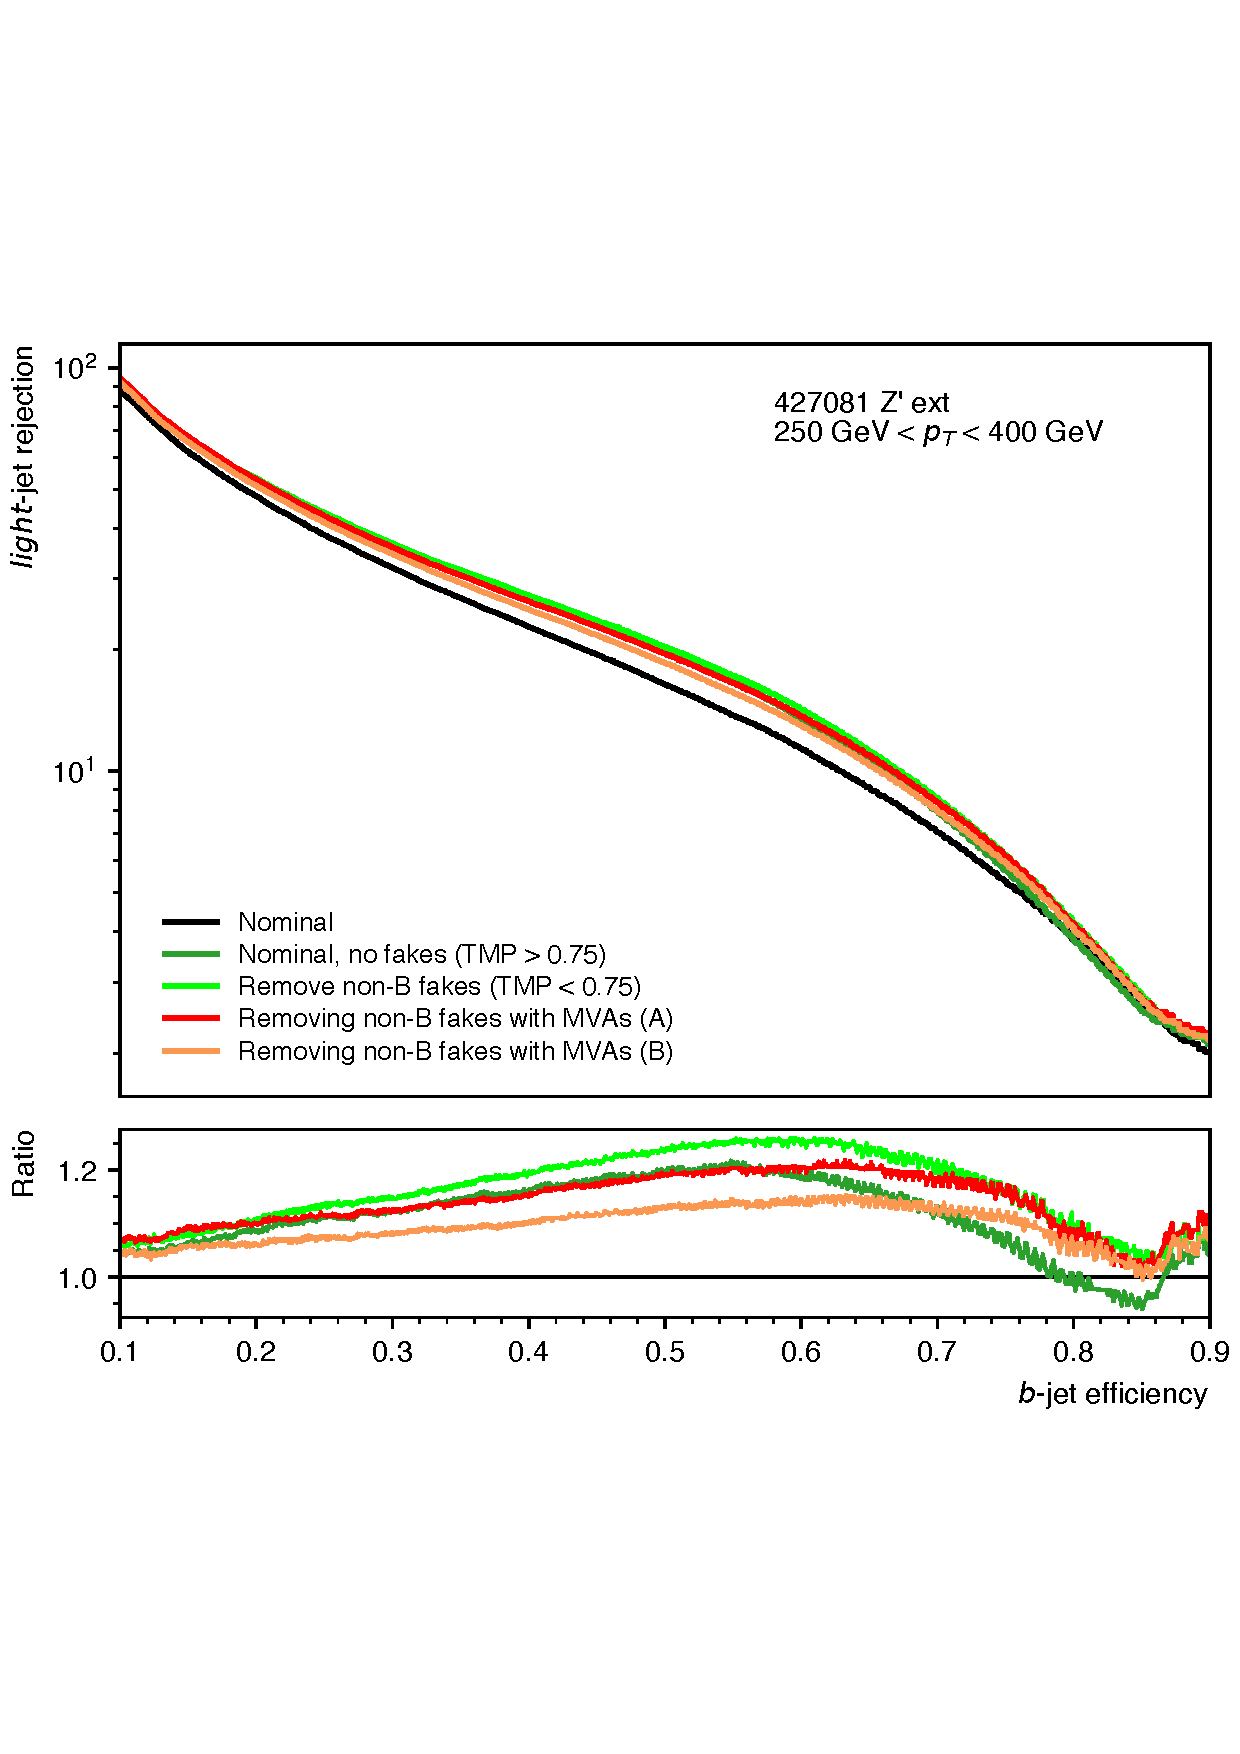
\includegraphics[width=\textwidth]{chapters/4.track_classifier/figs/zprime_jf_lowpt.pdf}
%  \end{subfigure}
%  \quad
%  \begin{subfigure}[b]{0.48\textwidth}
%      \centering
%      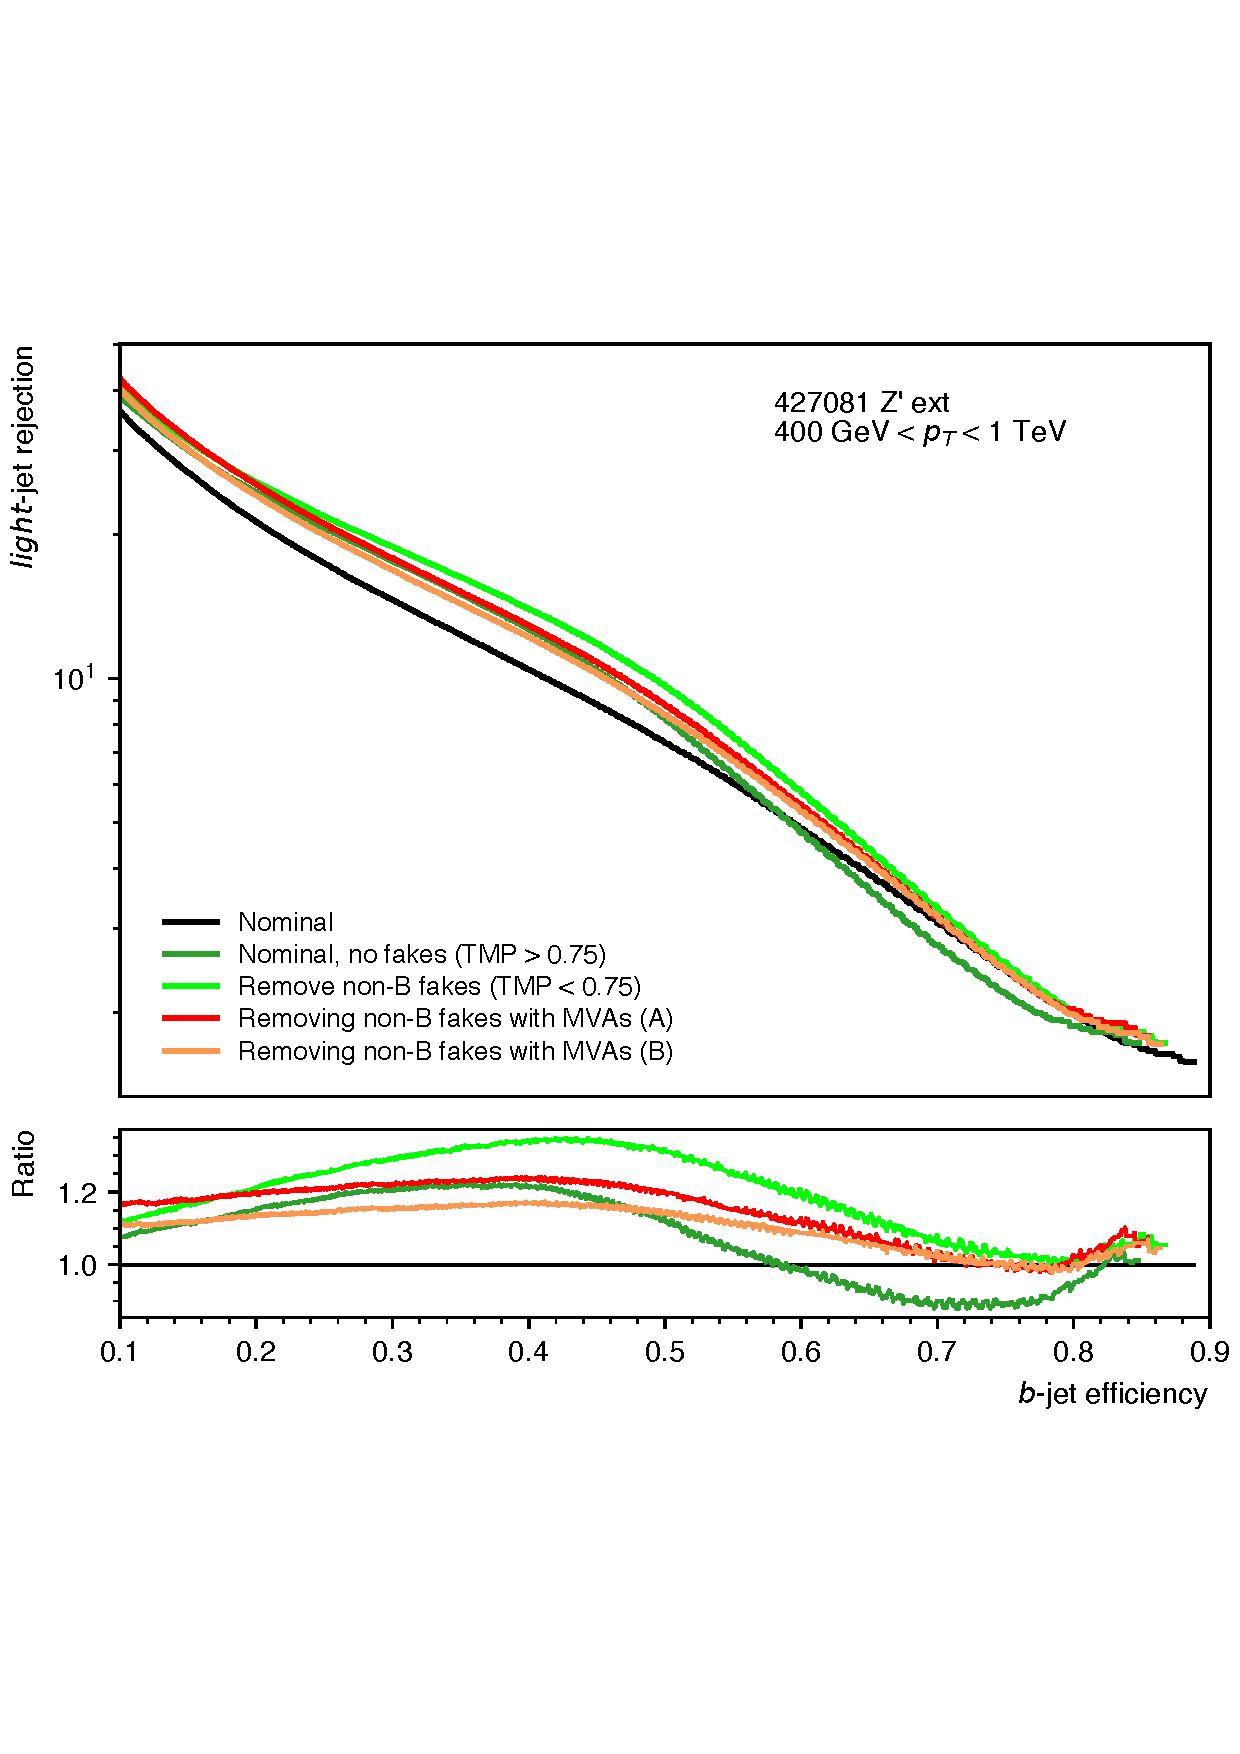
\includegraphics[width=\textwidth]{chapters/4.track_classifier/figs/zprime_jf_highpt.pdf}
%  \end{subfigure}
%  \caption{
    %The effect of applying the fake track identification algorithm alongside the \bhadron decay track identification on the jet tagging performance of JetFitter for jets with $\SI{250}{\GeV} < \pt < \SI{400}{\GeV}$ (left) and for jets with $\SI{400}{\GeV} < \pt < \SI{1}{\TeV}$ (right).
%    The nominal JetFitter \lrej (black) is compared to two working points of fake track removal, labelled ``A'' (red) and ``B'' (orange).
%    Removal of fake tracks based on truth information is shown by the green curves.
%  }
%  \label{fig:track_mva_jf}
%\end{figure}



\section{Conclusion}\label{sec:fake_track_mva_conclusion}

Fake tracks, which are prevalent in the core of high \pt jets, have an adverse impact on the performance of the low-level \btagging algorithms SV1 and JetFitter.
A ML tool to identify fake tracks has been developed.
The tool can be used to limit the number of fake tracks being input to the low-level tagging algorithms.
An advantage of the approach is that the continuous output of the model allows for the tuning of good and fake track identification efficiencies.
Since it was found that \bhadron decay tracks can also be poorly reconstructed and thus marked as fake, it was deemed necessary also to train a second algorithm to detect \bhadron decay tracks so that the removal of these tracks could be avoided.
Removing fake and non-$b$ decay tracks in this way was found to improve the \ljet mistagging rate of SV1 and JetFitter by up to \pct{20} at high transverse momentum.
The improvement achieved using the classification tools was generally comparable with that achieved when using the truth information to remove the fake tracks not from the decay of a \bhadron, demonstrating the efficacy of the approach.

\subsubsection{Future Work}
While removing tracks prior to their input to the low level tagging algorithms is shown here to be beneficial, a more performant alternative might be to keep these tracks but label them as being fake (for example using the output of the classification tool), and allow the tagging algorithms to take this into consideration.
This is not straightforward with manually optimised low-level taggers such as SV1 and JetFitter, but is possible with more advanced taggers as described in \cref{chap:gnn_tagger}.

Tools which identify the origin of a given track have other potential uses.
One application is to isolate a relatively pure sample of fake tracks which can be used to estimate the fake track rate in data, which would be useful for estimating the uncertainty on fake track modelling.
Another application is to use the \bhadron track identification tool to improve the track-to-jet association.
Both applications are currently under investigation within \ATLAS.

The approach here works on a track-by-track basis, but a more sophisticated approach would consider the correlations between the tracks inside a jet.
Also left for future work is to simultaneously train a single tool which discriminates between all the truth origins listed in \cref{tab:truth_origins}.
Such a tool would be useful as a general purpose track origin classifier.
An algorithm which takes both these aspects into consideration is discussed in \cref{chap:gnn_tagger}.

  \chapter{Graph Neural Network Flavour Tagger}\label{chap:gnn_tagger}

Some of the work in this chapter has previously been published in \rcite{ATL-PHYS-PUB-2022-027}.
The author of this thesis was on the editorial team.
Figures, tables and text from the published note are reproduced here.

Flavour tagging, the identification of jets originating from \bcquarks, is a critical component of the physics programme of the ATLAS experiment at the Large Hadron Collider. 
Current flavour tagging algorithms rely on the outputs of several low-level algorithms, which reconstruct various properties of jets using charged particle tracks, that are then combined using machine learning techniques.
In this note a new machine learning algorithm based on graph neural networks, \GNN, is introduced.
\GNN uses information from a variable number of charged particle tracks within a jet, to predict the jet flavour without the need for intermediate low-level algorithms.
Alongside the jet flavour prediction, the model predicts which physics processes produced the different tracks in the jet, and groups tracks in the jet into vertices.
These auxiliary training objectives provide useful additional information on the contents of the jet and improve performance.
\GNN compares favourably with the current ATLAS flavour tagging algorithms.
For a \bjet efficiency of \pct{70}, the light ($c$)-jet rejection is improved by a factor of \ttbllo (\ttbclo) for jets coming from \ttbar decays with transverse momentum \ttbarpt.
For jets coming from \Zprime decays with transverse momentum \Zprimept, the light ($c$)-jet rejection improves by a factor \zpbllo (\zpbclo) for a comparative \pct{30} \bjet efficiency.


\section{Motivation}\label{sec:gnn_motvation}


\newcommand{\fakesfootnote}{%
A fake track is defined as a track with a truth-matching probability less than $0.5$, where the truth-matching probability is defined in Ref.~\cite{PERF-2015-08}.
}

Flavour tagging, the identification of jets originating from \bcquarks, is a critical component of the physics programme of the ATLAS experiment~\cite{PERF-2007-01} at the Large Hadron Collider (LHC)~\cite{Evans:2008zzb}.
It is of particular importance for the study of the Standard Model (SM) Higgs boson and the top quark, which preferentially decay to \bquarks \cite{HIGG-2018-04,HIGG-2018-13}, and additionally for several Beyond Standard Model (BSM) resonances that readily decay to heavy flavour quarks \cite{EXOT-2019-03}.
The significant lifetime of \bhadrons, approximately $\SI{1.5}{\ps}$ \cite{PhysRevD.98.030001}, provides the unique signature of a secondary decay vertex which has a high mass and is significantly displaced from the primary vertex. Additional signatures of \bhadrons are the tertiary decay vertex, resulting from $b \rightarrow c$ decay chains, and the reconstructed trajectories of charged particles (henceforth simply referred to as tracks) with large impact parameters\footnote{The distance of closest approach from a track to the primary vertex.} (IPs).
These signatures are primarily identified using tracks associated to jets. As such, efficient and accurate track reconstruction is essential for high performance flavour tagging.

This note introduces a novel algorithm, \GNN, which uses Graph Neural Networks (GNNs)~\cite{battaglia2018relational} with auxiliary training objectives, to aid the primary goal of classifying whether jets originate from \ensuremath{b\text{- or }c\text{-quarks}}\xspace(referred to as a flavour tagger). %to identify \ensuremath{b\text{- or }c\text{-jets}}\xspace, . 
The concept is illustrated in \cref{fig:oldvsnew}.
The use of GNNs offers a natural way to classify jets with variable numbers of unordered associated tracks, while allowing for the inclusion of auxiliary training objectives \cite{2020-gnn-for-sv,serviansky2020set2graph}.

\begin{figure}[!htbp]
    \centering
    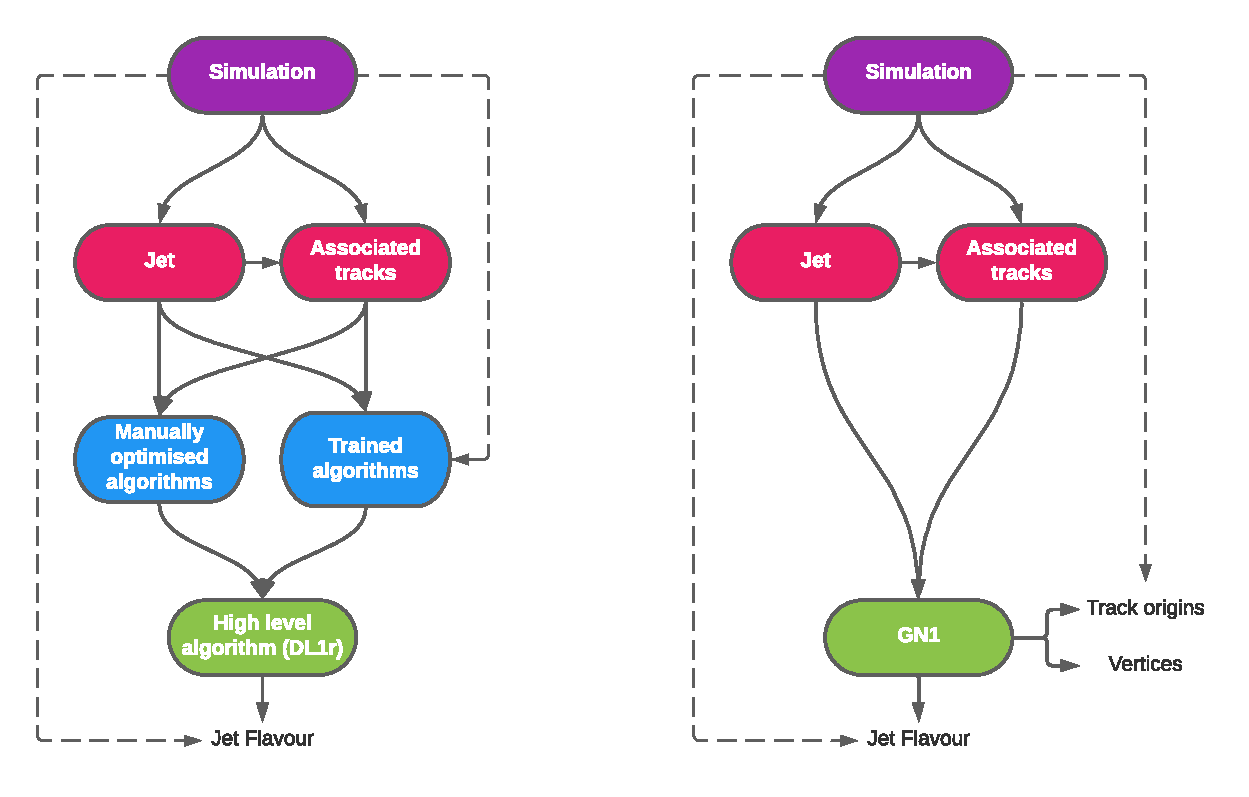
\includegraphics[width=0.8\linewidth]{chapters/gnn_tagger/figs/GNN_compare_contrast.pdf}
    \caption{Comparison of the existing flavour tagging scheme (left) and \GNN (right). The existing approach utilises low-level algorithms (shown in blue), the outputs of which are fed into a high-level algorithm (\DLr). Instead of being used to guide the design of the manually optimised algorithms, additional truth information from the simulation is now being used as auxiliary training targets for \GNN. The solid lines represent reconstructed information, whereas the dashed lines represent truth information.}
    \label{fig:oldvsnew}
\end{figure}

The current ATLAS flavour tagger, \DLr \cite{ATL-PHYS-PUB-2017-013}, is a deep neural network which takes the outputs of a number of independently optimised ``low-level'' algorithms \cite{FTAG-2018-01} as inputs. 
Each of these low-level algorithms makes use of tracks to reconstruct a particular aspect of the experimental signature of heavy flavour jets.
%, for example the presence of secondary vertices (those caused by displaced decays of heavy flavour hadrons).
The low-level algorithms can be manually optimised reconstruction algorithms, for example the SV1 and JetFitter algorithms that reconstruct displaced decay vertices, or trained taggers such as RNNIP and DIPS that use the IPs of a variable number of tracks to identify the flavour of the jet \cite{FTAG-2018-01,ATL-PHYS-PUB-2017-011,ATL-PHYS-PUB-2017-003,ATL-PHYS-PUB-2020-014}.
In contrast \GNN utilises a single neural network, which directly takes the tracks and some information about the jet as inputs. As such, it does not depend on any other flavour tagging algorithm, and a single training of the \GNN fully optimises all aspects of the algorithm.  

\GNN is trained to understand the internal structure of the jet through the use of two auxiliary training objectives: the grouping of tracks originating from a common vertex, and the prediction of the underlying physics process from which each track originated.
These auxiliary objectives are meant to guide the neural network towards a more complete understanding of the underlying physics, removing the need for the low-level algorithms, and therefore simplifying the process of optimising the tagger for new regions of phase space (e.g. \ctag or high-\pt \btag), or when the detector or charged particle reconstruction algorithms are updated.
The training targets for the primary and auxiliary objectives are extracted from “truth information”, i.e. information only available in simulation, as opposed to reconstructed quantities available in both collision data and simulation.

In this note, the following benefits of this approach will be shown:

\begin{enumerate}
    \item Improved performance with respect to the current ATLAS flavour tagging algorithms, with larger background rejection for a given signal efficiency.
    \item The same network architecture can be easily optimised for a wider variety of use cases (e.g. \cjet tagging and high-\pt jet tagging), since there are no low-level algorithms to retune.
    \item There are fewer flavour tagging algorithms to maintain.
    \item Alongside the network's prediction of the jet flavour, the auxiliary vertex and track origin predictions provide more information on why a jet was (mis)tagged or not. This information can also have uses in other applications, for instance to explicitly reconstruct displaced decay vertices or to remove fake tracks.\footnote{\fakesfootnote}
\end{enumerate}

This note is organised as follows: a brief description of the ATLAS detector, object definitions and selections, and samples are provided in \cref{sec:experimental_setup}; details about the model architecture and training procedure are given in \cref{sec:networks}; and results are discussed in \cref{sec:gnn_results}.


\section{Graph Neural Network Theory}\label{sec:gnn_theory}



\section{Experiemental Setup}\label{sec:experimental_setup}

\subsection{Datasets}\label{sec:datasets}

Datasets used to train the \GNN tagger are the same as described in \cref{sec:track_classifier_datasets}.

As previously, truth labelled \bcl jets are kinematically re-sampled in \pt and $\eta$ to ensure identical distributions in these variables. 
The resulting dataset contains \njetstrain jets, \pct{60} of which are \ttbar jets and \pct{40} of which are \Zprime jets.
While \DLr uses \pct{70} \ttbar jets and \pct{30} \Zprime jets, the change in sample composition did not affect the final performance of \GNN.
To evaluate the performance of the model, \njetsval jets from both the \ttbar and \Zprime samples, which are statistically independent from the training sample, are used. 
Track- and jet-level inputs are scaled to have a central value of zero and a variance of unity before training and evaluation. 


\section{Model Architecture}\label{sec:networks}

\subsection{Model Inputs}\label{sec:model-inputs}

\newcommand{\ipdefsfootnote}{%
Impact parameter significances are defined as the IP divided by its corresponding uncertainty, $\dzerosig = d_0 / \dzerouncert$ and $\zzerosig = z_0 / \zzerouncert$.
Track IP significances are lifetime signed according to the track's direction with respect to the jet axis and the primary vertex \cite{PERF-2012-04}.
}

\GNN is given two jet variables and 21 tracking related variables for each track fed into the network.
The jet transverse momentum and signed pseudorapidity constitute the jet-level inputs, with the track-level inputs listed in \cref{tab:track_inputs}.
If a jet has more than 40 associated tracks, the first 40 tracks with the largest transverse IP significance\footnote{\ipdefsfootnote} \dzerosig are selected as inputs.
Full track parameter information and associated uncertainties, along with detailed hit information, carry valuable information about the jet flavour.
In the dense cores of high-\pt jets, tracks are highly collimated and separation between tracks can be of the same order as the active sensor dimensions, resulting in merged clusters and tracks which share hits \cite{PERF-2015-08}.
Due to the relatively long lifetimes of \bhadrons and \chadrons, which can traverse several layers of the ID before decaying and have highly collimated decay products, the presence of shared or missing hits is a critical signature of heavy flavour jets.
Full track parameter information and associated uncertainties, along with detailed hit information, carry valuable information about the jet flavour.

Dependence on the absolute value of the azimuthal jet angle $\phi$ is explicitly removed by providing only the azimuthal angle of tracks relative to the jet axis. The track pseudorapidity is also provided relative to the jet axis.

Since heavy flavour hadrons can decay semileptonically, the presence of a reconstructed lepton in the jet carries discriminating information about the jet flavour.
In addition to the baseline \GNN model, the \GNNLep variant includes an additional track-level input, leptonID, which indicates if the track was used in the reconstruction of an electron, a muon or neither. %has a value of $\pm 11$ ($\pm 13$) if the track was used in the reconstruction of an electron (muon), and $0$ otherwise.
The muons are required to be combined \cite{ATL-PHYS-PUB-2015-037}, and the electrons are required to pass the \textit{VeryLoose} likelihood-based identification working point \cite{PERF-2017-01}.

\begin{table}[!htbp]
  \footnotesize\centering
  \setlength{\tabcolsep}{0.5em} % for the horizontal padding
  \begin{tabular}{ll}
    \toprule\hline 
    \textbf{Jet Input} & \textbf{Description} \\
    \hline
    $\pt$ & Jet transverse momentum \\
    $\eta$ & Signed jet pseudorapidity \\
    \toprule
    \textbf{Track Input} & \textbf{Description} \\
    \hline
    $q/p$ & Track charge divided by momentum (measure of curvature) \\
    $\mathrm{d}\eta$ & Pseudorapidity of the track, relative to the jet $\eta$ \\
    $\mathrm{d}\phi$  & Azimuthal angle of the track, relative to the jet $\phi$ \\
    $d_0$  & Closest distance from the track to the PV in the longitudinal plane \\
    $z_0 \sin\theta$  & Closest distance from the track to the PV in the transverse plane \\
    $\sigma(q/p)$ & Uncertainty on $q/p$ \\
    $\sigma(\theta)$ & Uncertainty on track polar angle $\theta$ \\
    $\sigma(\phi)$  & Uncertainty on track azimuthal angle $\phi$ \\
    $\dzerosig$  & Lifetime signed transverse IP significance \\
    $\zzerosig$  & Lifetime signed longitudinal IP significance \\
    nPixHits   & Number of pixel hits \\
    nSCTHits   & Number of SCT hits \\
    nIBLHits   & Number of IBL hits \\
    nBLHits    & Number of B-layer hits \\
    nIBLShared & Number of shared IBL hits \\
    nIBLSplit  & Number of split IBL hits \\
    nPixShared & Number of shared pixel hits \\
    nPixSplit  & Number of split pixel hits \\
    nSCTShared & Number of shared SCT hits \\
    nPixHoles  & Number of pixel holes \\
    nSCTHoles  & Number of SCT holes \\
    leptonID   & Indicates if track was used to reconstruct an electron or muon \\
    \hline\bottomrule
  \end{tabular}
  \caption{
    Input features to the \GNN model.
    Basic jet kinematics, along with information about the reconstructed track parameters and constituent hits are used.
    Shared hits, are hits used on multiple tracks which have not been classified as split by the cluster-splitting neural networks~\cite{PERF-2015-08}, while split hits are hits used on multiple tracks which have been identified as merged.
    A hole is a missing hit, where one is expected, on a layer between two other hits on a track.
    The track leptonID is an additional input to the \GNNLep model.
  }
  \label{tab:track_inputs}
\end{table}

Track selection follows the loose selection used for the fake track classification MVA in \cref{chap:track_classification_mva} and described in \cref{tab:fake_track_mva_selections}.
This selection was found to improve the flavour tagging performance compared to previous tighter selections, whilst ensuring good resolution of tracks and a low fake rate~\cite{PERF-2015-08}.
\cref{sec:looser_track_selection} demonstrates that further relaxation of the track selection requirements may be warranted. 


\subsection{Auxiliary Training Objectives}\label{sec:aux-train-objectives}

In addition to the jet flavour classification, two auxiliary training objectives are defined.
Each auxiliary training objective comes with a training target which, similar to the jet flavour label, are truth labels derived from the simulation.
The presence of the auxiliary training objectives improves the jet classification performance as demonstrated in \cref{sec:gnn_ablations}.

The first auxiliary objective is the prediction of the origin of each track within the jet. 
Each track is labelled with one of the exclusive categories defined in \cref{tab:truth_origins} after analysing the particle interaction that led to its formation. 
Since the presence of different track origins is strongly related to the flavour of the jet, training \GNN to recognise the origin of the tracks may provide an additional handle on the classification of the jet flavour.
This task may also aid the jet flavour prediction by acting as a form of supervised attention~\cite{arxiv.2007.08294}~-~in detecting tracks from heavy flavour decays the model may learn to pay more attention to these tracks.

Displaced decays of \bchadrons lead to secondary and tertiary vertices inside the jet.
Displaced secondary vertices can also occur in \ljets as a result of material interactions and long-lived particle decays (e.g. \Kshort and $\Lambda^0$).
The second auxiliary objective is the prediction of track-pair vertex compatibility. 
For each pair of tracks in the jet, \GNN predicts a binary label, which is given a value 1 if the two tracks in the pair originated from the same point in space, and 0 otherwise. 
To derive the corresponding truth labels for training, truth production vertices within $0.1$ mm are merged.
%, as these are assumed to be unresolvable given the granularity of the ID. 
Track-pairs where one or both of the tracks in the pair have an origin label of either Pileup or Fake are given a label of 0.
Using the pairwise predictions from the model, collections of commonly compatible tracks can be grouped into vertices.
%Two existing low-level tagging algorithms, SV1 and JetFitter, are currently used to find and reconstruct vertices inside jets.
The addition of this auxiliary training objective removes the need for inputs from a dedicated secondary vertexing algorithm.

Both auxiliary training objectives can be considered as ``stepping stones'' on the way to classifying the flavour of the jet. 
By requiring the model to predict the truth origin of each track and the vertex compatibility of each track-pair, the model is guided to learn representations of the jet which are connected to the underlying physics and therefore relevant for classifying the jet flavour. 


%\begin{figure}[!htbp]
%    \centering
%    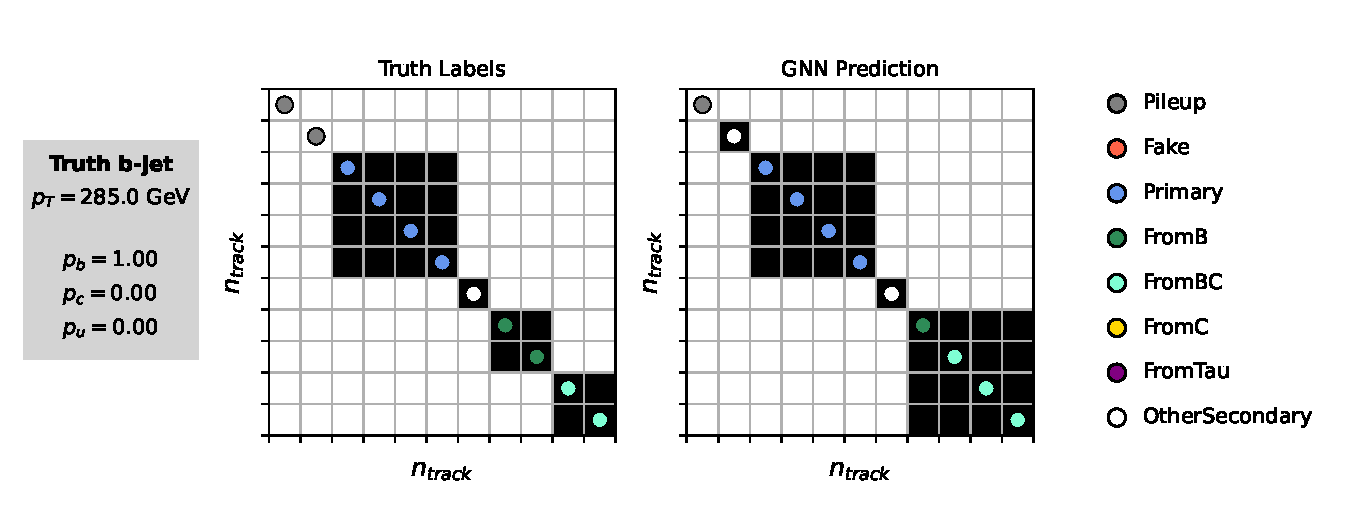
\includegraphics[width=\textwidth]{chapters/gnn_tagger/figs/results/jet_view_1.pdf}
    %\caption{Truth (left) and predicted (right) structure of a \bjet. The shaded black boxes show the grouping of tracks into vertices. In this example, \GNN correctly groups the four primary tracks as having come from a common origin, but does not resolve the $B \rightarrow D$ hadron vertex decay chain. One of the pileup tacks is misidentified as a being OtherSecondary, and one of the $b$ decay tracks is misidentified as being from a $b \rightarrow c$ hadron decay. Nevertheless \GNN correctly predicts the flavour of the jet with a high degree of certainty (class probabilities $p_b$, $p_c$ and $p_u$ are rounded to three significant figures).}
%    \label{fig:jet_view_1}
%\end{figure}
%The auxiliary training objectives also allow for improved model interpretability. 
%\cref{fig:jet_view_1} shows a comparison of the truth origin and vertex information compared with the predicted values from \GNN.
%Such comparisons indicate that \GNN recovers the indended representation of the jet structure, and can also be used to identify limitations.


\subsection{Architecture}\label{sec:Architecture}

As discussed above, the \GNN model combines a graph neural network architecture~\cite{2020-gnn-in-particle-physics} with auxiliary training objectives in order to determine the jet flavour.
Coarse optimisation of the network architecture hyperparameters, for example number of layers and number of neurons per layer, has been carried out to maximise the tagging efficiency.

The model architecture is based on a previous implementation of a graph neural network jet tagger~\cite{serviansky2020set2graph}.
As compared to the previous approach, \GNN uses a only a single graph neural network and makes use of a more sophisticated graph neural network layer \cite{2021arXiv210514491B}, described below.
These changes yield improved tagging performance and a significant reduction in training time with respect to the previous approach.
%the auxiliary classification tasks are performed at the end, along with the graph classification, as opposed to being run half way through the moel and then being fed back in.
%The previous architecture differs from the newer in that it is comprised two graph networks, whereas the newer architecture needs only one.


The model takes jet- and track-level information as inputs, as detailed in \cref{sec:model-inputs}.
The jet inputs are concatenated with each track's inputs, as shown in \cref{fig:model_input_array}.
The combined jet-track vectors are then fed into a per-track initialisation network with three hidden layers, each containing 64 neurons, and an output layer with a size of 64, as shown in \cref{fig:new_arch}. 
The track initialisation network is similar to a Deep Sets model \cite{zaheer2018deep}, but does not include a reduction operation (mean or summation) over the output track representations.
%It allows for initial per-track input processing without the parameter 
%Additionally, other input types with different input sizes can be 

\begin{figure}[!htbp]
    \centering
    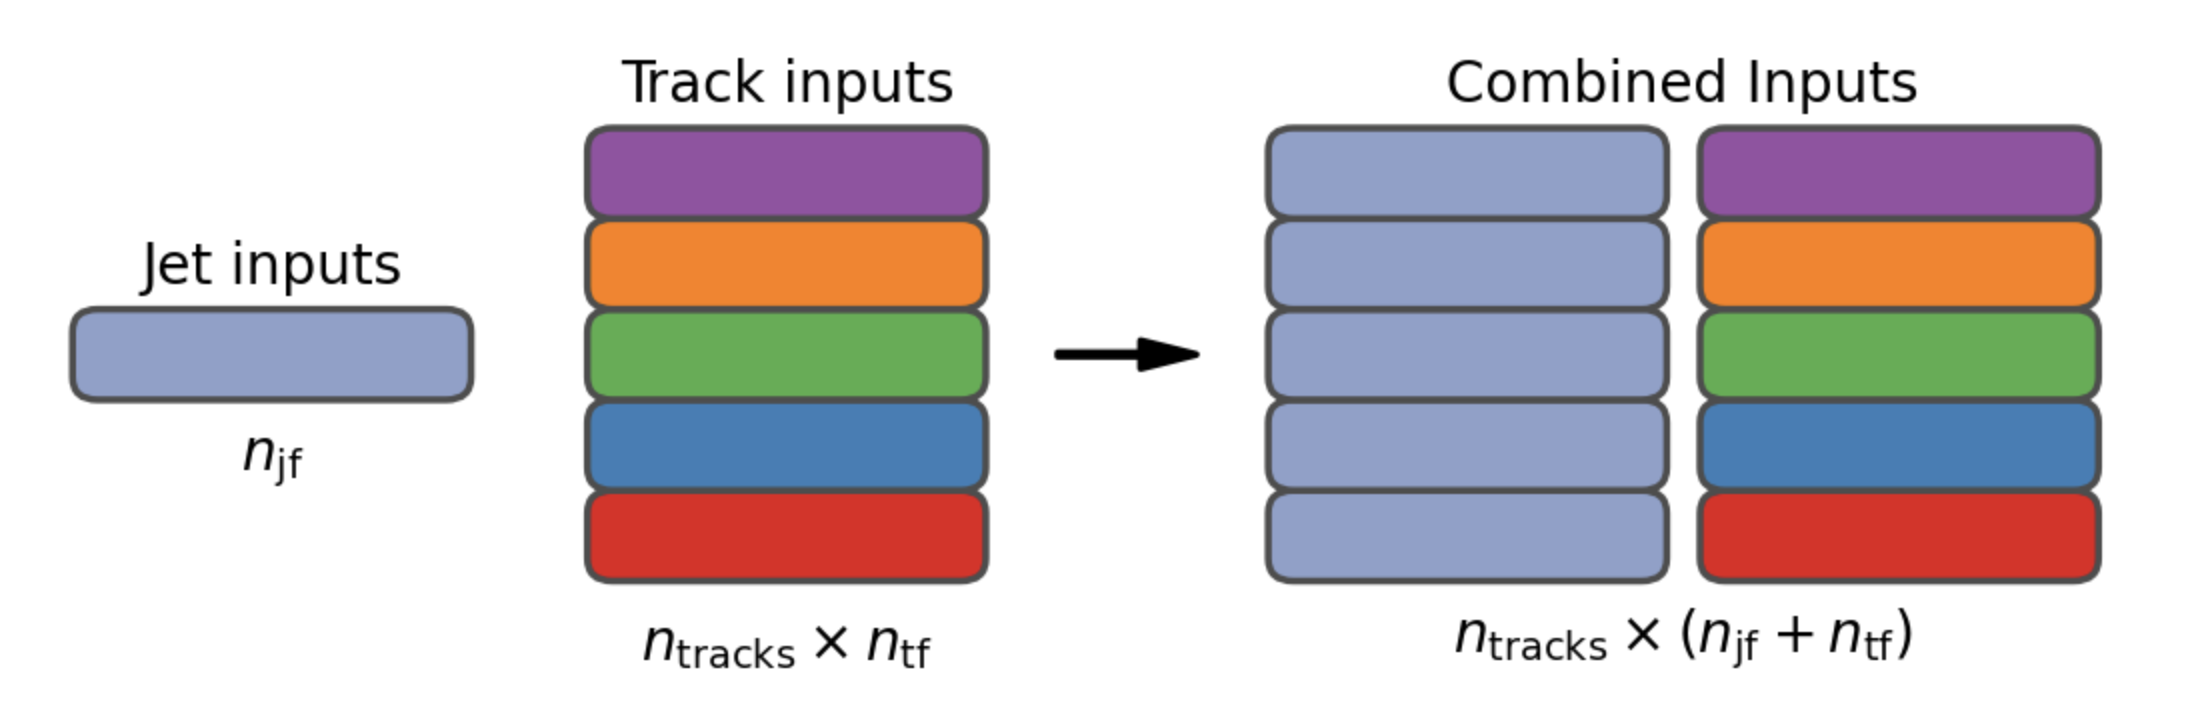
\includegraphics[width=0.6\textwidth]{chapters/gnn_tagger/figs/inputs_diagram.png}
    \caption{The inputs to \GNN are the two jet features ($n_\text{jf} = 2$), and an array of $n_{\text{tracks}}$, where each track is described by 21 track features ($n_\text{tf} = 21$). The jet features are copied for each of the tracks, and the combined jet-track vectors of length 23 form the inputs of \GNN.}
    \label{fig:model_input_array}
\end{figure}

\begin{figure}[!htbp]
    \centering
    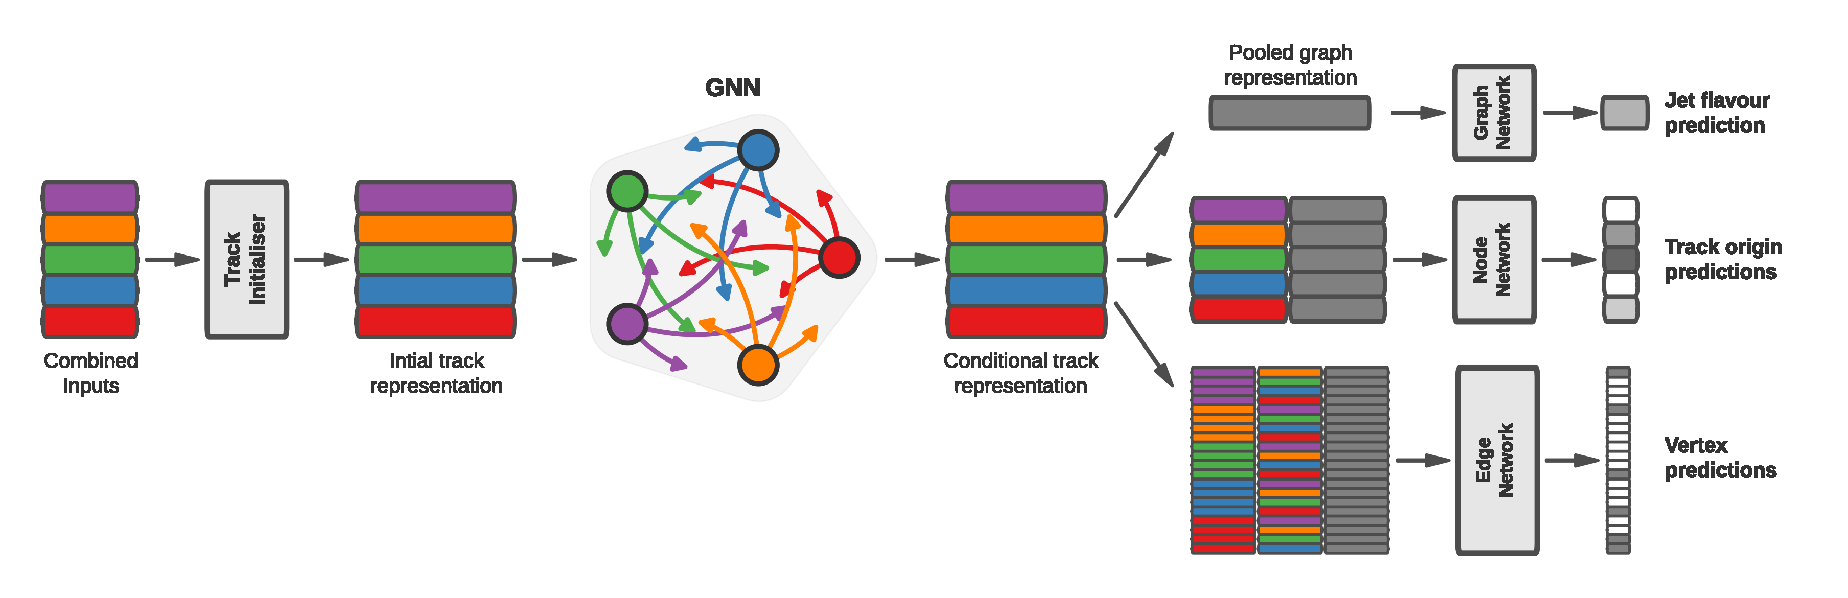
\includegraphics[width=\textwidth]{chapters/gnn_tagger/figs/full_arch.pdf}
    \caption{The network architecture of \GNN. Inputs are fed into a per-track initialisation network, which outputs an initial latent representation of each track. These representations are then used to populate the node features of a fully connected graph network. After the graph network, the resulting node representations are used to predict the jet flavour, the track origins, and the track-pair vertex compatibility.}
    \label{fig:new_arch}
\end{figure}


A fully connected graph is built from the outputs of the track initialisation network, such that each node in the graph neighbours every other node.
Each node $h_i$ in the graph corresponds to a single track in the jet, and is characterised by a feature vector, or representation.
The per-track output representations from the initialisation networks are used to populate the initial feature vectors of each node in the graph.
In each layer of the graph network, output node representations $h_i'$ are computed by aggregating the features of $h_i$ and neighbouring nodes $\mathcal{N}_i$ as described in Ref.~\cite{2021arXiv210514491B}.
First, the feature vectors of each node are fed into a fully connected layer $\mathbf{W}$, to produce an updated representation of each node $\mathbf{W} h_i$.
These updated feature vectors are used to compute edge scores $e(h_i, h_j)$ for each node pair,

\begin{equation}\label{eq:edge_score}
    e(h_i, h_j) = \mathbf{a}^\perp \theta \left[ \mathbf{W}h_i \oplus \mathbf{W}h_j \right],
\end{equation}

where $\oplus$ denotes vector concatenation, $\theta$ is a non-linear activation function, and $\mathbf{a}$ is a learned vector.
These edge scores are then used to calculate attention weights $a_{ij}$ for each pair of nodes using the softmax function over the edge scores

\begin{equation}\label{eq:attention weights}
    a_{ij} = \mathrm{softmax}_j \left[ e(h_i, h_j) \right].
\end{equation}

Finally, the updated node representation $h_i'$ is computed by taking the weighted sum over each updated node representation $\mathbf{W} h_i$, with weights $a_{ij}$

\begin{equation}\label{eq:updated_node_rep}
    h'_i = \sigma \left[ \sum_{j \in \mathcal{N}_i}{a_{ij} \cdot \mathbf{W} {h}_j}  \right].
\end{equation}

The above set of operations constitute a single graph network layer. 
Three such layers are stacked to construct the graph network, representing a balance between achieving optimal performance and preventing overtraining.
The final output node feature vectors from the network are representations of each track that are conditional on the other tracks in the jet.
The output representation for each track is combined using a weighted sum to construct a global representation of the jet, where the attention weights for the sum are learned during training.
Three separate fully connected feedforward neural networks are then used to independently perform the different classification objectives of \GNN.
Each of the objectives makes use of the global representation of the jet.
A summary of the different classification networks used for the various training objectives is shown in \cref{tab:architecture}.

\begin{table}[!htbp]
  \footnotesize\centering
  \setlength{\tabcolsep}{0.5em} % for the horizontal padding
  \caption{
      A summary of GN1's different classification networks used for the different training objectives.
      The hidden layers column contains a list specifying the number of neurons in each layer.
      }
  \begin{tabular}{lll}
      \toprule\hline 
      \textbf{Network} & \textbf{Hidden layers} & \textbf{Output size} \\
      \hline
      Node classification network    & 128, 64, 32 & 7 \\
      Edge classification network    & 128, 64, 32 & 1 \\
      Graph classification network   & 128, 64, 32, 16 & 3 \\
      \hline\bottomrule
  \end{tabular}
  \vspace{4mm}
  \label{tab:architecture}
\end{table}



A node classification network, which takes as inputs the features from a single output node from the graph network and the global jet representation, predicts the track truth origin, as defined in \cref{tab:truth_origins}.
This network has three hidden layers containing 128, 64 and 32 neurons respectively, and an output size of seven, corresponding to the seven different truth origins.

An edge classification network, which takes as inputs the concatenated representations from each pair of tracks and the global jet representation, is used to predict whether the tracks in the track-pair belong to a common vertex.
The edge network has three hidden layers containing 128, 64 and 32 neurons respectively, and a single output, which is used to perform binary classification of the track-pair compatability.
These predictions are used for the auxiliary training objectives discussed in \cref{sec:aux-train-objectives}.

A graph classification network takes only the global jet representation as an input, and predicts the jet flavour. 
The graph classification network is comprised of four fully connected hidden layers with 128, 64, 32 and 16 neurons respectively, and has three outputs corresponding to the \bcl jet classes. 



\subsection{Training}\label{sec:training}

The full \GNN training procedure minimises the total loss function $L_\text{total}$, defined in \cref{eq:loss}. 
This loss is composed of three terms: $L_\text{jet}$, the categorical cross entropy loss over the different jet flavours; $L_\text{vertex}$, the binary track-pair compatability cross entropy loss averaged over all track-pairs; and $L_\text{track}$, the categorical cross entropy loss for the track origin prediction. $L_\text{vertex}$ is computed by averaging over all track-pairs in the batch, and $L_\text{track}$ is computed by averaging over all tracks in the batch.

\begin{equation}\label{eq:loss}
    L_\text{total} = L_\text{jet} + \alpha L_\text{vertex} + \beta L_\text{track}
\end{equation}

The different losses converge to different values during training, reflective of differences in the relative difficulty of the various objectives.
As such, $L_\text{vertex}$ and $L_\text{track}$ are weighted by $\alpha = 1.5$ and $\beta = 0.5$ respectively to ensure they converge to similar values, giving them an equal weighting towards $L_\text{total}$. 
The values of $\alpha$ and $\beta$ also ensure that $L_\text{jet}$ converges to a larger value than $L_\text{vertex}$ and $L_\text{track}$, reflecting the primary importance of the jet classification objective.
In practice, the final performance of the model was not sensitive to modest variations in the loss weights $\alpha$ and $\beta$, or to pre-training using $L_\text{total}$ and fine tuning on the jet classification task only.
As there was a significant variation in the relative frequency of tracks of different origins, the contribution of each origin class to $L_\text{track}$ was weighted by the inverse of the frequency of their occurrence.
In $L_\text{vertex}$, the relative class weight in the loss for track-pairs where both tracks are from either a \borchadron is increased by a factor of two as compared with other track-pairs.

The track classification and vertexing objectives are supplementary to the jet classification objective and trainings can be performed with either the node or edge networks, or both, removed, as discussed in \cref{sec:gnn_ablations}.
In these cases, the corresponding losses $L_\text{vertex}$ and $L_\text{track}$ are removed from the calculation of $L_\text{total}$. 
The resulting trainings demonstrate how useful the different auxiliary training objectives are for the primary jet classification objective.

\GNN trainings are run for \nepochs epochs on 4 NVIDIA V100 GPUs, taking around \minsperepoch mins to complete each epoch over the training sample of \njetstrain jets described in \cref{sec:datasets}.
The Adam optimiser~\cite{arxiv.1412.6980} with an initial learning rate of $1\mathrm{e}{-3}$, and a batch size of 4000 jets (spread across the 4 GPUs) was used.
Typically the validation loss, calculated on \njetsval jets, stabilised after around 60 epochs.
The epoch that minimized the validation loss was used for evaluation.
\GNN has been integrated into the ATLAS software~\cite{ATL-SOFT-PUB-2021-001} using ONNX~\cite{bai2019}, and jet flavour predictions for the test sample are computed using the ATLAS software stack.
%\todo{inlcude loss vs epoch? or save for paper}


\section{Results}\label{sec:gnn_results}


The performance of the \GNN tagger is evaluated for both \btag and \ctag use cases, and for both jets with \ttbarpt from the \ttbar sample and jets with \Zprimept from the \Zprime sample.
Performance is compared to the \DLr tagger \cite{ATL-PHYS-PUB-2017-013}, which has been retrained on 75 million jets from the same samples as \GNN.
%Sample prepration is identical for the different models.
The input RNNIP tagger \cite{ATL-PHYS-PUB-2017-003} to \DLr has not been retrained.
%\DLr is a modification of the previous \DLr tagger \cite{ATL-PHYS-PUB-2017-013} which which replaces RNNIP with DIPS, a separately trained track-based algorithm based on deep sets. 
%The DIPS tagger uses the loose track selection defined in \cite{ATL-PHYS-PUB-2020-014}.

The taggers predict the probability that a jet belongs to the \bcl classes. To use the model for \btag, these probabilities are combined into a single score \Db, defined as

\begin{equation}\label{eq:btag-disc}
    \Db = \log{\frac{p_b}{(1-\fc )p_l + \fc  p_c}} ,
\end{equation}

where \fc is a free parameter that determines the relative weight of $p_c$ to $p_l$ in the score \Db, controlling the trade-off between $c$- and \lrej performance.
This parameter is set to a value of $\fc = 0.018$ for the \DLr model, obtained through an optimisation procedure designed to maximise the \clrej of \DLr \cite{ATL-PHYS-PUB-2017-013}.
For the \GNN models a value of $\fc = 0.05$ is used, based on a similar optimisation procedure.
The choice of \fc is arbitrary, with the different optimised values reflecting the relative $c$- versus light-jet rejection performance of the various taggers.
A fixed-cut working point (WP) defines the corresponding selection applied to the tagging discriminant \Db in order to achieve a given inclusive efficiency on the \ttbar sample.

The technical implementation of \GNN results in any jet with no associated tracks or exactly one associated track to be classified as a \ljet.
The impact of this on the tagging performance of \GNN was found to be negligible, with \pct{0.12} of \ttbarbjets and \pct{0.02} of \Zprimebjets affected.
Of those, \pct{89} of the \ttbarbjets and \pct{98} of the \Zprimebjets are classified as \ljets by \DLr at the \pct{70} \ttbar WP.

A comparison of the \btag discriminant \Db between \DLr and \GNN is given in \cref{fig:ttbar_btag_disc}. 
The shapes of the distributions are broadly similar for \bcl jets, however, the \GNN model shifts the \bjet distribution to higher values of \Db in the regions with the best discrimination.
The \GNN \cjet distribution is also shifted to lower values of \Db when compared with \DLr, enhancing the separation and indicating that \GNN will improve \cjet rejection when compared with \DLr.

\begin{figure}[!htb]
    \centering
    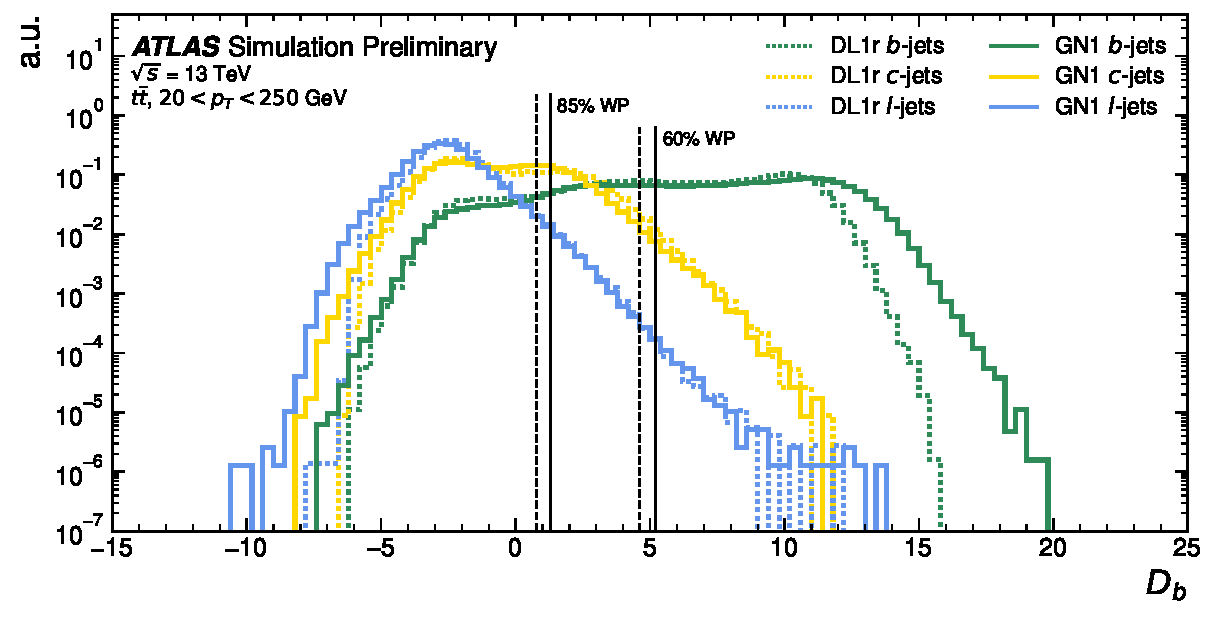
\includegraphics[width=0.6\textwidth]{chapters/gnn_tagger/figs/results/main/ttbar/ttbar_score_DL1r_GN120220509_btag.pdf}
    \caption{Comparison between the \DLr and \GNN \btag discriminant \Db for jets in the \ttbar sample.
    The \pct{85} WP and the \pct{60} WP are marked by the solid (dashed) lines for \GNN (\DLr), representing respectively the loosest and tightest WPs used by analyses.
    A value of $\fc = 0.018$ is used in the calculation of \Db for \DLr and $\fc = 0.05$ is used for \GNN. The distributions of the different jet flavours have been normalised to unity area.}
    \label{fig:ttbar_btag_disc}
\end{figure}



\subsection{\texorpdfstring{\btagging}{b-tagging} Performance}\label{sec:gnn_btag_perf}

The performance of a \btag algorithm is quantified by its power to reject \cljets for a given $b$-jet tagging efficiency, or WP. 
In order to compare the \btag performance of the different taggers for the $b$-jet tagging efficiencies in the range typically used by analyses, the corresponding \clrej rates are displayed in \cref{fig:ttbar_btag_roc,fig:zprime_btag_roc} for jets in the \ttbar and \Zprime samples respectively.
Four standard WPs with $b$-jet tagging efficiencies of \pct{60}, \pct{70}, \pct{77} and \pct{85} are used by physics analyses depending on their specific signal and background requirements.
These WPs are defined using \ttbarjets only.
The $b$-jet tagging efficiencies for \Zprimejets are lower than the corresponding WPs calculated in the \ttbar sample, due to the much higher jet \pt range in the \Zprime sample.
For instance the WP defined to provide a $70\%$ $b$-jet tagging efficiency on the \ttbar sample results in a $b$-jet tagging efficiency of $\sim30\%$ on the \Zprime sample.
To account for this, the range of $b$-jet tagging efficiencies displayed in \cref{fig:zprime_btag_roc} is chosen to span the lower values achieved in the \Zprime sample.

For \ttbarjets with \ttbarpt, \GNN demonstrates considerably better \clrej compared with \DLr across the full range of $b$-jet tagging efficiencies probed.
The relative improvement depends on the \bjet tagging efficiency, with the largest improvements found at lower values.
At a $b$-jet tagging efficiency of \pct{\ttlo}, the \crej improves by a factor of \ttbclo and the \lrej improves by a factor of \ttbllo with respect to \DLr.
For high-\pt \Zprimejets with \Zprimept, \GNN also brings considerable performance improvements with respect to \DLr across the range of $b$-jet tagging efficiencies studied.
Again, the largest relative improvement in performance comes at lower $b$-jet tagging efficiencies.
At a $b$-jet tagging efficiency of \pct{\zplo}, \GNN improves the \crej by a factor of \zpbclo and the \lrej by a factor of \zpbllo.
An increasing statistical uncertainty due to the high rejection of background affects the comparison at lower $b$-jet tagging efficiencies.
It is estimated that for a $b$-jet tagging efficiency of $70\%$ in the \ttbar sample, $\sim5\%$ ($\sim30\%$) of the relative improvement in the $c$-jet (light-jet) rejection comes from loosening the track selection and for a $b$-jet tagging efficiency of $30\%$ in the \Zprime the corresponding number is $\sim10\%$ for both $c$-jets and light-jets.
Given the sophisticated exploitation of low-level information, further studies are needed to confirm if the performance gain is also observed in experimental data.

The \GNNLep variant shows improved performance with respect to the baseline \GNN model, demonstrating the additional jet flavour discrimination power provided by the leptonID track input.
For \ttbarjets, the relative \crej improvement with respect to \DLr at the \bWP{\ttlo} increases from a factor of \ttbclo for \GNN to a factor of $\sim 2.8$ for \GNNLep.
The improvement in \lrej also increases from a factor of \ttbllo to $\sim 2.5$ at this WP.
For \Zprimejets, the relative \crej (\lrej) improvement with respect to \DLr increases from a factor of \zpbclo to $\sim 3$ (\zpbllo to $\sim 7.5$) at a $b$-jet tagging efficiency of \pct{\zplo}.
As shown in \cref{fig:vs_pt_flat_leff}, the greatest improvement of \GNNLep over \GNN is seen at low \pt.

\begin{figure}[!p]
    \centering
    \includegraphics[width=\textwidth]{chapters/gnn_tagger/figs/results/main/ttbar/ttbar_roc_btag.pdf}
    \caption{The \cjet (left) and \ljet (right) rejections as a function of the $b$-jet tagging efficiency for \ttbarjets with \ttbarpt.
             The ratio with respect to the performance of the \DLr algorithm is shown in the bottom panels.
             A value of $\fc = 0.018$ is used in the calculation of \Db for \DLr and $\fc = 0.05$ is used for \GNN and \GNNLep.
             Binomial error bands are denoted by the shaded regions.
             At \bjet tagging efficiencies less than $\sim$\pct{75}, the \lrej becomes so large that the effect of the low number of jets is visible.
             The lower $x$-axis range is chosen to display the \bjet tagging efficiencies usually probed in these regions of phase space.}
    \label{fig:ttbar_btag_roc}
\end{figure}

\begin{figure}[!p]
    \centering
    \includegraphics[width=\textwidth]{chapters/gnn_tagger/figs/results/main/zprime/zprime_roc_btag.pdf}
    \caption{The \cjet (left) and \ljet (right) rejections as a function of the $b$-jet tagging efficiency for \Zprimejets with \Zprimept.
             The ratio with respect to the performance of the \DLr algorithm is shown in the bottom panels.
             A value of $\fc = 0.018$ is used in the calculation of \Db for \DLr and $\fc = 0.05$ is used for \GNN and \GNNLep.
             Binomial error bands are denoted by the shaded regions.
             At \bjet tagging efficiencies less than $\sim$\pct{20}, the \lrej becomes so large that the effect of the low number of jets is visible.
             The lower $x$-axis range is chosen to display the \bjet tagging efficiencies usually probed in these regions of phase space.}
    \label{fig:zprime_btag_roc}
\end{figure}

The performance of the taggers is strongly dependent on the jet \pt.
Charged particle reconstruction is particularly challenging within high-\pt jets \cite{PERF-2015-08}.
The multiplicity of fragmentation particles increases as a function of \pt, while the number of particles from heavy flavour decays stays constant.
Collimation of particles inside the jet increases and approaches the granularity of the tracking detectors, making it difficult to resolve the trajectories of different particles.
Furthermore, at high \pt, heavy flavour hadrons will travel further into the detector before decaying.
For hadrons which traverse one or more layers of the ID before decaying, the corresponding decay tracks may pick up incorrect hits, left by the hadron itself or fragmentation particles, in the inner layers of the detector, reducing the accuracy of the reconstructed track parameters.
These factors contribute to a reduced reconstruction efficiency for heavy flavour tracks, and a general degradation in quality of tracks inside the core of a jet, which in turn reduces the jet classification performance.

% In order to study how the \bseleff of the taggers varies as a function of jet \pt, the \beff for \ttbarZprimejets at a fixed \pct{77} \ttbar WP is shown in as a function of \pt in \cref{fig:vs_pt_fixed_ttbar}.
% For \ttbarjets, the different taggers perform similarly in the different \pt bins.
% Performance for jets with $\pt < \SI{100}{\GeV}$ is lower than jets with $\pt > \SI{100}{\GeV}$ due to the shorter flight distance of the \bhadron in low \pt jets.
% For \Zprimejets at the \pct{77} \ttbar WP, the efficiency for each of the taggers starts high at around \pctr{60}{70} for $\pt < \SI{1}{\TeV}$, and then drops with increasing \pt, beginning to plateau at around \pctr{5}{15} above \SI{4}{\TeV}.
% At low $\pt < \SI{500}{\GeV}$, the \beff at a fixed \leff for \DLr (\GNN) is \pct{65} (\pct{75}), and this drops to approximately \pct{10} (\pct{20}) as the jet \pt moves to extreme ranges of up to $\pt > \SI{4}{\TeV}$.
% At \SI{1}{\TeV}, \GNN improves the \beff at a fixed \ceff (\leff) as compared with \DLr by \pct{10} (\pct{20}).
% Above \SI{4}{\TeV}, the relative increase in \bjet tagging efficiency between \DLr and \GNN is larger, with increases of up to \pct{30} (\pct{80}) at a fixed \crej (\lrej).

% The \bseleff of the \GNNLep variant is similar to the baseline \GNN model for both \ttbarZprimejets at the \pct{77} \ttbar WP.
In order to study how the $b$-jet tagging efficiency of the taggers varies as a function of jet \pt, the $b$-jet tagging efficiency as a function of \pt for a fixed light-jet rejection of 100 in each bin is shown in \cref{fig:vs_pt_flat_leff}.
For \ttbarjets, at a fixed \ljet rejection of 100, \GNN improves the $b$-jet tagging efficiency by approximately \pct{4} across all jet \pt bins.
\GNNLep shows improved performance with respect to \GNN, in particular at lower \pt, with the relative increase in the $b$-jet tagging efficiency going from \pct{4} to \pct{8}.
For \Zprimejets, \GNN has a higher $b$-jet tagging efficiency than \DLr across the \pt range, with the largest relative improvement in performance, approximately a factor of 2, found at jet $\pt > \SI{2}{\TeV}$.
\GNN outperforms \DLr across the entire jet \pt spectrum studied. 
The performance was also evaluated as a function of the average number of pileup interactions in an event, and was found to have no significant dependence on this quantity.

% \begin{figure}[!p]
%     \centering
%     \begin{subfigure}[b]{0.48\textwidth}
%         \centering
%         \includegraphics[width=\textwidth]{chapters/gnn_tagger/figs/results/main/ttbar/ttbar_fixed_beff_by_pt_btag.pdf}
%         %\caption{sub}
%         %\label{fig:sub}
%     \end{subfigure}
%     \quad
%     \begin{subfigure}[b]{0.48\textwidth}
%         \centering
%         \includegraphics[width=\textwidth]{chapters/gnn_tagger/figs/results/main/zprime/zprime_fixed_beff_by_pt_btag.pdf}
%         %\caption{sub}
%         %\label{fig:sub}
%     \end{subfigure}
%     \caption{The \btag efficiency for \ttbarjets (left) and \Zprime jets (right) as a function of jet \pt for a fixed \pct{77} \ttbar \beff.
%              For \ttbarjets, the taggers show a similar response in the different \pt bins.
%              For \Zprimejets, performance drops off with increasing \pt for all taggers, though \GNN improves the \beff by up to a factor of 2.5 for jets with $\pt > \SI{3}{\TeV}$.
%              The standard error on the mean is shown in the shaded regions.
%              }
%     \label{fig:vs_pt_fixed_ttbar}
% \end{figure}


\begin{figure}[!htbp]
    \centering
    \begin{subfigure}[b]{0.48\textwidth}
        \centering
        \includegraphics[width=\textwidth]{chapters/gnn_tagger/figs/results/main/ttbar/ttbar_flat_leff_by_pt_btag.pdf}
        %\caption{sub}
        %\label{fig:sub}
    \end{subfigure}
    \quad
    \begin{subfigure}[b]{0.48\textwidth}
        \centering
        \includegraphics[width=\textwidth]{chapters/gnn_tagger/figs/results/main/zprime/zprime_flat_leff_by_pt_btag.pdf}
        %\caption{sub}
        %\label{fig:sub}
    \end{subfigure}
    \caption{The \bjet tagging efficiency for \ttbarjets (left) and \Zprimejets (right) as a function of jet \pt with a fixed \ljet rejection of 100 in each bin.
             %For \ttbarjets, \GNN increases \beff by approximately \pct{5} with respect to \DLr in each \pt bin.
             %For \Zprimejets, \GNN increases \beff by up to a factor of 2 for jets with $\pt > \SI{2.5}{\TeV}$ with respect to \DLr.
             A value of $\fc = 0.018$ is used in the calculation of \Db for \DLr and $\fc = 0.05$ is used for \GNN and \GNNLep.
             %\GNN demonstrates improved performance with respect to \DLr accross the \pt range.
             Binomial error bands are denoted by the shaded regions.
             }
    \label{fig:vs_pt_flat_leff}
\end{figure}




\subsection{\texorpdfstring{\ctagging}{c-tagging} Performance}\label{sec:gnn_ctag_perf}

Since \GNN does not rely on any manually optimised low-level tagging algorithms, which may not have been optimised for \ctag, tagging \cjets presents a compelling use case for \GNN.
To use the model for \ctag, the output probabilities are combined into a single score \Dc, defined similarly to \cref{eq:btag-disc} as

\begin{equation}\label{eq:ctag-disc}
    D_c = \log{\frac{p_c}{(1-f_b)p_l + f_b p_b}} .
\end{equation}

A value of $\fb = 0.2$ is used for all models.
Similar to \cref{sec:gnn_btag_perf}, performance of the different taggers is compared by scanning through a range of $c$-jet tagging efficiencies and plotting the corresponding \blrej rates.
As in \cref{sec:gnn_btag_perf}, WPs are defined using \ttbarjets.
Standard $c$-jet tagging efficiency WPs are significantly lower in comparison with the \btag WPs in order to maintain reasonable $b$- and light-jet rejection rates.
This is reflected in the range of $c$-jet tagging efficiencies used in \cref{fig:ttbar_ctag_roc,fig:zprime_ctag_roc}.
In \cref{fig:ttbar_ctag_roc}, which displays the \ctag performance of the models on the \ttbarjets, \GNN performs significantly better than \DLr.
The \blrej improve most at lower $c$-jet tagging efficiencies, with both background rejections increasing by a factor of 2 with respect to \DLr at a $c$-jet tagging efficiency of \pct{25}.
\GNNLep outperforms \GNN, with the \brej (\lrej) relative improvement increasing from a factor of 2 to 2.1 (2 to 2.3) at the \WP{25}{c}.
\cref{fig:zprime_ctag_roc} shows the \ctag performance on the \Zprimejets.
Both \GNN and \GNNLep perform similarly, improving the \brej by \pct{60} and the \lrej by a factor of 2 at the \WP{25}{c}.

\begin{figure}[!p]
    \centering
    \includegraphics[width=\textwidth]{chapters/gnn_tagger/figs/results/main/ttbar/ttbar_roc_ctag.pdf}
    \caption{
        The \bjet (left) and \ljet (right) rejections as a function of the $c$-jet tagging efficiency for \ttbar jets with \ttbarpt.
        The ratio to the performance of the \DLr algorithm is shown in the bottom panels.
        Binomial error bands are denoted by the shaded regions.
        At $c$-jet tagging efficiencies than $\sim$\pct{25}, the \lrej becomes so large that the effect of the low number of jets is visible.
        The lower $x$-axis range is chosen to display the \cjet tagging efficiencies usually probed in these regions of phase space.
    }
    \label{fig:ttbar_ctag_roc}
\end{figure}

\begin{figure}[!p]
   \centering
   \includegraphics[width=\textwidth]{chapters/gnn_tagger/figs/results/main/zprime/zprime_roc_ctag.pdf}
   \caption{
        The \bjet (left) and \ljet (right) rejections as a function of the $c$-jet tagging efficiency for \Zprime jets with \Zprimept.
        The ratio to the performance of the \DLr algorithm is shown in the bottom panels.
        Binomial error bands are denoted by the shaded regions.
        The lower $x$-axis range is chosen to display the \cjet tagging efficiencies usually probed in these regions of phase space.
    }
   \label{fig:zprime_ctag_roc}
\end{figure}



\subsection{Jet Display Diagrams}

\begin{figure}[!p]
    \centering
    \includegraphics[width=0.95\textwidth]{chapters/gnn_tagger/figs/bjet_vertex.pdf}
    \caption{
        A schematic showing the truth track origin and vertex information (left) compared with the predictions from \GNN (right).
        Vertices reconstructed by SV1 and JetFitter are also marked.
    }
    \label{fig:bjet_diag_1}
 \end{figure}


 \begin{figure}[!p]
    \centering
    \includegraphics[width=0.95\textwidth]{chapters/gnn_tagger/figs/bjet_vertex2.pdf}
    \caption{
        A schematic showing the truth track origin and vertex information (left) compared with the predictions from \GNN (right).
        Vertices reconstructed by SV1 and JetFitter are also marked.
    }
    \label{fig:bjet_diag_2}
 \end{figure}

 

\subsection{Ablations}\label{sec:gnn_ablations}

Several ablations, the removal of components in the model to study their impact, are carried out to determine the importance of the auxiliary training objectives of \GNN to the overall performance.
The ``\GNN No Aux'' variant retains the primary jet classification objective, but removes both track classification and vertexing auxiliary objectives (see \cref{sec:aux-train-objectives}) and as such only minimises the jet classification loss.
The ``\GNN TC'' variant includes track classification but not vertexing, while ``\GNN Vert'' includes vertexing, but not track classification.

For jets in both the \ttbar and \Zprime samples, the models without one or both of the auxiliary objectives display significantly reduced \clrej when compared with the baseline \GNN model, as shown in \cref{fig:ttbar_btag_roc_ab,fig:zprime_btag_roc_ab}.
For \ttbarjets, the performance of \GNN No Aux is similar to \DLr, while \GNN TC and \GNN Vert perform similarly to each other.
% with improvements in the \crej of \pct{80} and improvements in the \lrej of \pct{75} at a $b$-jet tagging efficiency of \pct{60}.
For \Zprimejets, the \GNN No Aux model shows a clear improvement in \clrej when compared with \DLr at lower $b$-jet tagging efficiencies.
Similar to \ttbarjets, \GNN TC and \GNN Vert perform similarly, and bring large gains in background rejection when compared with \GNN No Aux, but the combination of both auxiliary objectives yields the best performance.

It is notable that the \GNN No Aux model matches or exceeds the performance of \DLr without the need for inputs from the low-level algorithms.
This indicates that the performance improvements enabled by \GNN appear to be able to compensate for the removal of the low-level algorithm inputs.
The \GNN TC and \GNN Vert variants each similarly outperform \DLr, demonstrating that both contribute to the overall high performance of the baseline model.


\begin{figure}[!p]
    \centering
    \includegraphics[width=\textwidth]{chapters/gnn_tagger/figs/results/ablations/ttbar/ttbar_roc_btag.pdf}
    \caption{The \cjet (left) and \ljet (right) rejections as a function of the \bjet tagging efficiency for \ttbar jets with \ttbarpt, for the nominal \GNN, in addition to configurations where no (\GNN No Aux), only the track classification (\GNN TC) or only the vertexing (\GNN Vert) auxiliary objectives are deployed. The ratio to the performance of the \DLr algorithm is shown in the bottom panels. A value of $\fc = 0.018$ is used in the calculation of \Db for \DLr and $\fc = 0.05$ is used for \GNN. Binomial error bands are denoted by the shaded regions. At \bjet tagging efficiencies less than $\sim65\%$, the \lrej become so large that the effect of the low number of jets are visible. The lower $x$-axis range is chosen to display the \bjet tagging efficiencies usually probed in these regions.}
    \label{fig:ttbar_btag_roc_ab}
\end{figure}

\begin{figure}[!p]
    \centering
    \includegraphics[width=\textwidth]{chapters/gnn_tagger/figs/results/ablations/zprime/zprime_roc_btag.pdf}
    \caption{The \cjet (left) and \ljet (right) rejections as a function of the \bjet tagging efficiency for \Zprime jets with \Zprimept, for the nominal \GNN, in addition to configurations where no (\GNN No Aux), only the track classification (\GNN TC) or only the vertexing (\GNN Vert) auxiliary objectives are deployed. The ratio to the performance of the \DLr algorithm is shown in the bottom panels. A value of $\fc = 0.018$ is used in the calculation of \Db for \DLr and $\fc = 0.05$ is used for \GNN. Binomial error bands are denoted by the shaded regions. At \bjet tagging efficiencies less than $\sim25\%$, the \lrej become so large that the effect of the low number of jets are visible. The lower $x$-axis range is chosen to display the \bjet tagging efficiencies usually probed in these regions.}
    \label{fig:zprime_btag_roc_ab}
\end{figure}



\subsection{Inclusion of Low-Level Vertexing Algorithms}\label{sec:gnn_low_level_vert_impact}

\GNN does not include inputs from low-level tagging algorithms, including the vertexing tools SV1 and JetFitter \cite{FTAG-2018-01}.
Since these algorithms are known to improve the performance of \DLr, it was feasible that their inclusion in \GNN may further improve on the performance of the \GNN models.
In a dedicated training of \GNN the SV1 and JetFitter tagger outputs were added to the \GNN jet classification network as an input, similar to their use in \DLr.
These outputs include information on the reconstructed vertices, including the number of vertices, the vertex mass, displacement, and other properties.
In addition, the index of the reconstructed SV1 or JetFitter vertices were included as two track-level inputs to \GNN. 
%These indices were also used to construct an edge feature for the edge classification network, which was given a value of one if the track-pair were from a common reconstructed V1 or JetFitter vertex, and zero otherwise.
The jet classification performance of this \GNN model was not significantly different to the baseline model, and in some cases the performance was slightly reduced.
%As \GNN does not benefit from the inclusion of information from SV1 and JetFitter it can function as a highly performant standalone tagger that does not require (beyond etraining) any manual optimisation to achieve good performance in a wide range of phase spaces.
A dedicated look at the vertexing performance of \GNN with some comparisons to SV1 and JetFitter is found in \cref{sec:gnn_vert_perf}







\subsection{Vertexing Performance}\label{sec:gnn_vert_perf}

From the track-pair vertex prediction described in \cref{sec:aux-train-objectives}, tracks can be partitioned into compatible groups representing vertices (see \cite{serviansky2020set2graph}).
As such, \GNN is able to be used to perform vertex ``finding'', but not vertex ``fitting'', i.e. the reconstruction of a vertex's properties, which currently still requires the use of a dedicated vertex fitter.
In order to study the performance of the different vertexing tools inside \bjets, the truth vertex label of the tracks, discussed in \cref{sec:aux-train-objectives}, are used.
To estimate the efficiency with which \GNN manages to find vertices inclusively, vertices from \GNN containing tracks identified as coming from a \bhadron are merged together and compared to the inclusive truth decay vertices that result from a \bhadron decay (where if there are multiple distinct truth vertices from a \bhadron decay they are also merged together).
Vertices are compared with the target truth vertex and the number of correctly and incorrectly assigned tracks is computed.
Since secondary vertex information is only recovered for reconstructed tracks, an efficiency of $100\%$ here denotes that all possible secondary vertices are recovered given the limited track reconstruction efficiency.
A vertex is considered matched if it contains at least $65\%$ of the tracks in the corresponding truth vertex, and has a purity of at least $50\%$.
\GNN manages to achieve an inclusive reconstruction efficiency in \bjets of $\sim80\%$, demonstrating that it effectively manages to identify the displaced vertices from \bhadron decays.

\subsubsection{More detail}

In order to study the performance of the different vertexing tools inside \bjets, the truth vertex label of the tracks, discussed in \cref{sec:aux-train-objectives}, is used.
The reconstructed vertices from \GNN, SV1 and JetFitter are compared to the target truth vertices in order to calculate the efficiencies of the different vertexing tools.
Since secondary vertex information is only recovered for reconstructed tracks, an efficiency of $100\%$ here denotes that all possible secondary vertices are recovered given the limited track reconstruction efficiency.

There are several caveats to a comparison of the vertexing tools which are a result of the different approaches they take to vertexing.
SV1 and JetFitter are designed to only find secondary vertices in the jet, whereas \GNN is also trained to determine which tracks in the jet belong to the primary vertex (the vertex of the hard scatter $pp$ interaction).
To account for this the \GNN vertex with the largest number of predicted primary tracks is excluded from the vertex finding efficiency calculation.
While JetFitter and \GNN aim to resolve each displaced vertex inside the jet, such that secondary vertices from \bhadron decays are found separately to tertiary vertices from $b \rightarrow c$ decay chains, SV1 by design attempts to find a single inclusive vertex per jet.
This inclusive vertex groups inclusive \bhadron decays.
These are tracks from the \bhadron decay itself (FromB) and tracks from $b \rightarrow c$ decays (FromBC).
In order to fairly compare the performance if the different tools, both the exclusive and inclusive vertex finding efficiency is studied.
For the exclusive vertex finding case JetFitter and \GNN can be directly compared, while a comparison with SV1 is not possible due to aforementioned design constraints.
The inclusive vertex finding performance of all three tools can be compared using the procedure outlined below.

The starting point for the secondary vertex finding efficiency in both the exclusive and inclusive cases is to select truth secondary vertices are those containing only inclusive \bhadron decays to be considered as initial targets.
For exclusive vertex finding, these truth secondary vertices can be used directly as the demoninator for the efficiency calculation.
Meanwhile for the inclusive efficiency all such truth secondary vertices in the jet are merged into a single inclusive target vertex.
Correspondingly, for the inclusive vertex finding case, the vertices found by JetFitter are merged into a single vertex, and the vertices found by \GNN with at least one predicted inclusive \bhadron decay track are also merged similarly.
SV1 does not require any vertex merging.

Next, in both cases for each truth secondary vertex, vertices in the jet found by the different vertexing tools are compared with the target truth vertex.
The number of correctly and incorrectly assigned tracks is computed.
In order to call a vertex efficient, it is required to contain at least $65\%$ of the tracks in the corresponding truth vertex, and to have a purity of at least $50\%$.
Single track vertices are required to have a purity of $100\%$.
Additionally, for \GNN only, at least one track in the vertex is required to have a predicted heavy flavour origin.


\begin{figure}[!htbp]
    \centering
    \begin{subfigure}[b]{0.48\textwidth}
        \centering
        \includegraphics[width=\textwidth]{chapters/gnn_tagger/figs/results/tracks/ttbar/ttbar_bjet_vert_eff_1+_track_excl.pdf}
        %\caption{sub}
        %\label{fig:sub}
    \end{subfigure}
    \quad
    \begin{subfigure}[b]{0.48\textwidth}
        \centering
        \includegraphics[width=\textwidth]{chapters/gnn_tagger/figs/results/tracks/ttbar/ttbar_bjet_vert_eff_2+_track_incl.pdf}
        %\caption{sub}
        %\label{fig:sub}
    \end{subfigure}
    \caption{Vertex finding efficiency as a function of jet \pt for \ttbarbjets using the exclusive (left) and inclusive (right) vertex finding approaches.
             Efficient vertex finding requires the recall of at least $65\%$ of the tracks in the truth vertex, and allows no more than $50\%$ of the tacks to be included incorrectly.
             Binomial error bands are denoted by the shaded regions.}
    \label{fig:ttbar_vert_eff}
\end{figure}

Vertex finding efficiencies for \ttbarbjets are displayed as a function of \pt separately for the inclusive and exclusive approaches in \cref{fig:ttbar_vert_eff}.
For \ttbarbjets with \ttbarpt, the exclusive vertex finding efficiency of JetFitter and \GNN is relatively flat as a function of \pt.
Of the truth secondary vertices in this \pt region, JetFitter efficiently finds approximately \pct{40} and \GNN finds approimately \pct{55}.
When finding vertices inclusively the vertex finding efficiency is generally higher.
An increased dependence on \pt is also visible for JetFitter and SV1. As the jet \pt increases from \SI{20}{\GeV} to \SI{100}{\GeV}, the efficiency of JetFitter increases from \pct{55} to \pct{65}.
In the same range, the efficiency of SV1 increases from \pct{55} to \pct{75}.
\GNN displays less dependence on \pt than JetFitter and SV1, efficiently finding upwards of \pct{80} of vertices in \bjets in this \pt region. 
For \bjets with $\pt > \SI{100}{\GeV}$, JetFitter finds approximately \pct{65} of vertices, SV1 finds approimately \pct{75} of vertices, and \GNN finds approximately \pct{80} of vertices.

For \Zprimebjets, the vertex finding efficiency drops steeply with increasing \pt up until $\pt = \SI{3}{\TeV}$.
\GNN outperforms SV1 and JetFitter across the \pt spectrum.
In the first bin, the efficiency of \GNN is $75\%$, while the efficiencies of SV1 and JetFitter are around $60\%$.
The efficiency of SV1 drops rapidly to almost zero above \SI{3}{\TeV}, while JetFitter and \GNN retain approximately $30\%$ efficiency.
\cref{fig:zprime_vert_eff} compares the exclusive vertex finding efficiencies of JetFitter and \GNN for multitrack vertices.
JetFitter finds $45\text{\nobreakdash-}50\%$ of vertices in \ttbarbjets, while \GNN finds $60\text{\nobreakdash-}65\%$.
For \Zprimebjets, JetFitter finds $35\%$ of vertices in the first bin, dropping to $20\%$ of vertices above \SI{2}{\TeV}.
\GNN finds $55\%$ of vertices in the first bin, dropping to $30\%$ above \SI{2}{\TeV}.


\begin{figure}[!htbp]
    \centering
    \begin{subfigure}[b]{0.48\textwidth}
        \centering
        \includegraphics[width=\textwidth]{chapters/gnn_tagger/figs/results/tracks/zprime/zprime_bjet_vert_eff_1+_track_excl.pdf}
        %\caption{sub}
        %\label{fig:sub}
    \end{subfigure}
    \quad
    \begin{subfigure}[b]{0.48\textwidth}
        \centering
        \includegraphics[width=\textwidth]{chapters/gnn_tagger/figs/results/tracks/zprime/zprime_bjet_vert_eff_2+_track_incl.pdf}
        %\caption{sub}
        %\label{fig:sub}
    \end{subfigure}
    \caption{Inclusive vertex finding efficiency for multitrack truth vertices in \ttbarbjets (left) and \Zprimejets (right) as a function of jet \pt. Efficient vertex finding requires the recall of at least $65\%$ of the tracks in the truth vertex, and allows no more than $50\%$ of the tacks to be included incorrectly.}
    \label{fig:zprime_vert_eff}
\end{figure}


%\GNN also outperforms JetFitter in single track exclusive vertex finding as shown in \cref{fig:vert_eff_1track_excl}, except at $\pt > 3 ~\TeV$, where the efficiency of JetFitter starts to increase.
%As shown in \cref{fig:vert_eff_1track_excl}, JetFitter has a high rate to find vertices in \ljets in this region of phase space.
%\cref{fig:vert_eff_1track_excl} shows the rate at which the different tools find vertices within \ljets as a function of jet \pt. 
%Found vertices in \ljets can correspond to real displaced truth vertices caused by for example material interactions, or can be comprised of tracks which do not originate from a common displaced truth vertex (``fake'' vertices).
%The SV1 rate remains low at under $10\%$ for \ttbarZprimeljets.
%
%\begin{figure}[!htbp]
%    \centering
%    \begin{subfigure}[b]{0.48\textwidth}
%        \centering
%        \includegraphics[width=\textwidth]{fig/results/tracks/ttbar/ttbar_vert_eff_1_track_excl.pdf}
%        %\caption{sub}
%        %\label{fig:sub}
%    \end{subfigure}
%    \quad
%    \begin{subfigure}[b]{0.48\textwidth}
%        \centering
%        \includegraphics[width=\textwidth]{fig/results/tracks/zprime/zprime_vert_eff_1_track_excl.pdf}
%        %\caption{sub}
%        %\label{fig:sub}
%    \end{subfigure}
%    \caption{Exclusive vertex finding efficiency for single track truth vertices in \ttbarbjets (left) and \Zprimejets (right) as a function of jet \pt. Efficient vertex finding in single track vertices requires the truth and found vertex to match exactly.}
%    \label{fig:vert_eff_1track_excl}
%\end{figure}
%
%For \ttbarljets, the rate of found JetFitter (\GNN) vertices increases as a function of \pt from 0.3 to 0.7 (0.5 to 1.1) vertices per jet.
%For \Zprimeljets, the vertexing rate of JetFitter plateaus above $3 ~\TeV$ at 2 vertices per jet, while the \GNN rate decreases steadily from 1.4 vertices for $\pt < 1 ~\TeV$ to 0.8 vertices above $4 ~\TeV$.
%By requiring that vertices found by \GNN also include at least one track with a predicted heavy flavour origin, as was done for the vertexing efficiency, the rate of \GNN vertices in \ljets can be suppressed to levels similar as found by SV1.
%Overall these results indicate that the \GNN model is able to efficiency find vertices when compared with SV1 and JetFitter.
%
%\begin{figure}[!htbp]
%    \centering
%    \begin{subfigure}[b]{0.48\textwidth}
%        \centering
%        \includegraphics[width=\textwidth]{fig/results/tracks/ttbar/ttbar_vert_fake_all_v2.pdf}
%        %\caption{sub}
%        %\label{fig:sub}
%    \end{subfigure}
%    \quad
%    \begin{subfigure}[b]{0.48\textwidth}
%        \centering
%        \includegraphics[width=\textwidth]{fig/results/tracks/zprime/zprime_vert_fake_all_v2.pdf}
%        %\caption{sub}
%        %\label{fig:sub}
%    \end{subfigure}
%    \caption{Vertex finding rate in \ljets for truth vertices in \ttbarbjets (left) and \Zprimejets (right) as a function of jet \pt. Found vertices in \ljets can correspond to real displaced vertices from secondary interactions or can be fake vertices. \GNN has a relatively high rate to find vertices in \ljets, though this can be suppressed by requiring that at least one track in the vertex have a predicted heavy flavour origin.}
%    \label{fig:vert_fake_all}
%\end{figure}



\subsection{Track Classification Performance}\label{sec:gnn_tc_perf}

As discussed in \cref{sec:aux-train-objectives}, one of the auxiliary training objectives for \GNN is to predict the truth origin of each track in the jet.
Since the equivalent information is not provided by any of the existing flavour tagging tools, as a benchmark a multi-class classification multilayer perceptron (MLP) is trained on the same tracks used for the baseline \GNN training.
The model uses the same concatenated track-and-jet inputs as \GNN (see \cref{sec:model-inputs}), but processes only a single track at a time.
The model is comprised of five densely connected layers with 200 neurons per layer, though the performance was not found to be strongly sensitive to changes in the network structure. 
To measure the track classification performance, the area under the curve (AUC) of the receiver operating characteristic (ROC) curve is computed for each origin class using a one versus all classification approach.
The AUCs for the different truth origin classes are averaged using both an unweighted and a weighted approach.
%Several metrics are used to measure the performance of the two models in \cref{tab:track_classification_metrics}, where the performance for the different truth origin classes is averaged over using both an unweighted and a weighted approach.
The unweighted mean treats the performance of each class equally, while the weighted mean uses the fraction of tracks from each origin as a weight.
As seen in \cref{tab:track_classification_metrics}, \GNN outperforms the MLP, both at \ttbarpt for \ttbarjets, and at \Zprimept for \Zprimejets.
For tracks in \ttbarjets, \GNN can reject \pct{65} of fake tracks while retaining more than \pct{99} of good tracks.
The \GNN model has two advantages over the MLP which can explain the performance improvement.
Firstly, the mixing of information between tracks, enabled by the fully connected graph network architecture as discussed in \cref{sec:Architecture}, is likely to be beneficial since the origins of different tracks within a jet are to some extent correlated.
Secondly, the jet classification and vertexing objectives can be considered auxiliary to the track classification task, and may bring improved track classification performance with respect to the standalone MLP.

\begin{table}[!htbp]
  \footnotesize\centering
  \setlength{\tabcolsep}{0.5em} % for the horizontal padding
  \begin{tabular}{cccccccccc}
      \toprule\hline 
      \multicolumn{1}{l}{}    & \multicolumn{1}{l}{} & \multicolumn{2}{c}{AUC}\\                               & \multicolumn{2}{c}{Precision}                           & \multicolumn{2}{c}{Recall}                              & \multicolumn{2}{c}{F1}                                  \\
      \multicolumn{1}{l}{}    & \multicolumn{1}{l}{} & \multicolumn{1}{c}{Mean} & \multicolumn{1}{c}{Weighted}\\ & \multicolumn{1}{c}{Mean} & \multicolumn{1}{c}{Weighted} & \multicolumn{1}{c}{Mean} & \multicolumn{1}{c}{Weighted} & \multicolumn{1}{c}{Mean} & \multicolumn{1}{c}{Weighted} \\
      \cmidrule(lr){3-4} \cmidrule(lr){5-6} \cmidrule(lr){7-8} \cmidrule(lr){9-10}

      \multirow{2}{*}{\ttbar} & 
      MLP & 0.87 & 0.89 \\ & & 0.39 & 0.71 & 0.51 & 0.56 & 0.36 & 0.62 \\ & 
      GN1 & \textbf{0.92} & \textbf{0.95} \\ & \textbf{0.51} & \textbf{0.82} & \textbf{0.64} & \textbf{0.70} & \textbf{0.51} & \textbf{0.74} 
      \\
      \multirow{2}{*}{\Zprime} & 
      MLP & 0.90 & 0.94 \\ & & 0.36 & 0.84 & 0.47 & 0.72 & 0.31 & 0.76 \\ &
      GN1 & \textbf{0.94} & \textbf{0.96} \\ & \textbf{0.48} & \textbf{0.88} & \textbf{0.60} & \textbf{0.79} & \textbf{0.48} & \textbf{0.82} \\             
      \hline\bottomrule
  \end{tabular}
  \caption{
    The area under the ROC curves (AUC) for the track classification from \GNN, compared to a standard multilayer perceptron (MLP) trained on a per-track basis. 
    The unweighted mean AUC over the origin classes and weighted mean AUC (using as a weight the fraction of tracks from the given origin) is provided.
    \GNN, which uses an architecture that allows track origins to be classified in a conditional manner as discussed in \cref{sec:Architecture}, outperforms the MLP model for both \ttbar and \Zprime jets.
  }
  \label{tab:track_classification_metrics}
\end{table}


\cref{fig:track_origin_roc} shows the track origin classification ROC curves for the different track origins for \ttbarZprimejets.
In order to improve legibility of the figure, the heavy flavour truth origins have been combined weighted by their relative abundance, as have the Primary and OtherSecondary labels.
In \ttbarZprimejets, the AUC of the different (grouped) origins is above $0.9$, representing good classification performance.
Fake tracks, followed by pileup tracks, are the easiest to classify in both samples.
%the FromC tracks which are \chadron decay products, are the hardest to classify, possibly due to their similarity to both fragmentation tracks and \bhadron decay tracks, depending on the \chadron in question.

\begin{figure}[!htbp]
    \centering
    \begin{subfigure}[b]{0.48\textwidth}
        \centering
        \includegraphics[width=\textwidth]{chapters/gnn_tagger/figs/results/tracks/ttbar/ttbar_origin_roc_GNNv11.pdf}
        %\caption{sub}
        %\label{fig:sub}
    \end{subfigure}
    \quad
    \begin{subfigure}[b]{0.48\textwidth}
        \centering
        \includegraphics[width=\textwidth]{chapters/gnn_tagger/figs/results/tracks/zprime/zprime_origin_roc_GNNv11.pdf}
        %\caption{sub}
        %\label{fig:sub}
    \end{subfigure}
    \caption{ROC curves for the different groups of truth origin labels defined in \cref{tab:truth_origins} for \ttbarjets (left) and \Zprimejets (right).
             The FromB, FromBC and FromC labels have been combined, weighted by their relative abundance, into the Heavy Flavour category, and the Primary and OtherSecondary labels have similarly been combined into a single category.
             The mean weighted area under the ROC curves (AUC) is similar for both samples.}
    \label{fig:track_origin_roc}
\end{figure}


\section{Conclusion}\label{sec:gnn_conclusion}


A novel jet tagger, \GNN, with a graph neural network architecture and trained with auxiliary training targets, is presented and now fully implemented in the ATLAS software.
\GNN is shown to improve flavour tagging performance with respect to \DLr, the current default ATLAS flavour tagging algorithm, when compared in simulated collisions.
\GNN improves \clrej for \ttbarjets with \ttbarpt by factors of \ttbclo and \ttbllo respectively at a \bjet tagging efficiency of $70\%$ when compared with \DLr.
For \Zprimejets with \Zprimept, \GNN improves the \crej by a factor of \zpbclo and \lrej by a factor of \zpbllo for a comparative \bjet efficiency of $30\%$.
Previous multivariate flavour tagging algorithms relied on inputs from low-level tagging algorithms, whereas \GNN needs no such inputs, making it more flexible. It can be easily fully optimised via a retraining for specific flavour tagging use cases, as demonstrated with \ctag and high-\pt \btag, without the need for time-consuming retuning of the low-level tagging algorithms.
The model is also simpler to maintain and study due to the reduction of constituent components.
\GNN demonstrates improved track classification performance when compared with a simple per-track MLP and an efficiency of $\sim80\%$ for inclusive vertex finding in \bjets.
The auxiliary track classification and vertex finding objectives are shown to significantly contribute to the performance in the jet classification objective, and are directly responsible for the improvement over \DLr.
Further studies need to be undertaken to verify the performance of \GNN on collision data.
%Due to good performance and relative ease of optimisation, application of a GNN model could lead to improved performance for other use cases extending beyond standard $b$- and \ctag applications.
%The flexible nature of the \GNN model may make it a good candidate for other tasks, such as $X \rightarrow bb$ and $X \rightarrow cc$ tagging, and vertexing for long lived particle decays. Exporing the application of \GNN to these tasks is left for future work.


\section{Extensions}
\subsection{Looser Track Selection}\label{sec:looser_track_selection}


\begin{figure}[!htbp]
    \centering
    \includegraphics[width=\textwidth]{chapters/gnn_tagger/figs/gn1_loose_zprime.pdf}
    \caption{
        The \cjet (left) and \ljet (right) rejections as a function of the \bjet tagging efficiency for \Zprime jets with \Zprimept, for the looser track selection trainings of \GNN.
        The ratio to the performance of the DL1d algorithm is shown in the bottom panels.
        A value of $\fc = 0.018$ is used in the calculation of \Db for DL1d and $\fc = 0.05$ is used for \GNN.
        Binomial error bands are denoted by the shaded regions.
    }
    \label{fig:zprime_gn1_loose}
\end{figure}


  \chapter{VHbb Boosted Analysis}\label{chap:vhbb_boosted}

This work has been published in \rcite{HIGG-2018-52}.
Figures and tables are reproduced here.
\todo{also cite internal note?}

\begin{comment}
Paper abstract :
The associated production of a Higgs boson with a $W$ or $Z$ boson
decaying into leptons and where the Higgs boson decays to a $\bbbar$
pair is measured in the high vector-boson transverse momentum regime,
above \SI{250}{\GeV}, with the ATLAS detector. The analysed data,
corresponding to an integrated luminosity of \intlumi, were collected
in proton--proton collisions at the Large Hadron Collider between
2015 and 2018 at a centre-of-mass energy of \sqsthirt. The measured
signal strength, defined as the ratio of the measured signal yield to
that predicted by the Standard Model, is $0.72 ^{+0.39}_{-0.36}$
corresponding to an observed (expected) significance of 2.1 (2.7)
standard deviations. Cross-sections of associated production of a
Higgs boson decaying into $b$ quark pairs with a $W$ or $Z$ gauge
boson, decaying into leptons, are measured in two exclusive
vector boson transverse momentum regions, 250--\SI{400}{\GeV} and above \SI{400}{\GeV}, and
interpreted as constraints on anomalous couplings in the framework of
a Standard Model effective field theory.

Final states containing zero, one and two charged
leptons (electrons or muons) are considered. targeting the
decays \Znn, \Wln\ and \Zll. The \hbb\ decay is reconstructed using a
jet with transverse momentum $p_{\mathrm{T}} > \SI{250}{\GeV}$, found with
the \antikt $R = 1.0$ jet algorithm, and groomed to remove soft
and wide-angle radiation and to mitigate contributions from the
underlying event and additional proton-proton collisions. Higgs
bosons are identified using $b$-tagged $R = 0.2$ track-jets matched
to the groomed \largeR\ calorimeter jets. 

%For a Higgs boson mass of \SI{125}{\GeV}, an excess of events over the expected background from other Standard Model processes is found
%with an observed significance of $3.5$ standard deviations, compared to an expectation of $3.0$
%standard deviations. This excess provides evidence for the Higgs boson decay into b-quarks
%and for its production in association with a vector boson. Assuming the Standard Model production 0.19
%cross-section, the results are consistent with the value of the Yukawa coupling to b-quarks in the Standard Model.


\end{comment}


\section{Overview}

Lifted from old Vhbb preamble chapter:

The Higgs boson, discovered at the LHC in 2012, is predicted by the standard model to decay primarily to two $b$ quarks, with a branching factor of $0.582 \pm 0.007$ \cite{deFlorian:2016spz}. 
Observation of this decay mode was recently reported by ATLAS \cite{HIGG-2018-04}. Whilst the dominant Higgs production mode at the LHC is gluon-gluon fusion, this mode has an overwhelming QCD multijet background and so sensitivity to the Higgs is low. The \hbb observation therefore searched for Higgs bosons produced in association with a vector boson (W or Z). This production mechanism results in leptonic final states from the decay of the vector boson, allowing for leptonic triggering, whilst at the same time significantly reducing the multi-jet background. 

A closely related analyses now searches for the \hbb decay of the Higgs boson, produced in association with a vector boson, when the vector boson and Higgs are highly boosted. The full Run-2 dataset is used for a total integrated luminosity of 139 fb$^{-1}$. The analysis is split into 0-, 1- and 2-lepton channels depending on the number of selected electrons and muons, to target the $\text{ZH} \rightarrow \nu\nu bb$, $\text{WH} \rightarrow \ell\nu bb$, $\text{ZH} \rightarrow \ell\ell bb$ processes, respectively, where $\ell$ is an electron or muon. In all channels, events are required to have exactly two $b$-tagged jets, which form the Higgs boson candidate. At least one of the $b$-tagged jets is required to have \pT greater than 45 GeV. Events are further split into 2-jet or 3-jet categories depending on whether additional, untagged jets are present. 

In the 0- and 1-lepton channels, the analysis is further split into signal and control regions. To leading order, there are no additional $b$-jets in the event other than the two coming from the reconstructed Higgs candidate. For this reason, there is a signal region veto (i.e. events are not accepted into the signal region) for events with additional $b$-tagged jets in the event. Events with additional $b$-tagged jets are included in the control region, which is highly pure in \ttbar events. The control region is used to constrain the normalisation of the \ttbar background.


\section{Introduction}

Lifted from paper:

Since the discovery of the Higgs boson
($H$)~\cite{Englert:1964et,Higgs:1964ia,Higgs:1964pj,Guralnik:1964eu}
with a mass of around \SI{125}{\GeV}\cite{HIGG-2014-14} by the ATLAS
%with a mass of around 125~\GeV~\cite{Tanabashi:2018oca} by the ATLAS
and CMS Collaborations~\cite{HIGG-2012-27,CMS-HIG-12-028} in 2012,
the analysis of proton--proton ($pp$) collision data at centre-of-mass
energies of \SI{7}{TeV}, \SI{8}{TeV} and \SI{13}{\TeV} delivered by the Large Hadron
Collider (LHC)~\cite{Evans:2008zzb} has led to precise
measurements of the main production cross-sections and decay rates of
the Higgs boson, as well as measurements of its mass and its spin and
parity properties. In particular, the observation of the decay of the
Higgs boson into $b$-quark pairs provided direct evidence for the
Yukawa coupling of the Higgs boson to down-type
quarks~\cite{HIGG-2018-04,CMS-HIG-18-016}.  Finally, a combination
of \SI{13}{\TeV} results searching for the Higgs boson produced in
association with a leptonically decaying \Wboson or \Zboson boson established
the observation of this production process~\cite{HIGG-2018-04}.
%These analyses were
%aiming at vector bosons with transverse momentum in the
%approximate range [100--300]~\GeV.
A first cross-section measurement as a
function of the vector-boson transverse momentum was also carried out
by the ATLAS Collaboration~\cite{HIGG-2018-50}.
%, in the framework of ‘simplified template cross sections'
%(STXS), using
%the same dataset and jet reconstruction techniques.



%In particular, the observation of the decay of the
%Higgs boson to $b$-quark pairs when produced in association with a leptonically decaying $W$ or $Z$ boson provided direct
%evidence for the Yukawa coupling of the Higgs boson to down-type quarks
%and also established the observation of this production
%process


%an expected branching fraction of approximately 58\% for a mass of
%$\mh=125$~\GeV\ was discovered in 2018 when produced in association
%with a $W$ or $Z$ boson ($VH$) using data collected at Run~2 in 2015,
%2016 and 2017, and at Run~1
%precise measurement of its
%mass (of approximately 125\,\GeV), its  Since then, the analysis of data
%collected has led to the observation of many of the production modes
%and decay channels predicted by the Standard Model (SM).
%As well as probing the dominant decay of
%the Higgs boson, this measurement allows the overall Higgs boson decay
%width~\cite{Lafaye:2009vr,Heinemeyer:2013tqa} to be constrained and
%provides the best sensitivity to the $ZH$ and $WH$ production modes,
%which are (for instance) important elsements in the interpretation of
%Higgs boson measurements in effective field
%theories~\cite{Ellis:2014dva}.

%The previous measurement of this decay allowed to probe the kinematic
%properties of the Higgs boson in the low transverse momentum regime
%($\pt<250$ \GeV) ~\cite{HIGG-2018-04,CMS-HIG-18-016}

%however the
%additional data collected in Run-2 allow us to access a new kinematic
%regime at high transverse momentum, called the boosted regime.

The previous ATLAS analyses~\cite{HIGG-2018-04,HIGG-2018-50} in this
channel were mainly sensitive to vector bosons with transverse
momentum ($\pt$) in the range of approximately 100--\SI{300}{\GeV}. These
analyses considered a pair of jets with radius parameter of $R= 0.4$,
referred to as small-radius (\smallR) jets, to reconstruct the Higgs
boson. For higher Higgs boson transverse momenta, the decay products
can become close enough that they cannot be reconstructed with
two \smallR\ jets.  To explore this `boosted' regime, the Higgs boson
is reconstructed as a single \largeR\ jet with
$R=1.0$~\cite{Butterworth:2008iy}.
%that is subsequently
%decomposed using jet substructure
%techniques.
This high-\pt\ regime is particularly interesting due to
its sensitivity to physics beyond the Standard
Model~\cite{Mimasu:2015nqa}.

%An
%interesting regime where additional corrections to the high invariant
%mass differential cross-section are expected in the presence of new
%physics beyond SM~\cite{Mimasu:2015nqa}. There are several advantages
%and challenges in the boosted regime. Even though this region
%corresponds to only a small fraction of the total $VH$ cross section
%(about 5\% for $\pT>200$ \GeV), the larger mass of the $VH$ system
%causes it to be central improving the detector signal acceptance and
%large backgrounds with intrinsic scales close to the Higgs mass like
%top-antitop production are largely reduced due to the constrain of
%producing a high-\pt\ $b\bar{b}$ system and a compensating $W/Z$
%boson, without there also being significant additional jet
%activity~\cite{Butterworth:2008iy}. The main challenge is the
%reconstruction of the Higgs boson candidate, since at high transverse
%momenta, the decay products start to merge and they need to be
%reconstructed as a single jet decomposed using jet substructure
%techniques (see Figure~\ref{fig:FeynmanDiagrams}). This analysis has a
%non trivial overlap with the analyses described
%in~\cite{HIGG-2018-04,HIGG-2018-50}, which make use of regular small
%radius calorimeter jets to reconstruct the Higgs boson candidate, and
%has therefore a signal acceptance decreasing significantly with
%increasing vector boson transverse momentum. The overlap in a region
%between approximately 250~\GeV\ and 600~\GeV\ is of the order of 40\%
%and decreases thereafter.

This Letter presents a measurement of cross-sections for the
associated production of a high transverse momentum Higgs boson that
decays into a \bbbar pair with a leptonically decaying $W$ or $Z$
boson. The analysis uses \pp\ collision data recorded between 2015 and
2018 by the ATLAS detector~\cite{PERF-2007-01} during Run~2 at the
LHC. This dataset corresponds to an integrated luminosity
of \intlumi. Events are selected in 0-, 1- and 2-lepton channels,
based on the number of reconstructed charged leptons, $\ell$
(electrons or muons), in the final state to explore the $ZH \to \nu\nu
b\bar{b}$, $WH \to \ell \nu b \bar{b}$ and $ZH \to \ell\ell b\bar{b}$
signatures, respectively. The Higgs boson is reconstructed as a
single \largeR\ jet and the $b$-quarks from its decay as a pair of
jets, reconstructed with a \pt-dependent radius parameter, associated
with the \largeR\ jet and identified as containing a $b$-hadron.

The analysis using \smallR\ jets and focusing on slightly lower Higgs
boson transverse momentum regions was recently updated with the complete Run~2
dataset~\cite{HIGG-2018-51}.
%In the following, $V$ refers to either
%a $W$ or $Z$ boson. For \ptv\ $>$ 250~\GeV\ and up-to
%approximately \ptv\ $<$ 600~\GeV\,
The \largeR\ jet analysis
significantly overlaps with the \smallR\ jets analysis. The two
results can therefore not be straightforwardly combined.


%Therefore, the results from the two
%analyses cannot be straightforwardly combined.


%The candidate
%Higgs-jet is reconstructed using a
%`trimmed’ \antikt~\cite{Cacciari:2008gp} \largeR\
%jet~\cite{PERF-2012-02, Krohn:2009th}, to which two variable-radius
%(VR) track-jets tagged as $b$-jets~\cite{ATL-PHYS-PUB-2014-013,
%PERF-2017-04} are associated.

%(see sketch in
%Figure~\ref{fig:FeynmanDiagrams}).
%using a
%multivariate algorithm based on the tracks impact parameters and the
%reconstruction of secondary vertices, are associated.

%to determine
%associated with the \largeR jet are $b$-tagged, i.e.\ if they contain
%$b$-hadron decay products.

%The approach to tagging presented in this
%Letter is built upon a foundation of studies from LHC runs at
%$\sqrt{s} = 7$ and $8$~\TeV, including extensive studies of jet
%reconstruction and grooming algorithms and detailed investigations of track-jet%-based
%$b$-tagging in boosted topologies~\cite{ATL-PHYS-PUB-2014-013, PERF-2017-04}.
%The \HiggsJet\ mass candidate in the different signal
%regions are used as the discriminant variable and are combined using a
%binned maximum-likelihood fit, referred to as the global likelihood
%fit, which allows the signal yield and the background normalisations
%to be extracted.

The dominant background processes after the event selection correspond
to the production of \vjets, where $V$ refers to either a $W$ or $Z$
boson, \ttbar, single-top and dibosons.  The signal is extracted from
a combined profile likelihood fit to the \largeR jet mass, using
several signal and control regions. The yield of diboson production
$VZ$ with $Z \rightarrow b\bar{b}$ is also measured using the same fit
and provides a validation of the analysis. The cross-section
measurements are performed within the simplified template
cross-section (STXS) framework~\cite{deFlorian:2016spz,
Badger:2016bpw}. These measurements are then used to constrain
anomalous couplings in a Standard Model effective field theory
(SMEFT)~\cite{Contino:2013kra}.

%The
%STXS measurements are designed to proceed in stages of increasing
%granularity with more recorded data.
%In ‘stage 0’, cross-sections are
%measured separately for the four main production modes in a fiducial
%Higgs boson rapidity region $|y_H|< 2.5$ and in ‘stage 1’, these
%regions are split into 31 subregions according to the transverse
%momentum of the weak gauge boson $V$ for $VH$, $V\rightarrow$ leptons
%production. Stage-1 STXS were measured recently for $VH, H\rightarrow
%b\bar{b}$ with 80 \ifb of 13 TeV ATLAS data in the following bins:
%$\ptv<75~\GeV$, $75<\ptv<150~\GeV$ and $\ptv>250~\GeV$, with results in
%agreement with SM predictions~\cite{HIGG-2018-50}. In this letter
%‘stage 1’ results are presented in two kinematic fiducial volumes:
%$250<\ptv>450~\GeV$ and $\ptv>450~\GeV$.







\section{Modelling Work}

\subsection{Background}
%
%
\begin{table}[ht]
    \footnotesize\centering
    \setlength{\tabcolsep}{0.5em} % for the horizontal padding
    \begin{tabular}{cc}
        \toprule\hline
        \textbf{Source of Uncertainty}      & \textbf{Implementation} 
        \\
        \hline
        Renormalisation scale ($\mu_R$)     & Internal weights 
        \\
        Factorisation scale ($\mu_F$)       & Internal weights 
        \\
        PDF set                             & Internal weights
        \\
        $\alpha_S$ value                    & Internal weights
        \\
        Parton Shower (PS) models           & Alternative samples 
        \\
        Underlying Event (UE) models        & Alternative samples 
        \\
        Resummation scale (QSF)             & Parameterisation
        \\
        CKKW merging scale                  & Parameterisation
        \\
        \hline\bottomrule
    \end{tabular}
    \caption{Different sources of uncertainty (i.e. variations in the model) considered for \Vjets background, and the corresponding implementation. For each uncertainty, acceptance and shape uncertainties are derived.}
    \label{tab:sources_of_uncertainty}
\end{table}
%
%
\subsubsection{Alternative Samples}
As mentioned, alternative samples of V+jets events was generated using \textsc{MadGraph5\_aMC@NLO+Pythia8}, and the results are compared with the nominal \textsc{Sherpa 2.2.1} samples. This allows for a comparison of different parton showering and underlying event models, and derivation of the systematic uncertainties on the nominal choice of models.

\subsubsection{Internal Weight Variations}
Nominal signal samples generated with \textsc{Sherpa 2.2.1} include systematic variations of certain modelling parameters which are stored as alternative event weights. The samples contain event weight variations which correspond to variations of renormalisation scale $\mu_R$, and factorisation scale $\mu_F$, of $0.5$ and $2$ times the nominal value. Additionally stored is event weight variations corresponding to $30$ different variations on the PDF and two variations of the strong coupling constant $\alpha_S$. Variations of $\alpha_S$ were found to have negligible impact on the results of the analysis, and are not discussed further. 

\subsubsection{Parameterisation Methods}
While the inclusion of internal weight variation in MC event generators has decreased simulation times and increased available statistics, there are in \textsc{Sherpa 2.2.1} currently some sources of systematic uncertainty that are unable to be stored as internal weight variations due to technical limitations. Two such systematics relate to the choice of CKKW matrix element merging scale, and resummation scale (QSF). The generation of high statistics alternative samples is a time consuming process, as is typically not done for all samples for every new generator release. A method to parameterise the systematic variation using one sample, and to then apply this parameterisation to another sample, has been developed by the ATLAS SUSY group \cite{Anders:2125718}. This method was used to derive CKKW and QSF uncertainties for the nominal \textsc{Sherpa 2.2.1} sample, using a previous (lower statistic) \textsc{Sherpa 2.1} alternative sample. The resulting uncertainties were studied and found to be negligible in comparison with systemics from other sources.

\subsubsection{Shape Uncertainties}
In order to derive shape uncertainties (which as the name suggests affect shapes but not overall normalisations of distributions), the following procedure is carried out. Normalised distributions of the reconstructed Higgs candidate mass $m_J$ are compared for the nominal sample and variations. For each variation, the ratio of the variation to nominal is calculated, and an analytic function is fit to those sources of variation which have a ratio deviating from unity. If different analysis regions or channels show the same pattern of variation, a common uncertainty is assigned. An example of a significant source of uncertainty, arising from choice of factorisation scale $\mu_R$ is shown in \cref{fig:vhbb muR shape fitted}. An exponential function has been fitted to the ratio of the normalised distributions. Two different analysis regions (medium and high \pTV bins) are shown. The difference of the shape of the variation means that two separate uncertainties have to be added in the fit, and applied individually in each \pTV region. 
%
\begin{figure}[!htbp]
    \centering
    \begin{subfigure}{.4\textwidth}
      \centering
      \includegraphics[width=\textwidth]{chapters/6.vhbb_boosted/figs/1L_Whf_2tag1pfat0pjet_250_400ptv_SRCR_mJ_SysMUR_T_Norm.pdf}
      \caption{}
      \label{fig:vhbb muR shape fitted sub1}
    \end{subfigure}%
    \begin{subfigure}{.4\textwidth}
      \centering
      \includegraphics[width=\textwidth]{chapters/6.vhbb_boosted/figs/1L_Whf_2tag1pfat0pjet_400ptv_SRCR_mJ_SysMUR_T_Norm.pdf}
      \caption{}
      \label{fig:vhbb muR shape fitted sub2}
    \end{subfigure}
    \vspace{-0.5em}
    \caption{Normalised distributions of leading fat jet mass $m_J$ for medium (\ref{fig:vhbb muR shape fitted sub1}) and high (\ref{fig:vhbb muR shape fitted sub2}) \pTV analysis regions for W+heavy-flavour-jets in the 0 lepton channel.
    Merged in heavy flavours, high and low purity signal regions.
    The renormalisation scale $\mu_R$ has been varied by a factor of 2 (``1up'') and 0.5 (``1down''). An exponential function has been fit to the ratio.}
    \label{fig:vhbb muR shape fitted}
\end{figure}

\subsubsection{Acceptance Uncertainties}
Several different types of acceptance uncertainties have been calculated. These are implemented as nuisance parameters in the fit and for the most part account for the migration of events between different analysis regions. The list acceptance uncertainties relevant to the V+jets processes are given summarised below.
%
\begin{itemize}
    \item \textbf{Overall normalisation:} only relevant where normalisation cannot be left floating (i.e. determined in the fit).
    %
    \item \textbf{SR-to-CR relative acceptance:} the uncertainty on the normalisation of the signal region due to events migrating between the signal and control regions.
    %
    \item \textbf{HP-to-LP relative acceptance:} the uncertainty on the normalisation of the high-purity (HP) signal region due to events migrating between the high- and low-purity signal regions.
    %
    \item \textbf{Medium-to-high} \pTV \textbf{relative acceptance:} describes any 'shape' effect in \pTV distribution, given that the analysis only uses two \pTV bins (medium and high).
    %
    \item \textbf{Flavour relative acceptance:} for each flavour V$xx$, where $xx\in$ \{bc,bl,cc\} the ratio of V$xx$/Vbb events is calculated. This corresponds to the uncertainty of Vbb events due to the miss-tagging of other flavours V$xx$. 
\end{itemize}
%
The uncertainties on different systematics are summed in quadrature to give a total uncertainty on each region. A summary of the different acceptance uncertainties that were derived in this way and subsequently applied in the fit are given in \cref{tab:Vjets acceptance uncerts}. An effort has been made, wherever possible, to harmonise similar uncertainties across different analysis regions and channels.


\subsection{Vector Boson + Jets Modelling}
The background processes involving $W$ or $Z$ boson decays into leptons (including those in which the $W$ boson arises from a top-quark decay) are collectively referred to as electroweak (EW), or V+jets, backgrounds. \Wjets events are most relevant to the 1-lepton channel via the leptonic decay of W$\rightarrow \ell\nu$. In the event of W$\rightarrow \tau\nu$, and subsequent decay of the $\tau$, or the lack of the successful reconstruction of the $e$ or $\mu$, \Wjets can also contribute to the 0-lepton channel. Meanwhile, Z+jets contributes primarily to the 0- and 2-lepton channels via the processes Z$\rightarrow \nu\nu$ and Z$\rightarrow \ell\ell$ respectively.

Modelling is used to predict the outcomes of the analysis and to assess the impact of sources of different systematic uncertainty. Signal and background modelling has has primarily consisted of using Monte Carlo (MC) generators to produce simulated events. The uncertainties on the simulated output must be well understood to perform a successful analysis. To achieve this, a set of ``nominal'' samples are first defined as a reference to which different variations can be compared. The nominal samples are chosen as the best possible representation of the underlying physical process. ``Alternative'' samples are used to understand the systematic uncertainties on the nominal samples. To generate an alternative sample, some aspect of the model is varied, and the simulation is re-run. A comparison back to the nominal sample gives a handle on the systematic uncertainty associated with the model parameter which was changed. Detailed information can be found in \cite{Bell:2316951}. In order to access uncertainties associated with the use of MC generators, variations of the data are produced using alternative generators or variation of nominal generator parameters. The variation of nominal generator parameters can in certain cases be implemented using internal weight variations stored alongside the nominal events, and in other cases a new independent sample must be generated. The nominal generator used for V+jets events is \textsc{Sherpa 2.2.1}, while \textsc{MadGraph5\_aMC@NLO+Pythia8} (which uses different parton showering models) is used as an alternative generator. As production of large MC samples is computationally expensive, a feature of state of the art simulation packages is to store some sources of variation as internal event weights, which can be generated alongside the nominal samples, saving computation time. Several sources of uncertainty, summarised in \cref{tab:sources of uncertainty}, have been assessed.

%
\begin{table}[!htbp] 
  \footnotesize\centering
  \setlength{\tabcolsep}{0.5em} % for the horizontal padding
  %\def\arraystretch{1.4} 
  \begin{tabular}{l|c|c|c|c}
      \toprule\hline
      \multicolumn{5}{c}{V+jets Acceptance Uncertainties}            
      \\ \hline
      \textbf{Boson}      & \multicolumn{2}{c|}{\textbf{W}} & \multicolumn{2}{c}{\textbf{Z}} 
      \\ \hline
      \textbf{Channel}    & 0L          & 1L         & 0L         & 2L          
      %\\ \hline
      %Vbb Norm.           &   30\%      &     -      &     -      &          -  
      \\ \hline
      SR-to-CR               &   90\%$^\dagger$         & 40\%$^\dagger$ &      40\%     & -         
      \\ \hline
      HP-to-LP SR               & \multicolumn{2}{c|}{18\%}             &   18\%      & -         
      \\ \hline
      Medium-to-high $p_T^V$ &   30\%      & 10\%$^*$       & \multicolumn{2}{c}{10\%}          
      \\ \hline
      Channel relative acceptance             &   20\%      &   -        &    16\%    & -
      \\ \hline
      Vbc/Vbb             & \multicolumn{4}{c}{30\%}                       
      \\ \hline
      Vbl/Vbb             & \multicolumn{4}{c}{30\%}                       
      \\ \hline
      Vcc/Vbb             & \multicolumn{4}{c}{20\%}                       
      \\ \hline
      Vcl Norm.           & \multicolumn{4}{c}{30\%}                       
      \\ \hline
      Vl Norm.            & \multicolumn{4}{c}{30\%}                       
      \\ \hline\bottomrule
  \end{tabular}
  \caption{
    \Vjets acceptance uncertainties \cite{Dao:2688371}.
    \Wjets SR and CR uncertainties marked with a superscript $\dagger$ are correlated.
    The 1L \Wjets medium-to-high \pTV uncertainty marked by $*$ is applied as independent and uncorrelated NPs in both HP and LP signal regions.
    %The 0L \Wjets Wbb Norm uncertainty is only applied when a floating normalisation for Wbb cannot be obtained from the 1L channel.
    %A 30\% uncertainty for \Zbb norm is applied in the 1L channel when a floating normalisation for \Zbb cannot be obtained from the 0L or 2L channels.
  }
  \label{tab:Vjets acceptance uncerts}
\end{table}
%

\subsection{Diboson Modelling}



\section{Fit Studies}

\subsection{Fit Model}
A global profile likelihood fit is used to extract the signal strength $\mu$ and its significance from the data. This statistical setup treats each bin as a Poisson counting experiment. The combined likelihood over $N$ bins, without considering sources of systematic uncertainty, is given by
%
\begin{equation}
    \mathcal{L}(\mu) = \prod_{i=1}^N \frac{(\mu s_i + b_i)^{n_i}}{n_i!} \exp \left[ - (\mu s_i + b_i) \right],
\end{equation}
%
where $s_i$ ($b_i$) is the expected number of signal (background) events in bin $i$, and $n_i$ is the number of events observed in data in bin $i$. The presence of systematic uncertainties which can affect the expected numbers of signal and background events necessitates the addition of nuisance parameters (NPs), $\theta$, to the likelihood. Each source of systematic uncertainty for V+jets samples discussed in the previous section was implemented as a NP $\theta_j$ in the fit. The presence of NPs modifies the likelihood as 
%
\begin{equation}
    \mathcal{L}(\mu) \rightarrow \mathcal{L}(\mu, \theta) = \mathcal{L}(\mu) \times \mathcal{L}(\theta) ~,~~~~ s_i \rightarrow s_i(\theta) ~,~~~~ b_i \rightarrow b_i(\theta),
\end{equation}
%
where
%
\begin{equation}
    \mathcal{L}(\theta) = \prod_{\theta_j \in \theta} \frac{\exp\left[{-\theta_j^2/2}\right]}{\sqrt{2\pi}}.
\end{equation}
%
Post-fit $m_J$ distributions in the high-purity medium \pTV regions for the 0- and 2-lepton channels are shown in \cref{fig:vhbb postfit plots}. The plots show large falling backgrounds, predominantly made up of \Wjets and Z+jets events, and a signal distribution corresponding to the Standard Model Higgs boson peaking around $m_H = 125$ GeV.
%
\begin{figure}[!htbp]
    \centering
    \begin{subfigure}{.4\textwidth}
      \centering
      \includegraphics[width=\textwidth]{chapters/6.vhbb_boosted/figs/Region_BMax400_BMin250_incFat1_Fat1_Y6051_DSRnoaddbjetsr_T2_L0_distmBB_J0_GlobalFit_conditionnal_mu1.pdf}
      \caption{}
      \label{fig:vhbb postfit plots sub1}
    \end{subfigure}%
    \begin{subfigure}{.4\textwidth}
      \centering
      \includegraphics[width=\textwidth]{chapters/6.vhbb_boosted/figs/Region_distmBB_J0_L2_T2_DSR_Y6051_incJet1_Fat1_incFat1_BMin250_BMax400_GlobalFit_conditionnal_mu1.pdf}
      \caption{}
      \label{fig:vhbb postfit plots sub2}
    \end{subfigure}
    \vspace{-0.5em}
    \caption{Post-fit distributions for the 0-lepton (\ref{fig:vhbb postfit plots sub1}) and 2-lepton (\ref{fig:vhbb postfit plots sub2}) channels in the high purity medium \pTV region, obtained in the combined conditional $\mu=1$ fit to data. The last bin of each plot is an overflow bin.}
    \label{fig:vhbb postfit plots}
\end{figure}
%

\section{Conclusion}

Work has been carried out as part of the boosted VHbb analysis group to understand, and implement in the global profile likelihood fit, systematic uncertainties on V+jets samples. This background modelling work is an essential part of the success of the analysis. So far the fit has proved stable with the inclusion of the V+jets uncertainties, and detailed studies are now underway to determine the causes behind any observed pulls of the added NPs. Additional work is ongoing to help with the derivation of uncertainties on diboson samples, another important background. The analysis is already advanced, and is now progressing into its final stages. Publication is expected in the new year.
  \chapter{Conclusion}
\label{chap:conclusion}

\section{Summary}\label{sec:conc-summary}

The current understanding of particle physics contains many unanswered questions, and improving our understanding of the Standard Model is a promising way to attempt to answer some of them.
One of the key particles which may enhance this understanding is the Higgs boson, which was first observed only a decade ago and remains under intense scrutiny at the \LHC.
Given it's propensity to decay to heavy flavour \bquarks, reconstructing and identifying \bjets is of crucial importance to improving our understanding in this area.
As discussed in \cref{chap:tracking}, this task becomes increasingly difficult at high transverse momenta.

One of the effects that hampered tracking and \btagging performance at \highpt was identified to be the increased rate of fake tracks.
To address this issue, an algorithm was developed which is able to successfully identify fake tracks within jets \pct{45} of the time, with a minimal loss of signal tracks of \pct{1.2}.
Removal of such tracks was found to improve the \ljet mistagging rate of the SV1 and JetFitter algorithms by up to \pct{20} at high transverse momentum.

A novel approach to \btagging, \GNN was also developed using a Graph Neural Network (GNN) architecture.
The model is encouraged to learn the topology of the jet through vertexing and track classification auxiliary tasks.
As a single end-to-end trained model, \GNN simplifies the complexity of the flavour tagging pipeline and is able to achieve superior performance to the current state-of-the-art algorithms, which rely on a two-tiered approach.
Compared with \DLr, \GNN improves the \lrej by a factor of \ttbllo for \ttbarjets with \ttbarpt at the \WP{70}{b} and by a factor of \zpbllo for \Zprimejets with \Zprimept for a corresponding \bjet efficiency of \pct{30}.
\GNN also demonstrates a significant improvement in the discrimination between $b$- and \cjets, which also contributes to improved \ctagging performance.
In the \highpt regime, \GNN improves the \bjet tagging efficiency by \pct{100} for a fixed \lrej of 100.
Initial validation of the model in data has been performed.
The level of agreement between the simulation and data that is observed is similar to previous flavour tagging algorithms.
\GNN has been successfully deployed in the ATLAS High Level Trigger, and shows promising performance when trained on high pile-up samples corresponding to the HL-LHC conditions.
Ultimately the improved jet tagging performance enabled by the new algorithm will have a large impact across a broad spectrum of the ATLAS physics programme.

This thesis demonstrates that even with suboptimal track reconstruction in this regime, it is possible to make algorithmic advancements to the flavour tagging pipeline to improve the identification of \bjets.
This work has impacts for any analysis which relies on the identification of \bjets, including those which are sensitive to the Higgs boson.

Analysis of \VHbb events was also carried out with \intlumi of \runtwo \ATLAS at \come{13}.
Various background modelling uncertainties were derived and investigations into the fit model were carried out.
The analysis observed a signal strength of 
$\muVH = 0.72 ^{+0.39}_{-0.36} = 0.72 ^{+0.29}_{-0.28} \mathrm{(stat.)} ^{+0.26}_{-0.22} \mathrm{(syst.)}$
corresponding to an observed (expected) significance of $2.1\sigma$ ($2.7\sigma$).
The result was validated using a simultaneous fit to the \VZbb process, which acts as a cross check to validate the primary analysis.
The results of the analysis are the most precise measurements available in the \highpt for the \VHbb process.
The \highpt region is of particular interest as it is a region of phase space with good sensitivity to new physics.


\section{Future Work}\label{sec:conc-future}

Additional algorithmic improvements are likely to yield further improved flavour tagging performance.
Aside from these, large improvements to the flavour tagging performance at \highpt will be possible if the \bhadron decay track reconstruction efficiency and accuracy is improved.
Investigations into such improvements, for example loosening the track reconstruction requirements in \highpt environments, are currently ongoing.

At the moment only the tracks from the Inner Detector and kinematic information about the jet are provided as inputs to the tagging algorithms.
In \cref{chap:gnn_tagger} it was shown that the addition of a simple track-level variable corresponding to the ID of the reconstruction lepton to the model improved tagging performance.
However there is still untapped potential in the form of additional information from the full parameters of the reconstructed leptons (making full use of the Calorimeters and Muon Spectrometer), the calorimeter clusters, and even the individual clusters which are used to reconstruct tracks.
Providing such additional inputs to the model is likely to complement the information provided by the tracks and further improve performance.

Additional auxiliary training objectives may yield improved performance and also help to add to the explainability of the model.
Regression of jet-level quantities such as the transverse momentum and mass, in addition to the truth \bhadron decay length are promising targets.

The \GNN architecture can be easily optimised for new use cases and topologies, as demonstrated by the studies described in \cref{sec:gnn_trig_upgrade}.
Other opportunities include a model with only cluster-based inputs, which could be used for a fast trigger preselection on jets without the need to run the computationally expensive tracking algorithms, or improved primary vertexing and pile-up jet tagging algorithms.

For an improved analysis of the \VHbb process, the following considerations could be taken into account.
Firstly, the addition of \runthree data will provide a significant increase in statistics and a corresponding reduction in statistical uncertainties.
Improved \btagging, enabled by the \GNN model, will also improve the sensitivity of the analysis through improvements in the signal-to-background ratio.
A dedicated $X \rightarrow bb$ version of \GNN which is trained to identify the flavour of \largeR jets directly would also be of benefit.
Improvements in signal-to-background ratio could also be further improved through the use of a dedicated MVA to select signal events, rather than relying on a series of selection cuts.
Finally, the dominant systematic uncertainties relating to the modelling of \largeR jets could be reduced via improved reconstruction and calibration techniques.

\end{mainmatter}

%% Produce the appendices if there are any
\begin{appendices}
  %% The "\appendix" call has already been made in the declaration
%% of the "appendices" environment (see thesis.tex).
\chapter{Combining Multiple Triggers}
\label{chap:appendix:trigger_efficiencies}


\end{appendices}

%% Produce the un-numbered back matter (e.g. colophon,
%% bibliography, tables of figures etc., index...)
\begin{backmatter}
  \begin{colophon}
This thesis was made in \LaTeXe{} using the ``hepthesis'' class~\cite{Buckley:2010:hepthesis}.
\end{colophon}

%% This is the ATLAS note bibliography style - it
%% may be appropriate to use a different one
\bibliographystyle{bibliography/bibstyles/h-physrev} %atlasnote} %
\bibliography{bibliography/thesis,bibliography/ATLAS,bibliography/ATLAS-useful,bibliography/PubNotes,bibliography/ConfNotes,bibliography/Higgs_papers,bibliography/CMS}

%% It's nicer to have these lists here rather than at the front - which would
%% make the front matter last far too long. This disobeys the UCL guidelines.
%\listoffigures
%\listoftables

%% If you have time and interest to generate a (decent) index,
%% then you've spent more time on the write-up than the
%% research ;-)
%\printindex

\end{backmatter}

%% Close
\end{document}
